\documentclass{beamer}
% Use jpg graphics in figure environments and pdflatex to compile!!!
\usepackage{graphicx,color,amsmath,amssymb,amsfonts,amsbsy,amsthm}
\usepackage{verbatim}
\usetheme{Berlin}
%\newcommand{\includes}{/home/1104070/latex_include}
\newcommand{\dayonesegone}{day1_seg1_heuristic}
% Node the following tag will orient things right using dvi2pdf.
% Process with LaTeX first, then dvi2pdf.
\special{landscape}
% Fuzz -----------------------------------------------------------
\hfuzz5pt % Don't bother to report overfull boxes < 5pt
% MATH -----------------------------------------------------------

% Latex shortcuts:
\newcommand{\bfit}[1]{\textbf{\textit{#1}}}
%Decorations:
\input{\includes/taylor.tex}
\input{\includes/gensymdefs.tex}
\newcommand{\highbar}[1]{\overset{\overline{\hspace{6pt}\vspace{1pt}}}{#1}}
\newcommand{\widebar}[1]{\overset{\overline{\hspace{10pt}}}{#1}}
% Document Structure:
\newcommand{\subsubsubsection}[2]{\textbf{\arabic{section}.\arabic{subsection}.\arabic{subsubsection}.#1 #2 }}
% Sets:
\newcommand{\st}{\; : \;}
\newcommand{\set}[1]{\left\{#1\right\}}
\newcommand{\eps}{\varepsilon}
\newcommand{\demorganone}{X\setminus (A\cap B)=(X\setminus A) \cup (X\setminus B)}
\newcommand{\demorgantwo}{X\setminus (A\cup B)=(X\setminus A) \cap (X\setminus B)}
\newcommand{\simpledemorganone}{(A\cap B)'=A' \cup B'}
\newcommand{\simpledemorgantwo}{(A\cup B)'=A' \cap B'}
\newcommand{\arbunion}{\bigcup_{i\in I}A_i = \set{a: (\exists i)[i\in I \wedge a\in A_i]}}
\newcommand{\arbintersection}{\bigcap_{i\in I}A_i = \set{a: (\forall i)[i\in I \Rightarrow a\in A_i]}}
\newcommand{\intdistunion}{A\cap (B\cup C)=(A\cap B)\cup (A\cap C)}
\newcommand{\uniondistint}{A\cup(B\cap C)=(A\cup B)\cap(A\cup C)}
\newcommand{\crect}[2]{[#1,#2]\times[#1,#2]}

% Relations and Functions:
\newcommand{\dom}[1]{\text{dom}\left(#1\right)}
\newcommand{\rng}[1]{\text{rng}\left(#1\right)}
\newcommand{\To}{\longrightarrow}
% Vectors, Matrices, Norms, Dot Products

\newcommand{\scolvec}[2]{
\begin{bmatrix}
#1_1\\
\vdots\\
#1_#2 
\end{bmatrix}}

\newcommand{\coltwovec}[1]{
	\begin{bmatrix}
		#1_1\\
		#1_2 
\end{bmatrix}}

\newcommand{\scolveck}[3]{
\begin{bmatrix}
#1_1(#3)\\
\vdots\\
#1_#2(#3) 
\end{bmatrix}}

\newcommand{\coltwoveck}[2]{
	\begin{bmatrix}
		#1_1(#2)\\
		#1_2(#2) 
\end{bmatrix}}

\newcommand{\colvec}[2]{
\begin{bmatrix}
#1_1\\
#1_#2
\end{bmatrix}
}

\newcommand{\rowvec}[2]{
\begin{bmatrix}
#1_1 \ldots #1_#2
\end{bmatrix}
}

\newcommand{\rowtwovec}[2]{
	\begin{bmatrix}
		#1_1  #1_#2
	\end{bmatrix}
}

\newcommand{\colvectwo}[3]{
\begin{bmatrix}
#1_1(#3)\\
#1_#2(#3)
\end{bmatrix}
}


\newcommand{\colvecthree}[2]{
\begin{bmatrix}
#1_1^{#2}\\
#1_2^{#2}\\
#1_3^{#2} 
\end{bmatrix}}

\newcommand{\rowvecthree}[2]{
\begin{bmatrix}
#1_1^{#2}, #1_2^{#2}, #1_3^{#2} 
\end{bmatrix}}

\newcommand{\colvecsum}[3]{
\begin{bmatrix}
#1_1+#2_1\\
#1_2+#2_2\\
#1_#3+#2_#3 
\end{bmatrix}
}

\newcommand{\colvecthreesum}[2]{
#1_3+#2_3 
}

\newcommand{\colveck}[3]{
\begin{bmatrix}
#1_{#3 1}\\
#1_{#3 2}\\
#1_{#3#2} 
\end{bmatrix}
}

\newcommand{\altcolveck}[3]{
\begin{bmatrix}
#1_{1}(#3)\\
#1_{2}(#3)\\
#1_{#2}(#3) 
\end{bmatrix}}

\newcommand{\seq}[1]{\left<#1\right>}
\newcommand{\ip}[2]{\left<#1,#2\right>}
\newcommand{\dprod}[2]{#1^\top #2}  % x'x
\newcommand{\abs}[1]{\left\vert#1\right\vert}
\newcommand{\norm}[1]{\left\Vert#1\right\Vert}
\newcommand{\normsq}[1]{\dprod{#1}{#1}}
\newcommand{\essnorm}[1]{\norm{#1}_{\ess}}
\newcommand{\trace}[1]{\text{tr}\left[ #1 \right]}
\newcommand{\varlist}[2]{#1=1,\ldots,#2}
\newcommand{\genmat}[1]{\left[ #1 \right]}
\newcommand{\mat}[3]{
\begin{bmatrix}
#1_{11}&\cdots&#1_{1#3}\\
\vdots&\ddots&\vdots\\
#1_{#2 1}&\cdots & #1_{#2#3} 
\end{bmatrix}}
%\newcommand{\trans}{^{\textsc{\begin{tiny}T\end{tiny}}}}
\newcommand{\trans}{^\top}
\newcommand{\B}{
\begin{bmatrix} 
0\\
K
\end{bmatrix}
}
\newcommand{\C}{
\begin{bmatrix} 
b_o & b_1 & \cdots & b_{m-1}
\end{bmatrix}
}
\newcommand{\skewsymmat}[4]{
\begin{bmatrix}
 0 & -#1_{#4} & #1_{#3}\\
 #1_{#4}& 0 & -#1_{#2}\\
-#1_{#3} & #1_{#2} & 0
\end{bmatrix}
}
\newcommand{\skewsymmatone}[4]{
\begin{bmatrix}
 1 & -#1_{#4} & #1_{#3}\\
 #1_{#4}& 1 & -#1_{#2}\\
-#1_{#3} & #1_{#2} & 1
\end{bmatrix}
}
% State Space Notation:
\newcommand{\qloss}{\tilde{x}^\top\tilde{x}} %\top = top TRUE symbol in logic used for transpose.
\newcommand{\Gint}{\int_{t_0}^{t}\Phi(t,\tau)G(\tau)w(\tau)d\tau}
\newcommand{\Lint}{\int_{t_0}^{t}\Phi(t,\tau)L(\tau)u(\tau)d\tau}
\newcommand{\Xhat}{\hat{X}_i(t)}
\newcommand{\Xo}{X_{0i}(t)}
\newcommand{\xdot}{\colvec{\dot{x}}{n}}
\newcommand{\state}{\scolvec{x}{n}}
\newcommand{\statek}{\scolveck{x}{n}{k}}
\newcommand{\procnoisek}{\scolveck{w}{n}{k}}
\newcommand{\altstatek}{\altcolveck{x}{n}{k}}
\newcommand{\sxdot}{\scolvec{\dot{x}}{n}}
\newcommand{\sstate}{\scolvec{x}{n}}
\newcommand{\expstm}{\exp\left[A(t-t_0)\right]}
\newcommand{\expstmalt}{\exp\left[F(t-t_0)\right]}
% Kalman Specific Notation:
\input{\includes/kfspecific.tex}
% Statistical Notation:
\newcommand{\gvpdf}{\frac{1}{\sqrt{(2\pi)^n \det(C)}}
  \exp\left[ -\frac{1}{2}(x-\mu)\trans C^{-1} (x-\mu) \right]}
\newcommand{\variance}[1]{\text{Var}(#1)}
\newcommand{\sigsq}[1]{\sigma^2_{#1}}
\newcommand{\cov}[2]{\text{Cov}(#1,#2)}
\newcommand{\covdef}[2]{\cov{#1}{#2}:=\expect{(#1-\mu{#1})(#2-\mu{#2})}}
\newcommand{\corrdef}[2]{\rho_{#1#2}:=\dfrac{\cov{#1}{#2}}{\sigma_{#1}\sigma_{#2}}}
\newcommand{\std}[1]{\sqrt{\variance{#1}}}
\newcommand{\expect}[1]{\text{E}\left[#1\right]}
\newcommand{\shortexp}[1]{\text{E}#1}
\newcommand{\msconv}{\xrightarrow{\text{m.s.}}}
\newcommand{\samplemean}[1]{\bar{#1}}
\newcommand{\samplemeandef}[1]{\samplemean{#1}:=\dfrac{1}{N}\sum_{i=1}^{N} #1_{i}}
\newcommand{\samplevar}[1]{s^2_{#1}}
\newcommand{\samplevardef}[1]{\samplevar{#1}:=\dfrac{1}{N-1}\sum_{i=1}^{N} (#1_{i}-\samplemean{#1})^2}
\newcommand{\samplecov}[2]{s^2_{#1#2}}
\newcommand{\samplecovdef}[2]{s^2_{#1#2}:=\dfrac{1}{N-1}\sum_{i=1}^{N}(#1-\samplemean{#1})(#2-\samplemean{#2})}
\newcommand{\samplecorrdef}[2]{r_{#1#2}:=\dfrac{\samplecov{#1}{#2}}{s_{#1}s_{#2}}}
% Various integrals:
\newcommand{\minfint}[1]{\underbrace{\int_{-\infty}^{+\infty}\cdots}}
\newcommand{\rsintfull}[4]{\int_{#1}^{#2}#3(t)d#4(t)}
\newcommand{\rsint}[2]{\rsintfull{a}{b}{#1}{#2}}
\newcommand{\drsint}[2]{\iint\limits_{\crect{a}{b}}#1(s)#1(t)d_{s}d_{t}#2(s,t)}
\newcommand{\rint}[1]{\int_{a}^{b}#1dt}
\newcommand{\infint}{\int\limits_{-\infty}^{\infty}}
\newcommand{\limint}{\lim_{T\rightarrow \infty}\frac{1}{T}\int_0^T}
\newcommand{\halfint}{\int\limits_0^{\infty}}
\newcommand{\halfintplus}{\int\limits_{0^+}^{\infty}}
% Derivatives:
\newcommand{\deriv}[2]{\dfrac{d#1}{d#2}}
\newcommand{\secondderiv}[2]{\dfrac{d^2#1}{d#2^2}}
\newcommand{\pderiv}[2]{\dfrac{\partial#1}{\partial#2}}
\newcommand{\ppderivop}[1]{\dfrac{\partial^2}{\partial#1^2}}
%\newcommand{\pderiv}[1]{\left[\partial / \partial #1\right]}
\newcommand{\grad}[2]{\dfrac{\partial #1}{\partial #2}}
% Differential and Difference equations:
\newcommand{\diffeq}{\sum_{i=0}^{n}a_i\frac{d^iy}{dt^i} = \sum_{i=0}^{m}b_i\frac{d^iu}{dt^i}}
\newcommand{\armaeq}{\sum_{i=0}^na_{n-i}y(k+n-i) = \sum_{i=0}^mb_{m-i}u(k+m-i)}
\newcommand{\armaeqfull}{a_ny(n+k)+\cdots+a_0y(k)=b_mu(k+m)+\cdots+b_0y(k)}
\newcommand{\companion}{
\begin{bmatrix}
0 & 1 & 0 & \cdots & 0 & 0\\
0 & 0 & 1 & \cdots & 0 & 0\\
\vdots &  &  &  &  & \vdots\\
0 & 0 & 0 & \cdots & 0 & 0\\
-a_0 & -a_1 & -a_2 & \cdots & -a_{n-2} & -a_{n-1}
\emd{bmatrix}
}
\newcommand{\taylor}[3]{#1(#2)=#1(#3)+\dot{#1}(#3)(#2-#3)+\frac{1}{2!}\ddot{#1}(#3)(#2-#3)^2+\cdots}
\newcommand{\gentaylorsingle}[3]{#1(#2)=#1(#3)+\dfrac{d#1}{d#2}(#3)(#2-#3)+\dfrac{1}{2!}\dfrac{d^2#1}{d#2^2}(#3)(#2-#3)^2+\cdots}
\newcommand{\gentaylordouble}[5]{#1(#2,#3)
&=#1(#4,#5)+#1_{#2}(#4,#5)(#2-#4)+#1_{#3}(#4,#5)(#3-#5)\\
&+\;\;\;\dfrac{1}{2!}(#1_{#2#2}(#4,#5)(#2-#4)^2\\
&+\;\;\;\;\;\;#1_{#2#3}(#4,#5)(#2-#4)(#3-#5)\\
&+\;\;\;\;\;\;#1_{#3#3}(#4,#5)(#3-#5)^2)+\cdots}
% Harmonic Oscillator Equations
\newcommand{\harmoscdiffeqhom}{m\ddot{x}+c\dot{x}+kx=0}
\newcommand{\harmoscdiffeqnonhom}{m\ddot{x}+c\dot{x}+kx=w(t)}
\newcommand{\productrule}{D(f\cdot g)=[Df]\cdot g+f\cdot [Dg]}
\newcommand{\chainrule}{D(f\circ g) = [Df]\circ g \cdot [Dg]}
\newcommand{\multichainrule}{D(f\circ g\circ h) = ([Df]\circ g \circ h) \cdot ([Dg] \circ h) \cdot [Dh]}
\newcommand{\compdist}{(f\cdot g)\circ h=(f\circ h) \cdot (g\circ h)}
\newcommand{\zetaf}[1]{\exp\left[\frac{1}{#1^2-1}\right]}
\newcommand{\laplace}{F(s)=\mathcal{L}[f(t)]=\int_{0^+}^{\infty}f(\tau)\exp(-s\tau)d\tau}
\newcommand{\ithrow}[2]{#1_{(#2)}}
\newcommand{\jthcol}[2]{#1^{(#2)}}
\newcommand{\ijthelem}[1]{\left[ #1 \right]_{(i,j)}}
% INS/GPS specific:
\input{\includes/insgpsdefs.tex}
% Navigation Quantities:
\input{\includes/naveqdefs.tex}
% Error Dynamics Equations:
\input{\includes/errdyneqdefs.tex}
% rate integrals:
\newcommand{\eratevec}{\rotvec{I}{E}}
\newcommand{\rotvec}[2]{\omega_{#1#2}}
\newcommand{\rotmat}[2]{\Omega_{#1#2}}
\newcommand{\erate}{\Omega_e}
\newcommand{\eradius}{R_e}
\newcommand{\erateval}{\erate=7.2921151467\times 10^{-5} \text{ rad/sec}}
\newcommand{\eradiusval}{\eradius=6,378,137 \text{ meters}}
\newcommand{\eratex}{\Omega_x}
\newcommand{\eratexeq}{\eratex&=\erate\cos\lat\sin\alpha}
\newcommand{\eratey}{\Omega_y}
\newcommand{\erateyeq}{\eratey&=\erate\cos\lat\cos\alpha}
\newcommand{\eratez}{\Omega_z}
\newcommand{\eratezeq}{\eratez&=\erate\sin\lat}
\newcommand{\avgearth}{\highbar{\Omega}_i}
\newcommand{\avgeartheq}{\avgearth = \intdeltaT \Omega_i(t) dt,\forxyz}
% relative rates or transport rates:
\newcommand{\trate}{\rotvec{E}{L}}
\newcommand{\avgrelvec}{\highbar{\rho}}
\newcommand{\avgrel}{\highbar{\rho}_i}
\newcommand{\avgreleq}{\avgrel=\intdeltaT \rho_i dt,\forxyz}
\newcommand{\avgrelx}{\highbar{\rho}_x}
\newcommand{\avgrelxeq}{\avgrelx&=-\dfrac{\highbar{V}_y}{R}}
\newcommand{\avgrely}{\highbar{\rho}_y}
\newcommand{\avgrelyeq}{\avgrely&=\dfrac{\highbar{V}_x}{R}}
\newcommand{\avgrelz}{\highbar{\rho}_z}
\newcommand{\avgrelxspheroideq}{\avgrelx&=
-\dfrac{\highbar{V}_y}{R}(1-\dfrac{h}{R})}
\newcommand{\avgrelyspheroideq}{\avgrely&=\dfrac{\highbar{V}_x}{R}}
\newcommand{\avgspatial}{\highbar{\omega}_i}
\newcommand{\avgspatialeq}{\avgspatial = \avgearth + \avgrel,\forxyz}
\newcommand{\avgCoriolis}{\highbar{\omega}_{ci}}
\newcommand{\avgCorioliseq}{\avgCoriolis=\avgearth + \avgspatial}
\newcommand{\Schulerfreq}{\omega_s}
\newcommand{\Schulerfreqeq}{\Schulerfreq = \sqrt{\frac{g}{R}}}
\newcommand{\localgeq}{g=\dfrac{A^2}{R^2}g_0}
% body to nav transforms:
\newcommand{\dcm}[2]{C_{#1}^{#2}}
\newcommand{\compdcm}[2]{\widehat{C}_{#1}^{#2}}
\newcommand{\bodytoll}{C_B^L}
\newcommand{\lltoearth}{C_L^E}
\newcommand{\earthtoll}{C_E^L}
\newcommand{\bodytonav}[1]{C_B^L(#1)}
\newcommand{\Ctminuseq}{\bodytonav{t^{-}}=\Ctzero \bodytonav{0}}
\newcommand{\Ctzero}{C_{t0}}
\newcommand{\Ctzeroeq}{
C_{t0}=\bodytonav{t^{-}}\bodytonav{0}\trans=
\skewsymmatone{p}{x}{y}{z} + 2^{\text{nd}}\text{ order terms} }
\newcommand{\Ctzerocomm}[2]{\dfrac{1}{2}\left[\Ctzero(#1,#2)-\Ctzero(#2,#1)\right]}
\newcommand{\peq}[3]{p_{#1}&=\dfrac{\theta_{#1} }
{\theta}\sin\theta=\Ctzerocomm{#2}{#3}}
\newcommand{\avgbodytoll}{\highbar{C}_B^L}
\newcommand{\avgbodytolleq}{\avgbodytoll=\intdeltaT \bodytoll dt}
\newcommand{\croll}{\cos\phi}
\newcommand{\sroll}{\sin\phi}
\newcommand{\cpitch}{\cos\theta}
\newcommand{\spitch}{\sin\theta}
\newcommand{\cyaw}{\cos\psi}
\newcommand{\syaw}{\sin\psi}
\newcommand{\bodytolleq}{\bodytoll&=
\cpitch\syaw & \syaw\spitch\sroll+\cyaw\croll & \syaw\spitch\croll
- \cyaw\sroll\\
\cpitch\cyaw & \cyaw\spitch\sroll-\syaw\croll &
\cyaw\spitch\croll+\syaw\sroll\\
\spitch & -\cpitch\sroll & -\cpitch\croll
}
% Integrals of velocity (average velocity):
\newcommand{\avgvelvec}{\highbar{V}}
\newcommand{\avgvel}{\highbar{V}_i}
\newcommand{\avgveleq}{\avgvel=\intdeltaT V_i dt, \forxyz}
\newcommand{\sensedaccel}{\highbar{A}_{Bi}}
\newcommand{\sensedacceleq}{\sensedaccel = \intdeltaT A_{Bi} dt, \forXYZ}
\newcommand{\sensedrate}{\highbar{\omega}_{Bi}}
\newcommand{\sensedrateeq}{\sensedrate = \intdeltaT \omega_{Bi} dt, \forXYZ}
\newcommand{\sensedaccellev}{\highbar{A}_{L}}
\newcommand{\sensedaccelleveq}{\sensedaccellev = \intdeltaT \bodytoll A_{B} dt}
\newcommand{\avgbodyaccel}{A_{aBi}}
\newcommand{\avgbodyacceleq}{\avgbodyaccel=\frac{\sensedaccel}{\Delta T}, \forXYZ}
\newcommand{\avgbodyrate}{\omega_{aBi}}
\newcommand{\avgbodyrateeq}{\avgbodyrate=\frac{\sensedrate}{\Delta T}, \forXYZ}
\newcommand{\psix}{\psi_x}
\newcommand{\psixeq}{\psix &= \phi_x + \frac{\Delta R_y}{R}}
\newcommand{\psiy}{\psi_y}
\newcommand{\psiyeq}{\psiy &= \phi_y - \frac{\Delta R_x}{R}}
% Position Derivatives:
\newcommand{\posderivx}{\delta R_x}
\newcommand{\posderivxeq}{\posderivx &= \Delta V_x \Delta T+\highbar{V}_y\psi_z-\highbar{V}_z\phi_y-\avgrely\Delta R_z}
\newcommand{\stmposerrxeq}{\poserr_x(k+1)=\poserr_x(k)+
0 & 0 & \avgrely & \Delta T & 0 & 0 & 0 & -\highbar{V}_z &
\highbar{V}_y & 0\; \cdots
\state}
\newcommand{\posderivy}{\delta R_y}
\newcommand{\posderivyeq}{\posderivy &= \Delta V_y \Delta T+\highbar{V}_z\phi_x-\highbar{V}_x\psi_z+\avgrelx\Delta R_z}
\newcommand{\posderivz}{\delta R_z}
\newcommand{\posderivzeq}{\posderivz &= \Delta V_z \Delta T+\highbar{V}_x\phi_y-\highbar{V}_y\phi_x+\avgrely\Delta R_x-\avgrelx\Delta R_y}
\newcommand{\posderiv}{\delta R}
\newcommand{\posderiveq}{\posderiv = \Delta V \Delta T + \highbar{V}\times \psistar - \avgrelvec \times \Delta R}
% Attitude Derivatives:
\newcommand{\attderivx}{\delta \phi_x}
\newcommand{\attderivxeq}{\attderivx &= \highbar{\omega}_z \psi_y -\highbar{\omega}_y\psi_z-\frac{\delta R_y}{R}+\highbar{\epsilon}_x}
\newcommand{\attderivy}{\delta \phi_y}
\newcommand{\attderivyeq}{\attderivy &= \highbar{\omega}_x \psi_z -\highbar{\omega}_z\psi_x+\frac{\delta R_x}{R}+\highbar{\epsilon}_y}
\newcommand{\attderivz}{\delta \psi_z}
\newcommand{\attderivzeq}{\attderivz &= \highbar{\omega}_y \psi_x -\highbar{\omega}_x\psi_y+\highbar{\epsilon}_z}
% Psi and Psi*
\newcommand{\psistar}{\psi^*}
\newcommand{\psistareq}{\psistar =
\phi_x\\
\phi_y\\
\psi_z
}
\newcommand{\dpsistar}{\delta\psi^*}
\newcommand{\dpsistareq}{\dpsistar =
\delta\phi_x\\
\delta\phi_y\\
\delta\psi_z
}
\newcommand{\psieq}{\psi =
\psi_x\\
\psi_y\\
=
\phi_x + \vspace{5 pt}\dfrac{\Delta R_y}{R}\\
\phi_y - \dfrac{\Delta R_x}{R}
}
\newcommand{\psidoteq}{\dot{\psi}=-\omega\times\psi+\epsilon}
\newcommand{\angposerr}{\delta \theta}
\newcommand{\angposerreq}{\angposerr=
-\dfrac{\Delta R_y}{R}\vspace{5 pt}\\
\;\;\dfrac{\Delta R_x}{R}\;\vspace{5 pt}\\
0}
\newcommand{\xop}[1]{\left[\; #1\times \; \right]}
\newcommand{\xopdef}[1]{
\begin{bmatrix}
0 & #1_z & -#1_y\\
-#1_z & 0 & #1_x\\
#1_y & -#1_x & 0
\end{bmatrix}
}
\newcommand{\vxomegax}{\xop{V}\xop{\Omega}}
\newcommand{\vxomegaxeq}{\vxomegax=\xopdef{V}\xopdef{\Omega}}
\newcommand{\T}{T}
\newcommand{\Teq}{\T=\frac{1}{\Delta T}\left[ \dpsistar + \highbar{\omega}_c\times \psistar \right]}
\newcommand{\altTeq}{\T=\frac{1}{\Delta T}\left[\: \highbar{\Omega}\times \psistar + \highbar{\epsilon}\: \right]}
\newcommand{\dV}{\delta V}
\newcommand{\dVeq}{\dV=\Delta V\times \highbar{\omega}_c + \T\times \highbar{V} }
\newcommand{\altdVeq}{\dV=\Delta V\times \highbar{\omega}_c + \T\times \highbar{V} }
\newcommand{\Corratecrossop}{\xop{\highbar{\omega}_c}}
\newcommand{\Corratecrossopeq}{\Corratecrossop=
 0 & -\highbar{\omega}_{cz} & \highbar{\omega}_{cy}\\
\highbar{\omega}_{cz} & 0 & -\highbar{\omega}_{cx}\\
-\highbar{\omega}_{cy} & \highbar{\omega}_{cx} & 0
}
% Alternative rate coupling:
\newcommand{\delRdot}{\Delta\dot{R}}
\newcommand{\delRdoteq}{\delRdot=\Delta V+V\times\psi-\rho\times\Delta R}
% Velocity Derivatives:
\newcommand{\velderivx}{\delta V_x}
\newcommand{\velderivxeq}{\velderivx &\leftarrow \velderivx - g\phi_y\Delta T +\highbar{\nabla}_x}
\newcommand{\velderivy}{\delta V_y}
\newcommand{\velderivyeq}{\velderivy &\leftarrow \velderivy + g\phi_x\Delta T +\highbar{\nabla}_y}
\newcommand{\velderivz}{\delta V_z}
\newcommand{\velderivzeq}{\velderivz &\leftarrow \velderivz + 2\Schulerfreq^2\Delta R_z\Delta T +\highbar{\nabla}_z}
% Accelerometer errors:
\newcommand{\accelsfmismat}{\accelsfmat}
\newcommand{\accelsfmis}{\ijthelem{\accelsfmismat}}
\newcommand{\accelerrbody}{\nabla_{Bi}}
\newcommand{\accelerrbodyeq}{\accelerrbody=\accelbias{i} + \sum_{j\in\set{X,Y,Z}}\accelsfmis A_{aBj}}
\newcommand{\accelerrlev}{\highbar{\nabla}_{i}}
\newcommand{\accelerrleveq}{\accelerrlev=\sum_{j\in\set{X,Y,Z}}\ijthelem{\avgbodytoll} \nabla_{Bj}, \forxyz}
% Gyro errors:
\newcommand{\gyrosfmismat}{\gyrosfmat}
\newcommand{\gyrosfmis}{\ijthelem{\gyrosfmismat}}
\newcommand{\gyroerrbody}{\epsilon_{Bi}}
\newcommand{\gyroerrbodyeq}{\gyroerrbody=\gyrobias{i} + \sum_{j\in\set{X,Y,Z}}\gyrosfmis \omega_{aBj}, \forxyz}
\newcommand{\gyroerrlev}{\highbar{\epsilon}_{i}}
\newcommand{\gyroerrleveq}{\gyroerrlev=\sum_{j\in\set{X,Y,Z}}\ijthelem{\avgbodytoll} \epsilon_{Bj}}
\newcommand{\simprateerreq}[3]{\epsilon\omega_#1=\gyrobias{#1}+\gyrosf{#1}\omega_#1 + \gyromisalign{#1}{#2}\omega_#2 + \gyromisalign{#1}{#3}\omega_#3}
\newcommand{\simpaccelerreq}[3]{\epsilon a_#1=\accelbias{#1}+\accelsf{#1}a_#1+ \accelmisalign{#1}{#2}a_#2 + \accelmisalign{#1}{#3}a_#3}
\newcommand{\gyromisalign}[2]{\theta_{g#1#2}}
\newcommand{\accelmisalign}[2]{\theta_{a#1#2}}
% Distribution Matrices
\newcommand{\distmat}[1]{C_{Q#1}}
\newcommand{\distmateq}{\distmat{j}=
C_{xj}^2 & C_{xj}C_{yj} & C_{xj}C_{zj}\\
C_{yj}C_{xj} & C_{yj}^2 &C_{yj}C_{zj}\\
C_{zj}C_{xj} & C_{zj}C_{xj} & C_{zj}^2
}
\newcommand{\distmatpropeq}{\ijthelem{C_{Qk}}=C_{ik}C_{jk}}
% Accelerometer Error Model
\newcommand{\velvecbody}{V_B(t_n)}
\newcommand{\velvecbodyelem}[1]{\V_{B#1}}
\newcommand{\velvecbodyeq}{\velvecbody=\left[\bodytoll\right]\trans V(t_{n})}
\newcommand{\dvelbody}{\Delta V_B(t_n)}
\newcommand{\dvelbodyeq}{\dvelbody=V_B(t_{n})-V_B(t_{n-1})}
\newcommand{\accelprocnoise}{r_{\Delta V i}}
\newcommand{\accelwhitenoise}{q_{vwi}}
\newcommand{\accelprocnoiseeq}{\accelprocnoise = \sum_{j\in\set{X,Y,Z}}\accelsf{ij}^2\abs{V_{Bj}^2(t_n)-V_{Bj}^2(t_{n-1})}+\accelwhitenoise\Delta T}
\newcommand{\accelprocnoiseeqalt}{\accelprocnoise = \sum_{j\in\set{X,Y,Z}}\accelsf{ij}^2\abs{\Delta V_{Bj}(t_n)\left[V_{Bj}(t_{n})+V_{Bj}(t_{n-1})\right]}+\accelwhitenoise\Delta T}
\newcommand{\velstatenoise}{Q_{\Delta V}}
\newcommand{\velstatenoiseeq}{\velstatenoise
=\sum_{j\in\set{X,Y,Z}}\accelprocnoise\distmat{i}}
% Gyro Error Model
\newcommand{\bodyrateint}{\highbar{\omega}_{Bi}(t_n)}
\newcommand{\bodyrateinteq}{\bodyrateint = \int\limits_{t_n-\Delta
T}^{t_n}\omega_{Bi}dt}
\newcommand{\gyroprocnoise}{r_{\Delta \phi i}}
\newcommand{\gyroprocnoiseeq}{\gyroprocnoise=\sum_{j\in\set{X,Y,Z}}\gyrosf{ij}^2\left[
\bodyrateint \right]^2 + H_{\epsilon \omega i}\Delta T}
\newcommand{\attstatenoise}{Q_{\Delta \phi}}
\newcommand{\unmodelledgsensdrift}{\epsilon_{Gg}^2}
\newcommand{\attstatenoiseeq}{\attstatenoise=\sum_{i\in\set{X,Y,Z}}\gyroprocnoise \distmat{i}
+\unmodelledgsensdrift\sum_{i\in\set{X,Y,Z}}\abs{V_{Bi}^2(t_n)-V_{Bi}^2(t_{n-1})}}
% Measurement Processing:
\newcommand{\poschangeeq}{P_i(n)=\avgvel + P_i(n-1)}
\newcommand{\faposmeas}{z_{\Delta R i}=P_i(n)}
\newcommand{\posmeasmateq}{H_{\Delta R i}(j)=1}
\newcommand{\hdgchangemeas}{z_{\Delta\psi z}}
\newcommand{\hdgchangemeaseq}{\hdgchangemeas=\theta_z}
\newcommand{\hdgchangemeasmat}{H_{\Delta\psi z}}
\newcommand{\hdgchangemeasmateq}{\hdgchangemeasmat(11)=1}
\newcommand{\gpsantennapos}{\Delta \highbar{P}_{PRF}}
\newcommand{\gpsantennaposecef}{\Delta \highbar{P}_{PRE}}
\newcommand{\gpsantennaposdelta}{\Delta \highbar{P}_{DPRF}}
\newcommand{\gpsantennaposdeltaecef}{\Delta \highbar{P}_{DPRE}}
\newcommand{\gpsantennaposecefeq}{\gpsantennaposecef=\left[\earthtoll\right]\trans \gpsantennapos}
\newcommand{\gpsantennaposdeltaecefeq}{\gpsantennaposdeltaecef=\left[\earthtoll\right]\trans \gpsantennaposdelta}
\newcommand{\prn}{\text{PRN}}
\newcommand{\ctow}{T_{\text{SVC}}}
\newcommand{\ftow}{T_{\text{SVF}}}
\newcommand{\ecefposvec}{\highbar{R}_{\text{SV}}}
\newcommand{\ecefposveceq}{\ecefposvec&=\highbar{R}_0+\dot{\highbar{R}}_0\Delta T_{\text{F}}+\ddot{\highbar{R}}_0\Delta T_{\text{F}}^2}
\newcommand{\ecefvelvec}{\dot{\highbar{R}}_{\text{SV}}}
\newcommand{\ecefvelveceq}{\ecefvelvec&=\dot{\highbar{R}}_0+2\ddot{\highbar{R}}_0\Delta T_{\text{F}}}
\newcommand{\ecefhalfaccelvec}{\ddot{\highbar{R}}_{\text{SV}}}
\newcommand{\ecefhalfaccelveceq}{\ecefhalfaccelvec&=\ddot{\highbar{R}}_0}
\newcommand{\clockerr}{\rho_{\text{SV}}}
\newcommand{\clockerreq}{\clockerr&=\rho_0}
\newcommand{\clockerrrate}{\dot{\rho}_{\text{SV}}}
\newcommand{\clockerrrateeq}{\clockerrrate&=\dot{\rho}_0+\ddot{\rho}\Delta T_{\text{F}}}
\newcommand{\posvar}{\sigma^2_{\text{SV}}}
\newcommand{\svf}{\text{SVF}}
\newcommand{\rotangle}{\theta_p}
\newcommand{\propdelay}{t_{p1}}
\newcommand{\rotangleeq}{\rotangle=\erate \propdelay}
\newcommand{\rngvec}{S_f}
\newcommand{\rngvecbar}{\highbar{S}_f}
\newcommand{\rngvecbareq}{\rngvecbar=\highbar{R}_{\text{S}}-\highbar{R}_{\text{AE}}}
\newcommand{\rngveceq}{\rngvec=\sqrt{S_{fX}^2+S_{fY}^2+S_{fZ}^2}}
\newcommand{\losuvecef}{\highbar{u}_{Ef}}
\newcommand{\losuvnav}{\highbar{u}_{Nf}}
\newcommand{\losunitveceqe}{\losuvecef=(\dfrac{1}{\rngvec})\rngvecbar}
\newcommand{\CNEF}{\left[C_{NEF}\right]}
\newcommand{\losunitveceqn}{\losuvnav=\CNEF\losuvecef}
\newcommand{\navaxlosveceq}{\highbar{u}_N=\left[u_{Nf}\right]_{SPF}}
\newcommand{\propdelayeq}{\propdelay=\dfrac{\rngvec}{c}}
\newcommand{\delayrateeq}{\text{If }t_p\neq0 \text{ then } \Delta t_p=\propdelay - t_p}
\newcommand{\nextdelayeq}{t_p=\propdelay}
\newcommand{\zenithangeq}{\cos(z)=\sqrt{(K_{I0}u_{Nz})^2+K_{I1}}}
\newcommand{\rangetointerseceq}{\Delta u_I=r_I/R_I=\cos(z)-K_{I0}u_{Nz}}
\newcommand{\obliquityfactoreq}{F_I=r_I/h_I=K_{I2}\Delta u_I}
\newcommand{\vertuvnaveq}{  \begin{split}
  u_{INx}&=\Delta u_I u_{Nx}\\
  u_{INy}&=\Delta u_I u_{Ny}\\
  u_{INz}&=\Delta u_I u_{Nz}+K_{I0}\\
\end{split}
}
\newcommand{\vertuvecefeq}{\highbar{u}_{IE}=\CNEF\trans \highbar{u}_{IN}}
\newcommand{\maglat}{\phi_M}
\newcommand{\maglateq}{\maglat=\sin^{-1}(\highbar{u}_{IE}\cdot\highbar{u}_{ME})\text{
semi-circles}}
\newcommand{\longintersecteq}{\lambda_I=\tan^{-1}(u_{IEY}/u_{IEX})\text{   semi-circles}}
\newcommand{\localtimeeq}{T_L=43200\lambda_I+T_{\text{GPS}}}
\newcommand{\periodeq}{T_P=\left[(\beta_3\maglat+\beta_2)\maglat+\beta_1\right]\maglat+\beta_0}
\newcommand{\limitperiodeq}{\text{If }T_P\geq 72000, \text{ then } T_P=7200 }
\newcommand{\phaseshifteq}{\theta=(T_L-50400)/T_P\text{   circles}}
\newcommand{\squaredargtest}{\text{If }\theta^2\geq 0.0625, \text{ then } T_I=5\times 10^{-9}\text{ sec}}
\newcommand{\alphaeq}{C_I=\left[(\alpha_3\maglat+\alpha_2)\maglat+\alpha_1\right]\maglat+\alpha_0}
\newcommand{\finalampeq}{T_I=\left[(64.9394\theta^2-19.7392)\theta^2+1\right]+5\times 10^{-9}\text{  sec}}
\newcommand{\grpdelay}{t_{\text{GD}}}
\newcommand{\corrmeterseq}{\Delta S_{I}=(\grpdelay-F_I T_I)c_T\text{  meters}}
\newcommand{\tropocorr}{\rho_{h}}
\newcommand{\tropocorrecteqone}{\tropocorr=(-2.2395\times10^{-8}h-3.248\times10^{-4})h+2.5119\text{  meters}}
\newcommand{\tropocorrecteqtwo}{\tropocorr=-0.1191+\exp(0.1226-1.226\times 10^{-4})h\text{  meters}}
\newcommand{\tropocorrecteqthree}{\tropocorr=0.7376\exp(1.2816-1.424\times 10^{-4})h\text{  meters}}
\newcommand{\coseleveq}{\cos(E)=\sqrt{u_{Nx}^2+u_{Ny}^2}}
\newcommand{\sineleveq}{\sin(E)=u_{Nz}}
\newcommand{\tempstoreqone}{T_1=\sin(E)+0.0455\cos(E)}
\newcommand{\tempstoreqtwo}{T_2=0.000143\cos(E)+T_1\sin(E)}
\newcommand{\DeltaSTeq}{\Delta S_T=\tropocorr T_1/T_2}
\newcommand{\ionotropoeq}{\Delta S_{IT}=\Delta S_T - \Delta S_I}
\newcommand{\pr}{\text{PR}}
\newcommand{\pseudorangeeq}{\pr_M=\left[\pr_{SV}\right]_{\text{Fix}}}
\newcommand{\prfeq}{\pr_F=S_f-\rho_{SV}c+S_{CB}}
\newcommand{\prmeaseq}{z_{PR}=\left[\pr_{M}-\pr_{F}\right]_{\text{SPF}}-\Delta S_{IT}}
\newcommand{\prmeasmat}{H_{\text{PR}}}
\newcommand{\prmeasmateq}{
  \prmeasmat(1)&=-u_{Nx}\\
  \prmeasmat(2)&=-u_{Ny}\\
  \prmeasmat(3)&=-u_{Nz}\\
  \prmeasmat(13)&=-1
  }
\newcommand{\measinterval}{t_d}
\newcommand{\poschangeecefeq}{\Delta \bar{S}=\ecefvelvec \measinterval - \gpsantennaposdeltaecef}
\newcommand{\proptimechangeeq}{\Delta\measinterval=(\highbar{u}_E\cdot\Delta \highbar{S})\dfrac{1}{c}}
\newcommand{\efftimeintervaleq}{t_{dl}=\measinterval-\Delta\measinterval}
\newcommand{\changesatposecefeq}{\Delta\ecefposvec=t_{dl}(\ecefvelvec-\ecefhalfaccelvec t_{dl})}
\newcommand{\poschangeroteq}{
\Delta S_X&=\Delta R_{SVX}+\Delta R_{SVY}\theta_P-\Delta
P_{DPREX}\\
\Delta S_Y&=\Delta R_{SVY}-\Delta R_{SVY}\theta_P-\Delta
P_{DPREY}\\
\Delta S_Z&=\Delta R_{SVZ}-\Delta P_{DPREZ}
}
\newcommand{\uemeq}{\highbar{u}_{Em}=\highbar{u}_{Ef}-\dfrac{1}{S_f}\dfrac{\Delta \highbar{S}}{2}}
\newcommand{\iniestrngeq}{\Delta S = \Delta \highbar{S}\cdot \highbar{u}_{Em}}
\newcommand{\corrcoeff}{\epsilon/4}
\newcommand{\corrcoeffeq}{\corrcoeff=\dfrac{1}{S_f}\dfrac{\Delta \highbar{S}}{2}}
\newcommand{\poschangeeqtwo}{\Delta S=\Delta S+\Delta S (\corrcoeff)}
\newcommand{\midpointloseq}{\highbar{u}_{Ef}=\highbar{u}_{Ef}+\highbar{u}_{Ef}(\corrcoeff)}
\newcommand{\midpointlosnaveq}{\highbar{u}_{Nm}=\left[C_{NEF}\right]\highbar{u}_{Em}}
\newcommand{\dpr}{\text{DPR}}
\newcommand{\measdpreq}{\dpr_M=\left[\dpr_{SV}\right]_{\text{Fix}}}
\newcommand{\preddpreq}{\dpr_F=\Delta S-\clockerrrate\measinterval c}
\newcommand{\dprfiltmeaseq}{z_{DPR}=\left[\dpr_M-\dpr_F\right]_{SPF}}
\newcommand{\measmatdpr}{H_{\text{DPR}}}
\newcommand{\measmatdpreq}{
\measmatdpr(j)&=\left[-u_{Nmx}\right]_{\text{SPF}}\\
\measmatdpr(j+1)&=\left[-u_{Nmy}\right]_{\text{SPF}}\\
\measmatdpr(j+2)&=\left[-u_{Nmz}\right]_{\text{SPF}}\\
\measmatdpr(12)&=\left[-\measinterval \right]
 }
% 15-state
\newcommand{\fsvec}{
\delta R_X\\
\delta R_Y\\
\delta V_X\\
\delta V_Y\\
\psi_X\\
\psi_Y\\
\psi_Z\\
\epsilon_x\\
\epsilon_y\\
\epsilon_z\\
\alpha_x\\
\alpha_y\\
\delta\theta_Z\\
\beta_1\\
\beta_2
}
% Note: need to revert to arrays for large matrices:
\newcommand{\fssdm}{
\begin{tiny}\left[ \begin{array}{ccccccccccccccc}
1 & 0 &  T & 0 & 0 & 0 & 0 & 0 & 0 & 0 & 0 & 0& -V_Y T & 0 & 0\\
0 & 1 & 0 &  T & 0 & 0 & 0 & 0 & 0 & 0 & 0 & 0 & -V_X T & 0 & 0\\
\phi_{31} & \phi_{32} & 1 & 2\omega_Z T & 0 & -a_Z T & a_Y T& 0 & 0 & 0 & c_{11} T& c_{12} T & a_Y T  & 0 & 0\\
\phi_{41} & \phi_{42} & \phi_{43} & 1 & a_Z T & 0 & -a_X T & 0 & 0 & 0 &  c_{21} T& c_{22} T& -a_X T & 0 & 0\\
0&0&0&0&1& \omega_{Z} T & -\omega_Y T &  c_{11} T& c_{12} T & c_{13} T &0&0&0&0&0\\
0&0&0&0&-\omega_{Z} T& 1 & -\omega_X T &  c_{21} T & c_{22} T& c_{23} T &0&0&0&0&0\\
0&0&0&0&\omega_{Y} T & -\omega_X T& 1 &  c_{31} T & c_{32} T & c_{33} T &0&0&0&0&0\\
0&0&0&0&0&0&0&e^{-T/\tau_g}&0&0&0&0&0&0&0\\
0&0&0&0&0&0&0&0&e^{-T/\tau_g}&0&0&0&0&0&0\\
0&0&0&0&0&0&0&0&0&e^{-T/\tau_g}&0&0&0&0&0\\
0&0&0&0&0&0&0&0&0&0&e^{-T/\tau_a}&0&0&0&0\\
0&0&0&0&0&0&0&0&0&0&0&e^{-T/\tau_a}&0&0&0\\
\dfrac{V_Y T}{R^2}&\dfrac{V_X T}{R^2}&0&0&0&0&0&0&0&0&0&0&1&0&0\\
0&0&0&0&0&0&0&0&0&0&0&0&0&e^{-T/\tau_N}&0\\
0&0&0&0&0&0&0&0&0&0&0&0&0&0&e^{-T/\tau_E}\\
\end{array} \right]
\end{tiny}
}
% \Phi_{31}=(-a_Z + 2V_y\omega_{eX})\dfrac{ T}{R}
% 2V_y\omega_{eY}\dfrac{ T}{R}
\input{\includes/ct_kf_cmnds.tex}
% Canonical 9-states
\input{\includes/gps_cmds.tex}

% THEOREM ENV. ---------------------------------------------------
\newtheorem{thm}{Theorem.}
\newtheorem{cor}[thm]{Corollary.}
\newtheorem{con}[thm]{Conjecture.}
\newtheorem{lem}[thm]{Lemma.}
\newtheorem{prop}[thm]{Proposition.}
\newtheorem{defn}[thm]{Definition.}
\renewcommand{\thethm}{}  % unnumbered
\pagestyle{plain}
%%% --------------------------------------------------------------
\newcounter{exercisecounter}

\begin{document}
\title{
\vfill \hrulefill \vfill
\begin{center}
Kalman Filter Theory and Applications\\
An Overview\\
\end{center}
}
\author{Michael L. Carroll}
\date{\today\\
\vfill \hrulefill \vspace*{.25in} \vfill
\begin{tiny}
\copyright 2018 by Michael L. Carroll
\end{tiny}
}
\maketitle

% ----------------------------------------------------------------
% overview.tex
\section{Course Overview}
\begin{frame}
\onslide<1->{\frametitle{Course Overview}}
 \begin{itemize}
\onslide<2->{\item Topic Overview}
\onslide<3->{\item Course Structure}
\onslide<4->{\item Detailed Topic List}
\onslide<5->{\item Instructor Background}
\end{itemize}
\onslide<6->{\center --------------------------------------------------------------------}
\end{frame}

\begin{frame}
\onslide<1->{\frametitle{Course Overview: Topic Overview}}
 \begin{itemize}
 \onslide<2->{\item Kalman Filtering}
 \begin{itemize}
	\onslide<3->{\item General Theory Overview w/o proofs}
	\onslide<4->{\item Practical Aspects of Application}
        \onslide<5->{\item Spreadsheet and Python Examples}
 \end{itemize}
 \onslide<6->{\item Applications to Stock Market Prediction}
\end{itemize}
\onslide<7->{\center --------------------------------------------------------------------}
\end{frame}

\begin{frame}
\onslide<1->{\frametitle{Course Overview: Course Structure}}
 \begin{itemize}
   \onslide<2->{\item Originally 10 segments (derived from author's 5-day engineering short course)}
   \onslide<3->{\item Approximately 1 hour per segment }
   \onslide<4->{\item Informational Course}
   \begin{itemize}
     \onslide<5->{\item Concepts}
     \onslide<6->{\item Examples}
     \onslide<7->{\item Exercises (optional)}
   \end{itemize}
 \end{itemize}
\onslide<8->{\center --------------------------------------------------------------------}
\end{frame}

\begin{frame}
\onslide<1->{\frametitle{Course Overview: Detailed Topic List}}
\begin{itemize}
\onslide<2->{\item Part I:   The Basic Kalman Equations, Part I -- Heuristic Overview, Equation Drilldown, State Space Concepts }
\onslide<3->{\item Part II:  The Basic Kalman Equations, Part II -- Probability, Statistics and Random Processes}
\onslide<4->{\item Part III: Implementation Issues and Remedies, Applications to Navigation }
\onslide<5->{\item Part IV:  Applications to GPS Control Segment Kalman Filters}
\end{itemize} 
\onslide<6->{\center --------------------------------------------------------------------}
\end{frame}

\begin{frame}
\onslide<1->{
    \frametitle{Course Overview: Instructor Background}
}
\begin{itemize}
\onslide<2->{\item Michael Carroll}
\onslide<3->{\item Masters Degree in Mathematics}
\onslide<4->{\item Raytheon Navigation Mission Lead on GPS OCX Program}
\onslide<5->{\item 37 years in Aerospace and Defense Industry}
\onslide<6->{\item Navigation Systems and Algorithms}
\end{itemize} 
\onslide<7->{\center --------------------------------------------------------------------}
\end{frame}

\section{Kalman Filter Overview}

\begin{frame}
\onslide<1->{\frametitle{Kalman Filter Overview}
      \framesubtitle{What is a Kalman Filter?}
}
\begin{itemize}
\onslide<2->{
\item Optimal state estimator of a linear, stochastic dynamic system
}
\begin{itemize}
\onslide<3->{
  \item  Estimation based on noisy, indirect measurements of state
}
\end{itemize}
\onslide<4->{
\item Essentially Recursive Weighted Least Squares (RWLS) estimator
}
\onslide<5->{
  \item B.L.U.E. = Best Linear Unbiased Estimator
}
\end{itemize}
\onslide<6->{\center --------------------------------------------------------------------}
\end{frame}

\begin{frame}
\onslide<1->{\frametitle{Kalman Filter Overview}
\framesubtitle{History}}
\begin{itemize}
\onslide<2-> {
\item 
Rudolf E. Kalman\\
Seminal paper in 1960:  "A New Approach to Linear Filtering and Prediction Problems"
}
\onslide<3->{\item Actually preceded by work of Peter Swerling at RAND Corp in 1950s}
\onslide<4->{\item Least squares goes back to Coates(1722), Boscovich(1757), Laplace(1799), Legendre(1805), Gauss(1809)
}
\onslide<5->{\item Rigorous mathematical foundation built on work of mathematician David Hilbert in 1920s
}
\begin{itemize}
\onslide<6->{\item Kalman filtering now recognized as orthogonal projection in infinite dimensional Hilbert Space
}
\end{itemize}
\end{itemize}
\onslide<7->{\center --------------------------------------------------------------------}
\end{frame}
% 

\begin{frame}
\onslide<1->{\frametitle{Kalman Filter Overview}
\framesubtitle{History}}
\begin{itemize}
\onslide<2->{\item Kalman built upon work by the Russian Pontrayagin (optimal control theory)
}
\begin{itemize}
\onslide<3->{
\item Kalman showed the duality between Controllability and Observability
}
\onslide<4->{\item Worked in \textbf{time domain}, which is favorable to MIMO (multiple input multiple output) systems, 
in contrast to Norbert Wiener's filtering in \textbf{frequency domain}
}
\end{itemize}
\onslide<5->{\item State space concepts known to physicists:  Gibbs coined term "phase space" in 1901}
\onslide<6->{\item Elie Cartan:  1869-1951:  "espace des etats"}
\end{itemize}
\onslide<7->{\center --------------------------------------------------------------------}
\end{frame}

\begin{frame}
  \onslide<1->{\frametitle{Kalman Filter Overview} 
\framesubtitle{Least Squares Luminaries}}
\begin{figure}
Roger Boscovich
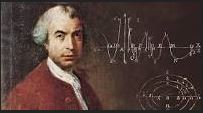
\includegraphics[height=.33\textheight,width=.33\textwidth]{boscovich.jpg}
\end{figure}
\begin{figure}
Karl F. Gauss
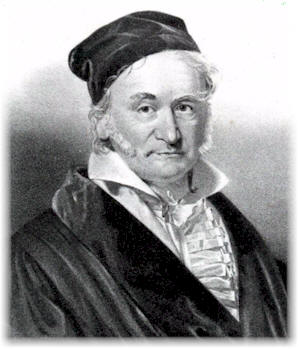
\includegraphics[height=.33\textheight,width=.33\textwidth]{gauss.jpg}
\end{figure}
\onslide<2->{\center --------------------------------------------------------------------}
\end{frame}
\begin{frame}
  \onslide<1->{\frametitle{Least Squares Luminaries} }
\begin{figure}
Peter Swerling
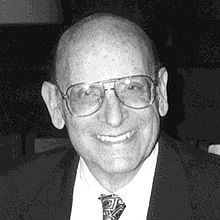
\includegraphics[height=.33\textheight,width=.33\textwidth]{Peter_Swerling.jpg}
\end{figure}
\begin{figure}
Rudolf Kalman
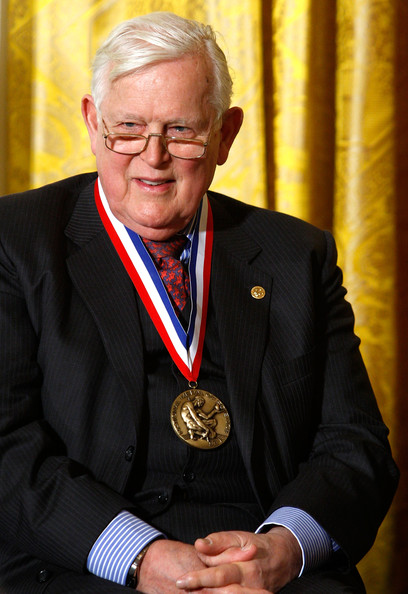
\includegraphics[height=.33\textheight,width=.33\textwidth]{RudolfKalman.jpg}
\end{figure}
\onslide<2->{\center --------------------------------------------------------------------}
\end{frame}

\begin{frame}
\onslide<1->{\frametitle{Kalman Filter Overview}
\framesubtitle{History}}
\begin{itemize}
\onslide<2->{\item Used in early 1960s by Schmidt on Apollo program}
\onslide<3->{\item  Kalman filters are now ubiquitous, especially in navigation}
  \begin{itemize}
     \onslide<4->{
       \item But also in signal processing, econometrics, finance, seismology, weather forecasting, sensor tracking
     }
  \end{itemize}
\end{itemize}
\onslide<5->{\center --------------------------------------------------------------------}
\end{frame}

\begin{frame}
\onslide<1->{\frametitle{Kalman Filter Overview}
\framesubtitle{KF uses in GPS}
}
\begin{itemize}
\onslide<2->{\item All three segments have Kalman filters}
\onslide<3->{\item CS:  ECEST = Ephemeris and Clock Estimator (legacy term), RTGx (JPL's Real-Time GPSY) and NRL's Ensemble Time Filter}
\onslide<4->{\item AEP's ECEST estimates inertial positions and velocities of SVs, solar pressure parameters, 
SV and MS clock error dynamics, and troposphere state at each MS}
\end{itemize}
\onslide<5->{\center --------------------------------------------------------------------}
\end{frame}

\begin{frame}
\onslide<1->{\frametitle{Kalman Filter Overview}
\framesubtitle{KF uses in GPS}
}
\begin{itemize}
\onslide<2->{\item In User Segment receivers, satellite nav software, and offline computations}
\onslide<3->{\item E.g., used in aircraft Operational Flight Programs (OFPs) and Inertial Navigation Systems (INSs) to integrate GPS and other external 
navaids to optimally estimate INS error states }
\onslide<4->{\item 1990s:  Paradigm shift in navigation:\\
  Was: "INS/GPS"\;\;\;\;  Is: "GPS/INS" }
\end{itemize}
\onslide<5->{\center --------------------------------------------------------------------}
\end{frame}


\begin{frame}
\onslide<1->{\frametitle{Kalman Filter Overview}}
\begin{itemize}
\onslide<2->{
	\item State estimation as branch of applied mathematics: 
	Kalman filtering uses techniques and results from many mathematical subjects:\\
linear algebra, differential equations, measure theory, probability, statistics, functional analysis (Hilbert space) 
}
\onslide<3->{
	\item But essentials are very intuitive
}	
	\begin{itemize}
	\onslide<4->{
		\item Can be understood with minimal math background (matrix algebra, calculus, probability and statistics )
	}
	\end{itemize}
\end{itemize}
\onslide<5->{\center --------------------------------------------------------------------}
\end{frame}


\input{\dayonesegone/heuristic_main.tex}
% day1_seg2_equations/equation_main.tex


\begin{frame}

\onslide<1->{\frametitle{Part 1}
 \framesubtitle{Equation Drilldown\\Topics}
 }
\begin{itemize}
 
\onslide<1->{\item Understanding the Notation
 }
\onslide<2->{\item Examples
 }
\onslide<3->{\item Exercises
}
\end{itemize}

\end{frame}




% day1_seg1_heuristic/summary.tex

\begin{frame}
  \onslide<1->{\frametitle{Mathematical Formulation of the Problem} 
  \framesubtitle{Kalman Filter Problem Summary}
  }
 \begin{itemize}
  \onslide<2->{   \item Given two models:}
    \begin{itemize}
  	\onslide<3->{\item State Dynamics Model\\ (sometimes called the System or Process Model)}
  	\onslide<4->{\item Measurement Model\\ (sometimes called the Observation Model)}
    \end{itemize}
  \onslide<5->{ \item Find a way to \textbf{optimally} combine our knowledge of the \textbf{predicted state estimate} 
   with our knowledge of the \textbf{actual measurement} to produce an \textbf{updated state estimate}}
  \begin{itemize}
    \onslide<6->{ \item I.e., find the optimal gain with which to weight the measurement residual (difference between actual and predicted measurement) 
	}
    \onslide<7->{ \item Use weighted residual to  increment or update the state estimate} 
	\onslide<8->{ \item Use Kalman gain also to update the estimation uncertainty  
	(estimation error covariance aka "covariance")}
  \end{itemize}
 \end{itemize}
\onslide<9->{\center --------------------------------------------------------------------}

\end{frame}

\begin{frame}
  \onslide<1->{
  \frametitle{Mathematical Formulation of the Problem}
    \framesubtitle{Kalman Filter Problem Summary\\General, Non-Linear, Time-Invariant,
Discrete-Time Formulation }
}
Given:
 \begin{itemize}
   \onslide<2->{ \item State Dynamics Model:  $x(k)=f[x(k-1)] + w(k)$}
   \begin{itemize}
      \onslide<3->{ \item $k$ indicates the time step;  the actual time at that time step is $t_k$, and the time increment is $\Delta t = t_k - t_{k-1}$}
      \onslide<4->{ \item $x(k)$=state vector,$\;\;f$=true dynamics function,$\;\;w(k)$=process noise}
   \end{itemize}
   \onslide<5->{ \item Measurement Model: $z(k)=h[x(k)]+v(k)$}
   \begin{itemize}
      \onslide<6->{ \item $z(k)$=measurement,$\;\;h$=measurement function, $\;\;v(k)$=measurement noise}
   \end{itemize}
  \end{itemize}
  \onslide<7->{ Find:}
 \begin{itemize}
  \onslide<8->{ \item Optimal gain $K(k)$ that allows us to update our state estimate in the following way:\\
     $\hat{x}(k) = f[\hat{x}(k-1)] + K(k)\;[\;z(k)-h(f[\hat{x}(k-1)])\;]$}
  \onslide<9->{ \item (For now, we'll ignore the update of the covariance)}
\end{itemize}
\onslide<10->{\center --------------------------------------------------------------------}
\end{frame}

\begin{frame}
  \onslide<1->{\frametitle{Mathematical Formulation of the Problem} 
  \framesubtitle{Kalman Filter Problem Summary\\
  Limitations}
  }
 \begin{itemize}
  \onslide<2->{ \item Original Kalman filter solution applies only to ...} 
  \begin{itemize}
\onslide<3-> {\item linear systems with linear measurements driven by ...} 	 
\onslide<4-> {\item zero-mean, Gaussian white noise processes (for both process and measurement noise)}
\end{itemize}
\onslide<5->{\item Assume from now on that ...}
  \begin{itemize}
  \onslide<6-> {
    \item  Our vector-valued function $f$ is a linear, vector-valued function, i.e., a matrix $\Phi$
}
  \onslide<7->{
  \item $h$ is also a linear, vector-valued function, i.e. a matrix $H$
}
  \end{itemize}

  \onslide<8->{ \item Thus, the problem is to find a gain matrix $K(k)$ such that} 
  \onslide<9->{\center $\hat{x}(k) = \Phi\hat{x}(k-1) + K(k)\;[\;z(k)-H\Phi\hat{x}(k-1)\;]$  }

\end{itemize}
\onslide<10->{\center --------------------------------------------------------------------}

\end{frame}

\begin{frame}
  \onslide<1->{\frametitle{Mathematical Formulation of the Problem}
  \framesubtitle{Kalman Filter Problem Summary\\ Linear Discrete Formulation\\
 }
}
Given:
\begin{itemize}
  \onslide<2->{\item State Dynamics Model:
  $x(k)=\Phi x(k-1)+w(k)$}
  \onslide<3->{
    \begin{itemize}
		\item $x(k)$=state vector,$\;\;\Phi $=state transition matrix, $\;\;w(k)$=process noise vector
	\end{itemize} }
  \onslide<4->{\item Measurement Model: $z(k)=H x(k)+v(k)$} 
	\begin{itemize}
		 \onslide<5->{\item $z(k)$=measurement vector,$\;\;H$=meas. matrix, $\;\;v(k)$=meas. noise vector}
	\end{itemize}
  \end{itemize}
  \onslide<6->{Find:}
\begin{itemize}
	  \onslide<7->{\item   State estimate in the form\\
 	$\hat{x}(k) = \Phi \hat{x}(k-1) + K(k)[z(k)-H \Phi \hat{x}(k-1)]$ }
\end{itemize}
\onslide<8->{\center --------------------------------------------------------------------}

\end{frame}

\begin{frame}
  \onslide<1->{\frametitle{Mathematical Formulation of the Problem}
\framesubtitle{Kalman Filter Problem Summary \\
Slight Notational Change}
}
\begin{itemize}
  \onslide<2->{  \item The term $\Phi \hat{x}(k-1)$ is the extrapolated state estimate prior to making the measurement update or correction}
  \onslide<3->{  \item To distinguish prior (extrapolated) estimate from updated estimate, we use the following notation:}
   \onslide<4->{  	\[\hat{x}^{-}(k)=\Phi \hat{x}^{+}(k-1)=\text{\textbf{predicted estimate} prior to update}\]}
 \onslide<5->{  \[\hat{x}^{+}(k)=\text{\textbf{updated state estimate}}\] }
  \onslide<6-> {\item Applying $H$ to $\hat{x}^{-}(k)$ yields the \textbf{predicted measurement}}
\end{itemize}
\onslide<7->{\center --------------------------------------------------------------------}

\end{frame}

\begin{frame}
  \onslide<1->{
    \frametitle{Mathematical Formulation of the Problem}
    \framesubtitle{Kalman Filter Problem Solution}
  }
\begin{itemize}
  \onslide<2->{\item Thus, the solution we seek now looks like this:\\}
  \onslide<3->{
    \begin{equation}\label{filtersolution}
       \hat{x}^{+}(k)=\hat{x}^{-}(k)+ K(k)[z(k)-H\hat{x}^{-}(k)]
    \end{equation}
}
\onslide<4-> {
  where $\hat{x}^{-}(k)=\Phi \hat{x}^{+}(k-1) $
}
\onslide<5-> {
  \item This now looks very much like the running average problem!
}
\end{itemize}
\onslide<6->{\center --------------------------------------------------------------------}

\end{frame}



% day1_seg2_equations/notation.tex
\begin{frame}
  \onslide<1->{\frametitle{Understanding Kalman Filter Notation}
\framesubtitle{Drilldown on State Dynamics}
}
 \begin{itemize}
\onslide<2->{ \item State Dynamics Model: $\simplestatedyneq$ }
\onslide<3->{ \item $x(k)$ is the \textit{\textbf{state vector}} with $n$
 elements, written as a column vector:}
\begin{itemize}
\onslide<4->{ \item $x(k)=\state (k)=\statek$}
\end{itemize}
\onslide<5->{ \item The process noise is also a column vector of size $n$:}
	\begin{itemize}
		\onslide<6->{ \item $\procnoise{k}=\procnoisek$}
	\end{itemize}

	\onslide<7->{ \item Some others prefer to make $k$ a subscript;  we choose not to do so, in order to avoid clashes with vector and matrix elements which do by convention use subscripts}

\end{itemize}
\onslide<7->{\center --------------------------------------------------------------------}
\end{frame}

\begin{frame}
  \onslide<1->{\frametitle{Understanding Kalman Filter Notation}
\framesubtitle{Drilldown on State Dynamics}
}
\begin{itemize}
\onslide<2->{ \item Discrete State Dynamics}
\onslide<3->{ \item KF doesn't work for nonlinear dynamics function $f[x(k-1)]$ }
	\begin{itemize}
		\onslide<4->{ \item But nonlinear models can be linearized (more about that later) }
	\end{itemize}
\onslide<5->{ \item Restriction to matrices:  $\simplestatedyneq$}
\onslide<6->{ \item $\stm{k}$ is called the \textbf{state transition matrix}.  It is 
$n\times n$ in size.}
\begin{itemize}
	\onslide<7->{\item If $\Phi$ is derived from a constant-coefficient difference or differential equation, and the time increments $\Delta t$ are constant, there there is no need for the index $k$;  $\Phi$ will then be constant} 
\end{itemize}
\end{itemize}
\onslide<7->{\center --------------------------------------------------------------------}

\end{frame}

\begin{frame}
  \onslide<1->{\frametitle{Understanding Kalman Filter Notation}
\framesubtitle{Drilldown on State Dynamics}
}

\begin{itemize}
\onslide<2->{ \item State Transition Matrix: $\stmeq{k}$}
\onslide<3->{ \item Extrapolates state vector from time step $k-1$ to time step
 $k$ (pulling from past to present)}
\begin{itemize}
	\onslide<4->{\item If $\Delta t = t_k-t_{k-1}$ is constant for all $k$, then we might write $\Phi(\Delta t)$}
\end{itemize}
\onslide<5->{ \item Tells you how the state would evolve \textbf{in the absence of forcing functions}}
\begin{itemize}
	\onslide<6->{ \item Remember: this is still just a model }
	\onslide<7->{ \item  We don't really know
	what the true state is, because the random forcing function (process noise) generates disturbances!}
\end{itemize}

\end{itemize}
\onslide<8->{\center --------------------------------------------------------------------}

\end{frame}

\begin{frame}
  \onslide<1->{\frametitle{Understanding Kalman Filter Notation}
\framesubtitle{Drilldown on State Dynamics}
}

 \begin{itemize}
\onslide<2->{ \item Other factors and terms often play a role in the full state dynamics model}
 \begin{itemize}
\onslide<3->{ \item A matrix $\sdm{k}$ to distribute the Gaussian white noise
 to the states}
\onslide<4->{ \item An additional, deterministic control variable $u(k)$, and
 associated distribution matrix $\Lambda(k)$}
 \onslide<5->{ \item Then the full state dynamics equation would look like this: 
 \[\statedynctrleq\]}
 \end{itemize}
\onslide<6->{ \item In order to focus primarily on the estimation problem, we will generally omit the control variable}
\onslide<7->{ \item Control is obviously an important part of engineering system solutions, so we will consider it occasionally}
\end{itemize}
\onslide<8->{\center --------------------------------------------------------------------}
\end{frame}

\begin{frame}
  \onslide<1->{\frametitle{The Kalman Filter Solution}
\framesubtitle{ State Estimate Extrapolation}
}

\begin{itemize}
\onslide<2->{\item Given an estimate $\stateest{k-1}{+}$ at time $k-1$, we extrapolate it forward in time 
by the state transition matrix:
\begin{equation}\label{stateextrapeq}
\stateextrapeq 
\end{equation}
}
\onslide<3->{\item Q: Why isn't the white noise sequence $w$ included in this extrapolation?}\\  
\onslide<4->{A:  Because the white noise forcing function is a \textbf{zero-mean} process.  
Thus, \textbf{on average}, the equation is homogeneous and we should therefore use the homogeneous solution, i.e., 
the state transition matrix.}
\end{itemize} 
\onslide<5->{\center --------------------------------------------------------------------}
\end{frame}

\begin{frame}
  \onslide<1->{\frametitle{The Kalman Filter Solution}
\framesubtitle{ Covariance Extrapolation}
}

\begin{itemize}
\onslide<2->{\item Q: How certain are we that our solution is right?}\\
\onslide<3->{A: The answer is given by the \textbf{estimation error covariance matrix}, often for brevity just 
called the covariance matrix $P(k)$\onslide<4->{\footnote{\onslide<5->{There are two other covariance matrices involved in KF, but $P$ is often referred to as THE covariance matrix.}}}
}
\onslide<6->{\item Like the state estimate, the covariance matrix is propagated forward in time before being corrected:}
\onslide<7->
{\begin{equation}\label{altcovextrapeq}
\altcovextrapeq
\end{equation}
where $Q(k)$ is a matrix called the \textbf{process noise covariance matrix} }
\onslide<8->{\item $Q(k)$ measures the amount of dispersion in the white noise forcing function $w(k)$}
\onslide<9->{\item Later we'll learn how to define $P(k)$ (at least initially) in terms of the expected error in the estimation $\esterrdef$}
\end{itemize} 
\onslide<10->{\center --------------------------------------------------------------------}
\end{frame}

\begin{frame}
  \onslide<1->{\frametitle{The Kalman Filter Solution}
\framesubtitle{ Covariance Extrapolation}
}
\begin{itemize}
\onslide<2->{\item What does Eq. \eqref{altcovextrapeq} really mean?
  \[ \altcovextrapeq \]
}
\onslide<3->{\item The term $\stm{k}\covmat{k-1}{+}\stm{k}\trans$ represents the effect that the state dynamics 
has on the estimation error covariance}
\begin{itemize}
\onslide<4->{\item P(k) is a positive definite matrix and $\Phi $ tends to increase its norm }
\end{itemize}
\onslide<5->{\item The other term $Q(k)$ represents the increased uncertainty added at each step due to 
the process noise inherent in the system (like all covariance matrices, it is also positive definite) }
\end{itemize} 
\onslide<6->{\center --------------------------------------------------------------------}
\end{frame}



\begin{frame}
  \onslide<1->{\frametitle{Examples}}
\begin{itemize}
 \onslide<2->{\item The Examples present three different models:}
 \begin{itemize}
 \onslide<3->{\item Resistor Revisited (but using a Kalman filter instead of a running average)}
 \onslide<4->{\item Constant Velocity Motion (non-accelerated motion)}
 \onslide<5->{\item Damped Harmonic Oscillator}
\end{itemize}
 \onslide<6->{\item Types of Plots produced by the simulations} 
\end{itemize} 
\onslide<7->{\center --------------------------------------------------------------------}
\end{frame}

\begin{frame}
  \onslide<1->{\frametitle{Overview of the Examples}}
\begin{itemize}
  \onslide<2->{\item Discrete-time systems}
  \onslide<3->{\item Gradually increasing complexity:  }
  \begin{itemize}
    \onslide<4->{\item Resistor: 1 state, \textbf{static} (constant dynamics)  }
    \onslide<5->{\item Constant Velocity Motion:  2 states, with one state \textbf{dynamic} and one \textbf{static} }
    \onslide<6->{\item Damped Harmonic Oscillator:  2 states, with \textbf{both states dynamic}  }
  \end{itemize}
\end{itemize}
\onslide<7->{\center --------------------------------------------------------------------}
\end{frame}

\begin{frame}
  \onslide<1->{
  \frametitle{ The MATLAB/Python files:\\ 
		\texttt{kf\_resistor\_demo,constant\_velocity, damposc} in both .m and .py versions}
}
\begin{itemize}
  \onslide<2->{\item File located here: matlab/python \\
    \url{https://github.com/musicarroll/kalman_course/src }
	}
  \onslide<3->{\item Download these scripts and play with them!  }
  \begin{itemize}
	\onslide<4->{\item Modify the initial conditions, number of samples  }
  	\onslide<5->{\item Modify the $R$ and $Q$ noise parameters  }
	\onslide<6->{\item Observe how the plots change }
  \end{itemize}
  \onslide<7->{ \item If you want to share your mods to the programs, upload them to the 
  student\_contrib folder on github}
  \onslide<8-> {\item Please add a suffix (such as your YouTube ID) to filename:  \\
  E.g. damposc\_joeuser.py
  }
\end{itemize}
\onslide<9->{\center --------------------------------------------------------------------}
\end{frame}


\begin{frame}
  \onslide<1->{\frametitle{Types of Plots}}
\begin{itemize}
  \onslide<2->{\item Truth/Measurement/Estimation (TME) plots}
  \begin{itemize}
	\onslide<3->{\item Time series plots of ground truth model, measurements, and state estimations}
  \end{itemize}
  \onslide<4->{\item Kalman Sawtooth plots}
  \begin{itemize}
    \onslide<5->{\item Specialized plots for simultaneously assessing the growth and reduction in estimation uncertainty }
  \end{itemize}
\end{itemize}
\onslide<6->{\center --------------------------------------------------------------------}
\end{frame}

\begin{frame}
  \onslide<1->{
	\frametitle{TME Plots} 
	\framesubtitle{Truth, Measurement, Estimation Plots}
}
  \onslide<2->{
\begin{figure}
  \includegraphics[width=0.95\textwidth,height=7cm]{\dayonesegtwo/damposc_conservative.png}
\end{figure}   
}
\onslide<3->{\center --------------------------------------------------------------------}
\end{frame}


\begin{frame}
  \onslide<1->{\frametitle{Kalman Sawtooth Plots}}
  \begin{itemize}
   \onslide<2->{\item Interleave pre- and post-update elements of $P$ over a run
   }
   \onslide<3->{\item Show growth over time in uncertainty (upticks) and 
   then immediate reduction (no time lapse!) in uncertainty (downticks) after measurement updates 
}
\onslide<4->{   
\begin{figure}
  \includegraphics[width=0.75\textwidth,height=5cm]{\dayonesegtwo/kf_resistor_variance_w_process_noise.png}
\end{figure}
}
\end{itemize}
\onslide<5->{\center --------------------------------------------------------------------}
\end{frame}


%\input{\dayonesegtwo/03_01_resistor.tex}
%\input{\dayonesegtwo/03_02_constant_velocity.tex}
%\input{\dayonesegtwo/03_03_damposc.tex}





% day1_seg2_equations/exercises.tex

\begin{frame}

  \onslide<1->{\frametitle{Exercises
}}
\begin{enumerate}
  \onslide<2->{\item Work through the resistor example by hand using 
$\hat{x}_0=100\Omega$, $\sigma=0.1$, and $P_0=0$.  Start the recursive loop 
with the gain equation first.  Run through the loop three times.}

  \onslide<3->{
\item Draw a rough plot of the error covariance, plotting both the extrapolated and 
updated covariance for any give $k$ at the same time.  (This will yield the classic 
Kalman sawtooth pattern.)
  Similarly, draw a rough plot of the state estimates.}

\setcounter{exercisecounter}{\value{enumi}}
\end{enumerate}
\end{frame}


\begin{frame}


  \onslide<1->{\frametitle{Exercises
}}
\begin{enumerate}
\setcounter{enumi}{\value{exercisecounter}}
  \onslide<2->{\item Calculate the Kalman gain of the non-accelerated motion example.  Hint:  It looks a lot like the 
gain for the damped harmonic oscillator.}
  \onslide<3->{\item Write out the state update equation for the damped harmonic oscillator, 
using the Kalman gain derived in the example.

}
  \onslide<4->{\item Write out the covariance update 
equation for the damped harmonic oscillator, using the Kalman gain dervied in the 
example.
 }
\end{enumerate}
\end{frame}


% % day1_seg2_diff_eq/state_space_main.tex
\begin{frame}
\textbf{Segment 3\\
Differential Equations and Difference Equations\\
Topics}
 \begin{itemize}
   \item Input-Output Representation
   \item Differential Equations and Difference Equations
\end{itemize}
\end{frame}
% day1_seg3_state_space/input_output.tex

\begin{frame}
Input-Output Representation
 
\begin{itemize}
 
\item Black box approach:  $y(t)=f(u(t),t)$\\

 
\begin{figure}
   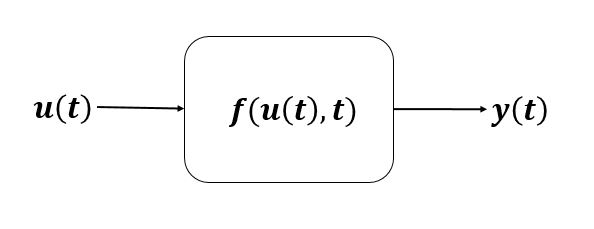
\includegraphics[width=0.85\textwidth]{day1_seg3_diff_eq/input_output.jpg}

 
\end{figure}
\item Output represents the resultant behavior of the dynamic system as a function 
of the input (and possibly time).
 
\item Output is often one primary scalar variable of interest like position.

\end{itemize}

\end{frame}



\begin{frame}
Input-Output Representation
 
\begin{itemize}
 
\item Note that output is not necessarily the same thing as the observation or measurement.
 
\item Observation or measurement is often related directly to the output through a matrix coupling.
 
\item In state space representation, the output is often eliminated in favor of the state vector, and 
the measurement is given as a function of the state vector directly.

\end{itemize}

\end{frame}



\begin{frame}
Input-Output Representation
 
\begin{itemize}
 
\item The derivatives of position and how they relate to the forcing function yields a single differential equation.
 
\item We'll see later how an $n^\text{th}$-order, scalar differential equation is related to a 
vector state space model. 



\begin{itemize}
  \item In fact, the state vector be comprised of the values of the initial conditions for the differential 
equation at any particular time.
\end{itemize}


\end{itemize}

\end{frame}

% day1_seg3_diff_eq/diff_eq.tex

\begin{frame}
Differential Equations and Difference Equations
\\
A Mini Refresher Course 
\begin{itemize}
 
\item Ordinary Differential Operators
 
\item Ordinary Differential Equations
 
\item Difference Equations

\end{itemize}

\end{frame}


% orddiffops.tex

\begin{frame}
Ordinary Differential Operators: Vectors and Functions

\begin{itemize}
  \item Vectors are functions and functions are vectors
  
\item A vector $\begin{bmatrix}x_1\\x_2\\x_3\end{bmatrix}$ in 3-space is really a 
function $x:\set{1,2,3}\rightarrow \Real$
  
\item We just write them differently than functions, i.e., instead of $x(i)$ 
we write $x_i$. 

\end{itemize} 

\end{frame}


\begin{frame}
Ordinary Differential Operators: Vectors and Functions
 
\begin{itemize}
  
\item And since the domain $\set{1,2,3}$ of the function $x$ is so small, we can 
exhibit all values of $x$ explicitly in one fell swoop, i.e., 
as $\begin{bmatrix}x_1\\x_2\\x_3\end{bmatrix}$
  
\item But, by the same token, ordinary real functions $f:\Real\rightarrow\Real$ are 
vectors
  
\item They just have so many components that we can't exhibit them all at once

\end{itemize} 

\end{frame}


\begin{frame}
Ordinary Differential Operators: Vectors and Functions

\begin{itemize}
  
\item We can add vectors by adding their components: $z=x+y$ if and only if 
$z_i=x_i+y_i$ for each index $i$
  
\item By the same token, we can add functions componentwise:
  $h=f+g$ if and only 
if $h(t)=f(t)+g(t)$ for all $t$ in the domain
  
\item Componentwise multiplication of functions can also be defined 
(although this does not come up as often for ordinary vectors):  $h=f\cdot g$ if 
and only if $h(t)=f(t)\cdot g(t)$ for all $t$ in the domain

\end{itemize} 

\end{frame}



\begin{frame}
Ordinary Differential Operators: Vectors and Functions

\begin{itemize}
  
\item Finally, we can multiply functions by scalars, just like we do for vectors:  
$g=a\cdot f$ if and only if $g(t)=a\cdot f(t)$ for all $t\in\Real$.
  
\item The upshot of all this is that the set of all real functions is a vector space!
  
\item But we are really more interested in a subspace of this vector space, i.e., we really want to 
restrict our attention to the set of all \textbf{differentiable} functions on some closed interval.

\end{itemize} 

\end{frame}


\begin{frame}
Ordinary Differential Operators: Differentiable Functions

\begin{itemize}
  
\item Let $I=[a,b]$ be any closed interval of the real line
  
\item Consider the set $\Real^I=\set{f:I\rightarrow \Real}$ of all functions mapping $I=[a,b]$ into the real numbers
  
\item Then, as we have just pointed out, $\Real^I$ is a vector space over the reals

\end{itemize} 

\end{frame}



\begin{frame}
Ordinary Differential Operators
 
\begin{itemize}
  
\item We define the \textbf{\textit{derivative}} of a function $f$ at the point $t\in [a,b]$ as the 
limit as $s\rightarrow
 t$ of the difference quotient,
 \[\frac{f(s)-f(t)}{s-t},\]
assuming this limit exists.
  
\item Note that not all functions have derivatives!
  
\item Those that do have a derivative defined at every point of $I$ we call \textbf{\textit{differentiable}} on $I$.

\end{itemize} 

\end{frame}



\begin{frame}
Ordinary Differential Operators
 
\begin{itemize}
  
\item This operation turns out to be a linear operator on the vector space of functions that are differentiable 
on $I=[a,b]$.
  
\item In fact, we want to consider those functions that can be differentiated as many times as we like
  
\item Thus, we consider the space of infinitely differentiable, real-valued functions defined on the 
closed real interval $[a,b]$: $C^\infty[a,b]$
\end{itemize}

\end{frame}


% orddiffeqs.tex

\begin{frame}
Ordinary Differential Operators
 
\begin{itemize}
 
\item The operation of taking the derivative will enable us to develop deterministic differential
 equations.
 
\item Later we will define derivatives of stochastic processes in order to introduce and solve stochastic 
differential equations.  You cannot always take the derivative (or even integrate) a random process -- 
and sometimes not even the sample functions of a random process -- in the ordinary sense.

\end{itemize}

\end{frame}


% orddiffeqs.tex

\begin{frame}
Ordinary Differential Operators
 
\begin{itemize}
 
\item Since the derivatives of all orders are assumed to exist
 for all functions $f\in C^\infty[a,b]$, the 
limit of the
 difference quotient always exists for such functions.
 
\item Thus, we assign to each $f$ a new function $Df$ given by

\begin{equation}\label{deriv}
  [Df](t) = \lim_{s\rightarrow t}\frac{f(s)-f(t)}{s-t}
\end{equation}
 
\item This assignment defines a transformation
 \[D:C^\infty[a,b]\rightarrow C^\infty[a,b]\]
  that is a linear operator.

\end{itemize}

\end{frame}


\begin{frame}
Ordinary Differential Operators
 
\begin{itemize}
    
\item $D$ is linear: $D[af+bg]=a[Df] + b[Dg]$
    
\item Sometimes we get lax and simply write $Df(t)$ instead of $[Df](t)$.  However, keep in mind that $Df(t)$ 
says "Differentiate $f$ and then evaluate the resulting function at the point $t$."
    
\item $D$ obeys all the usual rules of differential calculus such as the product rule and the chain rule:

\[D(fg)=[Df]g+f[Dg]\]
\[D(f\circ g) = [Df]\circ g \cdot Dg\]
 
\end{itemize}

\end{frame}


\begin{frame}
Ordinary Differential Operators: Examples
 
\begin{itemize}
  
\item If $\id$ is the identity function, i.e., $\id(t)=t$, then
 $D\id=1$. (You probably know this 
as $\frac{dt}{dt}=1$; Note that 1 is the function whose value at every $t$ is 1.)
  
\item Using the product rule, we have, for example,

\begin{align*}
D\id^2 &= D\left[\id \cdot \id \right]\\
&= D\id \cdot \id + \id \cdot D\id\\
&= 1 \cdot \id + \id \cdot 1\\
&= \id + \id\\
&= 2\id
\end{align*}

(In more familiar notation this is just $\frac{dt^2}{dt}=2t$.)
 
\end{itemize}

\end{frame}


% orddiffeqs.tex

\begin{frame}
Ordinary Differential Operators
 
\begin{itemize}

 \item Note that we sometimes write $d/dt$ or $\frac{d}{dt}$ for
 the operator $D$ when we want to emphasize 
the independent
 variable $t$.  Or, instead of $\frac{dy}{dt}$ we write simply $\dot{y}$.
 
\item However, that is really unnecessary, adds no new information, and is just extra
 baggage.
 
\item Nevertheless, we shall do it sometimes because it may be more familiar.

\end{itemize}

\end{frame}


% orddiffeqs.tex

\begin{frame}
Ordinary Differential Operators
 
\begin{itemize}
 
\item Since there is really only one generating operator $D$ that we are interested in here,
 
we are less interested in multiplication than we are in function
 composition or iteration of this operator. 
For instance,
 $D^2f=[D\circ D](f) = D(Df)$.
 
\item By induction we have $D^n=\underbrace{D\circ\cdots \circ D}_n$.
 
\item Just as real-valued functions inherit algebraic operations from those of their range
 spaces, 
so too do differential operators:
 \[\left[aD^m+bD^n\right](f)=a(D^mf)+b(D^nf)\]

\end{itemize}

\end{frame}


% orddiffeqs.tex

\begin{frame}
Ordinary Differential Operators
 
\begin{itemize}
 
\item We can therefore generate polynomials in $D$:
 \[p(D)=a_nD^n+\cdots +a_1D+a_oI,\]
 
where $I$ is the identity operator on $C^\infty[a,b]$.  We
 usually just drop the identity operator, 
since it amounts to multiplying by 1.
 
\item Such polynomials in $D$ are still linear operators.
 
\item Thus, we have rediscovered the group
 ring $\Real(\Diff)$, where $\Diff$ in this case is the 
infinite cyclic
 group generated by the differential operator $D$.  We'll call
 this group ring 
 
the \textit{\textbf{polynomial ring of differential operators}}.

\end{itemize}

\end{frame}


\begin{frame}
Ordinary Differential Equations
 \begin{itemize}
 \item With polynomials of differential operators we can now
 define ordinary differential equations.
 \item An equation of the form
 \[p(D)f=q(D)g\]
 where  $f,g\in \Cinf$ and $p(D),q(D)\in \Real(\Diff)$,
 is called an ordinary differential equation with constant
 coefficients.
\end{itemize}
\end{frame}
% orddiffeqs.tex
\begin{frame}
Ordinary Differential Equations
 \begin{itemize}
 \item It is probably more familiar if we use $y$
 instead of $f$ and $u$ instead of $g$, and if we show the
 independent variable, say t, explicitly:
 \[a_n\frac{d^ny}{dt^n}+\cdots +a_1\frac{dy}{dt}+a_0y =
 b_m\frac{d^mu}{dt^m}+\cdots + b_1\frac{du}{dt}+b_0u\]
 or
\begin{equation}\label{diffeq}
\diffeq
\end{equation}
 \item For our purposes, the function $u=u(t)$ is called the \textit{\textbf{input}},
 while the function $y=y(t)$ is called the \textit{\textbf{output}}.  The
 independent variable $t$ is thought of as time.
\end{itemize}
\end{frame}
\begin{frame}
Ordinary Differential Equations
 \begin{itemize}
 \item In \eqref{diffeq}, $u$ is ordinarily assumed to be known or given,
 while $y$ is unknown and sought.
 \item Any function $y$
 satisfying \eqref{diffeq} is called a solution of the
 differential equation.
 \item A differential equation such as \eqref{diffeq} is called
 \textit{\textbf{homogeneous}} when the input function $u$ is identically zero
 for all $t\in[a,b]$.
\end{itemize}
\end{frame}
\begin{frame}
Ordinary Differential Equations
 \begin{itemize}
 \item Thus far we have only dealt with linear differential equations
 with constant coefficients.
 \item We could allow the coefficients to be time-dependent
 functions.  However, for most of our applications, this will not
 be necessary.
\end{itemize}
\end{frame}
% orddiffeqs.tex
\begin{frame}
Ordinary Differential Equations: Examples
 \begin{itemize}
 \item From physics we have Hooke's law: the restoring force of a
 spring is proportional to the distance stretched:  $-ky = m\frac{d^2y}{dt^2}$.
 \item This is just an application of Newton's $F=ma$, where $a$
 is the acceleration: $a=d^2y/dt^2$.
 \item Rewriting this in the form of \eqref{diffeq} we have
 \[m\frac{d^2y}{dt^2}+ky=0\]
 \item Therefore, this is a homogeneous equation of order 2.
\end{itemize}
\end{frame}
% orddiffeqs.tex
\begin{frame}
Ordinary Differential Equations
 \begin{itemize}
 \item We have used $y$ rather than $x$ as in most physics books,
 because we want to be consistent with \eqref{diffeq}.
 \item It is common to rewrite such equations so that the leading
 coefficient is 1.  Thus we have:
 \[\frac{d^2y}{dt^2}+\frac{k}{m}y=0.\]
 \item It is easily verified that $\sin\omega_0 t$, where
 $\omega_0=\sqrt{\frac{k}{m}}$, satisfies this differential equation.
\end{itemize}
\end{frame}
\begin{frame}
Ordinary Differential Equations
 \begin{itemize}
 \item Equation \eqref{diffeq}
 \[\diffeq\]
 is called
 \textit{\textbf{time-invariant}}, because the coefficients are
 constant and also because the independent variable $t$ does not
 appear explicitly in the equation.
 \item Note that \eqref{diffeq} is linear in terms of both the
 input and the output, because the polynomial differential
 operator on each side of the equation is a linear operator.
\end{itemize}
\end{frame}
\begin{frame}
Ordinary Differential Equations
 \begin{itemize}
 \item This double linearity means, on the one hand, that the output $y$ due to several inputs acting
 at the same time is equal to the sum of the outputs due to each
 input acting alone.
 \item On the other hand, it also means that if $y_1$ and $y_2$
 are both solutions to the homogeneous version of \eqref{diffeq},
 then so is $c_1y_1+c_2y_2$ where $c_1$ and $c_2$ are any real
 constants.
 \item A maximal set of $n$ such solutions to the homogeneous
 equation that are also linearly independent (as vectors) is
 called a \textit{\textbf{fundamental set}}.
\end{itemize}
\end{frame}
\begin{frame}
Ordinary Differential Equations
 \begin{itemize}
 \item You can find a fundamental set by solving the
 \textit{\textbf{characteristic equation}} associated with the differential equation.  This equation is
 nothing other than the original polynomial equation in $D$, but
 with $D$ replaced by an unknown such as $z$.
 \item Thus, the characteristic equation for \eqref{diffeq} is
 \[a_nz^n+\cdots + a_1z + a_0=0\]
 \item We use $z$ because the roots of this equation are in
 general complex (thanks, once again, to Dr. Gauss).
\end{itemize}
\end{frame}
\begin{frame}
Ordinary Differential Equations
 \begin{itemize}
 \item In solving the characteristic equation, two cases emerge:
 \begin{enumerate}
 \item The roots of the characteristic equation are all distinct.
 \item Some roots are repeated, i.e., each root $r_i$ has
 multiplicity $n_i$.
 \end{enumerate}
\end{itemize}
\end{frame}
\begin{frame}
Ordinary Differential Equations
 \begin{itemize}
 \item In case 1, a fundamental set is easily constructed:
 \[y_1(t)=\exp(r_1t),\ldots,y_n(t)=\exp(r_nt) \]
 where the $r_i$ are the distinct roots.
 \item In case 2, each root $r_i$ of multiplicity $n_i$ contributes
 $n_i$ functions to the fundamental set:
 \[y_{i1}(t)=\exp(r_it),y_{i2}(t)=t\exp(r_it),\ldots,y_{in_i}(t)=t^{n_i-1}\exp(r_it) \]
\end{itemize}
\end{frame}
\begin{frame}
Ordinary Differential Equations
 \begin{itemize}
 \item To fully solve the differential equation, the initial
 conditions need to be taken into account.
 \item These are the values of the function and its first $n-1$
 derivatives at the start of the time interval.
 \item We will specialize our interval $[a,b]$ to the case in which $a=0$
 and $b=T$, some unspecified time in the future.
\end{itemize}
\end{frame}
\begin{frame}
Ordinary Differential Equations
 \begin{itemize}
 \item The \textit{\textbf{free response}} is the solution to the homogeneous
 equation in which the initial conditions are specified but the input is zero, i.e., there is no forcing function.:
\begin{equation}\label{initcond}
  y(0),Dy(0),\ldots,D^{n-1}y(0)
\end{equation}
 \item The \textit{\textbf{forced response}} reverses this situation; it allows the
 input function to be non-zero, but it requires all the initial
 conditions in \eqref{initcond} to be zero.
 \item The \textit{\textbf{total response}} is the sum of the free and forced
 responses.
\end{itemize}
\end{frame}
\begin{frame}
Ordinary Differential Equations: Example of Free, Forced and Total
Responses
 \begin{itemize}
 \item Consider $D^2y+3Dy-1y=u$ with initial conditions:
 $y(0)=1,Dy(0)=-1$.
 \item The roots (found using Matlab's roots function) are $r_1=-3.3028$ and $r_2=0.3028$, and they are
 distinct.
 \item Therefore, a fundamental set is
 $\set{\exp(-3.3028t),\exp(0.3028t)}$.
\end{itemize}
\end{frame}
\begin{frame}
Ordinary Differential Equations: Example of Free, Forced and Total
Responses
 \begin{itemize}
 \item With the fundamental set and the initial conditions we can
 form a set of $n$ linear equations in $n$ unknowns (here, $n=2$):
\begin{align*}
  c_1y_1(0)+c_2y_2(0) & =y(0) \\
  c_1Dy_1(0)+c_2Dy_2(0) & =Dy(0)
\end{align*}
or
\begin{align*}
  1\cdot c_1+1\cdot c_2 & =0 \\
  -3.3028\cdot c_1+0.3028\cdot c_2 & =-1
\end{align*}
\end{itemize}
\end{frame}
\begin{frame}
Ordinary Differential Equations
 \begin{itemize}
 \item The previous linear system is of the form $Ax=b$.  Using
 Matlab's matrix division operator $\backslash$, the solution is
 $x = A\backslash b$ or
\begin{align*}
  c_1 & =    0.2773 \\
  c_2 & =   -0.2773
\end{align*}
%\item We can easily verify that
%$y(t)=0.2773\exp(-3.3028t)-0.2773\exp(0.3028t)$ is indeed the free
%response by plugging and chugging
%\begin{align*}
%  D^2y+3Dy-1y & =D^2[0.2773\exp(-3.3028t)-0.2773\exp(0.3028t)]\\
%   & \quad +3D[0.2773\exp(-3.3028t)-0.2773\exp(0.3028t)]\\
%   & \quad -1[0.2773\exp(-3.3028t)-0.2773\exp(0.3028t)] \\
%   & = 0.2773\cdot 3.3028^2\exp(-3.3028t)\\
%   & \quad -0.2773\cdot 0.3028^2\exp(0.3028t)\\
%   & \quad +3\cdot 0.2773\cdot (-3.3028)\exp(-3.3028t)\\
%   & \quad -3\cdot 0.2773\cdot 0.3028\exp(0.3028t)\\
%   & \quad -0.2773\exp(-3.3028t)+0.2773\exp(0.3028t)
%\end{align*}
\end{itemize}
\end{frame}
\begin{frame}
Ordinary Differential Equations
 \begin{itemize}
 \item The total response can also be decomposed into transient
 and steady state responses
 \item The \textit{\textbf{transient}} response is that part of the total response
 that decays to 0 as $t\rightarrow \infty$.
 \item The \textit{\textbf{steady state response}} is the difference between the
 total response and the transient response.
\end{itemize}
\end{frame}
\input{day1_seg3_diff_eq/lti.tex}


% difference_eq.tex
\begin{frame}
Ordinary Difference Equations
\begin{itemize}
  \item Auto-Regressive Moving Average (ARMA)
  \item $n^{\text{th}}$ derivative corresponds to $n$-step advance:
\end{itemize} 
\begin{equation}\label{armaeq}
\armaeq
\end{equation}
\end{frame}
\begin{frame}
Ordinary Difference Equations
\begin{itemize}
  \item The left side of Eq. \eqref{armaeq} is the Auto-Regressive part
  \item The right side of Eq. \eqref{armaeq} is the Moving Average part
  \item Hence, ARMA
\end{itemize} 
\end{frame}
\begin{frame}
Ordinary Difference Equations: Example
\begin{itemize}
  \item Let $n=3$, $m=2$ and consider the difference equation:
\begin{align*}
-3y(k+3)+1.5y(k+2)\\
 +7y(k+1)-3.2y(k)\\
&=23u(k+2)-5u(k+1)+0.5u(k)
\end{align*}
\end{itemize} 
\end{frame}



% \input{day1_seg3_state_space/stoch_diff_eq.tex}
%% day1_seg3_state_space/exercises.tex
\begin{frame}
Exercises
 \begin{itemize}
 \item
 \item
 \item
\end{itemize}
\end{frame}


\begin{frame}
  \onslide<1->{\frametitle{State Space Concepts}
\framesubtitle{Topics} 
}
\begin{itemize}
  \onslide<2->{
\item  Dynamic Systems: Differential Equations and the Concept of State Space
}
  \onslide<3->{
\item  Diagrams and State Space 
}
  \onslide<4->{
\item   State Transition Matrix
}
\end{itemize}
\onslide<5->{\center --------------------------------------------------------------------}
\end{frame}

% \input{day1_seg3_state_space/stoch_diff_eq.tex}


\begin{frame}
  \onslide<1->{\frametitle{Dynamic Systems} 
  \framesubtitle{The Concept of State Space}
}
  
\begin{itemize}
  \onslide<2->{
\item Time-dependent behavior of physical systems often
 modeled analytically by \emph{differential equations}
}
  \onslide<3->{
\item  Called \textit{\textbf{dynamic systems}} or
 \textit{\textbf{dynamical systems}}
}
  \onslide<4->{
	\item  Smooth processes:  described by continuous, differentiable functions of time
}
\end{itemize}
\onslide<5->{\center --------------------------------------------------------------------}
\end{frame}


\begin{frame}
	\onslide<1->{\frametitle{Dynamic Systems}
	\framesubtitle{Newton's Laws of Motion} }
	\begin{itemize}
		\onslide<2->{
			\item Newton's first two laws specify what happens when a body is subjected to a force.   
		}
		\onslide<3->{
			\item Whenever a net force acts on a body, the body's velocity will change, i.e., it will accelerate or decelerate  (First Law)
		}
		\onslide<4->{
			\item For a constant net force, the motion will be such that the product of the body's mass and its acceleration will be invariant (i.e., the same for all bodies) (Second Law)
		}
		\begin{itemize}
		\onslide<5->{
			\item Under the same constant force, large bodies will exhibit a small acceleration, while small bodies will exhibit a larger acceleration
		}
		\end{itemize}
	\end{itemize}
	\onslide<6->{\center --------------------------------------------------------------------}
\end{frame}



\begin{frame}
  \onslide<1->{\frametitle{Dynamic Systems}
  \framesubtitle{Newton's Laws of Motion}
 }
\begin{itemize}
  \onslide<2->{
\item In Newton's Second law $F=ma$, the resultant force $F$ acts on the mass $m$ to produce an acceleration:
\begin{equation}
F=ma=m\dot{v}=m\deriv{v}{t}=m\secondderiv{y}{t}=m\ddot{y}
\end{equation}  
}
  \onslide<3->{
	\item Since acceleration is the second derivative of position, Newton's Second law often leads to \textbf{second order} differential equations (whenever the acceleration is constant, i.e., $\dot{a}=0$); the solution $y(t)$ is considered to be the \textbf{output} of the dynamical system   
}
  \onslide<4->{
	\item The resultant force is the vector sum of all forces acting on the body, both \textbf{internal} coupling forces and \textbf{external} input forces  
}
\end{itemize}
\onslide<5->{\center --------------------------------------------------------------------}
\end{frame}

\begin{frame}
	\onslide<1->{\frametitle{Dynamic Systems} 
	\framesubtitle{A Note on Notation}
	}
	\begin{itemize}
		\onslide<2->{ \item In pure mathematics, one often sees $y$ as a function of $x$:  $y=f(x)$.  
		}
		\onslide<3->{
			\item  However, in engineering work, the variable $x$ is often reserved to be used as the (vector) state variable.
		}
		\onslide<4->{
			\item Moreover, in dynamic systems, $y$ is generally considered to be a function of time $t$.  Hence our use of symbols such as \\ $y(t)$, $\dfrac{dy}{dt}$, $\Dopnth{n}{t}{y}$, $\dot{y}$, $\ddot{y}$, etc.
		}
		\onslide<5->{
			\item  In physics, the variable $r=r(t)$ is often used to stand for displacement (position), with 3d coordinates of $x,y,z$.
		}
		\onslide<6->{
			\item In these slides we are mostly using standard engineering notation.
		}
		\onslide<7->{
			\item It is also common in engineering notation to use $u=u(t)$ as the symbol for external input -- or control -- function.
		}
	\end{itemize}
	\onslide<8->{\center --------------------------------------------------------------------}
\end{frame}

\begin{frame}
  \onslide<1->{\frametitle{Dynamic Systems}
	\framesubtitle{Internal and External Forces}  
}
\begin{itemize}
  \onslide<2->{ \item Which forces are considered internal and which external depends on how the system boundary is drawn  
}
  \onslide<3->{
\item  Simple harmonic oscillator has one internal force determining system behavior: $F=-ky$, because the spring itself is often considered a (massless) part of the system  \\(more complicated oscillators may also include internal frictional and/or external driving forces)
}
\onslide<4->{
	\item Spring forces (e.g., Hooke's law, where $F=-ky$) are often considered to be \textbf{internal} to system
}
  \onslide<5->{
\item  External forces (e.g., constant or time-dependent forcing functions) may also be present, e.g.:
 \[\frac{d^2y}{dt^2}+\frac{k}{m}y=\dfrac{1}{m}\sin\omega t\]
}
\onslide<6->{
	\item Internal forces are generally not viewed as \textbf{inputs}
}
\end{itemize}
\onslide<7->{\center --------------------------------------------------------------------}
\end{frame}

\begin{frame}
  \onslide<1->{\frametitle{Dynamic Systems} 
	\framesubtitle{Second-Order Mechanical Systems}
}
\begin{itemize}
  \onslide<2->{
\item Most general second-order equation for a mechanical
 system of this type (according to Newton's law) is:
\begin{equation}\label{second ord}
 \ddot{y} =\frac{1}{m}F(y,\dot{y},t)
\end{equation}  
}
  \onslide<3->{
\item If $F(y,\dot{y},t)$ can be expressed 
as sum of $F_1(y,\dot{y})$ and $F_2(t)$, then
 we can write this in input-output form:
  \[\ddot{y}-\frac{1}{m}F_1(y,\dot{y})=\frac{1}{m}F_2(t)\]
}
  \onslide<4->{
	\item Note that the left hand side is a function only of $y$ and its derivatives, while the right hand side is a function of time only.
}
\end{itemize}
\onslide<5->{\center --------------------------------------------------------------------}
\end{frame}



\begin{frame}
	\onslide<1->{\frametitle{The Concept of State} }
	\begin{itemize}
		\onslide<2->{
			\item Concept of state involves in some sense the instantaneous internal arrangement and relationships of a system's components
		}
		\onslide<3->{
			\item In practical  situations, the state variables may represent attributes of the  system that we wish to know something about 
		}
		\onslide<4->{
			\item Also intuitively, state variables are usually naturally coupled in some sense; 
			this is obvious when they are derived from a single differential equation in which all quantities are derivatives 
			of a single variable (the output variable)  
		}
	\end{itemize}
	\onslide<5->{\center --------------------------------------------------------------------}
\end{frame}


\begin{frame}
  \onslide<1->{\frametitle{The Concept of State} 
	\framesubtitle{State as Initial Conditions}  
}
\begin{itemize}
  \onslide<2->{
	\item \footnotesize{"How is a dynamic system (linear or nonlinear) described?
		The fundamental concept is the notion of the state.  By this is meant, intuitively, some quantitative information 
		(a set of numbers, a function, etc.) which is the least amount of data one has to know about the past behavior of 
		the system in order to predict its future behavior."\\
		Rudolf Kalman, in seminal paper (1960)}
}
  \onslide<3->{
\item To determine behavior of deterministic system at any future time requires knowledge of two things:
\begin{enumerate}
\item Equations governing the system dynamics (usually differential of difference equations)
\item Initial conditions
\end{enumerate}  
}
  \onslide<4->{
\item But initial conditions for an $n^{\text{th}}$-order continuous dynamic system are simply values of first $n$ derivatives at initial time (the Identity operator can be considered the 0th order derivative)
}
  \onslide<5->{
	\item The $n^{\text{th}}$-order derivative is given essentially by the differential equation itself
}

\end{itemize}
\onslide<5->{\center --------------------------------------------------------------------}
\end{frame}

\begin{frame}
  \onslide<1->{\frametitle{The Concept of State} }
\begin{itemize}
  \onslide<2->{
\item At any point in time, we can think of instantaneous values of first $n$ derivatives as initial conditions for all future dynamic evolution  
}
  \onslide<3->{
\item The first $n$ derivatives are the $0^\text{th},1^\text{st},\ldots,(n-1)^\text{st}$ derivatives of the output function $y$
}
  \onslide<4->{
	\item These values capture the "state" of the dynamic system at any time after the time of the initial conditions  
}
\end{itemize}
\onslide<4->{\center --------------------------------------------------------------------}
\end{frame}

\begin{frame}
  \onslide<1->{\frametitle{The Concept of State} 
	\framesubtitle{Relation to Taylor's Series}  
}
\begin{itemize}
  \onslide<2->{
\item  Concept of "state" also encoded in Taylor series of a function 
}
  \onslide<3->{
\item Taylor's theorem: if a function $y(t)$ has derivatives of all orders near $t_0$, then its value at any point $t$ near $t_0$ can be determined from the values of its derivatives at $t_0$:
}
  \onslide<4->{
\begin{equation}
\taylor{y}{t}{t_0}
\end{equation}
}
  \onslide<5->{
	\item I.e., the value of the function at a time near $t_0$ is completely determined by its value and the values of all of its derivatives at $t_0$\\ (Note that this works for time points in the past as well as those in the future, provided they are sufficiently close to $t_0$)
}
\end{itemize}
\onslide<6->{\center --------------------------------------------------------------------}
\end{frame}

\begin{frame}
  \onslide<1->{\frametitle{The Concept of State} 
	\framesubtitle{Relation to Taylor's Series}  
}
\begin{itemize}
  \onslide<2->{
\item In the language of dynamic systems, the quantity $t-t_0$\\ (if $>0$) is simply the time elapsed since the initial time $t_0$ (otherwise, it is the negative duration from $t_0$ to a past time point $t$).  
}
  \onslide<3->{
\item Thus, if you have knowledge of the state at time $t_0$, i.e., if you know the values of all the (infinitely many) derivatives, then you can determine the value of the function at any later time (sufficiently close to $t_0$).  
}
  \onslide<4->{
\item  This is because all of the dynamic information is contained in the derivatives.
}
\end{itemize}
\onslide<5->{\center --------------------------------------------------------------------}
\end{frame}

\begin{frame}
  \onslide<1->{\frametitle{Concept of State} 
	\framesubtitle{Relation to Taylor's Series}  
  
}
  \onslide<2-> {
	If $y(t)$ is smooth, each of its derivatives also has a Taylor series:
}
  \onslide<3-> {
	\footnotesize{\begin{multline}
	\left[
	\begin{array}{c}
	y(t) \\
	\Dopnth{1}{t}{y}(t) \\
	\vdots \\
	\Dopnth{(n-1)}{t}{y}(t) \\
	\end{array}
	\right] 
	\approx\\
	\Taylormats{(n-1)}{t}{y}{n}{\Delta t}
	\end{multline}}
}
\onslide<4->{\center --------------------------------------------------------------------}
\end{frame}


\begin{frame}
  \onslide<1->{\frametitle{The Concept of State} }
\begin{itemize}
  \onslide<2->{
\item  Mechanical systems like a moving particle have three simultaneous attributes:  position, velocity, and
 acceleration. 
}
  \onslide<3->{
\item Newton tells us that acceleration is often a function
 of position, velocity and perhaps time.
}
  \onslide<4->{
\item However, as we just saw, a force that acts on a system as a function of
 time only should be considered an external forcing function,
 i.e., an input to the system.  
}
  \onslide<5 -> {
\item Thus we are led to think of position and velocity as the
primary state variables of interest in mechanical systems.  
}
\end{itemize}
\onslide<5->{\center --------------------------------------------------------------------}
\end{frame}

\begin{frame}
  \onslide<1->{\frametitle{State Space Representation} }
\begin{itemize}
  \onslide<2->{
\item  A general $n$-th order linear differential equation can be expressed as a system of first-order differential equations.
}
  \onslide<3->{
\item Ignoring the input $u$ for the moment, consider:
 \[p(D)y = D^ny+a_{n-1}D^{n-1}y+\cdots +a_1Dy+a_0y,\]
 where $D$ is the differential operator (suppressing the $t$); we have put the operator polynomial in normal form, i.e., such that its leading coefficient is 1 (e.g., dividing through by $m$ in $F=ma$).  
}
\end{itemize}
\onslide<4->{\center --------------------------------------------------------------------}
\end{frame}

\begin{frame}
  \onslide<1->{\frametitle{State Space Representation} }
\begin{itemize}
  \onslide<2->{
\item We define new variables, setting $x_1=y,x_2=Dy,\ldots$:
\begin{align*}
  x_1(t) & = y(t) \\
  x_2(t) & = Dy(t) \\
    \cdots \\
  x_n(t) & = D^{n-1}y(t).
\end{align*}  
}
  \onslide<3->{
\item The functions $x_i(t)$ are called the \textbf{states} or \textbf{state variables} of the system    
}
  \onslide<4->{
	\item These variables are merely definitions, but the derivative of $n^{\text{th}}$ variable will in fact deliver the essential characteristics of the system, since it will be the differential equation itself.
}
\end{itemize}
\onslide<5->{\center --------------------------------------------------------------------}
\end{frame}

\begin{frame}
  \onslide<1->{\frametitle{State Space Representation} }
\begin{itemize}
  \onslide<2->{
\item  Taking the derivative of these $n$ state variables and making use of the
 original differential equation yields:
\begin{align*}
  Dx_1(t) & = x_2(t) \\
  Dx_2(t) & = x_3(t) \\
    \cdots \\
  Dx_n(t) & =-a_0x_1(t)-a_1x_2(t)-\cdots -a_{n-1}x_n(t) .
\end{align*} 
}
  \onslide<3->{
\item  These $n$ equations can now be written more compactly in vector matrix
 form:  $Dx(t)=Ax(t)$ or $\dot{x}(t)=Ax(t)$. 
}
\end{itemize}
\onslide<4->{\center --------------------------------------------------------------------}
\end{frame}

\begin{frame}
  \onslide<1->{\frametitle{State Space Representation} }
\begin{itemize}
  \onslide<2->{
\item  In the equation $\dot{x}(t)=Ax(t)$, we have:
 \[x(t)=\begin{bmatrix}x_1(t)\\x_2(t)\\\vdots \\
 x_n(t)\end{bmatrix}\]
 and
 \[A=\begin{bmatrix}
 0 & 1 & 0 &\cdots & 0\\
 0 & 0 & 1 & \cdots & 0\\
 \vdots & & \ddots & & \vdots \\
 0 & 0  & 0 & 0 & 1\\
 -a_{0} &-a_{1} & \cdots & -a_{n-2} & -a_{n-1}
 \end{bmatrix},\]
 the \textit{\textbf{companion matrix}} of the differential
 equation. 
}
\end{itemize}
\onslide<3->{\center --------------------------------------------------------------------}
\end{frame}

\begin{frame}
  \onslide<1->{\frametitle{State Space Representation} }
\begin{itemize}
  \onslide<2->{
\item If there is an input function $u$ and it is present via its
 derivatives, then we can write:
\begin{equation}\label{statedyn}
  \dot{x}=Ax+Bu
\end{equation}
forming $B$ in much the same way we formed $A$, and suppressing
the time variable $t$.   
}
  \onslide<3->{
\item  Equation \eqref{statedyn} expresses the system's \textit{\textbf{state dynamics}}.
 \item Later we will include white noise as an input.  However,
 that will make the differential equations stochastic, and that will require a deeper dive into stochastic processes. 
}
\end{itemize}
\onslide<4->{\center --------------------------------------------------------------------}
\end{frame}

\begin{frame}
  \onslide<1->{\frametitle{State Space Representation} }
\begin{itemize}
  \onslide<2->{
\item To obtain the original output $y$ as a function of the internal state of the system, we require one
 additional vector-matrix equation:
\begin{equation}\label{measdyn1}
  y = Cx + Du
\end{equation}
where the matrix $D$ (not to be confused with the differential operator!) represents a \textbf{\textit{direct feedthrough}} of the input to the output.    
}
  \onslide<3->{
\item  The output equation is derived directly from the $b_i$ coefficients in the original matrix differential equation.
}
\end{itemize}
\onslide<4->{\center --------------------------------------------------------------------}
\end{frame}

\begin{frame}
  \onslide<1->{\frametitle{State Space Representation} }
\begin{itemize}
  \onslide<2->{
\item  Kalman filter theory often assumes the matrix $D$ in the output equation is 0, and uses a measurement model instead:
\begin{equation}\label{measdyn2}
  z = Hx
\end{equation} 
}
  \onslide<3->{
\item Note that $H$ implicitly includes $C$ as a factor.  
}
  \onslide<4->{
\item Note also that we have not placed any restrictions on the size of
 the measurement column vector $z$.  As long as $H$ has $n$ columns it can have as many rows as desired.  
}
\end{itemize}
\onslide<5->{\center --------------------------------------------------------------------}
\end{frame}

\begin{frame}
  \onslide<1->{\frametitle{State Space Representation: Example} }
\begin{itemize}
  \onslide<2->{
\item Consider again the simple harmonic oscillator (suppressing $t$):
 \[m\frac{d^2y}{dt^2}+ky=0\]
 and convert this to state space form:
\begin{align*}
  x_1 & =y \\
  x_2 & =Dy
\end{align*}
and $\dot{x}_2 = - \frac{k}{m}x_1 - 0\cdot x_2 $.
}
  \onslide<3->{
\item Therefore, in matrix and vector form:
 \[
 \begin{bmatrix}
 \dot{x}_1\\
 \dot{x}_2
 \end{bmatrix}
 =
\begin{bmatrix}
 0 & 1 \\
 -k/m & 0
 \end{bmatrix}
 \begin{bmatrix}
 x_1\\
 x_2
 \end{bmatrix}.
 \]
}
\end{itemize}
\onslide<4->{\center --------------------------------------------------------------------}
\end{frame}

\begin{frame}
  \onslide<1->{\frametitle{State Space Representation: Example} }
\begin{itemize}
  \onslide<2->{
\item  For a measurement model, we could consider a camera with a strobe flash that periodically records the instantaneous position of the sliding mass.
}
  \onslide<3->{
\item   In this case, only the position would be observable and we would write the measurement or observation model as:
 \[
 z =
\begin{bmatrix}
 1 & 0
 \end{bmatrix}
 \begin{bmatrix}
 x_1\\
 x_2
 \end{bmatrix}.
 \]
(Remember that we are ignoring both process and measurement noise.)   
}
\end{itemize}
\onslide<4->{\center --------------------------------------------------------------------}
\end{frame}

% Add Python package overview

\begin{frame}
  \onslide<1->{\frametitle{State Space Representation} }
\begin{itemize}
  \onslide<2->{
\item A single $n^\text{th}$ order ordinary differential equation presents only one way of deriving a state space representation for a dynamic system 
}
  \onslide<3->{
\item Can also derive state space models directly from systems of coupled ODEs
}
  \onslide<4->{
\begin{itemize}
\item Real world systems consisting of electrical, mechanical, thermal, hydraulic components are coupled in this way:  e.g., a DC motor driving an inertial load
\end{itemize}
}
  \onslide<5->{
\item In discrete time, ordinary difference equations also lead to state space models
}
\end{itemize}
\onslide<6->{\center --------------------------------------------------------------------}
\end{frame}

\input{coupled_odes.tex}
% predprey.tex
% dc_motor_w_load.tex

% difference_eq.tex
\input{difference_eq.tex}

\begin{frame}
  \onslide<1->{\frametitle{Stability} }
\begin{center}
\includegraphics[width=.9\textwidth,height=.6\textheight]{\dayonesegfour/poincare.jpg}
\end{center}
\begin{tiny}
Source: By Freesodas - Gimp, CC BY-SA 4.0, https://commons.wikimedia.org/w/index.php?curid=67990034
\end{tiny}
\onslide<2->{\center --------------------------------------------------------------------}
\end{frame}

\begin{frame} 
  \onslide<1-> { \frametitle{Software Tools}
    \framesubtitle{MATLAB toolboxes and Simulink blocks}
  }
\begin{itemize}
 \onslide<2-> { 
 \item MATLAB Control System Toolbox
} 
  \begin{itemize}
    \onslide<3-> {
	  \item Linear System Models:  LTI models as either transfer function or state space representation
	}
    \onslide<4-> {
	  \item Functions for interconnecting models in series or parallel
	}
	\onslide<5-> {
	  \item Functions for roundtrip converting from continuous-time to discrete-time
	}
	\onslide<6-> {
      \item Functions for scaling state space models 
	}
  \end{itemize} 
    \onslide<7-> {
	   \item Simulink:  Intuitive Block Diagram GUI Drag and Drop approach (see later slides)
	}
\end{itemize}  
\onslide<8->{\center --------------------------------------------------------------------}
\end{frame}

\begin{frame}
  \onslide<1->{\frametitle{State Space Representation:  Summary} }
\begin{itemize}
  \onslide<2->{
\item State variables sometimes provided by
 $0^\text{th}$ through $n-1^\text{st}$ derivatives of single $n^\text{th}$-order differential equation plus internal dynamic coupling  
}
  \onslide<3->{
\item  Equivalently, outputs of $n$ integrators of system 
}
  \onslide<4->{
\item They represent implicit or explicit internal coupling of the system 
}
  \onslide<5->{
\item In both natural and artificial systems, state space representations are often derived directly from observed or designed couplings 
}
  \onslide<6->{
\item MATLAB Control Systems Toolbox and MATLAB / Simulink have many functions and blocks facilitating state space components and interconnections  
}
  \onslide<7-> {
     \item Stability an important topic but beyond scope of this course
  }
\end{itemize}
\onslide<8->{\center --------------------------------------------------------------------}
\end{frame}

\begin{frame}
	\onslide<1->{\frametitle{Appendix:  State Space Representation}
		\framesubtitle{Matlab / Simulink Example} }
	\begin{itemize}
		\onslide<2->{
			\item Four parameters $A,B,C,D$ from Matlab workspace  
		}
		\onslide<3->{
			\item Measurement model added external to Simulink's state space block  
		}
	\end{itemize}
	\onslide<4->{\center --------------------------------------------------------------------}
\end{frame}

\begin{frame}
	\onslide<1->{\frametitle{Appendix:  State Space Representation}
	\framesubtitle{Matlab / Simulink Example} }
	\begin{center}
		\includegraphics[scale=0.6]{\dayonesegfour/state_space_blocks.jpg}
	\end{center}
	
	\onslide<2->{\center --------------------------------------------------------------------}
\end{frame}

\begin{frame}
	\onslide<1->{\frametitle{Appendix:  State Space Representation}
	\framesubtitle{Matlab / Simulink Example} }
	\begin{center}
		\includegraphics[scale=0.5]{\dayonesegfour/state_space_block_params.jpg}
	\end{center}
	
	\onslide<2->{\center --------------------------------------------------------------------}
\end{frame}


% day1_seg3_state_space/block_diagrams.tex
\begin{frame}
\onslide<1->{\frametitle{Graphical Representations}
\framesubtitle{Block Diagrams}}
 \begin{itemize}
\onslide<2->{ \item Edges represent signals
}
\onslide<3->{ \item Nodes represent sources, sinks, and transformations
}
 \begin{itemize}
	 \onslide<4->{\item Sources:  Signal generators}
	 \onslide<5->{\item Sinks:  Scopes and displays}
 \onslide<6->{\item Various transformation blocks}
 \begin{itemize}
   \onslide<7->{\item Summation and takeoff points}
   \onslide<8->{\item integrators (continuous) and delayors (discrete)}
   \onslide<9->{\item differentiators}
   \onslide<10->{\item scalors or gain multipliers}
 \end{itemize}
 \end{itemize}
\end{itemize}
\onslide<11->{\center --------------------------------------------------------------------}
\end{frame}

\begin{frame}
\frametitle{Block Diagrams}
\framesubtitle{Example:  MATLAB/Simulink Clock Model}
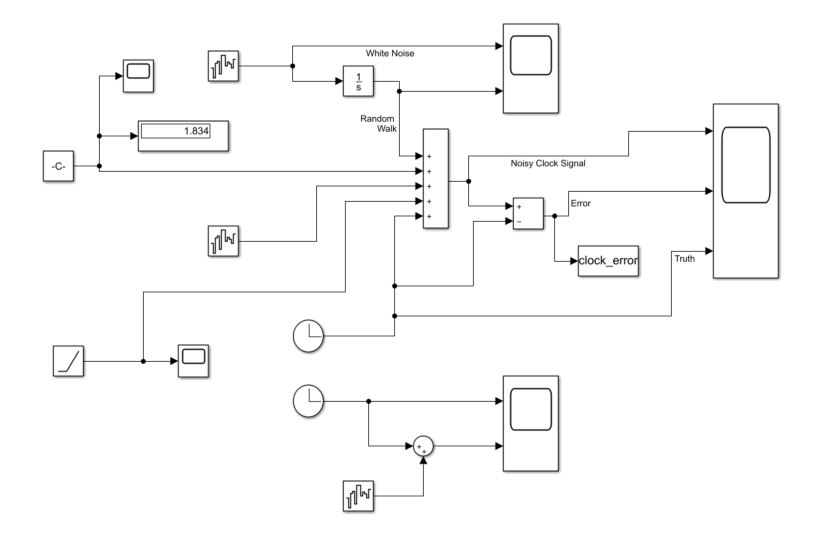
\includegraphics[scale=0.75]{day1_seg4_state_space/clock_block_diagram_model.jpg}
\onslide<1->{\center --------------------------------------------------------------------}
\end{frame}

%\begin{frame}
%missing graphic %sample_bd_01.latex
%\input{day1_seg4_state_space/sample_bd_01.latex}
\onslide<1->{\center --------------------------------------------------------------------}
%\end{frame}

% day1_seg3_state_space/deriving_state.tex
\begin{frame}
\onslide<1->{
\frametitle{Graphical Representations:  Block Diagrams}
\framesubtitle{Deriving State Equations from Block Diagrams}
}
 \begin{itemize}
 \onslide<2->{\item Continuous states can be identified as outputs of integrators
}
 \begin{itemize}
	\onslide<3->{\item First derive differential equations
}
     \onslide<4->{\item Then apply companion matrix approach to identify state dynamics matrix $A$
}
 \end{itemize}
 \onslide<5->{\item Discrete states can be identified either as sampled continous states or as outputs of delayors
}
\end{itemize}
\onslide<6->{\center --------------------------------------------------------------------}
\end{frame}

% day1_seg2_equations/examples.tex
\begin{frame}
\onslide<1->{\frametitle{Examples}
}
 \begin{itemize}
 \onslide<2->{\item Scalar Constant Dynamics
}
\onslide<3->{\item Scalar Constant Dynamics with Recursive Estimator
}
 \onslide<4->{\item Scalar Ramp Dynamics with Recursive Estimator
 \item Damped Harmonic Oscillator 
}
\end{itemize}
\onslide<5->{\center --------------------------------------------------------------------}
\end{frame}

\begin{frame}
 \onslide<1->{\frametitle{ Scalar Constant Dynamics}
}
 \begin{itemize}
 \onslide<2->{\item MATLAB/Simulink Model
}
 \onslide<3->{\item Very Simple
}
 \onslide<4->{\item Additive Noise
}
 \onslide<5->{\item No feedback loops
}
\end{itemize}
\onslide<6->{\center --------------------------------------------------------------------}
\end{frame}

\begin{frame}
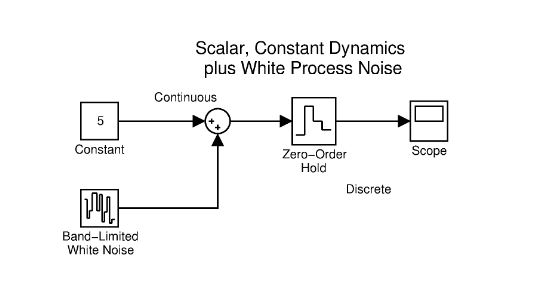
\includegraphics[scale=0.80]{matlab/scalar_const_noise.jpg}
\onslide<1->{\center --------------------------------------------------------------------}
\end{frame}

\begin{frame}
  \onslide<1->{\frametitle{Scalar Constant Dynamics with Recursive Estimator}
}
 \begin{itemize}
 \onslide<2->{\item MATLAB/Simulink Model
}
\onslide<3->{ \item Very Simple Dynamics
}
\onslide<4->{ \item Additive Noise
}
 \onslide<5->{\item Estimation loop implementing recursive simple averaging
}
 \onslide<6->{\item Simple open loop gain input
}
\end{itemize}
\onslide<7->{\center --------------------------------------------------------------------}
\end{frame}

\begin{frame}
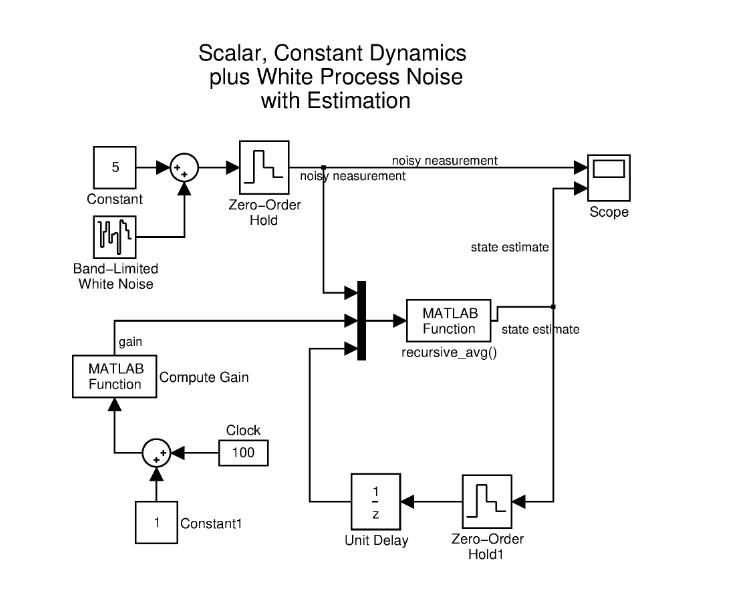
\includegraphics[scale=0.80]{day1_seg4_state_space/scalar_const_est.jpg}
\onslide<1->{\center --------------------------------------------------------------------}
\end{frame}

\begin{frame}
  \onslide<1->{\frametitle{Scalar Ramp Dynamics with Recursive Estimator}
}
 \begin{itemize}
 \onslide<2->{\item MATLAB/Simulink Model
}
 \onslide<3->{\item Scalar Dynamics with known ramp
}
 \onslide<4->{\item Additive Noise
}
 \onslide<5->{\item Estimation loop implementing recursive simple averaging
}
 \onslide<6->{\item Simple open loop gain input
}
\end{itemize}
\onslide<7->{\center --------------------------------------------------------------------}
\end{frame}

\begin{frame}
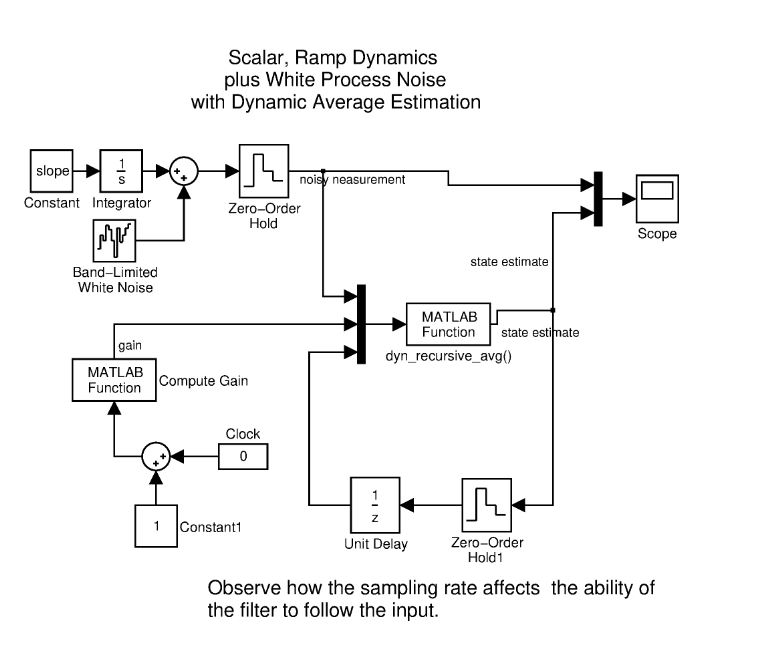
\includegraphics[scale=0.80]{matlab/scalar_ramp_noise_est.jpg}
\onslide<1->{\center --------------------------------------------------------------------}
\end{frame}

\begin{frame}
  \onslide<1->{\frametitle{Vector Dynamics: Damped Harmonic Oscillator}
}
 \begin{itemize}
 \onslide<2->{\item MATLAB/Simulink Model
}
 \onslide<3->{\item 2-dimensional Vector Dynamics
}
 \onslide<4->{\item Deterministic, Continuous Model
}
\onslide<5->{
\[
\begin{bmatrix}
\dot{x}_1\\
\dot{x}_2
\end{bmatrix} =
\begin{bmatrix}
0 & 1\\
-k/m & -c/m
\end{bmatrix}
\begin{bmatrix}
x_1\\
x_2
\end{bmatrix}
\]
}
\end{itemize}
\onslide<6->{\center --------------------------------------------------------------------}
\end{frame}

\begin{frame}
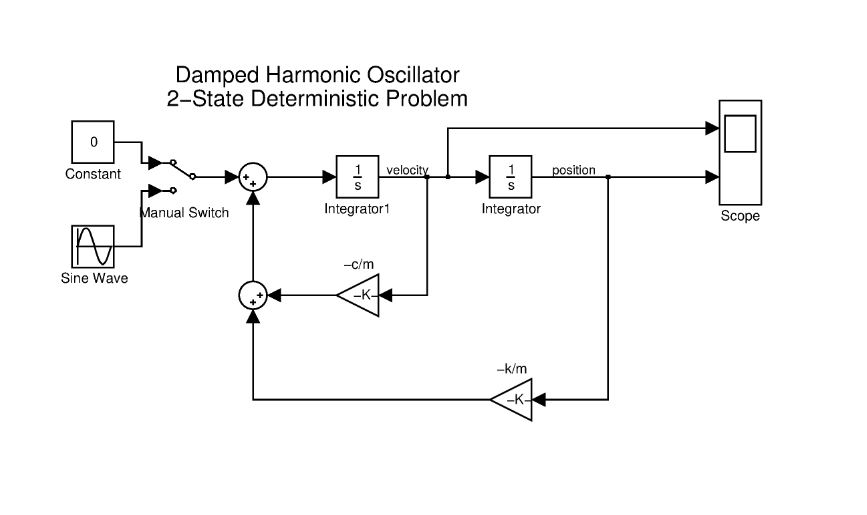
\includegraphics[scale=0.80]{day1_seg4_state_space/damped_harmosc_det.jpg}
\onslide<1->{\center --------------------------------------------------------------------}
\end{frame}

\begin{frame}
  \onslide<1->{\frametitle{Vector Dynamics: Damped Harmonic Oscillator}
}
 \begin{itemize}
 \onslide<2->{\item Discrete model would look like this}
\onslide<3->{ 
\[\begin{bmatrix}
x_{1}(k)\\
x_{2}(k)
\end{bmatrix}=\exp
\left(
\begin{bmatrix}
0 & 1\\
-k/m & -c/m
\end{bmatrix}
\Delta t
\right)
\begin{bmatrix}
x_{1}(k-1)\\
x_{2}(k-1)
\end{bmatrix}
\]
}
\onslide<3->{\item Here $\Delta t=t_k - t_{k-1}$
}
\onslide<4->{\item Note that $\exp$ is a matrix exponential
}
\onslide<5->{\item In the continuous case, the state transition matrix is a matrix exponential whenever the system dynamics matrix is a constant (i.e., time invariant) matrix
}
\end{itemize}
\onslide<6->{\center --------------------------------------------------------------------}
\end{frame}

% day1_seg3_state_space/stm.tex
\begin{frame}
\onslide<1->{\frametitle{State Transition Matrix}
}
\begin{itemize}
\onslide<2->{ 
	\item $\Phi(t,t_0)$
}
\onslide<3->{ 
	\item Needed when deriving a discrete-time state space model from a continuous-time model
 }
\onslide<4->{ 
	\item Solution of homogeneous (zero-input) equation for continuous-time systems
 }
\onslide<5->{
	\item If discrete-time system is derived from continuous-time system, then $\stmeq{k}$ satisfies:
\[
x_k=\stm{k}x_{k-1}
\]}
\end{itemize}
\onslide<6->{\center --------------------------------------------------------------------}
\end{frame}

\begin{frame}
\onslide<1->{
\frametitle{State Transition Matrix}
}
\begin{itemize}
\onslide<2->{ 
	\item $\Phi$ satisfies matrix differential equation:  $\dot{\Phi}(t,t_0)=A(t)\Phi(t,t_0)$\\
	with initial condition:  $\Phi(t_0,t_0)=I$
}
\onslide<3->{ 
	\item For a time-invariant system ($A$ is constant):  $\dot{x}(t)=Ax(t)$, solution is $\Phi(t_2,t_1)=\exp(A(t_2-t_1))$\\
}
\onslide<4->{ 
	\item For a time-varying system:  $\dot{x}(t)=A(t)x(t)$, there is NO general solution. \\
	But solutions can be found in special circumstances and several series solutions 
	are available.\\
	E.g., 	If $A(t)A(s)=A(s)A(t)$ for every pair of times $t,s$, then $\Phi(t_2,t_1)=\exp\left(\int_{t_1}^{t_2}A(\tau)d\tau\right)$

}
\end{itemize}
\onslide<5->{\center --------------------------------------------------------------------}
\end{frame}

\begin{frame}
  \onslide<1->{
	\frametitle{State Transition Matrix} 
	\framesubtitle{Properties of $\Phi$}
}
\begin{itemize}
  \onslide<2->{
\item  Transition Property: $\Phi(t_3,t_1)=\Phi(t_3,t_2)\Phi(t_2,t_1)$
}
  \onslide<3->{
\item  Inversion Property:  $\Phi^{-1}(t_2,t_1)=\Phi(t_1,t_2)$ 
}
  \onslide<4->{
	\item Separation Property:  $\Phi$ can be written as $\Phi(t_2,t_1)=\theta(t_2)\theta^{-1}(t_1)$, where $\theta$ is the solution to the matrix differential equation:\\
$\dot{\theta}(t)=A(t)\theta(t)$
}
  \onslide<5->{
	\item Determinant Property:  $\det{\Phi(t_2,t_1)}=\exp\left(\int_{t_1}^{t_2}\trace{A(\tau)}d\tau\right)$
}
\end{itemize}
\onslide<6->{\center --------------------------------------------------------------------}
\end{frame}

\begin{frame}
  \onslide<1->{
	\frametitle{State Transition Matrix} 
	\framesubtitle{Solving for $\Phi$}
}
\begin{itemize}
  \onslide<2->{
\item  Peano-Baker Series (valid even for time-varying $A(t)$):\\
$\Phi(t_2,t_1)=I+\int_{t_1}^{t_2}A(s_1)ds_1+\int_{t_1}^{t_2}A(s_1)\int_{t_1}^{s_1}A(s_2)ds_2ds_1+\cdots$
}
  \onslide<3->{
\item Another series solution is given by the Magnus series expansion involving matrix commutators  
\begin{itemize}
\item Truncated Magnus expansions exhibit many of the properties of $\Phi$
\end{itemize}
}
\end{itemize}
\onslide<4->{\center --------------------------------------------------------------------}
\end{frame}
\begin{frame}
  \onslide<1->{
	\frametitle{State Transition Matrix} 
	\framesubtitle{MATLAB Symbolic Toolbox}
}
  \onslide<2->{

syms dt;  n=8; A = zeros(n); A(1:n-1,2:n)=eye(n-1); expm(A*dt)\\
}
  \onslide<3->{
  \begin{footnotesize}
    $\Phi(t_k,t_{k-1})=\left(\begin{array}{cccccccc} 1 & \mathrm{dt} & \frac{{\mathrm{dt}}^2}{2} & \frac{{\mathrm{dt}}^3}{6} & \frac{{\mathrm{dt}}^4}{24} & \frac{{\mathrm{dt}}^5}{120} & \frac{{\mathrm{dt}}^6}{720} & \frac{{\mathrm{dt}}^7}{5040}\\ 0 & 1 & \mathrm{dt} & \frac{{\mathrm{dt}}^2}{2} & \frac{{\mathrm{dt}}^3}{6} & \frac{{\mathrm{dt}}^4}{24} & \frac{{\mathrm{dt}}^5}{120} & \frac{{\mathrm{dt}}^6}{720}\\ 0 & 0 & 1 & \mathrm{dt} & \frac{{\mathrm{dt}}^2}{2} & \frac{{\mathrm{dt}}^3}{6} & \frac{{\mathrm{dt}}^4}{24} & \frac{{\mathrm{dt}}^5}{120}\\ 0 & 0 & 0 & 1 & \mathrm{dt} & \frac{{\mathrm{dt}}^2}{2} & \frac{{\mathrm{dt}}^3}{6} & \frac{{\mathrm{dt}}^4}{24}\\ 0 & 0 & 0 & 0 & 1 & \mathrm{dt} & \frac{{\mathrm{dt}}^2}{2} & \frac{{\mathrm{dt}}^3}{6}\\ 0 & 0 & 0 & 0 & 0 & 1 & \mathrm{dt} & \frac{{\mathrm{dt}}^2}{2}\\ 0 & 0 & 0 & 0 & 0 & 0 & 1 & \mathrm{dt}\\ 0 & 0 & 0 & 0 & 0 & 0 & 0 & 1 \end{array}\right)$\\
	where $dt=t_k-t_{k-1}$
	\end{footnotesize}

  }
\onslide<4->{\center --------------------------------------------------------------------}
\end{frame}
%\begin{frame}
%  \onslide<1->{
%	\frametitle{State Transition Matrix} 
%	\framesubtitle{MATLAB Symbolic Toolbox: Companion Matrix}
%}
%\begin{tiny}
%  \onslide<2->{
%For $\left(\begin{array}{cc} 0 & 1\\ -a_{0} & -a_{1} \end{array}\right)$ 
%}
%  \onslide<3->{
%$\Phi_{11}=\frac{{\mathrm{e}}^{-\frac{\mathrm{dt}\,\sqrt{{a_{1}}^2-4\,a_{0}}}{2}-\frac{a_{1}\,\mathrm{dt}}{2}}\,\sqrt{{a_{1}}^2-4\,a_{0}}+{\mathrm{e}}^{\frac{\mathrm{dt}\,\sqrt{{a_{1}}^2-4\,a_{0}}}{2}-\frac{a_{1}\,\mathrm{dt}}{2}}\,\sqrt{{a_{1}}^2-4\,a_{0}}-a_{1}\,{\mathrm{e}}^{-\frac{\mathrm{dt}\,\sqrt{{a_{1}}^2-4\,a_{0}}}{2}-\frac{a_{1}\,\mathrm{dt}}{2}}+a_{1}\,{\mathrm{e}}^{\frac{\mathrm{dt}\,\sqrt{{a_{1}}^2-4\,a_{0}}}{2}-\frac{a_{1}\,\mathrm{dt}}{2}}}{2\,\sqrt{{a_{1}}^2-4\,a_{0}}}'$
%}
%\end{tiny}
\onslide<4->{\center --------------------------------------------------------------------}
%\end{frame}

% day1_seg3_state_space/exercises.tex
\begin{frame}
Exercises
 \begin{enumerate}
 \item Convert the differential equation
\[5\frac{d^3y}{dt^3}-0.3\frac{dy}{dt}+7y=u(t)\]
into a state space system model
 \item Convert the difference equation
\[100y(k+9) = \sum_{i=0}^2b_iu(k+2-i)\]
 \item Write the output equations for the above systems as well!
\end{enumerate}
\onslide<1->{\center --------------------------------------------------------------------}
\end{frame}


% day1_seg4_prob/probability_main.tex
\begin{frame}
  \onslide<1->{
	\frametitle{Probability and Statistics} 
	\framesubtitle{Topics}
}
\begin{itemize}
  \onslide<2->{
\item Sample Spaces and Probability Measures 
}
  \onslide<3->{
\item Probability Distributions and Densities  
}
  \onslide<4->{
\item Random Variables and Expectation  
}
  \onslide<5->{
\item Moments: Means and Variances  
}
  \onslide<6->{
\item Empirical Work: Sample Mean and Sample Variance
}
\end{itemize}
\end{frame}
% day1_seg4_prob/sample_space.tex
\begin{frame}
  \onslide<1->{
	\frametitle{Probability} 
	\framesubtitle{Sample Spaces}
}
\begin{itemize}
  \onslide<2->{
\item  Experiments 
}
  \onslide<3->{
\item Sample Space:  $\Omega$  
\begin{itemize}
 \item consists of all possible outcomes $\omega$.
 \end{itemize}
}
  \onslide<4->{
\item Events:  Subsets of $\Omega$ forming a $\sigma$-algebra.  Not necessarily \textit{all} subsets.  
}
\end{itemize}
\end{frame}

\begin{frame}
  \onslide<1->{
	\frametitle{Probability} 
	\framesubtitle{Examples:  Experiment and Sample Space}
}
\begin{itemize}
  \onslide<2->{
\item 1.  Experiment:  Single coin toss
  \begin{itemize}
  \item Sample Space:  $\Omega=\set{H,T}$
  \end{itemize}  
}
  \onslide<3->{
\item 2. Experiment:  Toss coin twice
  \begin{itemize}
  \item Sample Space:  $\Omega=\set{HH,HT,TH,TT}$
  \end{itemize}
}
\end{itemize}
\end{frame}

\begin{frame}
  \onslide<1->{
	\frametitle{Probability} 
	\framesubtitle{$\sigma$-Algebras}
}
\begin{itemize}
  \onslide<2->{
\item In probability, we are often less concerned with individual outcomes and more with sets of outcomes.  
}
  \onslide<3->{
\item Sets of outcomes, i.e., subsets of the sample space $\Omega$, are called "events".    
}
  \onslide<4->{
\item Not every subset of the sample space $\Omega$ qualifies as an event.     
}
  \onslide<5->{
\item Qualified events form an "event algebra", known in mathematics as a \textbf{$\sigma$-algebra}  
}
\end{itemize}
\end{frame}

\begin{frame}
  \onslide<1->{
	\frametitle{Probability} 
	\framesubtitle{$\sigma$-Algebras}
}
\begin{itemize}
  \onslide<2->{
\item  A $\sigma$-algebra $\mathcal{M}$ is a
 collection of subsets of $\Omega$ that is closed under arbitrary unions and
 intersections, set complementation, and which also contains the whole
 space $\Omega$ as well. 
}
  \onslide<3->{
\item A $\sigma$-algebra can be expressed in structural notation as\\
 $<\mathcal{M},\cup,\cap,\:',\emptyset,\Omega>$  
}
  \onslide<4->{
\item $\Omega$ is the certain event; $\emptyset$ is the impossible event
}
\end{itemize}
\end{frame}

\begin{frame}
  \onslide<1->{
	\frametitle{Probability} 
	\framesubtitle{Examples: $\sigma$-algebras}
}
\begin{itemize}
  \onslide<2->{
\item Double coin toss:
}
  \onslide<3->{
  \begin{itemize}
  \item Sample Space: $\Omega=\set{HH,HT,TH,TT}$
  \item $\sigma$-algebra: $\mathcal{M}=\set{\emptyset, \set{HH},\set{HT,TH,TT},\Omega}$
   \item Note that for this $\sigma$-algebra, the set $\set{TT}$ is not considered an event
  \end{itemize}  
}  
   \onslide<4->{
  \item The power set $\mathcal{P}(\Omega)$, consisting of all subsets of $\Omega$, is a $\sigma$-algebra
}
   \onslide<5->{
  \item The set consisting of just the empty set and the sample space itself is also a $\sigma$-algebra:  
  $\mathcal{M}=\set{\emptyset,\Omega}$
}
\end{itemize}
\end{frame}

\begin{frame}
  \onslide<1->{
	\frametitle{Probability} 
	\framesubtitle{Mutually Exclusive Events}
}
\begin{itemize}
  \onslide<2->{
\item Events $A,B\in\mathcal{M}$ are called \textbf{\textit{mutually exclusive}}, 
if they are disjoint as sets, i.e., if $A\cap B=\emptyset$
}
  \onslide<3->{
\item In previous example, events $\set{HH}$ and $\set{HT,TH,TT}$ are mutually exclusive
}
\end{itemize}
\end{frame}


% day1_seg4_prob/prob_measures.tex
\begin{frame}
  \onslide<1->{
	\frametitle{Probability} 
	\framesubtitle{Set Functions and Measures}
}
\begin{itemize}
  \onslide<2->{
\item A measure is a way of assigning a number to a set.  
}
  \onslide<3->{
\item Intuitively, it measures the size of the set.  
}
  \onslide<4->{
\item In probability, a measure is a way of assigning a probability to an event.  
}
\end{itemize}
\end{frame}

\begin{frame}
  \onslide<1->{
	\frametitle{Probability} 
	\framesubtitle{Set Functions and Measures}
}
\begin{itemize}
  \onslide<2->{
\item  A set function $\mu$ on $\mathcal{M}$ assigns a real number $\mu(A)$ to each set $A\in\mathcal{M}$. 
}
  \onslide<3->{
\item A set function $\mu$ on $\mathcal{M}$ is said to be \textbf{\textit{additive}}, if $\mu(A\cup B)=\mu(A)+\mu(B)$ whenever $A$ and $B$ are disjoint.  
}
  \onslide<4->{
\item $\mu$ is called \textbf{\textit{countably additive}} if $\mu(\bigcup_{i\in I}A_i)=\sum_{i\in I}\mu(A_i)$, if the family of sets $\set{A_i:i\in I}$ is disjoint.  
}
\end{itemize}
\end{frame}

\begin{frame}
  \onslide<1->{
	\frametitle{Probability} 
	\framesubtitle{Set Functions and Measures}
}
\begin{itemize}
  \onslide<2->{
\item A measure $\mu$ on a $\sigma$-algebra $\mathcal{M}$ is a real-valued, non-negative, countably additive set function:  $\mu:\mathcal{M}\rightarrow\Real$  
}
  \onslide<3->{
\item Measures are used in mathematics to define abstract integration.  
}
\end{itemize}
\end{frame}

\begin{frame}
  \onslide<1->{
	\frametitle{Probability} 
	\framesubtitle{Set Functions and Measures}
}
\begin{itemize}
  \onslide<2->{
\item Example: Counting Measure. $\Omega$ is finite and the measure of each subset is merely the number of elements in the set.  
}
  \onslide<3->{
\item Example: Dirac Measure.  Let $\mathcal{M}$ be any $\sigma$-algebra and
let $\omega\in \Omega$ be an arbitrary but fixed element of
$\Omega$. For each $A\in\mathcal{M}$ define
  \[ \mu_{\omega}(A) = \left\lbrace
  \begin{array}{c l}
    1 & \text{if $\omega\in A$},\\
    0 & \text{otherwise}.
  \end{array}
\right. \]  
}
\end{itemize}
\end{frame}

\begin{frame}
  \onslide<1->{
	\frametitle{Probability} 
	\framesubtitle{Probability Measures}
}
\begin{itemize}
  \onslide<2->{
\item A measure $\mu$ on $\mathcal{M}$ with the property 
 that $\mu(\Omega)=1$ is called a \textbf{probability measure} or \textbf{probability function}.  
}
  \onslide<3->{
\item Instead of $\mu$ we will use $P$, which is
 more customary.  
}
\end{itemize}
\end{frame}

\begin{frame}
  \onslide<1->{
	\frametitle{Probability} 
	\framesubtitle{Probability: Specialized Terminology}
}
\begin{itemize}
  \onslide<2->{
\item Null Event:  $P(A)=0$.  It is important to realize this
 does not imply that $A=\emptyset$.  In measure theory this would
 be called a set of measure zero.  
}
  \onslide<3->{
\item Independent Events:  $P(A\cap B)=P(A)P(B)$  
}
  \onslide<4->{
\item Mutually Exclusive Events: \\
 $A\cap B=\emptyset\Rightarrow P(A\cup B)=P(A)+P(B)$  
}
\end{itemize}
\end{frame}

\begin{frame}
  \onslide<1->{
	\frametitle{Probability} 
	\framesubtitle{Examples: Probability Measure}
}
\begin{itemize}
  \onslide<2->{
\item Double coin toss:  
\begin{itemize}
}  
  \onslide<3->{
\item Sample Space: $\Omega=\set{HH,HT,TH,TT}$  
}
  \onslide<4->{
\item $\sigma$-algebra: $\mathcal{M}=\set{\emptyset, \set{HH},\set{HT,TH,TT},\Omega}$  
}
  \onslide<5->{
\item Probability Measure: $P(A)=$number of elements in $A$ divided by total number of elements in $\Omega$
}
  \onslide<6->{
\item E.g., $P(\set{HH})=1/4$
}
\end{itemize}
\end{itemize}
\end{frame}
\begin{frame}
  \onslide<1->{
	\frametitle{Probability} 
	\framesubtitle{Examples: Probability Measure}
}
\begin{itemize}
  \onslide<2->{
\item Let $\Omega$ be any finite set of cardinality $n$.  Let the
 $\sigma$-algebra be the set of all subsets of $\Omega$ and let
 $|\cdot|$ denote the counting measure, i.e. for $A\subseteq\Omega$,
 $\|A|=$number of elements in $A$.  Define a probability measure
 by $P=\frac{1}{n}|\cdot|$.  
}
  \onslide<3->{
\item To illustrate the last example a little more, let
 $\Omega=\set{\omega_1,\ldots,\omega_6}$, and let
 $A=\set{\omega_1,\omega_2}$.  Then $P(A)=\frac{1}{6}\cdot|A|=\frac{1}{6}\cdot 2=\frac{1}{3}$  
}
\end{itemize}
\end{frame}
\begin{frame}
  \onslide<1->{
	\frametitle{Probability} 
	\framesubtitle{Examples: Probability Measure}
}
\begin{itemize}
  \onslide<2->{
\item Let $\Omega=[0,1]$ and let $\mathcal{B}$ be the Borel
 $\sigma$-algebra on the interval $[0,1]$.  Define $P=\lambda$,
 the Lebesgue measure on $\mathcal{B}$.  Note that for any
 open subinterval $(a,b)$ of $[a,b]$, we have $P(a,b)=b-a$.  
}
\end{itemize}
\end{frame}
\begin{frame}
  \onslide<1->{
	\frametitle{Probability} 
	\framesubtitle{Conditional Probability}
}
\begin{itemize}
  \onslide<2->{
\item Suppose you have two events $A$ and $B$ and you know that the event $B$ has in fact occured.    
}
  \onslide<3->{
\item How does that knowledge affect the probability that both $A$ and $B$ have occured?  
}
  \onslide<4->{
\item Intuitively, we would tend to think that the likelihood of $A\cap B$ increases with the knowledge that $B$ has occured.  
}
\end{itemize}
\end{frame}


\begin{frame}
  \onslide<1->{
	\frametitle{Probability} 
	\framesubtitle{Conditional Probability}
}
\begin{itemize}
  \onslide<2->{
\item The increased likelihood of $A$ given 
that $B$ has occured is called the \textbf{conditional probability} of $A$ given $B$.   
}
  \onslide<3->{
\item If $P(B)\neq 0$, then the conditional probability of $A$,
 given that $B$ has occurred, is:  $P(A|B):=P(A\cap B)/P(B)$  
}
  \onslide<4->{
\item Sometimes we say the probability of $A$ conditioned on $B$.  
}
  \onslide<5->{
\item Note that since $P(B)\leq 1$, $P(A\cap B)/P(B)\geq P(A\cap B)$  
}
\end{itemize}
\end{frame}

\begin{frame}
  \onslide<1->{
	\frametitle{Probability} 
	\framesubtitle{Conditional Probability: Bayes' Theorem}
}
\begin{itemize}
  \onslide<2->{
\item Since $P(A|B)=P(A\cap B)/P(B)$ and $P(B|A):=P(B\cap A)/P(A)$, we can eliminate $P(A\cap B)$ and derive
\[P(A|B)=\dfrac{P(B|A)P(A)}{P(B)}\]  
}
  \onslide<3->{
\item Using this we obtain Bayes' Theorem (simple form):
\begin{equation}\label{bayes}
   P(A|B)=\frac{P(A)P(B|A)}{P(A)P(B|A)+P(A')P(B|A')}.
\end{equation}  
}
\end{itemize}
\end{frame}

\begin{frame}
  \onslide<1->{
	\frametitle{Probability} 
	\framesubtitle{Conditional Probability}
}
\begin{itemize}
  \onslide<2->{
\item Bayes' Theorem (complex form):  Let $A_1,\ldots,A_n$ be a
 partition of $\Omega$.  Then,
\begin{equation}\label{bayescomplex}
   P(A_i|B)=\frac{P(A_i)P(B|A_i)}{\sum_{j=1}^{n}P(A_j)P(B|A_j)}.
\end{equation}  
}
  \onslide<3->{
\item Bayes' Theorem expresses posterior probability in terms of
 prior probabilities and conditional probabilities.  
}
\end{itemize}
\end{frame}
\begin{frame}
  \onslide<1->{
	\frametitle{Probability} 
	\framesubtitle{Conditional Probability}
}
\begin{itemize}
  \onslide<2->{
\item In one derivation of the Kalman filter, the use of Bayes'
 Theorem is a crucial step.  We'll see this later.  
}
  \onslide<3->{
\item Bayes' Theorem is used to derive the Kalman gain: to
 determine the best estimate of state \textbf{after} measurement has
 occurred.  
}
\end{itemize}
\end{frame}

\begin{frame}
  \onslide<1->{
	\frametitle{Probability} 
	\framesubtitle{Conditional Probability}
}
\begin{itemize}
  \onslide<2->{
\item Bayes' Theorem allows us to reverse the conditional probability.  
}
  \onslide<3->{
\item We can derive information about the state conditioned on the measurement from 
information about the measurement conditioned on the state.    
}
\end{itemize}
\end{frame}

\begin{frame}
	\onslide<1->{
	\frametitle{Statistics} 
	\framesubtitle{Random Variables}
}
\begin{itemize}
  \onslide<2->{
\item In measure-theoretic terms, a ra\textbf{ndom variable} 
is simply a real-valued measurable function on the sample space $\Omega$.   
}
  \onslide<3->{
\item A \textbf{measurable function} is one such that the inverse image of any 
open set in $\Real$ is measurable (i.e. is a member of the $\sigma$-algebra).   
}
  \onslide<4->{
\item Some elementary probability texts are not that strict and instead consider 
any real-valued function of the sample space to be a random variable.  
}
\end{itemize}
\end{frame}

\begin{frame}
  \onslide<1->{
	\frametitle{Statistics} 
	\framesubtitle{Random Variables}
}
\begin{itemize}
  \onslide<2->{
\item We use capital letters at the end of the alphabet to denote random variables:  $X,Y,Z, ...$ 
(This helps us distinguish them from ordinary real-valued variables.)  
}
  \onslide<3->{
\item Later we will use lowercase letters so as not to confuse them with certain transforms.  
}
\end{itemize}
\end{frame}
\begin{frame}
  \onslide<1->{
	\frametitle{Statistics} 
	\framesubtitle{Random Variables}
}
\begin{itemize}
  \onslide<2->{
\item Note that random variables are not really variables in any ordinary sense -- they are functions.  Thus, if $\omega\in \Omega$, and $X$ is a random 
variable on $\Omega$, then $X(\omega)\in\Real$, i.e., $X(\omega)$ is a real number.  
}
  \onslide<3->{
\item Also note that $X^{-1}(A)=\set{\omega\in\Omega | X(\omega)\in A}$ is 
always an event in the event algebra by definition.  
}
\end{itemize}
\end{frame}
\begin{frame}
  \onslide<1->{
	\frametitle{Statistics} 
	\framesubtitle{Random Variables}
}
\begin{itemize}
  \onslide<2->{
\item Random variables provide a way to quantify the outcomes of
 experiments  
}
  \onslide<3->{
\item Random variables are important because we are often more
 interested in the consequences of an experiment than in the
 experiment itself  
}
  \onslide<4->{
\item For example, a gambler is usually more interested in his
 wins and losses than in the particular game he's playing  
}
\end{itemize}
\end{frame}
\begin{frame}
  \onslide<1->{
	\frametitle{Statistics} 
	\framesubtitle{Random Variables}
}
\begin{itemize}
  \onslide<2->{
\item Moreover, random variables are not really random  
}
  \onslide<3->{
\item They are deterministic functions from the space of all possible outcomes
 to the real numbers.  If you give them a particular outcome to operate on,
 they return the same real value every time.  
}
  \onslide<4->{
\item What gives them the appearance of randomness is really the fact that you don't 
really know what those values are.  Usually, 
you only know (or assume you know) certain statistical properties like 
distributions (to be discussed soon).  
}
\end{itemize}
\end{frame}
\begin{frame}
  \onslide<1->{
	\frametitle{Statistics} 
	\framesubtitle{Random Variables}
}
\begin{itemize}
  \onslide<2->{
\item The "randomness" of random variables stems from the
 probabilistic nature of the underlying sample space.  Usually, we
 can't say much about the individual outcomes in a sample space.
 We can only measure the size of events. (The connection between the
 "randomness" of the underlying space and the random variables will
 be made by means of probability distributions.)  
}
  \onslide<3->{
\item It is because random variables are functions that we find
 ourselves having to deal with infinite dimensional vector
 spaces, i.e., function spaces.  
}
\end{itemize}
\end{frame}
\begin{frame}
  \onslide<1->{
	\frametitle{Statistics} 
	\framesubtitle{Equality and Equivalence of Random Variables}
}
\begin{itemize}
  \onslide<2->{
\item Since random variables are functions, strict equality of
 random variables is the same as the equality of functions.  Two
 functions are equal if and only if they have equal values when
 evaluated at the same point:  $X=Y\Leftrightarrow
 X(\omega)=Y(\omega)$ for all $\omega\in\Omega$.  
}
  \onslide<3->{
\item However, when you take probability into account, things can
 get a little fuzzier.  We say that two random variables $X$ and
 $Y$ are equal \textit{\textbf{almost surely}} (a.s.) if $P\set{\omega\in\Omega:X(\omega)\neq
 Y(\omega)}=0$.  
}
  \onslide<4->{
\item In other words, $X=Y \text{a.s.}$, if the set of all points at
 which $X$ and $Y$ differ is insignificant, i.e., of measure 0.  
}
\end{itemize}
\end{frame}
\begin{frame}
  \onslide<1->{
	\frametitle{Statistics} 
	\framesubtitle{Simple Random Variables}
}
\begin{itemize}
  \onslide<2->{
\item If a random variable $X$ takes on only finitely many
 values, then $X$ is called a \textit{\textbf{simple random variable}}.
 \item If $X$ is a simple random variable and
 $\set{a_1,\cdots,a_n}$ are its values, let $A_i=\set{\omega:X(\omega)=a_i}$
 for each $i=1,\ldots,n$.\\  
}
  \onslide<3->{
Then $X$ can bewritten as a
 sum:
\begin{equation}\label{simple_rv}
  X=\sum_{i=1}^{n}a_i\chi_{A_i}
\end{equation}
where $\chi_{A_i}$ is the characteristic or indicator function on $A_i$ defined by\\
 $\chi_{A_i}(\omega)=
  \begin{cases}
    1 & \text{if } \omega\in A_i, \\
    0 & \text{otherwise}.
  \end{cases}$
}
\end{itemize}
\end{frame}

\begin{frame}
  \onslide<1->{
	\frametitle{Statistics} 
	\framesubtitle{Example:  Simple Random Variable}
}
\begin{itemize}
  \onslide<2->{
\item Double coin toss:  
}
  \onslide<3->{
  \begin{itemize}
  \item Sample Space: $\Omega=\set{HH,HT,TH,TT}$
}
  \onslide<4->{
\item $\sigma$-algebra: $\mathcal{M}=\set{\emptyset, \set{HH},\set{HT,TH,TT},\Omega}$  
}
  \onslide<5->{
\item Probability Measure: $P(A)=$number of elements in $A$ divided by total number of elements in $\Omega$
\end{itemize}  
}
\end{itemize}
\end{frame}

\begin{frame}
  \onslide<1->{
	\frametitle{Statistics} 
	\framesubtitle{Example:  Simple Random Variable}
}
\begin{itemize}
  \onslide<2->{
\item Let $A=\set{HT,TH,TT}$ and define $X=\chi_A$.  Then
\begin{align*}
X(HH)&=0\\
X(HT)&=1\\
X(TH)&=1\\
X(TT)&=1
\end{align*}  
}
\end{itemize}
\end{frame}

\begin{frame}
  \onslide<1->{
	\frametitle{Statistics} 
	\framesubtitle{Example:  Simple Random Variable}
}
\begin{itemize}
  \onslide<2->{
\item Let $B=\set{HH}$ and define $Y=-3\chi_A + 0.5\chi_B$  
}
  \onslide<3->{
\item $Y$ is a simple random variable.  
}
  \onslide<4->{
\item We compute:  
\begin{align*}
  Y(HH)&=-3\chi_A(HH) + 0.5\chi_B(HH)\\
&=-3\cdot 0 + 0.5\cdot 1\\
&=0.5
\end{align*}
}
\end{itemize}
\end{frame}

\begin{frame}
  \onslide<1->{
	\frametitle{Statistics} 
	\framesubtitle{Random Variables form a Vector Space}
}
\begin{itemize}
  \onslide<2->{
\item Let $RV(\Omega)$ denote the set of all random variables on $\Omega$.
 If $X,Y\in RV(\Omega)$ and $a,b\in \Real$, then $aX+bY\in
 RV(\Omega)$.  
}
  \onslide<3->{
\item Scalar multiplication:  Recall that $(aX+bY)(\omega):=a\cdot X(\omega)+b\cdot
 Y(\omega)$, where $\cdot$ denotes ordinary real multiplication.
 }
   \onslide<4->{
 \item For brevity we will drop the $\cdot$ and merely
 juxtapose.  Likewise, we will drop $\Omega$ from $RV(\Omega)$
 and merely write $RV$, assuming implicitly that the underlying sample space is
 $\Omega$. 
}
  \onslide<5->{
  \item Thus, $RV(\Omega)$ becomes a vector space over the reals.  It is an infinite dimensional vector space.\\
  In fact, after we define a norm and inner products on $RV(\Omega)$ using statistical expectation, 
  we will see that it becomes a Hilbert space (modulo almost surely equivalence).
  }
\end{itemize}
\end{frame}

% day1_seg4_prob/prob_dist.tex
\begin{frame}
  \onslide<1->{
	\frametitle{Statistics} 
	\framesubtitle{Probability Distributions and Densities}
}
\begin{itemize}
  \onslide<2->{
\item Probability Distributions  
}
  \onslide<3->{
\item Probability Density Functions  
}
\end{itemize}
\end{frame}

\begin{frame}
  \onslide<1->{
	\frametitle{Statistics} 
	\framesubtitle{Probability Distributions}
}
\begin{itemize}
  \onslide<2->{
 \item Every random variable $X$ has an associated probability \textbf{\textit{distribution}} function
 defined by
\[F_X(x)=P\{X^{-1}[-\infty,x)\}=P\set{\omega\in\Omega:X(\omega)< x}\]\\
Also referred to as a \textbf{\textit{Cumulative Distribution Function (c.d.f.)}}
}
  \onslide<3->{
 \item The value of the distribution function at a real number $x$ is the
 probability that the value of $X$ does not exceed $x$.
}
  \onslide<4->{
 \item We can simplify the notation by writing $\set{X< x}$
 instead of $\set{\omega\in\Omega : X(\omega)< x}$.
}
  \onslide<5->{
 \item Thus, $F_X(x)=P\set{X< x}$.
}
\end{itemize}
\end{frame}

\begin{frame}
  \onslide<1->{
	\frametitle{Statistics} 
	\framesubtitle{Probability Distributions}
}
\begin{itemize}
  \onslide<2->{
 \item Distributions are nondecreasing:  $x\leq y\Rightarrow F(x)\leq
 F(y)$.
}
  \onslide<3->{
 \item Distributions are always continuous from the left:  \\
 $F(x)\rightarrow F(a)$ as $x\uparrow a$.
}
  \onslide<4->{
 \item The value of a distribution is always between 0 and 1
 inclusively, and $\lim_{x\downarrow -\infty}F(x)=0$ and $\lim_{x\uparrow \infty}F(x)=1$
}
\end{itemize}
\end{frame}

\begin{frame}
  \onslide<1->{
	\frametitle{Statistics} 
	\framesubtitle{Probability Distributions: Three Flavors}
}
\begin{itemize}
  \onslide<2->{
\item Continuous (no jumps)
 }
  \onslide<3->{
 \item Piecewise continuous (some jumps)
}
  \onslide<4->{
 \item Discrete (only jumps and flat).  $X$ is discrete if and only if $X$
 takes on only finitely many, or at most countably infinite,
 distinct values.  Note that a simple measurable function is a
 discrete random variable.
}
\end{itemize}
\end{frame}

\begin{frame}
  \onslide<1->{
	\frametitle{Statistics} 
	\framesubtitle{Some Discrete Distributions}
}
\begin{itemize}
  \onslide<2->{
 \item Discrete Uniform Distribution:  Let $A=\set{a_1,\ldots,a_n}$ be a set of $n$ distinct real numbers and assume that $a_1<a_2<\ldots<a_n$.  
 Then a random variable $X$ is said to have a discrete uniform
 distribution if \\
 $F(x)= \frac{1}{n}\cdot \abs{A\cap [-\infty, x)}$.
}
  \onslide<3->{
 \item Let $\Omega$ be any sample space and $A\subseteq \Omega$.
 Let $X(\omega)=\chi_A(\omega)$.  Recall that
 $\chi_A(\omega)=
  \begin{cases}
    1 & \text{if } \omega\in A, \\
    0 & \text{otherwise}.
  \end{cases}
$ \\
Then $F(x)=
  \begin{cases}
    0   & \text{if } x<0, \\
    1-P(A) & \text{if } 0\leq x<1, \\
    1   &  \text{if } x\geq 1.
  \end{cases}
$
}
\end{itemize}
\end{frame}

\begin{frame}
  \onslide<1->{
	\frametitle{Statistics} 
	\framesubtitle{Continuous Distributions:  Probability Density Functions}
}
\begin{itemize}
  \onslide<2->{
 \item $X$ is said to have a continuous distribution if there
 exists a function $f:\Real\rightarrow \Real$ such that for each
 $x\in \Real$ \\
\begin{equation}\label{pdf1}
   F(x)=\int_{-\infty}^{x}f(u)du.
\end{equation}
}
  \onslide<3->{
 \item $f$ is called a \textit{\textbf{probability density
 function}}, or p.d.f, for short.
 \item The p.d.f of a random variable, if it exists, is not
 unique.  Why?
}
\end{itemize}
\end{frame}

\begin{frame}
  \onslide<1->{
	\frametitle{Statistics} 
	\framesubtitle{Some Important Distributions}
}
\begin{itemize}
  \onslide<2->{
 \item The Gaussian or normal distribution with p.d.f:
\begin{equation}\label{gauss_distr}
 f(x)=\frac{1}{\sigma\sqrt{2\pi}}\exp\left[-\frac{(x-\mu)^2}{2\sigma^2}\right]
\end{equation}
}
  \onslide<3->{
 \item The uniform distribution on $[a,b]$ with distribution function:
\begin{equation}\label{uniform_distr}
  F(x)=
  \begin{cases}
    0 & \text{if } x< a, \\
    \frac{x-a}{b-a} & \text{if } a\leq x< b,\\
    1 & \text{otherwise}.
  \end{cases}
\end{equation}
}
\end{itemize}
\end{frame}

% day1_seg4_prob/moments.tex
\begin{frame}
  \onslide<1->{
	\frametitle{Statistics} 
	\framesubtitle{Moments: Means and Variances of Random Variables}
}
\begin{itemize}
  \onslide<2->{
\item 1st Order Moment: Expectation or Mean  
}
  \onslide<3->{
\item  2nd Order Moment: Variance 
}
  \onslide<4->{
\item Higher Order Moments  
}
\end{itemize}
\end{frame}
\begin{frame}
  \onslide<1->{
	\frametitle{Statistics} 
	\framesubtitle{1st Order Moment: Expectation of a Random Variable}
}
\begin{itemize}
  \onslide<2->{
 \item Let $X$ be a simple random variable and let
 $a_1,\ldots,a_n$ be the distinct values taken on by $X$.  Then,
 the expectation operator $\text{E}:SRV\rightarrow \Real$ is defined as
\begin{equation}\label{simp_expect}
  \expect{X}=\sum_{i=1}^{n}a_iP(A_i)
\end{equation}
where $A_i=X^{-1}\set{a_i}=\set{\omega\in\Omega:X(\omega)=a_i}$.
}
  \onslide<3->{
 \item Thus, the expectation of $X$ is the weighted
 sum of the values of $X$, the weights being the "size" or likelihood
 of the events.
}
  \onslide<4->{
 \item It is clear that $X=Y \text{a.s.}\Rightarrow
 \expect{X}=\expect{Y}$.
}
\end{itemize}
\end{frame}
\begin{frame}
  \onslide<1->{
	\frametitle{Statistics} 
	\framesubtitle{Expectation}
}
\begin{itemize}
  \onslide<2->{
 \item Alternative Integral notation:
$\expect{X}=\int_{\Omega}XdP$, because the weighted sum given in
\ref{simp_expect} is just the definition of the integral of $X$
with respect to the (probability) measure $P$.
}
  \onslide<3->{
 \item It can be shown that every random variable $X$ can be
 written as the difference of two nonnegative random variables.
}
  \onslide<4->{
 \item It can also be shown that every nonnegative random variable
 is the limit of a monotone sequence of simple random variables.
 Therefore, integration can be extended from $SRV(\Omega)$ to $RV(\Omega)$
}
\end{itemize}
\end{frame}

\begin{frame}
  \onslide<1->{
	\frametitle{Statistics} 
	\framesubtitle{Expectation}
}
\begin{itemize}
  \onslide<2->{
  \item Note that we did not need the use of a probability distribution nor density in defining the expectation this way.
}
  \onslide<3->{
  \item We only needed the probability function.
}
  \onslide<4->{
  \item Note also that the integration we defined above is abstract in the  sense that it works just as well for general measures, not just probability measures.
}
\end{itemize}
\end{frame}

\begin{frame}
  \onslide<1->{
	\frametitle{Statistics} 
	\framesubtitle{Expectation}
}
\begin{itemize}
  \onslide<2->{
 \item Expectation is a linear functional on the space $RV$ of random variables over $\Omega$:
 \[\expect{aX+bY}=a\expect{X}+b\expect{Y}\]
}
  \onslide<3->{
 \item Expectation is monotonic:
 \[X\leq Y a.s.\Rightarrow \expect{X}\leq \expect{Y}\]
}
  \onslide<4->{
 \item We can compute $\expect{X}$ by means of an ordinary
 Riemann-Stieltjes integral:
}
  \onslide<5->{
\begin{equation}\label{expect-RS}
  \expect{X}= \infint xdF(x)
\end{equation}
}
\end{itemize}
\end{frame}

\begin{frame}
  \onslide<1->{
	\frametitle{Statistics} 
	\framesubtitle{Expectation}
}
\begin{itemize}
  \onslide<2->{
 \item If $X$ also has a p.d.f, then equation \eqref{expect-RS}
 becomes:
\begin{equation}\label{expect-pdf}
  \expect{X} = \infint xdF(x) = \infint xF'(x)dx = \infint xf(x)dx
\end{equation}
}
  \onslide<3->{
 \item The expectation of $\exp(juX)$ for each $u\in \Real$ is
 called the \textit{\textbf{characteristic function}} of $X$:
\begin{equation}\label{charfunc}
  \phi_X(u)=\expect{\exp(juX)} = \infint \exp(jux)dF(x)
\end{equation}
where $j=\sqrt{-1}$.
}
\end{itemize}
\end{frame}
\begin{frame}
  \onslide<1->{
	\frametitle{Statistics} 
	\framesubtitle{2nd order moment:  Variance}
}
\begin{itemize}
  \onslide<2->{
 \item The variance of a random variable is defined as the mean square deviation from the mean:
\[\sigma^2 = \expect{(X-\mu)^2}\]
}
\end{itemize}
\end{frame}
\begin{frame}
  \onslide<1->{
	\frametitle{Statistics} 
	\framesubtitle{Higher Order Moments}
}
\begin{itemize}
  \onslide<2->{
 \item The value of the integral
 \[m_i=\infint x^nf(x)dx\]
 is called the $n^{th}$ \textit{\textbf{moment}} of the distribution.  If instead we
 subtract out the mean $\mu=\expect{X}$ prior to integrating, then we obtain the $n^{th}$
 \textit{\textbf{central moment}}:
 \[\mu_i=\infint (x-\mu)^nf(x)dx \]
}
  \onslide<3->{
 \item We note that $\mu=\mu_1$, the first order moment, or mean
}
\end{itemize}
\end{frame}
\begin{frame}
  \onslide<1->{
	\frametitle{Statistics} 
	\framesubtitle{Higher Order Moments}
}
\begin{itemize}
  \onslide<2->{
 \item The characteristic function $\phi_X$ is similar to the \textit{\textbf{moment generating
 function}} defined as follows:
\[M_X(t)=\expect{\exp(tX)}\]
}
  \onslide<3->{
 \item If $X$ has a density function $f$, then
 \[M_X(t)=\infint \exp(tx)f(x)dx\]
}
\end{itemize}
\end{frame}

\begin{frame}
  \onslide<1->{
	\frametitle{Statistics} 
	\framesubtitle{Higher Order Moments}
}
\begin{itemize}
  \onslide<2->{
 \item Note that
 \[\mu=\expect{X}=\frac{d}{dx}M_X(0)\]
  and, in general,
  \[\expect{X^n}=\frac{d^n}{dx^n}M_X(0).\]
}
  \onslide<3->{
 \item The Gaussian distribution has only two fundamental moments $\mu=\expect{X}$ and
 $\sigma^2=\expect{(X-\mu)^2}$.  All higher-order moments can be
 expressed in terms of these two.
}
  \onslide<4->{
 \item Thus, the Gaussian distribution is said to be a second-order distribution.
}
\end{itemize}
\end{frame}
\begin{frame}
  \onslide<1->{
	\frametitle{Statistics} 
	\framesubtitle{Covariance and Correlation Between Random Variables}
}
\begin{itemize}
  \onslide<2->{
\item  Let $X$ and $Y$ be two different random variables, 
i.e., functions from the sample space $\Omega$ into the reals $\Real$. 
}
  \onslide<3->{
\item Let $\sigsq{X}=\variance{X}$ be the variance of $X$ and $\sigsq{Y}=\variance{Y}$ be the variance of $Y$, 
and let $\mu_X,\mu_Y$ be their respective means.   
}
  \onslide<4->{
\item The \textbf{covariance} between $X$ and $Y$ is the mean of their product, 
after removing their means: $\covdef{X}{Y}$ 
}
  \onslide<5->{
\item Their correlation is their covariance normalized by the product of their standard deviations:
$\corrdef{X}{Y}$
}
\end{itemize}
\end{frame}



% empirical stats:  empirical_stats.tex
\begin{frame}
  \onslide<1->{
	\frametitle{Empirical Statistics} 
	\framesubtitle{Sample Means, Variances, etc.}
}
\begin{itemize}
  \onslide<2->{
\item Previously defined quantities $\mu_X,\sigma_X,\ldots$ were all theoretical properties, sometimes referred to 
as population statistics  
}
  \onslide<3->{
\item With real data we rarely know the true statistics;  we only have sampled data to go on  
}
  \onslide<4->{
\item But we can define quantities analogous to $\mu_X,\sigma_X,\ldots$ that we can actually compute 
using real data and that are generally in some sense approximations to the true values
}
\end{itemize}
\end{frame}
\begin{frame}
  \onslide<1->{
	\frametitle{Empirical Statistics} 
	\framesubtitle{Sample Means, Variances, etc.}
}
\begin{footnotesize}
\begin{itemize}
  \onslide<2->{
\item   With $N$ samples of random variable $X$, the \textbf{Sample Mean} is:  $$\samplemeandef{X}$$
}
  \onslide<3->{
\item The \textbf{Sample Variance} is: $$\samplevardef{X}$$  
}
  \onslide<4->{
\item  The \textbf{Sample Covariance} is: $$\samplecovdef{X}{Y}$$ 
}
  \onslide<5->{
\item   The \textbf{Sample Correlation} is: $$\samplecorrdef{X}{Y}$$
}
\end{itemize}
\end{footnotesize}
\end{frame}
\begin{frame}
  \onslide<1->{
	\frametitle{Empirical Statistics} 
	\framesubtitle{Sample Stats with MATLAB}
}
\begin{footnotesize}
True $\mu,\sigma$: mu=30;sigma=10;\\
1,000 samples:  X=mu+sigma*randn(1000,1);\\
$\samplemean{X}=29.6737$ and $\samplevar{X}=99.7932$ (sample standard deviation $s_X=9.9897$)\\
\begin{center}
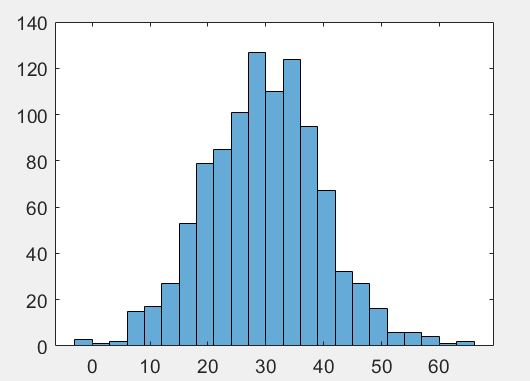
\includegraphics[scale=0.80]{day2_seg1_prob/histogram.jpg}
\end{center}
\end{footnotesize}
\end{frame}

\begin{frame}
  \onslide<1->{
	\frametitle{Empirical Statistics} 
	\framesubtitle{Sample Stats with MATLAB}
}
\begin{footnotesize}
True $\mu,\sigma$: mu=30;sigma=10;\\
10,000 samples: X=mu+sigma*\text{randn}(10000,1);\\
$\samplemean{X}=30.0563$ and $\samplevar{X}=97.3913$ (sample standard deviation $s_X=9.8687$)\\
\begin{center}
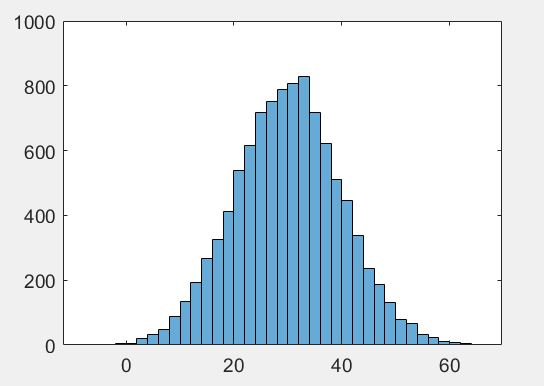
\includegraphics[scale=0.80]{day2_seg1_prob/histogram10000.jpg}
\end{center}
\end{footnotesize}
\end{frame}

\begin{frame}
  \onslide<1->{
	\frametitle{Empirical Statistics} 
	\framesubtitle{Sample Stats with MATLAB}
}
\begin{footnotesize}
True $\mu,\sigma$: mu=30;sigma=10;\\
10,000 samples: X=mu+sigma*\text{randn}(10000,1);\\
$\samplemean{X}=30.0563$ and $\samplevar{X}=97.3913$ (sample standard deviation $s_X=9.8687$)\\
\begin{center}
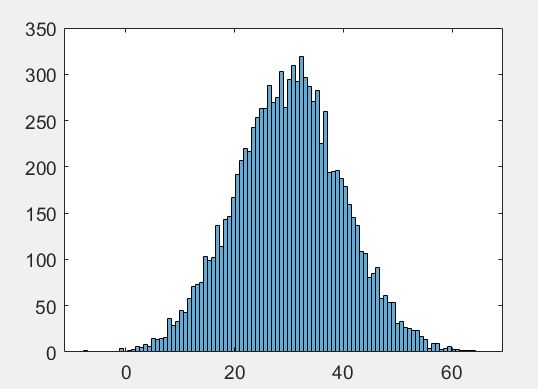
\includegraphics[scale=0.80]{day2_seg1_prob/histogram10000more_bins.jpg}
\end{center}
\end{footnotesize}
\end{frame}

\begin{frame}
  \onslide<1->{
	\frametitle{Empirical Statistics} 
	\framesubtitle{Sample Stats with MATLAB}
}
\begin{footnotesize}
True $\mu,\sigma$: mu=30;sigma=10;\\
10,000 samples: X=mu+sigma*randn(10000,1);\\
$\samplemean{X}=30.0563$ and $\samplevar{X}=97.3913$ (sample standard deviation $s_X=9.8687$)\\
$\;\;\;$\\
Define new random variable $Y$ to be linearly dependent on $X$ plus 
some random Gaussian noise:Y=3*X+2+randn(10000,1);\\
$\;\;\;$\\
MATLAB's corrcoef functions says (rightly) that $X$ and $Y$ are highly correlated: $r_{XY}=0.9994$
\end{footnotesize}
\end{frame}

% day1_seg4_prob/exercises.tex
\begin{frame}
  \onslide<1->{
	\frametitle{Probability and Statistics} 
	\framesubtitle{Exercises}
}
\begin{itemize}
  \onslide<2->{
 \item Show that $A\subseteq B\Rightarrow P(A)\leq P(B)$.\\
 (Hint: Use $B=A\cup (B\setminus A)$ and the fact that measures are additive.)
}
  \onslide<3->{
 \item Show that $P(A\cup B)=P(A)+P(B)-P(A\cap B)$
}
  \onslide<4->{
 \item Let $F$ be the distribution of a random variable $X$
 and suppose that $a\leq b$ are real numbers.  Show
 that $P(x\in [a,b))=F(b)-F(a)$.
}
\end{itemize}
\end{frame}
\begin{frame}
  \onslide<1->{
	\frametitle{Probabillity and Statistics} 
	\framesubtitle{Exercises}
}
\begin{itemize}
  \onslide<2->{
 \item Prove the following:  If two events $A$ and $B$ are
 independent, then the events $A$ and $B'$ are also independent.
}
  \onslide<3->{
 \item Show that for any distribution function $F$ of a random variable $X$,
  $P(X>a)=\lim_{x\downarrow a} F(x)$.
}
\end{itemize}
\end{frame}

\begin{frame}
  \onslide<1->{
	\frametitle{Statistics} 
	\framesubtitle{Exercises}
}
\begin{itemize}
  \onslide<2->{
 \item Let $\Omega$ be any sample space and $A\subseteq \Omega$.
  Let $X(\omega)=\chi_A(\omega)$.  Recall that
 $\chi_A(\omega)=
  \begin{cases}
    1 & \text{if } \omega\in A, \\
    0 & \text{otherwise}.
  \end{cases}$ \\
 Prove that
 $F(x)=
  \begin{cases}
    0   & \text{if } x<0, \\
    1-P(A) & \text{if } 0\leq x<1, \\
    1   &  \text{if } x\geq 1.
  \end{cases}$
}
\end{itemize}
\end{frame}

\begin{frame}
  \onslide<1->{
	\frametitle{Probability and Statistics} 
	\framesubtitle{Exercises}
}
\begin{itemize}
  \onslide<2->{
 \item A gyro manufacturer produces defective gyros with
 probability $p$, where $0<p<1$.  After a lot of $n$ independent
 gyros have been produced, they are
 examined.  Let $X$ denote the number of defective gyros in the
 lot.  What is the probability mass function of this discrete
 distribution?
}
\end{itemize}
\end{frame}



% day2_seg1_ranproc1/ranproc_main.tex
\begin{frame}
  \onslide<1->{
	\frametitle{Random Processes} 
	\framesubtitle{Topics}
}
\begin{itemize}
  \onslide<2->{
 \item Two Dimensions:  Ensemble vs. Time
}
  \onslide<3->{
 \item Stationary and Ergodic
}
  \onslide<4->{
 \item Correlation and Covariance
}
  \onslide<5->{
 \item Power Spectral Density
}
\end{itemize}
\end{frame}
% day2_seg1_ranproc1/twodim.tex


\begin{frame}
  \onslide<1->{
	\frametitle{Random Processes} 
	\framesubtitle{Two Dimensions:  Ensemble vs. Time}
}
\begin{itemize}
  \onslide<2->{
 \item Two equivalent ways to define a random process:  
 One way views a random process as a time function whose value at each 
 instant of time is a random variable.
}
  \onslide<3->{
 \item The other defines a random process as a function of two variables: 
 the outcomes $\omega\in\Omega$ and time $t$.  
}
  \onslide<4->{
 \item Outcomes $\omega$ belong to sample space $\Omega$ while times $t$ are represented as real numbers, 
 often non-negative.
}
\end{itemize}
\end{frame}

\begin{frame}
  \onslide<1->{
	\frametitle{Random Processes} 
	\framesubtitle{Two Dimensions:  Ensemble vs. Time}
}
\begin{itemize}
  \onslide<2->{
 \item At each fixed $t$, the random process $X(\cdot,t)$, or simply $X(t)$ is simply a random variable, 
 i.e., a function of the other variable $\omega$ alone
}
  \onslide<3->{
 \item For a fixed $\omega$, we have an ordinary time function of $t$.
}
\end{itemize}
\end{frame}


\begin{frame}
  \onslide<1->{
	\frametitle{Random Processes} 
	\framesubtitle{Definitions}
}
\begin{itemize}
  \onslide<2->{
 \item A \textit{\textbf{Random Process}} (also called a \textit{\textbf{stochastic process}}) is a
 function $X:[0,T]\rightarrow RV(\Omega)$, where $[0,T]$ is a
 closed interval of the real line.
}
  \onslide<3->{
 \item We think of variables $t\in [0,T]$ as time.
}
  \onslide<4->{
 \item The image of $t\in [0,T]$ under $X$ is a random variable:
 \[X(t):\Omega\rightarrow \Real\].
}
 \onslide<5->{
   \item The random variables $X(s)$ and $X(t)$ are not necessarily correlated in any way (when $x\neq t$)
 }
\end{itemize}
\end{frame}

\begin{frame}
  \onslide<1->{
	\frametitle{Random Processes} 
	\framesubtitle{Curves in Hilbert Space}
}
\begin{itemize}
  \onslide<2->{
 \item Thus a random process can be viewed as a function whose values are
 themselves functions
}
  \onslide<3->{
 \item We could also think of $X$ as a two-variable function from the Cartesian product 
 $[0,T]\times \Omega$ into the reals:
 \[X(t,\omega)\in \Real\]
}
\end{itemize}
\end{frame}

\begin{frame}
  \onslide<1->{
	\frametitle{Random Processes} 
	\framesubtitle{}
}
\begin{itemize}
  \onslide<2->{
 \item These two perspectives are interchangeable and we shall use
 both.
}
  \onslide<3->{
 \item We use all of the following notation for a random process 
\[X_t\]
\[X_t(\omega)\]
\[X(t)\]
\[X(t,\omega)\] 
}
\end{itemize}
\end{frame}


\begin{frame}
  \onslide<1->{
	\frametitle{Random Processes} 
	\framesubtitle{}
}
\begin{itemize}
  \onslide<2->{
 \item If you fix $\omega$ and let $t$ vary you get a \textit{\textbf{sample
 trajectory}}.
}
  \onslide<3->{
 \item In this way, you can think of $X$ as an ensemble of sample
 trajectories.
}
  \onslide<4->{
 \item Therefore, we will talk about both sample trajectory
 properties (continuity, differentiability, etc.) and ensemble
  properties (statistical).
}
\end{itemize}
\end{frame}

\begin{frame}
  \onslide<1->{
	\frametitle{Random Processes} 
	\framesubtitle{Random Process as Ensemble of Trajectories}
}
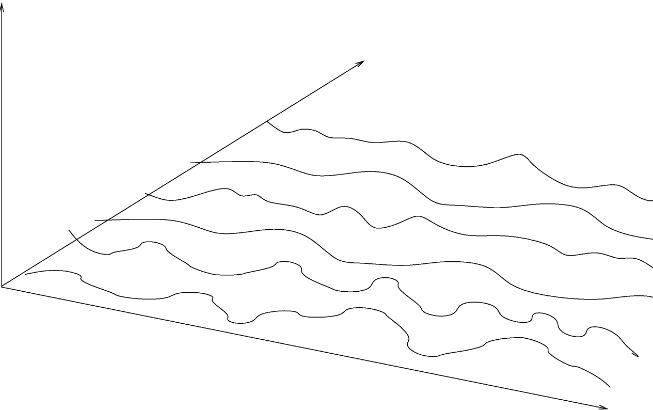
\includegraphics[scale=0.8]{day2_seg1_ranproc1/ensemble.jpg}
\end{frame}

\begin{frame}
  \onslide<1->{
	\frametitle{Random Processes} 
	\framesubtitle{Examples of Discrete Processes: Sampling with Replacement}
}
\begin{itemize}
  \onslide<2->{
			\item A card player shuffles a deck of cards and then picks a card at random.  
}
  \onslide<3->{
			\item He enters the value of the card (1 for an ace through 13 for a king) in an Excel spreadsheet column.  
}
  \onslide<4->{
			\item He then replaces the card and repeats the process over and over again.  
}
  \onslide<5->{
			\item After 10 such experiments, he begins anew with a new Excel column.  Each column represents a new sample trajectory. 
}
\end{itemize}
\end{frame}


\begin{frame}
  \onslide<1->{
	\frametitle{Random Processes} 
	\framesubtitle{Examples of Discrete Processes: MATLAB / Simulink Band-Limited White Noise}
}
\begin{itemize}
  \onslide<2->{
			\item A single source block (band-limited white noise) and a single sink (the scope).
}
  \onslide<3->{
			\item Each time the simulation is run, a new sample trajectory is generated.
}
  \onslide<4->{
			\item Note that this discrete process is created by supposedly sampling a continuous process.    
}
\end{itemize}
\end{frame}


\begin{frame}
  \onslide<1->{
	\frametitle{Random Processes} 
	\framesubtitle{Examples of Discrete Processes: MATLAB / Simulink Band-Limited White Noise}
}
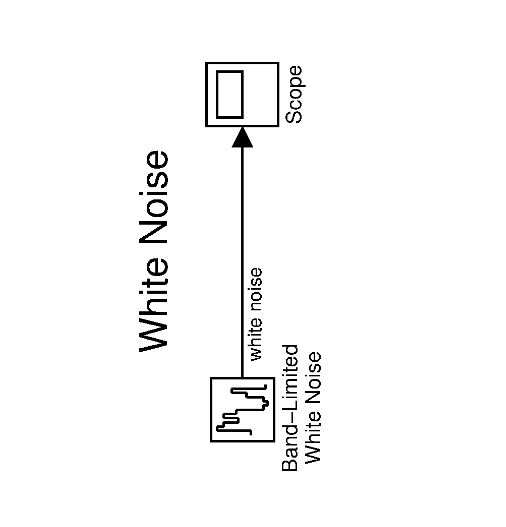
\includegraphics[angle=-90]{day2_seg1_ranproc1/white_noise.jpg}
\end{frame}


\begin{frame}
  \onslide<1->{
	\frametitle{Random Processes} 
	\framesubtitle{Examples:  MATLAB / Simunlink Random Constant}
}
\begin{itemize}
  \onslide<2->{
			\item A single source block (constant block with value generated by random number 
			generator) and a single sink (the scope).
}
  \onslide<3->{
			\item Each time the simulation is run, a new sample trajectory is generated.
}
  \onslide<4->{
			\item Note that this is a continuous process.  
}
\end{itemize}
\end{frame}

\begin{frame}
  \onslide<1->{
	\frametitle{Random Processes} 
	\framesubtitle{Examples:  MATLAB / Simunlink Random Constant}
}
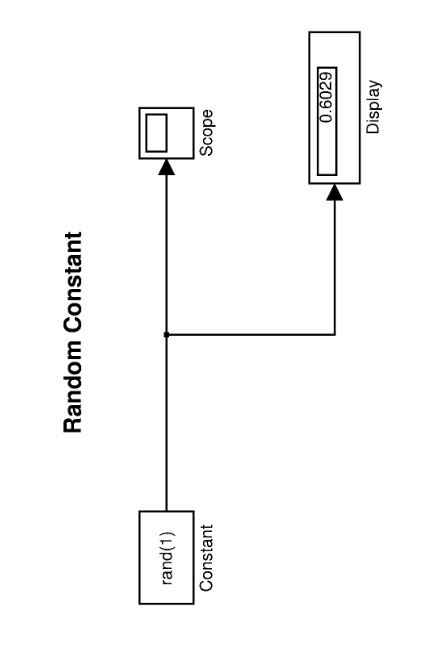
\includegraphics[angle=-90, scale=0.80]{day2_seg1_ranproc1/rand_const1.jpg}
\end{frame}


\begin{frame}
  \onslide<1->{
	\frametitle{Random Processes} 
	\framesubtitle{Examples:  MATLAB / Simunlink Random Constant}
}
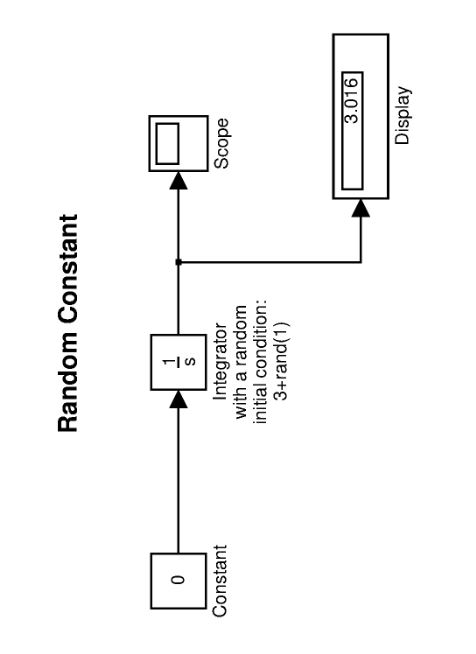
\includegraphics[angle=-90]{day2_seg1_ranproc1/rand_const2.jpg}
\end{frame}

\begin{frame}
  \onslide<1->{
	\frametitle{Random Processes} 
	\framesubtitle{MATLAB / Simulink Sine Wave with Random Phase}
}
\begin{itemize}
  \onslide<2->{
			\item A single source block (sine wave with random phase) and a single sink (the scope)
}
  \onslide<3->{
			\item Each time the simulation is run, a new sample trajectory is generated but 
			each time with a different value for the phase
}
  \onslide<4->{
			\item Note that this is a continuous process  
}
\end{itemize}
\end{frame}


\begin{frame}
  \onslide<1->{
	\frametitle{Random Processes} 
	\framesubtitle{MATLAB / Simulink Sine Wave with Random Phase}
}
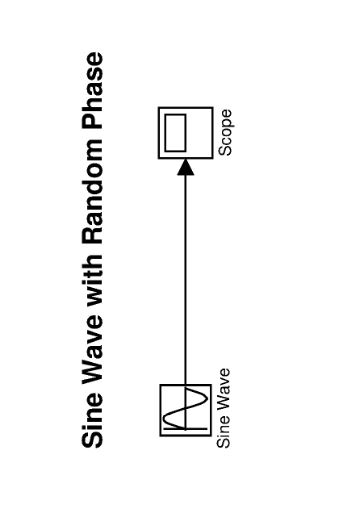
\includegraphics[angle=-90]{day2_seg1_ranproc1/sine_rand_phase.jpg}
\end{frame}

% day2_seg1_ranproc1/stationary.tex
\begin{frame}
  \onslide<1->{
	\frametitle{Random Processes} 
	\framesubtitle{Stationary Random Processes}
}
\begin{itemize}
  \onslide<2->{
 \item A process $X$ is called \textit{\textbf{strongly stationary}} if for
 any finite set of times $\set{t_1,\ldots,t_n}$ and any $\tau>0$
 the two sets of random variables $\set{X(t_1),\ldots,X(t_n)}$ and
$\set{X(t_1+\tau),\ldots,X(t_n+\tau)}$ have identical probability
distributions.
}
  \onslide<3->{
 \item $X$ is called \textit{\textbf{weakly stationary}} if
 \[ \expect{X(s)}=\expect{X(t)}\]
 and
 \[ \expect{X(s)X(t)}=\expect{X(s+\tau)X(t+\tau)}\]
 for all appropriate $\tau>0$ and all times $s,t$.
}
\end{itemize}
\end{frame}

% day2_seg1_ranproc1/corrcov.tex
\begin{frame}
  \onslide<1->{
	\frametitle{Random Processes} 
	\framesubtitle{Correlation and Covariance}
}
\begin{itemize}
  \onslide<2->{
 \item Since at each $t$ $X(t)$ is a random variable in its own right, it makes sense to talk about the correlation of two such random variables $X(t)$ and $X(s)$.
}
  \onslide<3->{
 \item Since both random variables come from the same underlying process, we refer to this as autocorrelation.
}
  \onslide<4->{
 \item Similarly, autocovariance involves first centering the process about its mean process $\mu_t$.
}
\end{itemize}
\end{frame}

\begin{frame}
  \onslide<1->{
	\frametitle{Random Processes} 
	\framesubtitle{Correlation and Covariance}
}
\begin{itemize}
  \onslide<2->{
 \item The function $\expect{X(t)X(t+\tau)}$ is called the \textit{\textbf{autocorrelation
 function}} of $X$ and for a weakly stationary process $X$, and it is denoted by
 $R_{XX}(\tau)$, since it is a function of $\tau$ alone.
}
  \onslide<3->{
 \item The \textit{\textbf{autocovariance}} function for a weakly stationary process is formed
 by subtracting out the means:
 $C_{XX}(\tau)=\expect{(X(t)-\mu_t)(X(t+\tau)-\mu_{t+\tau})}$.
}
  \onslide<4->{
 \item Cross correlation and cross covariance between two different random processes $X$
 and $Y$ are defined in the obvious way.
}
 \onslide<5->{
 \item Note that these are difference than the sample cross correlation and sample cross covariance that 
 we deal with in empirical work
}
\end{itemize}
\end{frame}

\begin{frame}
  \onslide<1->{
	\frametitle{Random Processes} 
	\framesubtitle{Examples of Autocorrelation Functions}
}
\begin{itemize}
  \onslide<2->{
\item Consider the random process $X(t,\omega)=A(\omega)\sin(2\pi f t+\theta)$ in which $A:\Omega\rightarrow \Real$ is a normally distributed random variable with variance $\sigma^2$.
}
  \onslide<3->{
\item The autocorrelation function $R_{XX}(s,t)$ is therefore
\begin{align*}
\expect{X(t,\omega)X(s,\omega)}&=\expect{A(\omega)\sin(2\pi f t+\theta)A(\omega)\sin(2\pi f s+\theta)}\\
&=\expect{A(\omega)^2}\sin(2\pi f t+\theta)\sin(2\pi f s+\theta)\\
&=\sigma^2\sin(2\pi f t+\theta)\sin(2\pi f s+\theta)
\end{align*}
}
\end{itemize}
\end{frame}
\begin{frame}
  \onslide<1->{
	\frametitle{Random Processes} 
	\framesubtitle{Examples of Autocorrelation Functions}
}
\begin{itemize}
  \onslide<2->{
\item Consider the white noise process $W(t)$.
}
  \onslide<3->{
\item Characteristic of white noise to be uncorrelated in time
}
  \onslide<4->{
\item Thus, $\expect{W(t)W(s}=0$ for every $s$ and $t$ such that $s\neq t$.
}
\end{itemize}
\end{frame}

\begin{frame}
  \onslide<1->{
	\frametitle{Random Processes} 
	\framesubtitle{Ergodic Processes}
}
\begin{itemize}
  \onslide<2->{
 \item We shall be concerned almost exclusively with weakly
 stationary processes that are also \textbf{ergodic}, meaning that ensemble
 averaging at any one time gives the same result as time averaging
 one sample trajectory.  Thus we may assume:
}
  \onslide<3->{
\begin{equation}\label{ergodic_mean}
  \mu_X=\limint X(t)dt
\end{equation}
}
  \onslide<4->{
\begin{equation}\label{ergodic_meansquare}
  \psi_X^2 = \limint X^2(t)dt
\end{equation}
}
  \onslide<5->{
\begin{equation}\label{ergodic_autocorr}
  R_{XX}(\tau)=\limint X(t)X(t+\tau)dt
\end{equation}
}
\end{itemize}
\end{frame}

\begin{frame}
  \onslide<1->{
	\frametitle{Random Processes} 
	\framesubtitle{Ergodic Processes}
}
\begin{itemize}
  \onslide<2->{
 \item We haven't yet defined want we mean by such time integrals,
 however, so we have to hold off dealing with them.
}
  \onslide<3->{
 \item Once we have defined the mean square limit of
 Riemann-Stieltjes sums, then we'll know what these integrals
 really mean.
}
  \onslide<4->{
 \item Nevertheless, if we fix $\omega$ and consider only sample trajectories $X(t,\omega)$, then we can use ordinary integrals provided that the sample trajectories are well-enough behaved.
}
\end{itemize}
\end{frame}

\begin{frame}
  \onslide<1->{
	\frametitle{Random Processes} 
	\framesubtitle{Ergodic Processes}
}
\begin{itemize}
  \onslide<2->{
 \item Well-behaved means that they are of bounded variation, i.e., they don't wiggle around too much.
}
  \onslide<3->{
 \item Unfortunately, this doesn't really work for the usual conception of white noise, because its sample trajectories are not of bounded variation.
}
  \onslide<4->{
 \item If we restrict our attention to band-limited white noise (like Matlab / Simulink does), then we can stick to the ordinary integrals we learned in calculus.
}
\end{itemize}
\end{frame}

% day2_seg1_ranproc1/psd.tex
\begin{frame}
  \onslide<1->{
	\frametitle{Random Processes} 
	\framesubtitle{Power Spectral Density}
}
\begin{itemize}
  \onslide<2->{
 \item The \textit{\textbf{power spectral density}} (PSD) function is the
 Fourier transform of the autocorrelation function:
\begin{equation}\label{psd}
  P_{XX}(\omega)=\infint R_{XX}(\tau)\exp(-j\omega\tau)d\tau
\end{equation}
where $j=\sqrt{-1}$ and $\omega$ is angular frequency in rad/sec (not an outcome of the sample space!).
}
  \onslide<3->{
 \item Units:  If $X$ is in volts(V), then
 $P_{XX}$ has units of $\text{V}^2/(2\pi \text{Hz})$ or $\text{V}^2\;\text{sec}/\text{rad}$, 
 due to $R_{XX}$ being a product of samples in volts and transform kernel
 being in 1/rad:
 $\exp(-j\omega\tau)=\frac{1}{\exp(j\omega\tau)}$.  $d\tau$ is in sec.
}
 \onslide<4->{
	\item Note: $2\pi\text{ rad/cycle }1\text{Hz}=2\pi\text{ rad/cycle }1\text{ cycle}/\text{sec}=2\pi\text{ rad/sec}$.
 }
\end{itemize}
\end{frame}
\begin{frame}
  \onslide<1->{
	\frametitle{Random Processes} 
	\framesubtitle{Power Spectral Density}
}
\begin{itemize}
  \onslide<2->{
 \item Sometimes the definition in equation \eqref{psd} is referred to as the autospectral
 density, since the autocorrelation function is involved
}
  \onslide<3->{
 \item The cross-spectral density function is defined in the same
 way, but with $R_{XY}$ substituted for $R_{XX}$
}
\end{itemize}
\end{frame}

\begin{frame}
  \onslide<1->{
	\frametitle{Random Processes} 
	\framesubtitle{Power Spectral Density}
}
\begin{itemize}
  \onslide<2->{
\item Another way to obtain power spectral density is through
 Fourier transform of the original process
}
 \onslide<3->{
\item Let's change our notation:  We've been using uppercase letters such as $X$ and $Y$ to
denote random variables and processes and we've been using $\omega$ to denote a
point of the sample space $\Omega$
}
  \onslide<4->{
\item Now we'll use lowercase letters like $x(t)$ and $y(t)$
to denote processes in the time domain but uppercase letters for
Fourier transforms in the frequency domain  
}
  \onslide<5->{
\item Also, lowercase $\omega$ will often stand for frequency in rad/sec
}
\end{itemize}
\end{frame}
\begin{frame}
  \onslide<1->{
	\frametitle{Random Processes} 
	\framesubtitle{Power Spectral Density}
}
\begin{itemize}
  \onslide<2->{
\item The finite Fourier transform of a random process $x(t)$ is
\[X(\omega,T)=\int_0^Tx(\tau)\exp(-j\omega\tau)d\tau\]
}
  \onslide<3->{
\item The PSD can be expressed as follows:
\begin{equation}\label{wiener_khinchin}
  P_{XY}(\omega) = \lim_{T\rightarrow \infty}\frac{1}{T}\expect{X^*(\omega,T)Y(\omega,T)}
\end{equation}
where $X(\omega,T)$ and $Y(\omega,T)$ are the finite Fourier
transforms of $x(t)$ and $y(t)$, respectively, and
$X^*(\omega,t)$ is the complex conjugate of $X(\omega,t)$. \\
$\omega$ is frequency in rad/sec.
}
  \onslide<4->{
\item Both Eq. \eqref{wiener_khinchin} and \eqref{psd} are referred to as the Wiener-Khinchin equation
}
\end{itemize}
\end{frame}


%% day2_seg1_ranproc1/exercises.tex
\begin{frame}
Exercises
 \begin{itemize}
 \item
 \item
 \item
\end{itemize}
\end{frame}


% day2_seg2_ranproc2/ranproc2_main.tex
\begin{frame}
  \onslide<1->{
	\frametitle{Random Processes} 
	\framesubtitle{Some Important Random Processes}
}
\begin{itemize}
  \onslide<2->{
 \item White Noise
}
  \onslide<3->{
 \item Random Walk
}
  \onslide<4->{
 \item Random Constant
}
  \onslide<5->{
 \item Random Ramp
}
  \onslide<6->{
 \item Second Order Processes:  Gaussian, and Gauss-Markov Processes
}
  \onslide<7->{
 \item State Space Augmentation
}
\end{itemize}
\end{frame}

% day2_seg2_ranproc2/white_noise.tex
\begin{frame}
  \onslide<1->{
	\frametitle{Some Important Random Processes} 
	\framesubtitle{White Noise}
}
\begin{itemize}
  \onslide<2->{
 \item White noise can be defined as a process whose
 autocorrelation function is a Dirac delta function:
\begin{equation}\label{dirac}
  \delta(\tau)=
  \begin{cases}
    \infty & \text{if }, \tau=0 \\
    0 & \text{otherwise}.
  \end{cases}
\end{equation}
}
  \onslide<3->{
 \item There's only one mathematical problem:  this is not a real function
}
  \onslide<4->{
 \item There's also a physical problem:  such a process would have
 infinite mean-squared value and hence infinite energy
}
\end{itemize}
\end{frame}
\begin{frame}
  \onslide<1->{
	\frametitle{Some Important Random Processes} 
	\framesubtitle{White Noise}
}
\begin{itemize}
  \onslide<2->{
 \item There is a way to properly define the Dirac delta as a linear functional (a distribution) rather than 
 a function, and to show that it retains all of its desired properties
  }
  \onslide<3->{
 \item However, we'll proceed as if this concept of white noise were well-defined and use the 
 delta function's integration properties to define some other processes such as random walk.
}
  \onslide<4->{
 \item Characteristic feature of white noise to be uncorrelated in time.  This is the intent of using the 
 Dirac delta functional as its defining autocorrelation function
}
\end{itemize}
\end{frame}
\begin{frame}
  \onslide<1->{
	\frametitle{Some Important Random Processes} 
	\framesubtitle{White Noise}
}
\begin{itemize}
  \onslide<2->{
 \item MATLAB / Simulink block for white noise makes it a bandlimited signal, so that the bandwidth is not 
 infinite as it otherwise would be for pure white noise
}
  \onslide<3->{
 \item Valid assumption as long as noise bandwidth is
 sufficiently greater than that of the system under consideration
 }
  \onslide<4->{
 \item In MATLAB you can simulate a discrete white noise sequence
 by drawing a random number at each time step from a normal distribution
}
  \onslide<5->{
 \item Bottom line:  Random sequence for white noise needs to have a correlation time much smaller than 
 the shortest time constant of the system
}
\end{itemize}
\end{frame}


% day2_seg2_ranproc2/rand_walk.tex
\begin{frame}
  \onslide<1->{
	\frametitle{Some Important Random Processes} 
	\framesubtitle{Random Walk}
}
\begin{itemize}
  \onslide<2->{
 \item In engineering applications, random walk is often considered as a discrete time process.
}
  \onslide<3->{
 \item Some authors (Gelb, for example) refer to continuous-time random walk as the
 solution of a differential equation driven by white noise:
 $\dot{x}=w$.
}
  \onslide<4->{
 \item However, that would require $w$ to be integrable which it is not, because it is not of bounded variation.  
 Alternatively, it would require the Wiener-Levy process to be differentiable, which it is not
}
  \onslide<5->{
 \item So we'll stick to the bandlimited or the discrete case: $x(k+1)=x(k) + w(k)$,
 where the $w(k)$ are normally distributed and statistically uncorrelated at distinct sample times
}
\end{itemize}
\end{frame}

\begin{frame}
  \onslide<1->{
	\frametitle{Some Important Random Processes} 
	\framesubtitle{Random Walk:  Bandlimited White Noise is Integrable}
}
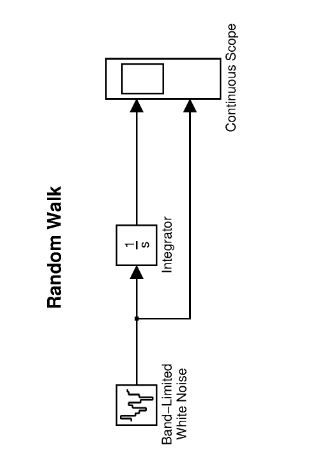
\includegraphics[angle=-90, scale=0.80]{day2_seg2_ranproc2/rand_walk.jpg}
\end{frame}

\begin{frame}
  \onslide<1->{
	\frametitle{Some Important Random Processes} 
	\framesubtitle{Discrete Random Walk}
}
\begin{itemize}
  \onslide<2->{
\item  $x(k)=x(k-1)+w(k)$, where $w(k)$ is a white sequence 
}
  \onslide<3->{
\item  Another way of looking at this is to say that the difference sequence is white:  $x(k)-x(k-1)=w(k)$ 
}
  \onslide<4->{
\item  In MATLAB you can use the diff function to create the difference sequence from a give sequence. Note that 
it would have 1 less element than the original sequence:\\
x=rand(1,5); dx=diff(x);\\
x =    [ 1,     0,     2,    -1,     4]\\
dx =  [-1,     2,    -3,     5] 
}
\end{itemize}
\end{frame}

\begin{frame}
  \onslide<1->{
	\frametitle{Some Important Random Processes} 
	\framesubtitle{Discrete Random Walk:  Raytheon Stock Price (4000 daily samples)}
}
\begin{center}
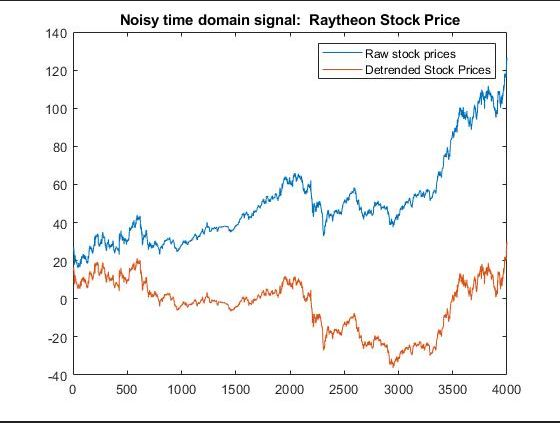
\includegraphics[scale=0.50]{day2_seg2_ranproc2/rtn_stock_prices.jpg}
\end{center}
\end{frame}
 
\begin{frame}
  \onslide<1->{
	\frametitle{Some Important Random Processes} 
	\framesubtitle{Discrete Random Walk:  Raytheon Stock Price Power Spectal Density}
}
\begin{center}
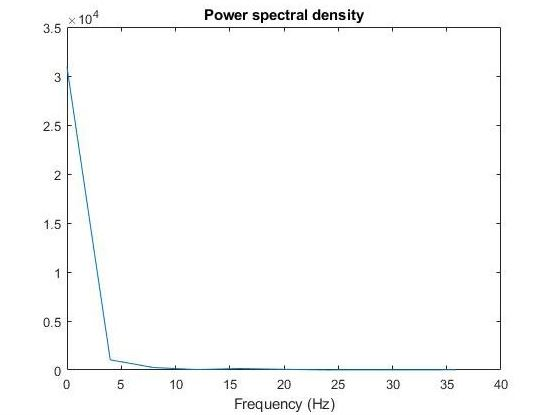
\includegraphics[scale=0.50]{day2_seg2_ranproc2/rtn_randwalk.jpg}
\end{center}
\end{frame}

\begin{frame}
  \onslide<1->{
	\frametitle{Some Important Random Processes} 
	\framesubtitle{Discrete Random Walk:  Detrened Difference of Raytheon Stock Price}
}
Let's see if the difference sequence of detrended stock prices looks like white noise:
\begin{center}
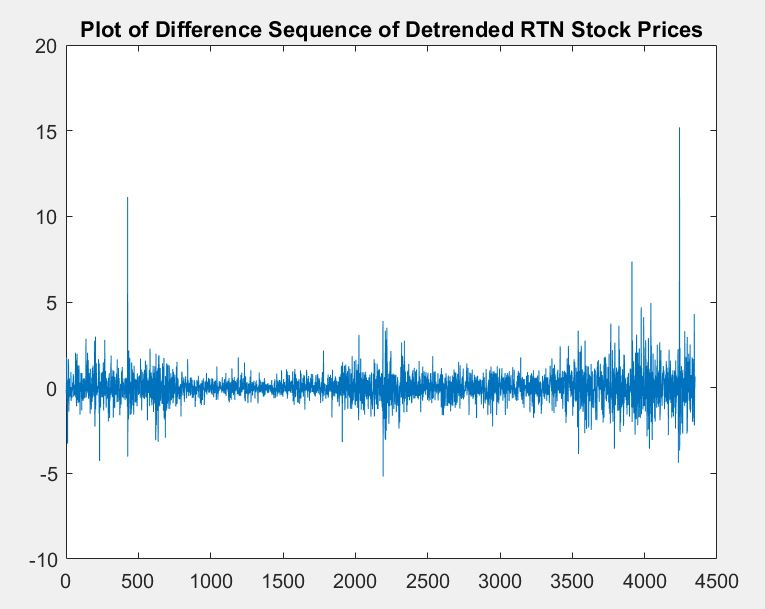
\includegraphics[scale=0.50]{day2_seg2_ranproc2/rtn_stock_prices_diff_detrended.jpg}
\end{center}
\end{frame}

% day2_seg2_ranproc2/rand_ramp.tex
\begin{frame}
  \onslide<1->{
	\frametitle{Some Important Random Processes} 
	\framesubtitle{Random Constant and Random Ramp}
}
\begin{itemize}
  \onslide<2->{
 \item A random constant process $x$ such that the sample trajectories are constant with respect to time\\
\begin{footnotesize} But the constant value is different for each sample trajectory in the ensemble\\
$x(\omega_1,t)\neq x(\omega_2,t)$, for $\omega_1\neq \omega_2$
\end{footnotesize}
}
  \onslide<3->{
 \item A random ramp requires two state variables: a random constant (y-intercept or bias) and the integral of a
 random constant (yields random slope)
}
  \onslide<4->{
 \item In principle,
 however, this constant value could vary with $\omega$, i.e., across the
 ensemble, thus making the process non-Ergodic.
}
  \onslide<5->{
 \item Random constants are very useful in many applications to model biases that vary from
 turn-on to turn-on
}
\end{itemize}
\end{frame}
\begin{frame}
  \onslide<1->{
	\frametitle{Some Important Random Processes} 
	\framesubtitle{Random Constant and Random Ramp}
}
\begin{itemize}
  \onslide<2->{
 \item See Matlab Simulink demos:  rand\_const.mdl and
 rand\_ramp.mdl
}
  \onslide<3->{
 \item In modeling gyro biases, a combination of a random constant
 (bias stability) and random walk (bias drift) is common.
}
  \onslide<4->{
 \item Gyro scale factors are modeled similarly.
}
  \onslide<5->{
 \item Deterministic biases and scale factors are also part of the model, but these generally are calibrated out.
}
\end{itemize}
\end{frame}

% day2_seg2_ranproc2/markov_proc.tex
\begin{frame}
  \onslide<1->{
	\frametitle{Some Important Random Processes} 
	\framesubtitle{Second Order Processes}
}
\begin{itemize}
  \onslide<2->{
 \item We will generally restrict our attention to \textit{\textbf{second-order processes}}, i.e., those such that
 $X(t)\in L^2(\Omega)$.
 \item Recall what this means:
 \[\expect{X^2(t)}<\infty\]
}
  \onslide<3->{
 \item This allows us to use Hilbert space techniques because, for
 every $s,t\in[0,T]$, $\expect{X(s)Y(t)}$ is an inner
 product.  Inner products, norms and metrics allow us to do
 calculus and geometry (orthogonal projection).
}
\end{itemize}
\end{frame}

\begin{frame}
  \onslide<1->{
	\frametitle{Some Important Random Processes} 
	\framesubtitle{Orthogonal Projection}
}
\begin{center}
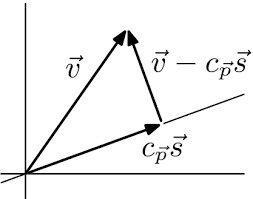
\includegraphics[scale=0.6]{graphics/orthoproj.png}
\end{center}
\end{frame}


\begin{frame}
  \onslide<1->{
	\frametitle{Some Important Random Processes} 
	\framesubtitle{Gaussian Processes}
}
\begin{itemize}
  \onslide<2->{
 \item An important class of second-order processes are the
 Gaussian processes.
}
  \onslide<3->{
\item Let $X:[0,T]\rightarrow L^2(\Omega)$ be a second-order
 process.  $X$ is said to be \textit{\textbf{Gaussian}} if for every finite set of times $\set{t_1,\ldots,t_n}$
 the vector of random variables $(X(t_1),\ldots,X(t_n))$ has a
 multivariate normal distribution.
}
  \onslide<4->{
  \item To fully appreciate what this means, we need to explain
 what a multivariate normal distribution is.
}
\end{itemize}
\end{frame}

\begin{frame}
  \onslide<1->{
	\frametitle{Some Important Random Processes} 
	\framesubtitle{Gaussian Processes}
}
\begin{itemize}
  \onslide<2->{
 \item A function $Q_C:\Real^n\rightarrow \Real$ of the form
 \[Q_C(x)=x\trans C x\]
 where $x\in\Real^n$ is a column vector and $C$ is a real symmetric
 matrix., is called a \textit{\textbf{quadratic form}} associated with $C$. (I.e., $C=(c_{ij})$ and $c_{ij}=c_{ji}$).
}
  \onslide<3->{
 \item We will further assume that $C$ is positive definite, which
 means that $Q_{C}(x)>0$ for every non-zero vector $x$.
}
\end{itemize}
\end{frame}

\begin{frame}
  \onslide<1->{
	\frametitle{Some Important Random Processes} 
	\framesubtitle{Gaussian Processes}
}
\begin{itemize}
  \onslide<2->{
 \item Then $X_1,\ldots,X_n$ are said to have a \textit{\textbf{multivariate normal distribution}}
 if their joint p.d.f. is of the form
\begin{equation}\label{gaussvec}
  f(x_1,\ldots,x_n)=\gvpdf
\end{equation}
for a real, positive definite symmetric matrix $C$ and
$\mu=(\mu_1,\ldots,\mu_n)$.
}
  \onslide<3->{
 \item $C$ is called the \textit{\textbf{covariance matrix}} and $\mu$ is called the
 \textit{\textbf{mean}} vector.
}
\end{itemize}
\end{frame}

\begin{frame}
  \onslide<1->{
	\frametitle{Some Important Random Processes} 
	\framesubtitle{Gaussian Processes}
}
\begin{itemize}
  \onslide<2->{
 \item In terms of quadratic forms, this is
 \[f(x_1,\ldots,x_n)= \sqrt{\frac{\det(C^{-1})}{(2\pi)^n }}
  \exp\left[ -\frac{1}{2}Q_{C^{-1}}(x-\mu) \right]\]
}
  \onslide<3->{
\item $C^{-1}$ is sometimes called the information matrix,
 because its inverse, the covariance matrix, often expresses the
 uncertainty (or lack of information) associated with the random
 variables.
}
\end{itemize}
\end{frame}

\begin{frame}
  \onslide<1->{
	\frametitle{Some Important Random Processes} 
	\framesubtitle{Gaussian Processes}
}
\begin{itemize}
  \onslide<2->{
\item Thus a Gaussian process is a random process for which the
 joint distribution of every finite collection of range random
 variables is a Gaussian distribution.
}
  \onslide<3->{
  \item The Gaussian process is important in connection with the
 kinds of noise that drive the dynamic systems we are interested
 in.
}
  \onslide<4->{
 \item The linear Kalman filter is optimal only under assumptions
 that the process noise and the measurement noise are Gaussian.
}
\end{itemize}
\end{frame}

\begin{frame}
  \onslide<1->{
	\frametitle{Some Important Random Processes} 
	\framesubtitle{Gauss-Markov Processes}
}
\begin{itemize}
  \onslide<2->{
 \item A Gauss-Markov process is for which the autocorrelation
 function has an exponential form:
\begin{equation}\label{gauss-markov}
  R_{XX}(\tau) = \sigma^2\exp(-\beta\abs{\tau})
\end{equation}
}
  \onslide<3->{
\item As a continuous-time dynamic system, this would correspond to passing white
 noise through first-order feedback system:
 \[\dot{x}=-\beta x+w\]
 \item See Matlab Simulink file gauss\_markov.mdl
}
\end{itemize}
\end{frame}

\begin{frame}
  \onslide<1->{
	\frametitle{Some Important Random Processes} 
	\framesubtitle{Gauss-Markov Processes}
}
\begin{itemize}
  \onslide<2->{
\item Discrete version of a Gauss-Markov process:
\[
x(k+1)=\exp\left(-\beta \Delta t\right)x(k) + w(k)
\]
where $\Delta t = t_{k+1}-t_k$ and is assumed to be the same regardless of $k$, and $w(k)$ is a white noise sequence
}
\end{itemize}
\end{frame}
\begin{frame}
  \onslide<1->{
	\frametitle{Some Important Random Processes} 
	\framesubtitle{Gauss-Markov Processes:  Simulink Model}
}
\begin{center}
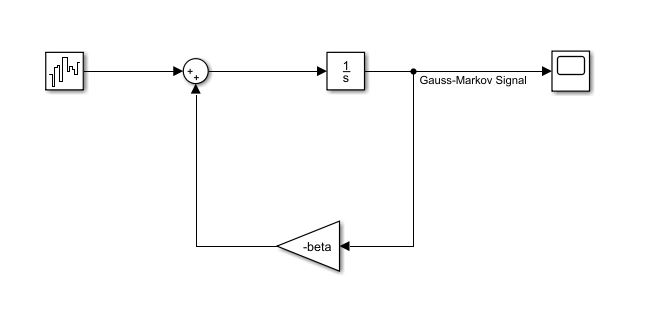
\includegraphics[scale=0.60]{day2_seg2_ranproc2/gauss_markov.jpg}
\end{center}
\end{frame}
\begin{frame}
  \onslide<1->{
	\frametitle{Some Important Random Processes} 
	\framesubtitle{Gauss-Markov Processes:  Output of Simulink Model}
}
\begin{center}
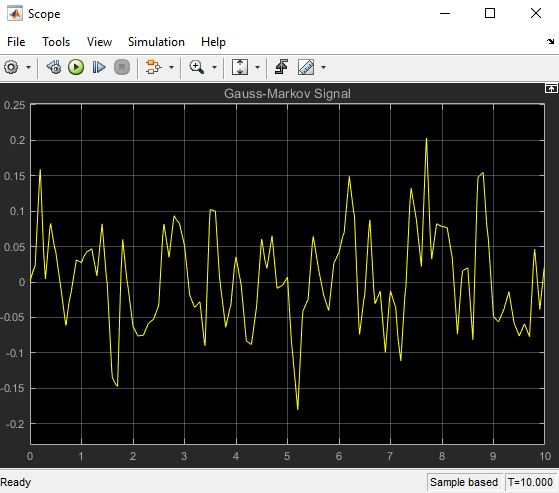
\includegraphics[scale=0.50]{day2_seg2_ranproc2/gauss_markov_scope.jpg}
\end{center}
\end{frame}

% day2_seg2_ranproc2/state_space_aug.tex
\begin{frame}
  \onslide<1->{
	\frametitle{State Space Augmentation} 
	\framesubtitle{Motivation}
}
\begin{itemize}
  \onslide<2->{
 \item Kalman filter theory assumes the only remaining forcing function is white process noise
}
  \onslide<3->{
 \item The most frequently used models can all be understood as differential equations (or difference equations) 
 driven by white noise
}
  \onslide<4->{
 \item If assumption of the only forcing function being white is not satisfied due to presence of colored noise, 
 then the colored noise can be whitened
}
  \onslide<5->{
 \item Otherwise, new states need to be added:  this is called state vector or state space \textbf{augmentation}
}
  \onslide<6->{
 \item We'll see an example of state space augmentation later when we discuss filter maintenance
}
\end{itemize}
\end{frame}

\begin{frame}
  \onslide<1->{
	\frametitle{State Space Augmentation} 
	\framesubtitle{General Example:  Augmenting a 2-State Model}
}
\begin{itemize}
  \onslide<2->{
\item Given 2-state model:  
\[
\begin{bmatrix}
\dot{x}_1\\
\dot{x}_2

\end{bmatrix} =
\begin{bmatrix}
a_{11} & a_{12}\\
a_{21} & a_{22}
\end{bmatrix}
\begin{bmatrix}
x_1\\
x_2
\end{bmatrix}+
\begin{bmatrix}
w_1\\
w_2
\end{bmatrix}
\]  
}
  \onslide<3->{
\item  Suppose the "noise" is not actually white;  perhaps there is some long-term drift as exhibited by random walk
}
  \onslide<4->{
\item   This means that $\dot{w}_i=\epsilon_i$, where $\epsilon_i$ is white
}
  \onslide<5->{
\item We augment with new states $x_3=w_1,x_4=w_2$ as follows: 
\[
\begin{bmatrix}
\dot{x}_1\\
\dot{x}_2\\
\dot{x}_3\\
\dot{x}_4

\end{bmatrix} =
\begin{bmatrix}
a_{11} & a_{12} & 1 & 0\\
a_{21} & a_{22} & 0 & 1\\
0 & 0 & 0 & 0\\
0 & 0 & 0 & 0
\end{bmatrix}
\begin{bmatrix}
x_1\\
x_2\\
x_3\\
x_4
\end{bmatrix}+
\begin{bmatrix}
0 & 0 & 0 & 0\\
0 & 0 & 0 & 0\\
0 & 0 & 1 & 0\\
0 & 0 & 0 & 1

\end{bmatrix}
\begin{bmatrix}
0\\
0\\
\epsilon_1\\
\epsilon_2
\end{bmatrix}
\]  
}
\end{itemize}
\end{frame}
\begin{frame}
  \onslide<1->{
	\frametitle{State Space Augmentation} 
	\framesubtitle{}
}
\begin{itemize}
  \onslide<2->{
\item   If original measurement was, say,
\[
\begin{bmatrix}
z_1\\
z_2
\end{bmatrix}=
\begin{bmatrix}
1 & 0\\
0 & 1
\end{bmatrix}
\begin{bmatrix}
x_1\\
x_2
\end{bmatrix}+
\begin{bmatrix}
v_1\\
v_2
\end{bmatrix}
\]
}
  \onslide<3->{
\item  It now becomes, after augmentation: 
\[
\begin{bmatrix}
z_1\\
z_2
\end{bmatrix}=
\begin{bmatrix}
1 & 0 & 0 & 0\\
0 & 1 & 0 & 0
\end{bmatrix}
\begin{bmatrix}
x_1\\
x_2\\
x_3\\
x_4
\end{bmatrix}+
\begin{bmatrix}
v_1\\
v_2
\end{bmatrix}
\]
}
\end{itemize}
\end{frame}
\begin{frame}
  \onslide<1->{
	\frametitle{State Space Augmentation} 
	\framesubtitle{How can you tell when to augment your state vector?}
}
\begin{itemize}
  \onslide<2->{
\item To determine if state vector augmentation is needed, look at the pre-fit residual sequence:  $\nu(k)=\innovation{k}$  
}
  \onslide<3->{
\item Examine its autocorelation function $R_{\nu\nu}$ (or autospectal density)  
}
  \onslide<4->{
\item Determine the correlation time constant and augment the state vector with a Gauss-Markov process with the appropriate
time constant in the feedback gain 
}
  \onslide<5->{
\item Alternatively, you can examine the autospectal density graph and eyeball a correlation constant (See Grewal handouts.)  
}
\end{itemize}
\end{frame}


% day2_seg2_ranproc2/exercises.tex
\begin{frame}
  \onslide<1->{
	\frametitle{Exercises} 
}
  \onslide<2->{
 1. Perform the following random walk experiment: \\
a. Create a graph with two axes marked off at integral (discrete) points.\\
b. Plot the first point at the origin.\\
c. Flip a coin.  If the result is heads, move one step to the right and plot a point 1 unit above the previous y value.  If the result is tails, move one step to the right and plot a point 1 unit below the previous y value.\\
d. Repeat step c ten times.\\
}
  \onslide<3->{
2.  What is your estimate for how the variance of this process grows with time?\\
}
  \onslide<4->{
3. As a class exercise, we'll compute the ensemble averages across the class results at each point.  Is this pocess ergodic?
}
\end{frame}


% day2_seg3_kalstats/kalstats_main.tex
\begin{frame}
  \onslide<1->{
	\frametitle{Kalman Statistics}
		\framesubtitle{Topics}
}
\begin{itemize}
  \onslide<2->{
 \item Covariance Matrices
}
  \onslide<3->{
 \item Process Noise Covariance Matrix $Q$
}
  \onslide<4->{
 \item Measurement Noise Covariance Matrix $R$
}
 \onslide<5->{
  \item Estimation Error Covariance Matrix $P$
 }
 \onslide<6->{
  \item Kalman Assumptions
 }
  \onslide<7->{
 \item The Static Estimation Problem:  Bayesian Derivation of the Kalman Gain
}
\end{itemize}
\end{frame}
% day2_seg3_kalstats/cov_mat.tex
\begin{frame}
  \onslide<1->{
	\frametitle{Covariance Matrices} 
	\framesubtitle{$Q,R,P$}
}
\begin{itemize}
  \onslide<2->{
 \item There are several covariance matrices associated with the Kalman filter: 
 $ \procnoisemat{k},\measnoisemat{k}, P(k)$
}
  \onslide<3->{
 \item In general, a covariance matrix is associated with a random vector $X$ as in the following definition:
\[C_X = \expect{XX\trans}\]
}
\end{itemize}
\end{frame}
\begin{frame}
  \onslide<1->{
	\frametitle{Covariance Matrices} 
	\framesubtitle{$Q,R,P$}
}
\begin{itemize}
  \onslide<2->{
 \item This is precisely how $\procnoisemat{k}$ and $\measnoisemat{k}$ are defined:
\[\procnoisemat{k}=\expect{w(k)w\trans(k)}\] and
\[\measnoisemat{k}=\expect{v(k)v\trans(k)}\]
}
  \onslide<3->{
\item $\covmat{k}{+}$, on the other hand is called the error covariance, because it is associated with $\esterr$
\[\covmatdef\]
where $\esterrdef$.
}
\end{itemize}
\end{frame}
\begin{frame}
  \onslide<1->{
	\frametitle{Covariance Matrices} 
	\framesubtitle{Positive Definite Symmetric Matrices}
}
\begin{itemize}
  \onslide<2->{
\item Covariance Matrices are \textbf{positive definite}: The quadratic form $x\trans C x>0$ for all nonzero vectors $x$  
}
  \onslide<3->{
\item We write $C>0$ for positive definite matrices  
}
  \onslide<4->{
\item $C>0$ iff all eigenvalues of $C$ are positive 
}
  \onslide<5->{
\item All diagonal elements of $C$ are positive if $C>0$  
}
  \onslide<6->{
\item If $C>0$ and $S$ non-singular (invertible), then $SCS\trans>0$ and $S\trans CS>0$
}
  \onslide<7->{
\item If $C>0$ then $C$ is non-singular and $C^{-1}>0$
}
\end{itemize}
\end{frame}

\begin{frame}
  \onslide<1->{
	\frametitle{Covariance Matrices} 
	\framesubtitle{Lower Triangular Cholesky Decomposition}
}
\begin{itemize}
  \onslide<2->{
\item  If $C>0$ then a lower triangular matrix $L$ can be found such that $C=LL\trans$ 
}
  \onslide<3->{
\item $L$ is called a \textbf{matrix square root} of $C$  
}
  \onslide<4->{
\item  Square root matrices are not unique;  $TL$ is also a square root of $C$ if $L$ is such and if $T$ is orthogonal $TT\trans=I$ 
}
  \onslide<5->{
\item We'll learn more about square root matrices when we study square root filtering  
}
\end{itemize}
\end{frame}

% day2_seg3_kalstats/proc_noise.tex
\begin{frame}
  \onslide<1->{
	\frametitle{Process Noise} 
	\framesubtitle{Characteristics}
}
\begin{itemize}
  \onslide<2->{
 \item The process noise $w(k)$ is assumed to be a white, zero-mean, Gaussian sequence.
}
  \onslide<3->{
 \item Although the continuous-time form of white noise does not really exist, it is sufficient in the 
 discrete-time case  to consider a random process sequence $w(k)$ that is uncorrelated from 
 step to step: $\expect{w(j)w\trans (k)}=0$ 
 if $j\neq k$
}
  \onslide<4->{
 \item This can be achieved if $w(k)$ is the result of sampling a Gauss-Markov process whose exponential 
autocorrelation function rapidly approaches 0 before the next sample is taken 
}
  \onslide<5->{
\item  Process noise is is thought to arise from unmodelled or negligible states that in aggregate 
behave is a normally-distributed fashion 
}
\end{itemize}
\end{frame}


\begin{frame}
  \onslide<1->{
	\frametitle{Process Noise} 
	\framesubtitle{Process Noise Covariance Matrix $Q$}
}
\begin{itemize}
  \onslide<2->{
\item Process noise covariance matrix $Q$ affects the Kalman gain indirectly through the 
covariance propagation equation for $\covmat{k}{-}$:
\[\altcovextrapeq\]
}
  \onslide<3->{
\item This updated error covariance is then included in both the "numerator" and "denominator" of the Kalman gain:
\[\kalgaineq\]
}
  \onslide<4->{
\item If $Q$ is large relative to $R$ then $K\approx I$ causing $\hat{x}^{-}$ to cancel out and 
the updated state estimate $\hat{x}^{+}$ will be nearly identical to the measurement $z$
}
\end{itemize}
\end{frame}

\begin{frame}
  \onslide<1->{
	\frametitle{Process Noise} 
	\framesubtitle{Importance for Filter Tuning}
}
\begin{itemize}
  \onslide<2->{
\item Since $w(k)$ is an unknown, random forcing function, its parameters have to be selected in a 
process called \textbf{filter tuning}  
}
  \onslide<3->{
\item  Filter tuning means selecting appropriate values for the entries of $Q$ 
}
  \onslide<4->{
\item Techniques to augment the state vector are also used to tune the process noise
}
  \onslide<5->{
\item  Process noise covariance $Q$ is one of two key tuning parameters, the other being measurement noise covariance $R$
}
\end{itemize}
\end{frame}


% day2_seg3_kalstats/meas_noise.tex
\begin{frame}
  \onslide<1->{
	\frametitle{Measurement Noise} 
	\framesubtitle{$v$ and its Covariance Matrix $R$}
}
\begin{itemize}
  \onslide<2->{
\item  $\measnoise{k}$ is the measurement noise sequence;  unlike $w(k)$ it is not simply hypothesized; 
it is physically real and  can be determined empirically
}
  \onslide<3->{
 \item The measurement noise covariance matrix $\measnoisematdef{k}$ indicates the amount of spread or dispersion and internal cross covariance within the measurement itself at any time $k$.
}
  \onslide<4->{
 \item The diagonal elements of $\measnoise{k}$ give the expected variance in each of the individual measurements.
}
\end{itemize}
\end{frame}

\begin{frame}
  \onslide<1->{
	\frametitle{Measurement Noise} 
	\framesubtitle{Characteristics of $R$}
}
\begin{itemize}
  \onslide<2->{
 \item The off-diagonal elements indicate degree of cross covariance between measurement noise random variables 
 associated with each individual measurement;  often 0  
}
  \onslide<3->{
 \item If the noise random variables of individual measurements are uncorrelated, 
 then $R(k)$ will be a diagonal matrix
}
  \onslide<4->{
\item General time series and spectral analysis techniques can be applied to a sequence measurements to determine appropriate values
}
  \onslide<5->{
\item The elements of $R$ are key Kalman tuning parameters
}
\end{itemize}
\end{frame}

\begin{frame}
  \onslide<1->{
	\frametitle{Comparison of Process Noise and Measurement Noise} 
	\framesubtitle{$Q$ vs $R$}
}
\begin{itemize}
  \onslide<2->{
\item If $Q$ is large relative to $R$, then $K\approx I$, the extrapolated state estimate will cancel out in the state update 
equation; the updated state estimate will consist essentially only of the measurement $z$
}
  \onslide<3->{
\item This can be seen as follows in the special case that $H(k)$ is square and invertible:
\begin{footnotesize}
\begin{align*}
\stateest{k}{+}&=\stateest{k}{-}+\kalgain{k}\left[\innovation{k}\right]\\
&\approx \stateest{k}{-}+\covmat{k}{-}H(k)\trans\left[H(k)\covmat{k}{-}H(k)\trans\right]^{-1}\left[\innovation{k}\right]\\
&= \stateest{k}{-}+\\
&\;\;\;\;\;\;\;\;\covmat{k}{-}H(k)\trans
\left[H(k)\trans\right]^{-1}\left[\covmat{k}{-}\right]^{-1}H(k)^{-1}\left[\innovation{k}\right]\\
&= \stateest{k}{-}+H(k)^{-1}z(k)-\stateest{k}{-}\\
&= H(k)^{-1}z(k)
\end{align*}
\end{footnotesize}
}
\end{itemize}
\end{frame}


\begin{frame}
  \onslide<1->{
	\frametitle{Comparison of Process Noise and Measurement Noise} 
	\framesubtitle{$Q$ vs $R$}
}
\begin{itemize}
  \onslide<2->{
\item On the other hand, when $R$ dominates $Q$ (and thus $\covmat{k}{-}$), the gain $K$ is nearly 0, 
and the updated estimate is simply the previously extrapolated estimate:
\begin{align*}
\stateest{k}{+}&=\stateest{k}{-}+\kalgain{k}\left[\innovation{k}\right]\\
&\approx \stateest{k}{-}+0\left[\innovation{k}\right]\\
&= \stateest{k}{-}
\end{align*} 
}
  \onslide<3->{
	\item Filter tuning is all about balancing $Q$ and $R$, with $Q$ being less constrained than $R$
}
\end{itemize}
\end{frame}

% day2_seg3_kalstats/err_cov.tex
\begin{frame}
  \onslide<1->{
	\frametitle{Error Covariance Matrix} 
	\framesubtitle{$P$}
}
\begin{itemize}
  \onslide<2->{
 \item $P$ is the \textbf{estimation error covariance}, although it is commonly referred to simply as 
 THE covariance matrix.
}
  \onslide<3->{
 \item $\covmatdef$
}
  \onslide<4->{
 \item The report card for the Kalman filter
}
  \onslide<5->{
 \item Contains most of the information about how well or poorly your filter is doing.
}
\end{itemize}
\end{frame}

\begin{frame}
  \onslide<1->{
	\frametitle{Error Covariance Matrix} 
	\framesubtitle{Relation of $P$ to $Q$ and $R$}
}
\begin{itemize}
  \onslide<2->{
  \item $P$ brings $Q$ and $R$ together
}
  \onslide<3->{
  \item In continuous framework, $P$ is solution to matrix Riccatti differential equation:
\begin{equation}
\matrixriccatieq
\end{equation}
\begin{footnotesize}
Note:  In Kalman literature, $F$ is sometimes used instead of $A$, the notation used in general control theoy
\end{footnotesize}
}
  \onslide<4->{
  \item Covariance analysis is primarily concerned with solving this equation or its discrete equivalent 
}
\end{itemize}
\end{frame}

% day2_seg3_kalstats/kal_assump.tex
\begin{frame}
  \onslide<1->{
	\frametitle{Kalman Assumptions} 
	\framesubtitle{}
}
\begin{itemize}
  \onslide<2->{
 \item Your initial state estimate $\hat{x}_0$ is not too far off
}
  \onslide<3->{
 \item Your initial error covariance estimate $P_0$ is not too far off
}
  \onslide<4->{
 \item Process noise is truly white, i.e., uncorrelated in time
}
  \onslide<5->{
 \item Measurement noise is truly white, ie., uncorrelated in time
}
  \onslide<6->{
 \item Measurement noise and process noise are uncorrelated with each other
}
\end{itemize}
\end{frame}


\begin{frame}
  \onslide<1->{
	\frametitle{Kalman Assumptions} 
	\framesubtitle{Measurement Noise and Process Noise Are Uncorrelated}
}
\begin{itemize}
  \onslide<2->{
\item The Kalman assumptions require that the process noise and measurement noise be uncorrelated
\[\expect{w(j)v(k)\trans}=0\]
for all $j$ and $k$.
}
  \onslide<3->{
\item If this turns out not to be the case, then you have to remodel your filter, perhaps using state space augmentation.  Otherwise, your filter could diverge.
}
\end{itemize}
\end{frame}


\begin{frame}
  \onslide<1->{
	\frametitle{Kalman Assumptions} 
	\framesubtitle{Measurement Noise and Process Noise Are Uncorrelated: An Exception}
}
\begin{itemize}
  \onslide<2->{
  \item It is possible to allow for the case:
\[\expect{w(j)v(k)\trans}=C(j)\]
when $j=k$ (and 0 otherwise).
}
  \onslide<3->{
  \item This leads to modification of the Kalman equations which incorporate the $C(j)$ cross covariance matrix.
}
\end{itemize}
\end{frame}



\begin{frame}
  \onslide<1->{
	\frametitle{Kalman Assumptions} 
	\framesubtitle{Linearity}
}
\begin{itemize}
  \onslide<2->{
  \item System dynamics are linear
	\begin{itemize}
		\item To use Kalman filtering in nonlinear situations, some sort of linearization has to be introduced
	\end{itemize}
}
  \onslide<3->{
  \item Relationship of measurement to state is linear
	\begin{itemize}
		\item Again, if this is not the case, then some kind of linearization has to take place
	\end{itemize}
}
\end{itemize}
\end{frame}

\begin{frame}
  \onslide<1->{
	\frametitle{The Static Estimation Problem} 
	\framesubtitle{Derivation of the Kalman Gain}
}
\begin{itemize}
  \onslide<2->{
 \item Given: A known measurement vector $z=(z_1,z_2,\ldots
 ,z_m)$ that is believed to be causally related to the
 state vector $x=(x_1,\ldots ,x_n)$.
}
  \onslide<3->{
 \item Find: The "best" \textit{\textbf{estimate}} of the state as a function of the
 measurements: $\hat{x}=g(z)=g(z_1,\ldots ,z_m)$.
}
\end{itemize}
\end{frame}


\begin{frame}
  \onslide<1->{
	\frametitle{The Static Estimation Problem} 
	\framesubtitle{Bayesian Derivation of Kalman Measurement Update}
}
\begin{itemize}
  \onslide<2->{
 \item Ignore state dynamics for now -- hence the term "static"
}
  \onslide<3->{
 \item Disregard stochastic differential equations and don't have to use mean square calculus
}
  \onslide<4->{
 \item Concerned only with statistical problem of estimating a vector random variable $x$ given a finite set of
 measurements
}
\end{itemize}
\end{frame}

\begin{frame}
  \onslide<1->{
	\frametitle{Static Estimation Problem} 
	\framesubtitle{Why should we care?}
}
\begin{itemize}
  \onslide<2->{
 \item Solution to this problem will introduce concepts central to traditional Kalman filtering
}
  \onslide<3->{
 \item Solution here nearly identical to that given by Kalman himself in his 1960 paper; result is
 now classical
}
  \onslide<4->{
 \item We'll derive the \textbf{Kalman gain} matrix $K$ that is used to weight the measurement residual in
 updating the a priori state estimate and also used to update the a priori estimation error covariance matrix $P$
}
\end{itemize}
\end{frame}
\begin{frame}
  \onslide<1->{
	\frametitle{The Static Estimation Problem} 
	\framesubtitle{Definition of Optimality}
}
\begin{itemize}
  \onslide<2->{
 \item What do we mean by "best" estimate?
}
  \onslide<3->{
 \item Need to define a measure of "goodness", i.e., a performance
 measure and maximize it.
}
  \onslide<4->{
 \item Actually, it turns out to be more convenient to define a
 measure of "badness" that we can minimize.
 \begin{itemize}
    \item This is called a "loss function" or "penalty function".
 \end{itemize}
}
\end{itemize}
\end{frame}
\begin{frame}
  \onslide<1->{
	\frametitle{The Static Estimation Problem} 
	\framesubtitle{Mean Squared Error}
}
\begin{itemize}
  \onslide<2->{
 \item Estimation Error: The difference between the truth and the
 estimate: $\tilde{x}=\hat{x}-x$
}
  \onslide<3->{
 \item Estimation error is bad
}
  \onslide<4->{
    \item Our estimators should try to minimize this error.
}
  \onslide<5->{
 \begin{itemize}
    \item At the very least, we should try to keep track of how
    well we're doing (i.e., should have an error covariance
    matrix).
 \end{itemize}
}
\end{itemize}
\end{frame}

\begin{frame}
  \onslide<1->{
	\frametitle{The Static Estimation Problem} 
	\framesubtitle{Admissible Loss Functions}
}
\begin{itemize}
  \onslide<2->{
    \item Nonnegative, real-valued function of the estimation
    error;
}
  \onslide<3->{
    \item Non-decreasing, i.e., the loss gets bigger as the
    estimation error gets bigger;
}
  \onslide<4->{
    \item Should be zero when there is no error, i.e., when we
    are certain;
}
  \onslide<5->{
    \item Should not be dependent on the sign of the error, i.e.,
    should be a symmetric function.
}
  \onslide<6->{
 \item Note: As a function of a random variable, the loss function
 has a random variable as its value.  Hence, we'll want to minimize the
 mean of the loss function.
}
\end{itemize}
\end{frame}


\begin{frame}
  \onslide<1->{
	\frametitle{The Static Estimation Problem} 
	\framesubtitle{Means Squared Error}
}
\begin{itemize}
  \onslide<2->{
 \item Estimation problem becomes: Find estimate $\hat{x}$ of $x$
 that minimizes the mean of the loss function $L$:\\
 $E\left[L(\tilde{x})\right]=E\left[L(\hat{x}-x)\right]$
}
  \onslide<3->{
 \item A common loss function is a quadratic function: the square of the norm of the error
 vector:  $L(\tilde{x})=\tilde{x}^\top\tilde{x}$ \\
 Often referred to as the "square error."
}
  \onslide<4->{
 \item Therefore, we want to minimize the mean:
 $E\left[L(\tilde{x})\right]=E\left[\tilde{x}^\top\tilde{x}\right]$\\
 i.e., we want to minimize the "mean square error."
}
  \onslide<5->{
 \item Note that $L$ is really a function of two variables:
 $L(\tilde{x})=L(\hat{x},x)$.
}
\end{itemize}
\end{frame}

\begin{frame}
  \onslide<1->{
	\frametitle{The Static Estimation Problem} 
	\framesubtitle{Problem Formulation}
}
\begin{itemize}
  \onslide<2->{
 \item Estimation problem becomes: Find estimate $\hat{x}$ of $x$
 that minimizes the integral:\\
\begin{equation}\label{lossfunc}
 E\left[\tilde{x}^\top\tilde{x}\right]=\underbrace{\int_{-\infty}^{+\infty}\cdots \int_{-\infty}^{+\infty}}_{n+m}\tilde{x}^\top\tilde{x}f(x,z)dx_1\cdots dx_n dz_1\cdots dz_m
\end{equation}

 where $f(x,z)$ is the joint probability density function for $x$
 and $z$.
}
  \onslide<3->{
 \item $x$ is assumed to be an $n$-vector, while $z$ is assumed to
 be an $m$-vector.
}
\end{itemize}
\end{frame}

\begin{frame}
  \onslide<1->{
	\frametitle{The Static Estimation Problem} 
	\framesubtitle{Solving the Problem}
}
\begin{itemize}
  \onslide<2->{
 \item But we can factor the joint p.d.f, through the conditional p.d.f:
    \[f(x,z)=f(x|z)f(z)\]

    where

    $f(z)=\underbrace{\int_{-\infty}^{+\infty}\cdots\int_{-\infty}^{+\infty}}_{n}f(x,z)dx_1\cdots dx_n$
    is the marginal p.d.f of $z$.
}
\end{itemize}
\end{frame}

\begin{frame}
  \onslide<1->{
	\frametitle{The Static Estimation Problem} 
	\framesubtitle{Solving the Problem}
}
\begin{footnotesize}
  \onslide<2->{
Therefore, we can modify
Eq.~(\ref{lossfunc}), our integral expression for
$E\left[\tilde{x}^\top\tilde{x}\right]$, as follows:
}
\begin{align*}
  \onslide<3->{
  E\left[\tilde{x}^\top\tilde{x}\right] & = \underbrace{\int_{-\infty}^{+\infty}\cdots
\int_{-\infty}^{+\infty}}_{n+m}\tilde{x}^\top\tilde{x}f(x,z)dx_1\cdots
dx_n dz_1\cdots dz_m\\
}
  \onslide<4->{
    & = \underbrace{\int_{-\infty}^{+\infty}\cdots
\int_{-\infty}^{+\infty}}_{n+m}\tilde{x}^\top\tilde{x}f(x|z)f(z)dx_1\cdots
dx_n dz_1\cdots dz_m\\
}
  \onslide<5->{
    & = \underbrace{\int_{-\infty}^{+\infty}\cdots
\int_{-\infty}^{+\infty}}_{m}f(z)\left[\underbrace{\int_{-\infty}^{+\infty}\cdots
\int_{-\infty}^{+\infty}}_{n}\tilde{x}^\top\tilde{x}f(x|z)dx_1\cdots
dx_n\right]dz_1\cdots dz_m
}
\end{align*}
  \onslide<6->{
Note that we have pulled $f(z)$ out of the $x$-integral, because
$f(z)$ does not depend on $x$.
}
\end{footnotesize}
\end{frame}

\begin{frame}
  \onslide<1->{
	\frametitle{The Static Estimation Problem} 
	\framesubtitle{Solving the Problem}
}
\begin{itemize}
  \onslide<2->{
 \item Notice that we now
only need to minimize the integral within the brackets, i.e.,

$E\left[\tilde{x}^\top\tilde{x}\right]$ is minimized if and only if\\

$\underbrace{\int_{-\infty}^{+\infty}\cdots
\int_{-\infty}^{+\infty}}_{n}\tilde{x}^\top\tilde{x}f(x|z)dx_1\cdots
dx_n$ is minimized.
}
  \onslide<3->{
Remember that we are trying to find the value of $\hat{x}$ that
will cause this loss function to be minimized.
}
\end{itemize}
\end{frame}

\begin{frame}
  \onslide<1->{
	\frametitle{The Static Estimation Problem} 
	\framesubtitle{Solving the Problem}
}
\begin{itemize}
  \onslide<2->{
\item Let's expand $\tilde{x}^\top\tilde{x}:$
}
  \onslide<3->{
\begin{align*}
  \qloss & = \normsq{(\hat{x}-x)} \\
    & =\hat{x}^\top\hat{x}-\hat{x}^\top x - x^\top \hat{x} + x^\top
   x\\
   & =\normsq{\hat{x}}+\dprod{x}{x}- 2\dprod{\hat{x}}{x}
\end{align*}
}
\end{itemize}
\end{frame}

\begin{frame}
  \onslide<1->{
	\frametitle{The Static Estimation Problem} 
	\framesubtitle{Solving the Problem}
}
\begin{itemize}
  \onslide<2->{
\item Thus, we expand the integral to be minimized accordingly:\\
}
  \onslide<3->{
\begin{multline}
  \minfint{n}\normsq{\tilde{x}}f(x|z)dx_1\cdots dx_n  = \normsq{\hat{x}}\\
    +\minfint{n}\normsq{x}f(x|z)dx_1\cdots dx_n\\
    - 2\hat{x}\minfint{n}xf(x|z)dx_1\cdots dx_n 
\end{multline}
}
\end{itemize}
\end{frame}
\begin{frame}
  \onslide<1->{
	\frametitle{The Static Estimation Problem} 
	\framesubtitle{Solving the Problem}
}
\begin{small}
\begin{itemize}
  \onslide<2->{
\item  This last expansion is justified because $\normsq{\hat{x}}$ is a
function of the $z$ alone:  $\hat{x}=g(z_1,\ldots ,z_m)$.  The
equation of interest has the form:
 
}
  \onslide<3->{
\begin{equation}\label{loss_integrand}
\minfint{n}\normsq{\tilde{x}}f(x|z)dx_1\cdots dx_n =
f_1(\hat{x})+f_2(z) -2f_3(\hat{x},z)
\end{equation}
}
  \onslide<4->{
where $f_1(\hat{x})=\normsq{\hat{x}}$,
$f_2(z)=\minfint{n}\normsq{x}f(x|z)dx_1\cdots dx_n$ and
}
  \onslide<5->{
$f_3(\hat{x},z)= \hat{x}^\top\minfint{n} f(x|z)dx_1\cdots dx_n$.
}
\end{itemize}
\end{small}
\end{frame}

\begin{frame}
  \onslide<1->{
	\frametitle{The Static Estimation Problem} 
	\framesubtitle{Solving the Problem}
}
\begin{itemize}
  \onslide<2->{
\item   Now we need to minimize the right side of the last equation. \\ To
do so, we must take the gradient with respect to $\hat{x}$,\\ set it
equal to zero, and solve for $\hat{x}$ -- a typical min/max
problem.
}
  \onslide<3->{
\item   Recall that the gradient of the dot product is:\\
\begin{center}
$\pderiv{\dprod{y}{x}}{x}=y$ and also $\pderiv{\normsq{x}}{x}=2x$.
\end{center}
}
\end{itemize}
\end{frame}

\begin{frame}
  \onslide<1->{
	\frametitle{The Static Estimation Problem} 
	\framesubtitle{Solving the Problem}
}
\begin{small}
\begin{itemize}
  \onslide<2->{
\item Applying this to our problem, we note that the middle term of \\
Eq. ~(\ref{loss_integrand}), 
$f_2(z)$ is a function of $z$ \\
alone and thus vanishes when the gradient \\
 with respect to $\hat{x}$ is applied to it.
}
  \onslide<3->{
\item  We are thus left with the first and third terms only:\\

$\pderiv{\normsq{\hat{x}}}{\hat{x}}=2\hat{x}$ ~~~and \\

\begin{multline}
\pderiv{(\hat{x}^\top\minfint{n} x f(x|z)dx_1\cdots dx_n)}{\hat{x}} = \\
 \minfint{n} x f(x|z)dx_1\cdots dx_n
\end{multline}

}
\end{itemize}
\end{small}
\end{frame}

\begin{frame}
  \onslide<1->{
	\frametitle{The Static Estimation Problem } 
	\framesubtitle{Solving the Problem}
}
\begin{itemize}
  \onslide<2->{
\item  Thus, taking the gradient with respect to $\hat{x}$ of
Eq.~(\ref{loss_integrand}) we obtain \\

$0 = 2\hat{x}-2\minfint{n}xf(x|z)dx_1\cdots dx_n$ ~~~~ or\\

}
  \onslide<3->{
\begin{equation}\label{opt_est}
  \hat{x}=\minfint{n}xf(x|z)dx_1\cdots dx_n
\end{equation}
  
}
\end{itemize}
\end{frame}

\begin{frame}
  \onslide<1->{
	\frametitle{The Static Estimation Problem} 
	\framesubtitle{The Solution}
}
\begin{itemize}
  \onslide<2->{
\item This solution is just the conditional expectation for $x$,
conditioned on the $z$:\\  
}
  \onslide<3->{
  $\hat{x}=\minfint{n}xf(x|z)dx_1\cdots dx_n=E\left[ x|z\right]$.

}
\end{itemize}
\end{frame}

\begin{frame}
  \onslide<1->{
	\frametitle{The Static Estimation Problem} 
	\framesubtitle{Assuming Gaussian Stats}
}
\begin{itemize}
  \onslide<2->{
\item   Now let's see what this looks like with Gaussian statistics for
$f(x|z):$\\

}
  \onslide<3->{
\begin{equation}\label{cond_mean}
  E\left[ x|z\right]=m_x+P_{xz}P^{-1}_{zz}(z-m_z),
\end{equation}
where $m_x, m_z$ are the means of $x$ and $z$, respectively, and
$P_{xz}$ is the cross-covariance matrix between $x$ and $z$, while
$P_{zz}$ is the covariance matrix for $z$ alone.
}
 \onslide<4->{
  \item Not that this is the matrix analogue of the scalar case for two Gaussians:
  $\expect{X|Z}=\expect{X}+\dfrac{\rho_{xz}\sigma_x}{\sigma_z}(z-\expect{Z})$
 }
\end{itemize}
\end{frame}
\begin{frame}
  \onslide<1->{
	\frametitle{The Static Estimation Problem} 
	\framesubtitle{Assuming Gaussian Stats}
}
\begin{itemize}
  \onslide<2->{
\item   In other words, we have for Eq.~(\ref{cond_mean}):
}
  \onslide<3->{
\begin{align*}
E\left[ x|z\right]&=m_x+P_{xz}P^{-1}_{zz}(z-m_z) \text{, where}\\
m_x &= E[ x ]\\
m_z &= E[ z ]\\
P_{xz}&=E[(x-m_x)(x-m_z)^\top]\\
P_{zz}&=E[(z-m_z)(z-m_z)^\top]
\end{align*}
}
\end{itemize}
\end{frame}

\begin{frame}
  \onslide<1->{
	\frametitle{The Static Estimation Problem} 
	\framesubtitle{The Solution}
}
\begin{itemize}
  \onslide<2->{
\item  Eq.~(\ref{cond_mean}) conveys the essence of the Kalman update algorithm.  
}
  \onslide<3->{
\item  It will give us a new estimate of
the state vector x conditioned on the actually observed
measurements and all associated statistics.
}
  \onslide<4->{
\item  Now consider again the relationship between x and z that we have
previously assumed:  $z=Hx+v$
}
  \onslide<5->{
Remember that $x$ and $z$ are statistically independent of each
other.
}
\end{itemize}
\end{frame}

\begin{frame}
  \onslide<1->{
	\frametitle{The Static Estimation Problem} 
	\framesubtitle{The Solution}
}
\begin{small}
\begin{itemize}
  \onslide<2->{
\item   Since $m_z=E[z]=E[Hx+v]=H\cdot E[x]+E[v]=Hm_x+m_v$, we have
}
  \onslide<3->{
\begin{align*}
P_{xz} &= E[(x-m_x)(z-m_z)^\top]\\
    &= E[(x-m_x)\{Hx+v - (Hm_x+m_v) \}^\top]\\
    &= E[(x-m_x)\{(Hx-Hm_x) + (v-m_v) \}^\top]\\
    &= E[(x-m_x)\{H(x-m_x) + (v-m_v) \}^\top]\\
    &= E[(x-m_x)\{(x-m_x)^\top H^\top + (v-m_v)^\top \}]\\
    &= E[(x-m_x)(x-m_x)^\top H^\top] + E[(x-m_x)(v-m_v)^\top]\\
    &= E[(x-m_x)(x-m_x)^\top H^\top]\\
\end{align*}
}
\end{itemize}
because $x$,$z$ independent $\Rightarrow E[(x-m_x)(v-m_v)^\top]=0$.
\end{small}
\end{frame}

\begin{frame}
  \onslide<1->{
	\frametitle{The Static Estimation Problem} 
	\framesubtitle{Translating into "Kalman Notation"}
}
\begin{itemize}
  \onslide<2->{
\item   But, $E[(x-m_x)(x-m_x)^\top] = P_{xx}$ by definition. \\

}
  \onslide<3->{
\item    Thus
\begin{align*}
P_{xz} &= E[(x-m_x)(x-m_x)^\top H^\top]\\
        &= P_{xx}H^\top
\end{align*}

}
  \onslide<4->{
\item   A similar derivation shows that
\begin{align*}
P_{zz} &= HP_{xx}H^\top+P_{vv}\\
\end{align*}

}
  \onslide<5->{
\item  Later we'll see this in the form of $HP_{xx}H^\top+R$ since
$P_{vv}=R$ by definition.
}
\end{itemize}
\end{frame}

\begin{frame}
  \onslide<1->{
	\frametitle{The Static Estimation Problem} 
	\framesubtitle{Translating into "Kalman Notation"}
}
\begin{itemize}
  \onslide<2->{
\item  Inserting these last two results into Eq.~(\ref{cond_mean}) yields
 
}
  \onslide<3->{
\begin{align*}
  E\left[ x|z\right]&=m_x+P_{xz}P^{-1}_{zz}(z-m_z)\\
        &= m_x+P_{xx}H^\top[HP_{xx}H^\top+P_{vv}]^{-1}(z-m_z)\\
        &= m_x+P_{xx}H^\top[HP_{xx}H^\top+P_{vv}]^{-1}(z-Hm_x)
\end{align*}
}
  \onslide<4->{
\item  This last step results because \\
$m_z=E[z]=E[Hx+v]=H\cdot E[x]+E[v]=Hm_x+0=Hm_x$\\
by definition.
}
\end{itemize}
\end{frame}


\begin{frame}
  \onslide<1->{
	\frametitle{The Static Estimation Problem} 
	\framesubtitle{Translating into "Kalman Notation"}
}
\begin{itemize}
  \onslide<2->{
\item The Kalman Gain:   Eq.~(\ref{cond_mean}) now becomes the central result
of classical Kalman Filter theory:
}
  \onslide<3->{
\begin{equation}\label{update_eq}
  \hat{x}=E[x|z]=m_x + K(z-Hm_x)
\end{equation}
where $K=P_{xx}H^\top[HPH^\top + P_{vv}]^{-1}$ is the \textbf{Kalman gain}.
}
\end{itemize}
\end{frame}

% day2_seg3_kalstats/exercises.tex
\begin{frame}
  \onslide<1->{
	\frametitle{Exercises} 
}
\begin{itemize}
  \onslide<2->{
 \item Show that any covariance matrix $C$ must be symmetric, i.e., that $C\trans = C$. \\(Hint:  Look at definition with
 respect to its underlying random variable)
}
  \onslide<3->{
 \item Suppose that $\lambda$ is an eigenvalue of $P$ corresponding to the eigenvector $v$, i.e., $Pv=\lambda v$.  
 Prove that $\lambda>0$. \\ (Hint examine the quadratic form induced by $P$: $v\trans P v$.)
}
\end{itemize}
\end{frame}


\begin{frame}
\textbf{Day 3: Strapdown Navigation and Inertial Error Dynamics\\
Segments}
 \begin{itemize}
 \item Some Practical Considerations (Numerical)
 \item The Navigation Problem and Reference Frames
 \item Inertial Error Dynamics
 \item The Basic 9-State Kalman Filter
 \item Challenges of INS Filters
\end{itemize}
\end{frame}
% Need SRIFs
% day2_seg4_numerical/numerical_main.tex
\begin{frame}
  \onslide<1->{
	\frametitle{Some Practical Considerations (Numerical)} 
	\framesubtitle{Topics}
}
\begin{itemize}
  \onslide<2->{
 \item Kalman Filter Theory vs. Reality
}
  \onslide<3->{
 \item Numerical Stability and Round-Off Errors
}
  \onslide<4->{
 \item Matrix Inversion
}
\end{itemize}
\end{frame}
% theory_vs_reality.tex
\begin{frame}
  \onslide<1->{
	\frametitle{Kalman Filter Theory vs. Reality} 
	\framesubtitle{Kalman Assumption Recap}
}
\begin{itemize}
  \onslide<2->{
\item Kalman Assumptions
}
  \onslide<3->{
\begin{itemize}
\item All states linear are modeled correctly
\item Noise parameters are accurately known
\item Initial values are appropriate
\item Process and measurement noise are both Gaussian:  $w\sim\text{N}(0,Q)$, and $v\sim\text{N}(0,R)$
\item Process noise and measurement noise are uncorrelated
\item Measurements are taken at regularly scheduled intervals
\end{itemize} 
}
\end{itemize}
\end{frame}

\begin{frame}
  \onslide<1->{
	\frametitle{Kalman Filter Theory vs. Reality} 
	\framesubtitle{Other Potential Problems}
}
\begin{itemize}
  \onslide<2->{
\item  Continous filters useful for analytical work\\ (e.g., covariance analysis)
}
  \onslide<3->{
\item  But continous filters unrealistic in practice: Always some sort of discretization needed  
}
  \onslide<4->{
\item  Measurements almost never continuous 
}
  \onslide<5->{
\item  Discrete filters acceptable provided continuous estimates are not required 
}
  \onslide<5->{
\item  Suboptimality 
}
\end{itemize}
\end{frame}

\begin{frame}
  \onslide<1->{
	\frametitle{Kalman Filter Theory vs. Reality} 
	\framesubtitle{Sensor Selection}
}
\begin{itemize}
  \onslide<2->{
  \item How do you select appropriate sensors for the problem at hand?
}
  \onslide<3->{
  \item Some obvious general rules:
  \begin{itemize}
	\item The lower the sensor noise characteristics, the more accurate the estimates (narrow sensor noise variance)
}
  \onslide<4->{
    \item The more the merrier, i.e., the more sensors the better\\
	Greater number of lower quality sensors can outperform smaller number of higher quality ones (see kalcompare.m)
}
  \onslide<5->{
    \item Maximize the number of directly observable states
\end{itemize}
}
\end{itemize}
\end{frame}


\begin{frame}
  \onslide<1->{
	\frametitle{Kalman Filter Theory vs. Reality} 
	\framesubtitle{Sensor Selection}
}
\begin{itemize}
  \onslide<2->{
  \item Some less obvious general rules:
}
  \onslide<3->{
  \begin{itemize}
	\item Short-term / long-term complementarity (e.g, GPS vs. INS)
}
  \onslide<4->{
    \item Frequency response of sensor should match that of system
}
  \onslide<5->{
    \item Noise spectrum of sensor should be maximally disjoint from that of system
  \end{itemize}
}
\end{itemize}
\end{frame}

\begin{frame}
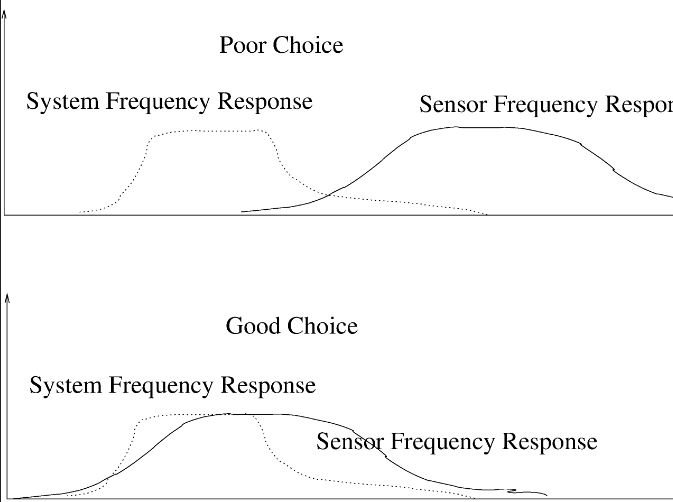
\includegraphics[scale=0.60]{day3_seg1_numerical/sensor_selection.jpg}
\end{frame}

\begin{frame}
  \onslide<1->{
	\frametitle{Kalman Filter Theory vs. Reality} 
	\framesubtitle{}
}
\begin{itemize}
  \onslide<2->{
  \item Choose sensors to match states.\\
E.g., consider the state model
\[
\begin{bmatrix}
\dot{x}_1\\
\dot{x}_2
\end{bmatrix}
= \begin{bmatrix}
0\\
0
\end{bmatrix}
\]
with the measurement model
\[
z = \begin{bmatrix} 1\;\; 0 \end{bmatrix}\begin{bmatrix}
x_1\\
x_2
\end{bmatrix}
+ v
\]
}
  \onslide<3->{
\item   Here $x_1$ is observable but $x_2$ is not, because there are no dynamic paths in $A=I$ flow infomation 
about $x_1$ into $x_2$
}
\end{itemize}
\end{frame}

\begin{frame}
  \onslide<1->{
	\frametitle{Kalman Filter Theory vs. Reality} 
	\framesubtitle{Sensor Selection}
}
\begin{itemize}
  \onslide<2->{
  \item Examine the $H$ matrix that you would use with this sensor!
}
  \onslide<3->{
  \item If it renders some states unobservable, then consider adding 
  additional sensors for those states, or replacing this sensor with one that is more favorable
}
\end{itemize}
\end{frame}
% day3_seg4_ins_challenges/observability.tex
\begin{frame}
  \onslide<1->{
	\frametitle{Observability} 
	\framesubtitle{}
}
\begin{itemize}
  \onslide<2->{
 \item Structural observability is concerned with how $H$ maps measurements into states
}
  \onslide<3->{
  \item Observability means there is a linear path from the measurements to states
}
  \onslide<4->{
  \item Structural observability determined by $\Phi$ and $H$:
}
  \onslide<5->{
\item  If $H$ is $1\times n$, where $n$ is the size of the state vector, then the state $x_0$ 
is said to be \textbf{observable }from $n$ scalar measurements $\set{z_0,\ldots,z_{n-1}}$ if the block matrix
\[
\begin{bmatrix}
H\trans&\Phi\trans H\trans & \cdots & (\Phi\trans)^{n-1}H\trans
\end{bmatrix}
\]
is of rank $n$

}
  \onslide<6->{
 \item Will making measurements as governed by $H$ actually enable us to estimate all of the states 
 in the state vector? 
}
 \end{itemize}
\end{frame}

\begin{frame}
  \onslide<1->{
	\frametitle{Observability} 
	\framesubtitle{Designing Observability into the Filter}
}
\begin{itemize}
  \onslide<2->{
  \item Observability challenge for filters is often a matter of choosing right kinds of sensors
}
  \onslide<3->{
  \item Choosing the right measurement scheduling
}
  \onslide<4->{
  \item Certain kinds of divergence can be the result of poor observability
}
  \onslide<5->{
\item   Example: Let $H=\left[1\;\;0\;\; 0\;\; 0\;\; 0\right]$, 
$\Phi=
\begin{bmatrix}
0&1&0&0&0\\
0&0&1&0&0\\
0&0&0&1&0\\
0&0&0&0&1\\
1& 2&3&4&5
\end{bmatrix}$
}
  \onslide<6->{
	\item What is the rank 
	of $\left[H\trans\;\;\Phi H\trans\;\;\Phi^2 H\trans\;\; \Phi^3 H\trans\;\;\Phi^4 H\trans\right]$?
}
\end{itemize}
\end{frame}



% day2_seg4_numerical/divergence.tex
\begin{frame}
  \onslide<1->{
	\frametitle{Filter Divergence} 
	\framesubtitle{}
}
\begin{itemize}
  \onslide<2->{
\item Kinds of Divergence
}
  \onslide<3->{
\item Causes and Remedies
}
\end{itemize}
\end{frame}

\begin{frame}
  \onslide<1->{
	\frametitle{Filter Divergence} 
	\framesubtitle{Kinds of Divergence}
}
\begin{itemize}
  \onslide<2->{
\item Mean estimation error is supposed to converge to 0
\begin{itemize}
	\item $\esterrdef$
	\item $\expect{\esterr}\rightarrow 0$
	\item Estimate is unbiased: $\expect{\hat{x}(k)}=x(k)$
\end{itemize}
}
  \onslide<3->{
\item Covariance matrix for estimation error is same as state estimation error covariance matrix: $\covmatdef$
}
\end{itemize}
\end{frame}

\begin{frame}
  \onslide<1->{
	\frametitle{Kinds of Divergence} 
	\framesubtitle{}
}
\begin{itemize}
  \onslide<2->{
\item For optimal filter, $P$ will indicate convergence or divergence.
	\begin{itemize}
		\item One common form of divergence due to round-off will send $P$ to zero
	\end{itemize}
}
  \onslide<3->{
\item For suboptimal filters, $P$ will not necessarily indicate divergence
	\begin{itemize}
	  \item $P$ may seem to indicate nominal steady-state values and yet the state estimate may go diverge from the true value
	\end{itemize}
}
\end{itemize}
\end{frame}


\begin{frame}

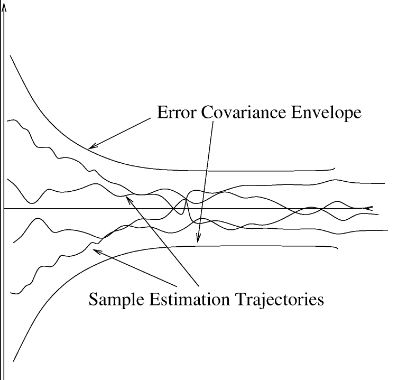
\includegraphics[scale=0.60]{day3_seg1_numerical/covconverge.jpg} 

\end{frame}


\begin{frame}
  \onslide<1->{
	\frametitle{Kinds of Divergence} 
	\framesubtitle{}
}
\begin{itemize}
  \onslide<2->{
\item Going to sleep:  error covariance becomes so small that measurements are no longer believed by the filter
}
  \onslide<3->{
\item Loss of symmetry in $P$
}
  \onslide<4->{
\item Loss of positive definiteness: negative numbers on the diagonal!
}
\end{itemize}
\end{frame}

% day2_seg4_numerical/numstab.tex
\begin{frame}
  \onslide<1->{
	\frametitle{Numerical Stability} 
	\framesubtitle{}
}
\begin{itemize}
  \onslide<2->{
 \item System stability:  Bounded input results in bounded output
}
  \onslide<3->{
 \item Numerical stability: small errors at each computation step do not grow without bound
}
  \onslide<4->{
 \item Matrix Conditioning (will address in discussing SRIF)
}
\end{itemize}
\end{frame}

%\input{day2_seg4_numerical/matrix_conditioning.tex}
% day2_seg4_numerical/roundoff.tex
\begin{frame}
  \onslide<1->{
	\frametitle{Round-Off Errors} 
	\framesubtitle{Joseph Form}
}
\begin{itemize}
  \onslide<2->{
 \item Computer round-off in floating point arithmetic
}
  \onslide<3->{
 \item Unit round-off value is largest number $\eps$ such that $1+\eps=1$
}
  \onslide<4->{
 \item In Matlab, the global symbol "eps" stores the unit round-off value
}
  \onslide<5->{
  \item Round-off errors generally plague the classical covariance update algorithm
\[\covupdateeq\]
\begin{itemize}
  \item Alternative, called the Joseph form, is more robust:
\[\josephcovupdateeq\]
\end{itemize} 
}
\end{itemize}
\end{frame}

\begin{frame}
  \onslide<1->{
	\frametitle{Round-Off Errors} 
	\framesubtitle{De Vries Mechanization}
}
\begin{itemize}
  \onslide<2->{
\item   This form in turn leads to the De Vries mechanization of the
Kalman gain equation.  To see this, first expand
the Joseph form (omitting subscripts for clarity):

}
  \onslide<3->{
\begin{align*}
   P(+)&= P(-)-KHP(-)-P(-)H\trans K\trans+ KHP(-)H\trans K\trans +
   KRK\trans.
\end{align*}
}
\end{itemize}
\end{frame}

\begin{frame}
  \onslide<1->{
	\frametitle{Round-Off} 
	\framesubtitle{De Vries}
}
\begin{itemize}
  \onslide<2->{
\item   Define
\begin{equation}\label{Feq}
  F=PH\trans
\end{equation}
and
\begin{equation}\label{Deq}
  D=HF+R.
\end{equation}

}
  \onslide<3->{
\item   We note that $D$ is symmetric, because
\begin{align*}
  D\trans &= [HF+R]\trans \\
  &= [HPH\trans + R]\trans \\
  &= [HPH\trans] \trans + R\trans \\
  &= [H\trans]\trans P\trans H\trans + R\trans \\
  &= HPH\trans + R & \text{(because $P$ and $R$ are symmetric)}\\
  &= HF + R \\
  &= D.
\end{align*}
}
\end{itemize}
\end{frame}

\begin{frame}
  \onslide<1->{
	\frametitle{Round-Off} 
	\framesubtitle{De Vries}
}
\begin{itemize}
  \onslide<2->{
\item   The gain in standard Kalman gain equation
\[\kalgaineq\] can be written as
\[K=FD^{-1}.\]
}
  \onslide<3->{
\item   Using Eqs.~(\ref{Feq}) and ~(\ref{Deq}), we compute
\begin{align*}
  P(+) &= P(-) - KF\trans - FK\trans + KDK\trans \\
  &= P(-)-K\left[F\trans - \frac{DK\trans}{2} \right] - \left[
  F-\frac{KD}{2}\right]K\trans.
\end{align*}

}
  \onslide<4->{
\item   Letting $G=F-\dfrac{KD}{2}$, we obtain
\begin{equation}\label{dvcovupdateeq}
  \dvcovupdateeq.
\end{equation}

}
\end{itemize}
\end{frame}

\begin{frame}
  \onslide<1->{
	\frametitle{Round-Off} 
	\framesubtitle{De Vries}
}
\begin{itemize}
  \onslide<2->{
\item   The De Vries mechanization implements Eq.~(\ref{dvcovupdateeq}) by
subtracting the $ij^{th}$ element of $GK\trans$ from both the
$ij^{th}$ and $ji^{th}$ elements of $P(-)$. 
}
  \onslide<3->{
\item   The De Vries form of
the covariance update equation is valid for any arbitrary gain
matrix $K$, not just the optimal gains computed from
Eqs.~(\ref{Feq}) and (\ref{Deq}).

}
\end{itemize}
\end{frame}

% day2_seg4_numerical/matinv.tex
\begin{frame}
  \onslide<1->{
	\frametitle{Numerical Stability} 
	\framesubtitle{Matrix Inversion}
}
\begin{itemize}
  \onslide<2->{
 \item Matrix inversion is always risky due to potential ill-conditioning
}
  \onslide<3->{
 \item One way to avoid this is to process measurements sequentially as scalars
}
  \onslide<4->{
 \item Or at least as low-dimensional matrices
}
\end{itemize}
\end{frame}

%% day2_seg4_numerical/symmloss.tex
\begin{frame}
Loss of Symmetry and Positive Definiteness
 \begin{itemize}
 \item
 \item
 \item
\end{itemize}
\end{frame}

% day2_seg4_numerical/exercises.tex
\begin{frame}
  \onslide<1->{
	\frametitle{Exercises} 
}
\begin{itemize}
  \onslide<2->{
\item   1. Let $v=[1\;\; -2]\trans$.  Compute the positive definite, symmetrix matrix $M=vv\trans$

}
  \onslide<3->{
\item   2. Use the following algorithm (Grewal \& Andrews) to factor $M$ into $UDU\trans$ form:
}
\end{itemize}
\end{frame}
\begin{frame}[fragile]
	\frametitle{Exercises} 
\begin{verbatim}
for j=m:-1:1
    for i=j:-1:1
        covar=P(i,j);
        for k=j+1:m
            covar=covar-U(i,k)*D(k,k)*U(j,k);
        end
        if i==j
            D(j,j)=covar;
            U(j,j)=1;
        else
            U(i,j)=covar/D(j,j);
        end
    end
end
\end{verbatim}
\end{frame}

  % Too Brief
% day3_seg1_navproblem/navproblem_main.tex
\begin{frame}
\textbf{Segment 10\\
The Navigation Problem and Reference Frames\\
Topics}
 \begin{itemize}
 \item Basic Navigation Problem
 \item Earth Referenced Navigation
 \item Coordinate Frame Conversion
 \item Basic Strapdown Navigation Equations
\end{itemize}
\end{frame}
% day3_seg1_navproblem/basicnavprob.tex
\begin{frame}
Basic Navigation Problem
 \begin{itemize}
 \item Where am I?
 \item Where am I headed?
 \item How fast am I going?
\end{itemize}
\end{frame}
\begin{frame}
Basic Navigation Problem
 \begin{itemize}
 \item What's my position?
 \item What's my heading and attitude?
 \item What's my velocity?
\end{itemize}
\end{frame}
\begin{frame}
Solution in Inertial Space
 \begin{itemize}
 \item In inertial space, it's no problem!
 \item Just integrate the acceleration once to get velocity, twice to get
 position.
\[v(T) = v(0) + \int_{0}^{T}\dfrac{d^2r}{dt^2}dt\]
\[r(T) = r(0) + \int_{0}^{T}v(T)dt\]
 \item And integrate the angular rate once to get attitude.
\end{itemize}
\end{frame}

\begin{frame}
Solution in Inertial Space
\begin{itemize}
  \item Solution easy in inertial space because ...
  \begin{itemize}
	\item inertial instruments sense acceleration and rotational rate with respect to inertial coordinate frame 
	\item inertial frame attached to sensor platform
    \item Note: You still need to rotate accelerations from body to inertial coordinates prior to integration (strapdown)
  \end{itemize}
  \item But we don't necessarily want the answer to our questions expressed in terms of inertial coordinates!
\end{itemize} 
\end{frame}

% day3_seg1_navproblem/earthrev.tex
\begin{frame}
Earth Referenced Navigation
 \begin{itemize}
 \item Terrestial navigation seeks to answer nav questions with respect to earth
 \begin{itemize}
   \item Global earth reference
   \item Local or relative navigation
 \end{itemize}
 \item Complications:
 \begin{itemize}
   \item Earth surface is curved (ellipsoid)
   \item Earth is turning (can usually ignore motion about the Sun for terrestrial nav)
 \end{itemize}
\end{itemize}
\end{frame}

% day3_seg1_navproblem/coordconv.tex
\begin{frame}
Coordinate Frames
 \begin{itemize}
 \item Inertial
 \item Earth Fixed
 \item Local Level
 \item Body
\end{itemize}
\end{frame}
\begin{frame}
Coordinate Frames
 \begin{itemize}
  \item Technically speaking, all frames are earth-centered
  \item Practically speaking, we think of the Body frame as centered in the body of the vehicle (usually at center of gravity).
  \item Local Level is thought to be located at surface of earth directly beneath the vehicle.
\end{itemize}
\end{frame}
\begin{frame}
Inertial Reference Frames
 \begin{itemize}
 \item Non-Rotating
 \item Non-Accelerating
 \item Fixed or moving uniformly with respect to another inertial
 frame (fixed stars)
\end{itemize}
\end{frame}
\begin{frame}
Inertial Reference Frames
 \begin{itemize}
 \item Nav problem "easy" in inertial frames
 \item Integrate gyro rates once to get attitude (rotational motion is absolute)
 \item Rotate accelerometer outputs to inertial frame using attitude matrix, then integrate to get inertial
 velocity; integrate velocity to get position.
 \item Would still have to contend with instrument imperfections.
\end{itemize}
\end{frame}
\begin{frame}
Inertial Reference Frame Integrations
\begin{equation}\label{inertacceleq}
\ddot{r}(t)=\specforce+\text{other external forces}
\end{equation}
\begin{equation}\label{inertveleq}
v(T)=\dot{r}(T)=v(0)+\int_{0}^{T}\specforce dt + \int_{0}^{T}(\text{other
external forces})dt
\end{equation}
\begin{equation}\label{inertposeq}
  r(T)=r(0)+\int_{0}^{T}v dt
\end{equation}
\end{frame}
\begin{frame}
Earth Fixed = ECEF = Earth Centered Earth Fixed
 \begin{itemize}
 \item Rotating frame, i.e., non-inertial
 \item Cartesian ($X,Y,Z$ in meters)
 \item Spherical (latitude $\lat$, longitude $\lon$, altitude $\alt$)
 \begin{itemize}
 \item geodetic
 \end{itemize}
\end{itemize}
\end{frame}
\begin{frame}
Local Level
 \begin{itemize}
 \item Tangent to earth's surface but translated to center of
 earth.
 \item Vertical $Z$-axis is normal to earth's surface
 \item $X,Y$-axes are level
 \item Several kinds: $Y$ north-slaved, wander (0 transport rate) or free azimuth
 \item $Y$ makes wander angle $\alpha$ with respect to true north (ENU=East, North, Up).
\end{itemize}
\end{frame}

\begin{frame}
%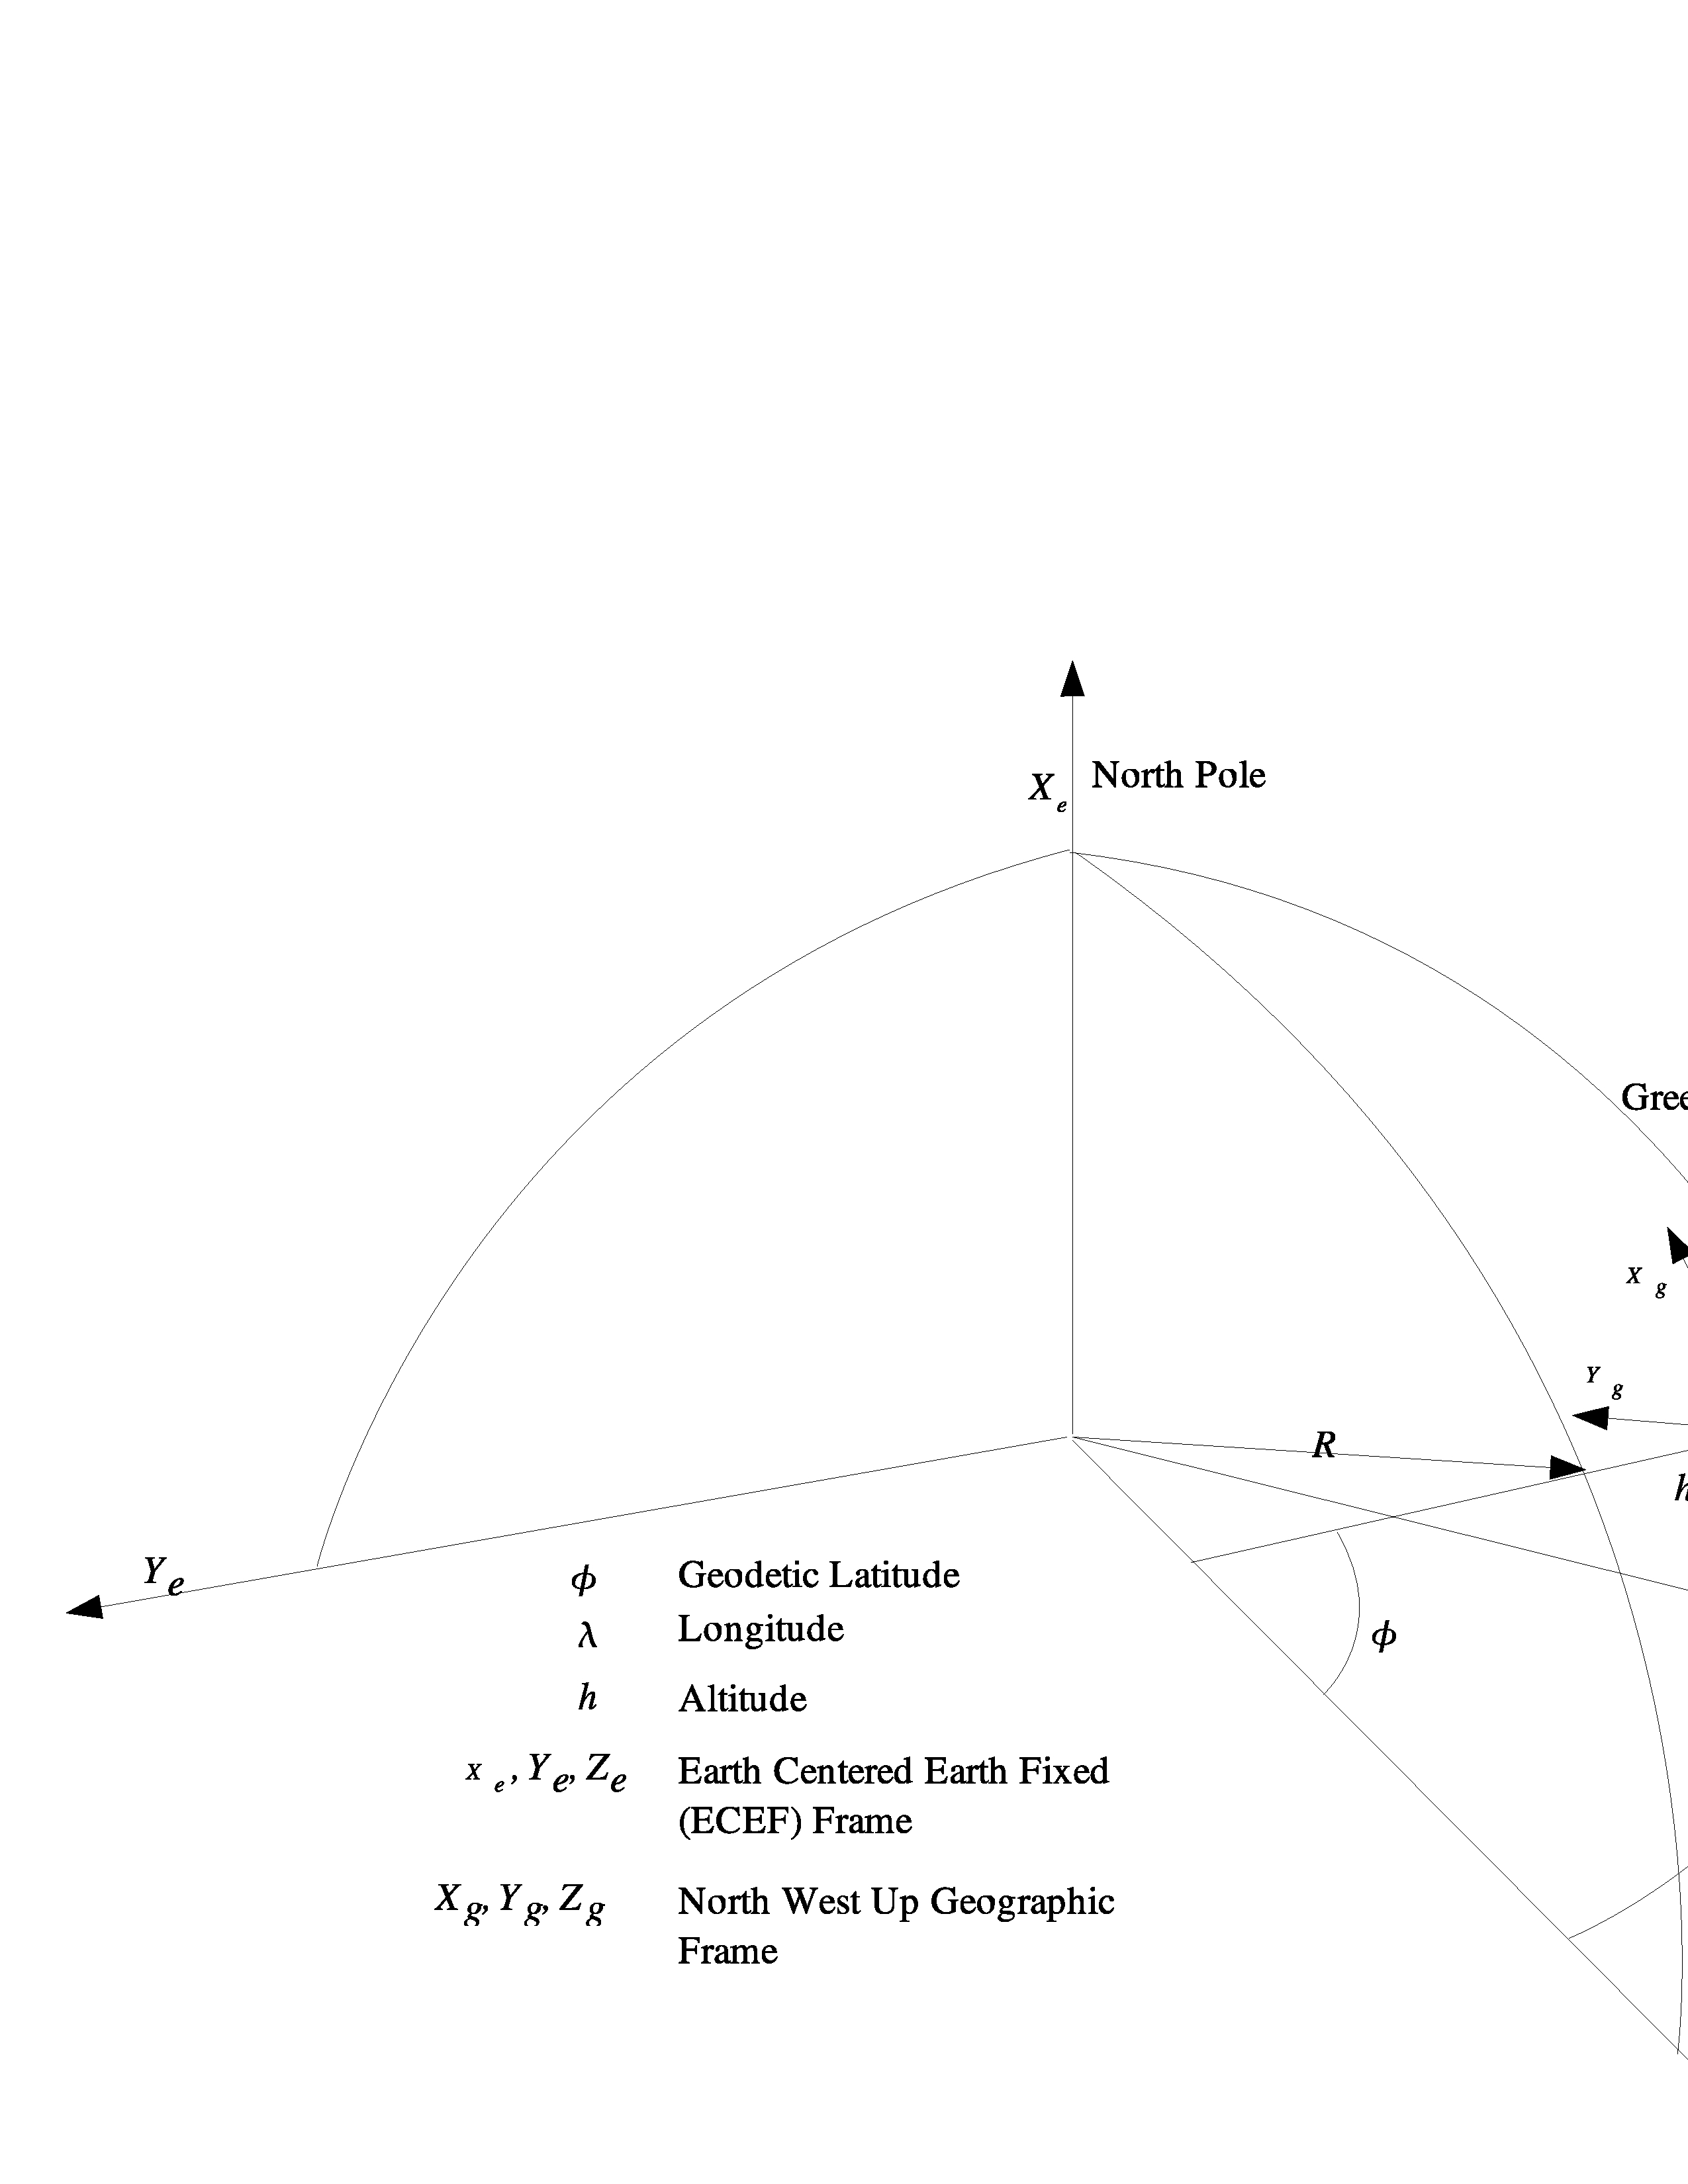
\includegraphics[width=\textwidth]{graphics/ecef.jpg}

\vfill
\end{frame}


\begin{frame}
Body Frame
 \begin{itemize}
 \item Attached to vehicle
 \item For aircraft:
   \begin{itemize}
    \item $X$ out the nose
    \item $Y$ out the right wing
    \item $Z$ down
   \end{itemize}
\end{itemize}
\end{frame}
\begin{frame}
Coordinate Frame Conversion
 \begin{itemize}
 \item All frames are earth-centered, hence differ only by
 rotation
 \item Rotation represented by direction cosine matrices (DCM)
 \begin{itemize}
	\item Represents the angles made by each of the basis vectors of one frame with those of the other
 \end{itemize}
 \item $\dcm{A}{B}$ = DCM transformation from frame A to frame B
\end{itemize}
\end{frame}
\begin{frame}
Coordinate Frame Conversion
\begin{itemize}
  \item "Direction Cosine" comes from dot product:
\[\ip{x}{y}=x\cdot y=\norm{x}\norm{y}\cos\theta_{xy}\]
where $\theta_{xy}$ is the angle between the two vectors $x$ and $y$.
  \item If $x$ and $y$ are unit vectors, then $\norm{x}=\norm{y}=1$ and we have:
\[\ip{x}{y}=x\cdot y=\cos\theta_{xy}\]
\end{itemize} 
\end{frame}

\begin{frame}
Coordinate Frame Conversion
\begin{itemize}
  \item If $U=\set{u_1,u_2,u_3}$ and $V=\set{v_1,v_2,v_3}$ are two sets of orthonormal basis vectors, then the DCM relating one frame to the other is given by:
\begin{align*}
\dcm{U}{V}&=
\begin{bmatrix}
\ip{u_1}{v_1} & \ip{u_1}{v_2} & \ip{u_1}{v_3}\\
\ip{u_2}{v_1} & \ip{u_2}{v_1} & \ip{u_2}{v_3}\\
\ip{u_3}{v_1} & \ip{u_3}{v_2} & \ip{u_3}{v_3}\\
\end{bmatrix}\\
&=
\begin{bmatrix}
\cos\theta_{11} & \cos\theta_{12} & \cos\theta_{13}\\
\cos\theta_{21} & \cos\theta_{22} & \cos\theta_{23}\\
\cos\theta_{31} & \cos\theta_{32} & \cos\theta_{33}\\
\end{bmatrix}
\end{align*}
\end{itemize} 
\end{frame}

\begin{frame}
Coordinate Frame Conversion
 \begin{itemize}
 \item DCMs are orthogonal matrices $\Rightarrow \left[\dcm{A}{B} \right]^{-1}=\left[\dcm{A}{B} \right]\trans$
 \item Third row (or column) is vector cross product of other two\\
 $\Rightarrow$ only six independent parameters
 \item DCMs satisfy:   $\dcm{B}{A}\dcm{C}{B}=\dcm{C}{A}$
\end{itemize}
\end{frame}
\begin{frame}
Coordinate Frame Conversion: Most important DCMs
 \begin{itemize}
 \item Body to Local Level: $\dcm{B}{L}$
 \begin{itemize}
 \item sometimes called Body to Nav and notated $\dcm{B}{N}$
 \item yields attitude info (Euler angles for roll, pitch, yaw)
 \end{itemize}
 \item Local Level to Earth: $\dcm{L}{E}$
 \begin{itemize}
 \item yields position info and also used to transform earth rate to
 local level
 \end{itemize}
\end{itemize}
\end{frame}
\begin{frame}
Coordinate Frame Conversion: Most important DCMs
\begin{itemize}
  \item Visualize $\dcm{L}{E}$'s determination of position as follows:
	\begin{itemize}
		\item As vehicle moves, local level frame changes its orienation with respect to earth's center in order to maintain local level with respect to earth's surface
		\item If you think of local level frame as attached to earth's surface, you get distracted by the displacement of the frame
		\item If you move local level frame to center of earth, the displacement disappears and all that remains are the rotations
	\end{itemize} 
\end{itemize} 
\end{frame}

\begin{frame}

%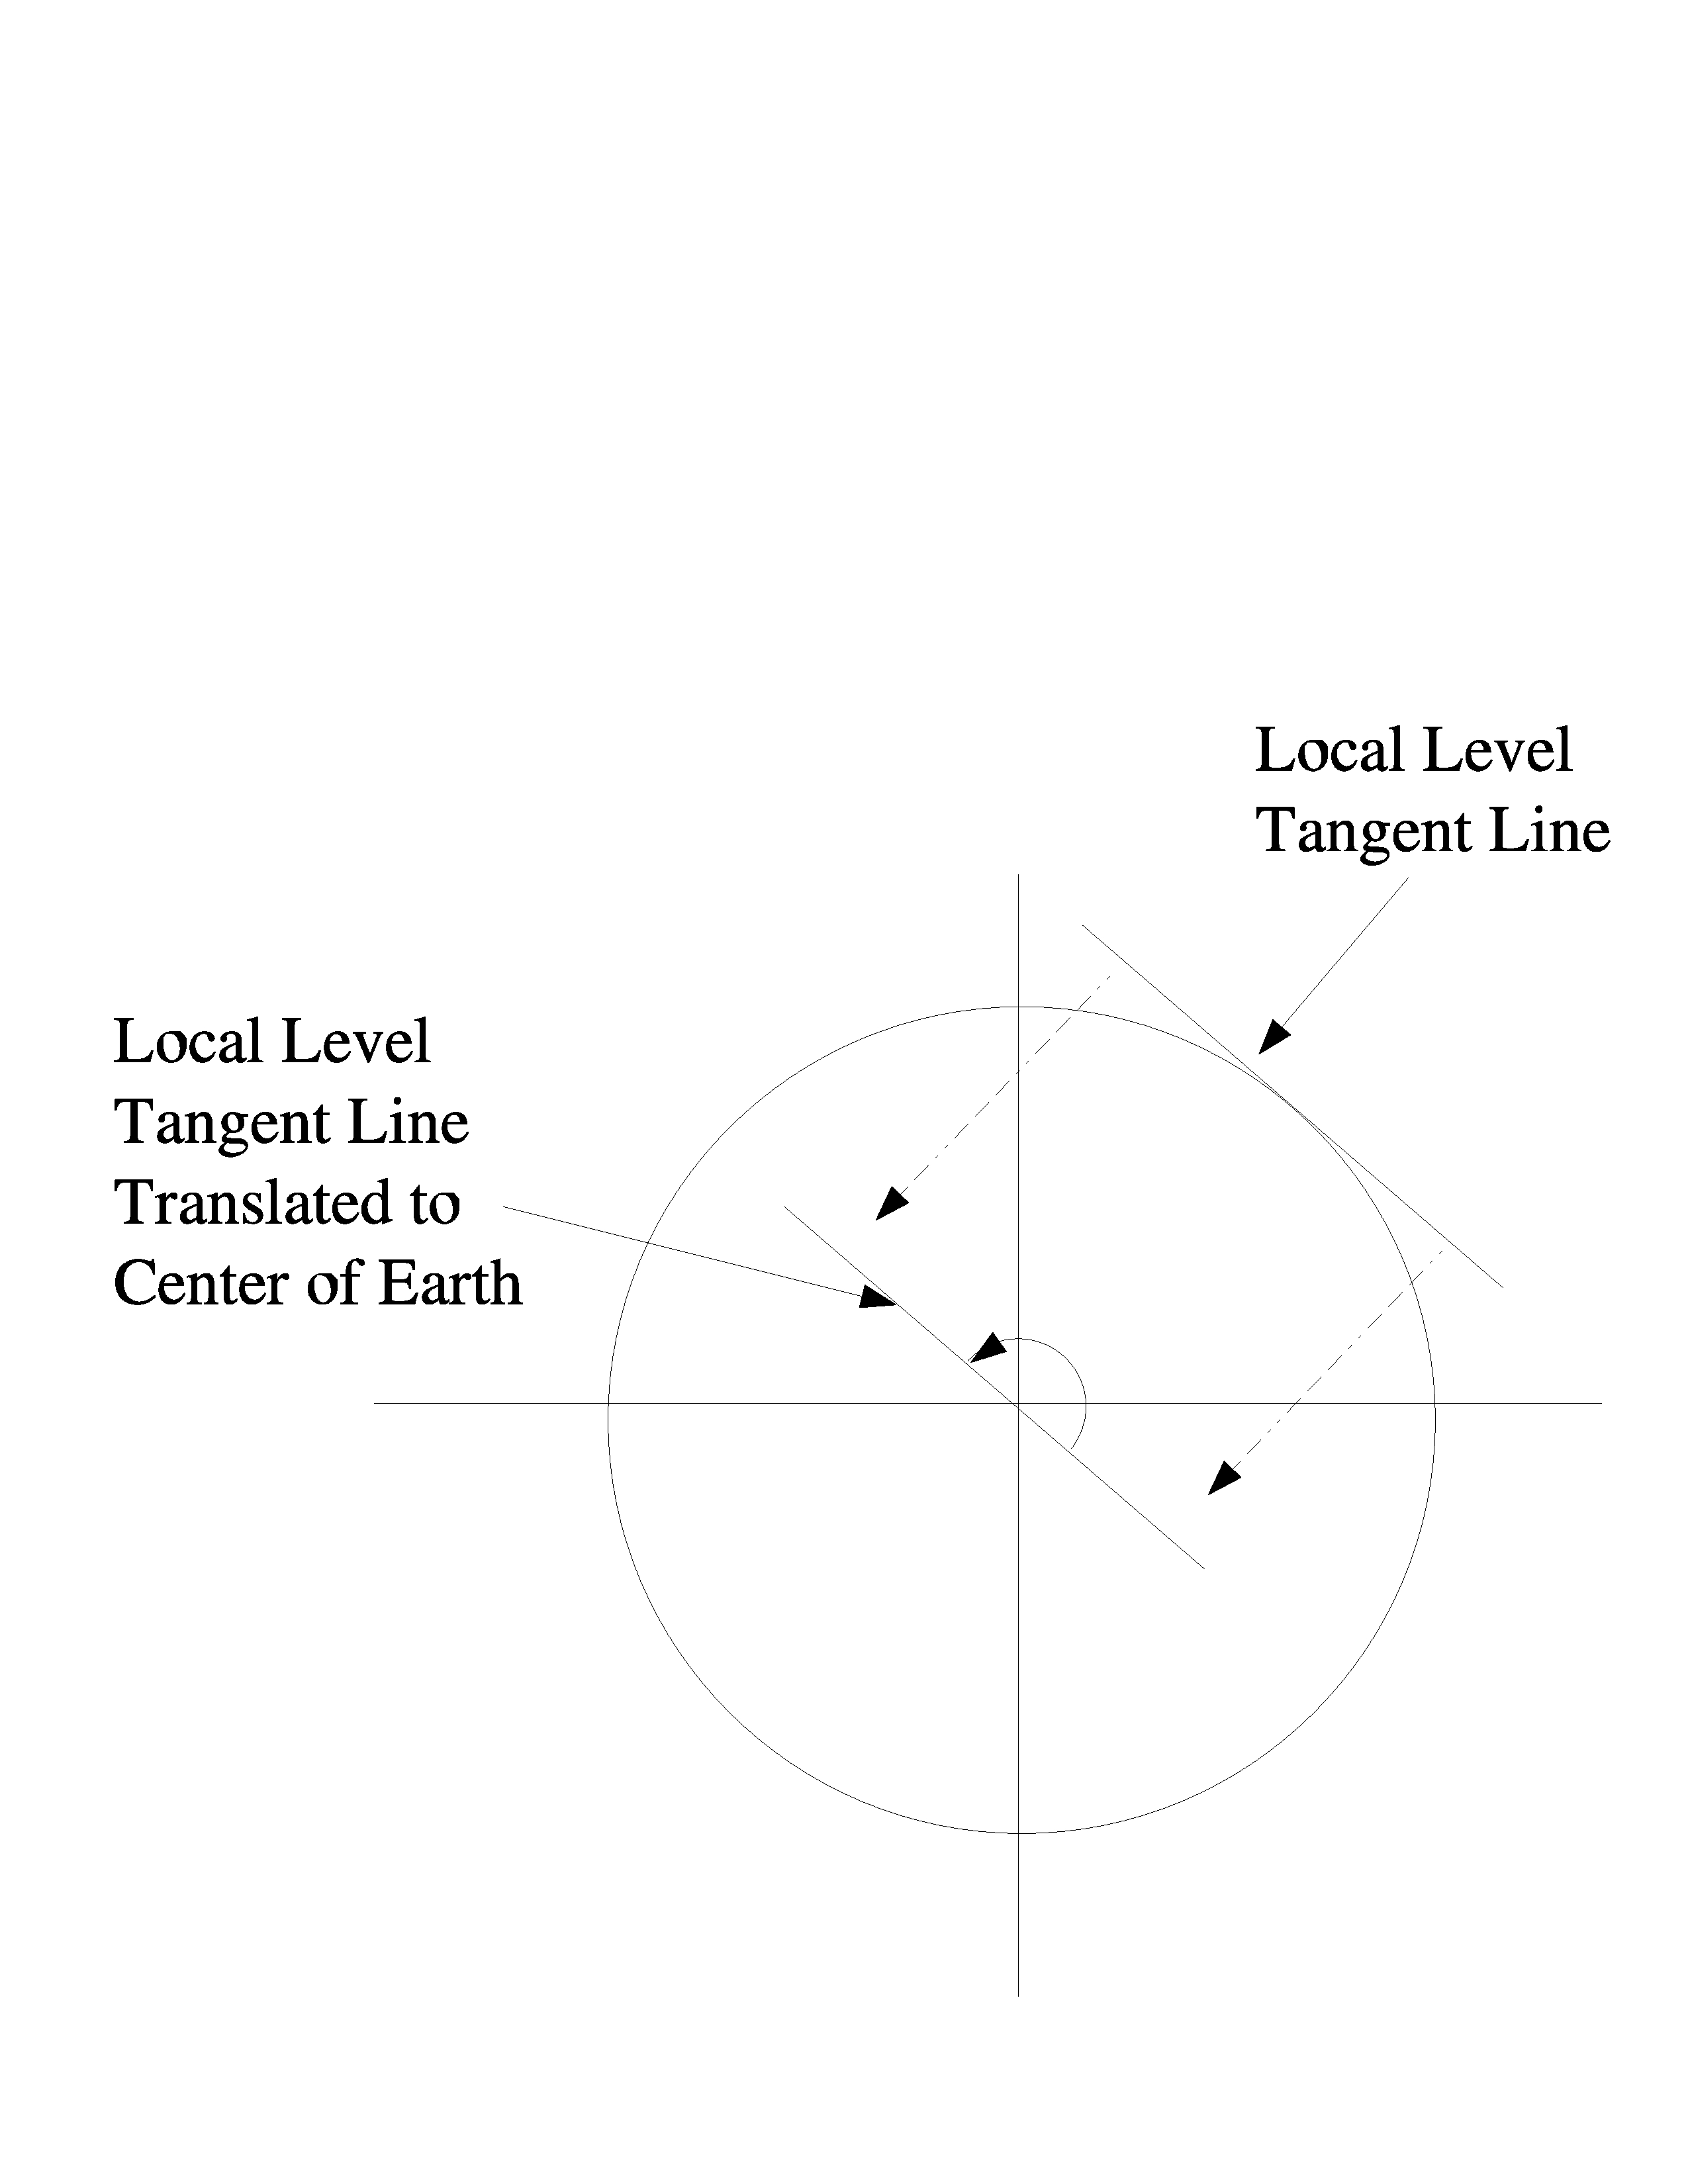
\includegraphics[width=\textwidth]{day3_seg2_navproblem/pos_dcm.jpg}

\end{frame}
% day3_seg1_navproblem/strapdown.tex
\begin{frame}
Strapdown Navigation:  Strapdown vs. Gimbaled
\begin{itemize}
  \item Gimbaled INS:
  \begin{itemize}
	\item Gyro stabilized platform
	\item Gimbal assembly and torque motors
	\item Resolvers, slip rings, bearings, etc. to control  platform
	\item Goal: Maintain stable, locally level or inertial reference frame
  \end{itemize}
\end{itemize} 
\end{frame}


\begin{frame}
Strapdown Navigation: Strapdown vs. Gimbaled
\begin{itemize}
  \item Gimbaled INS Issues
  \begin{itemize}
	\item Reliability and Cost: Lots of moving parts!
	\item Body rate and acceleration information not directly available
	\item Rate signals are generally noisy and have low bandwidth
  \end{itemize}
\end{itemize} 
\end{frame}


\begin{frame}
Strapdown Navigation: Strapdown vs. Gimbaled
\begin{itemize}
  \item Strapdown INS:
  \begin{itemize}
	\item Inertial instruments strapped to body frame
	\item Requires local level accelerations to be computed using direction cosine matrix $\dcm{B}{L}$
	\item $\dcm{B}{L}$ derived from gyro-sensed body rates
    \item Strapdown systems can be implemented with either rate gyros or attitude gyros 
  \end{itemize} 
\end{itemize} 
\end{frame}

\begin{frame}
Strapdown Navigation: Strapdown vs. Gimbaled
\begin{itemize}
  \item Strapdown INS Advantages
  \begin{itemize}
	\item Immediate detection of body rates and accelerations
	\item Fewer moving parts
	\item Potential redundancy advantages
  \end{itemize} 
  \item Gimbaled systems are nearly obsolete
\end{itemize} 
\end{frame}

\begin{frame}
%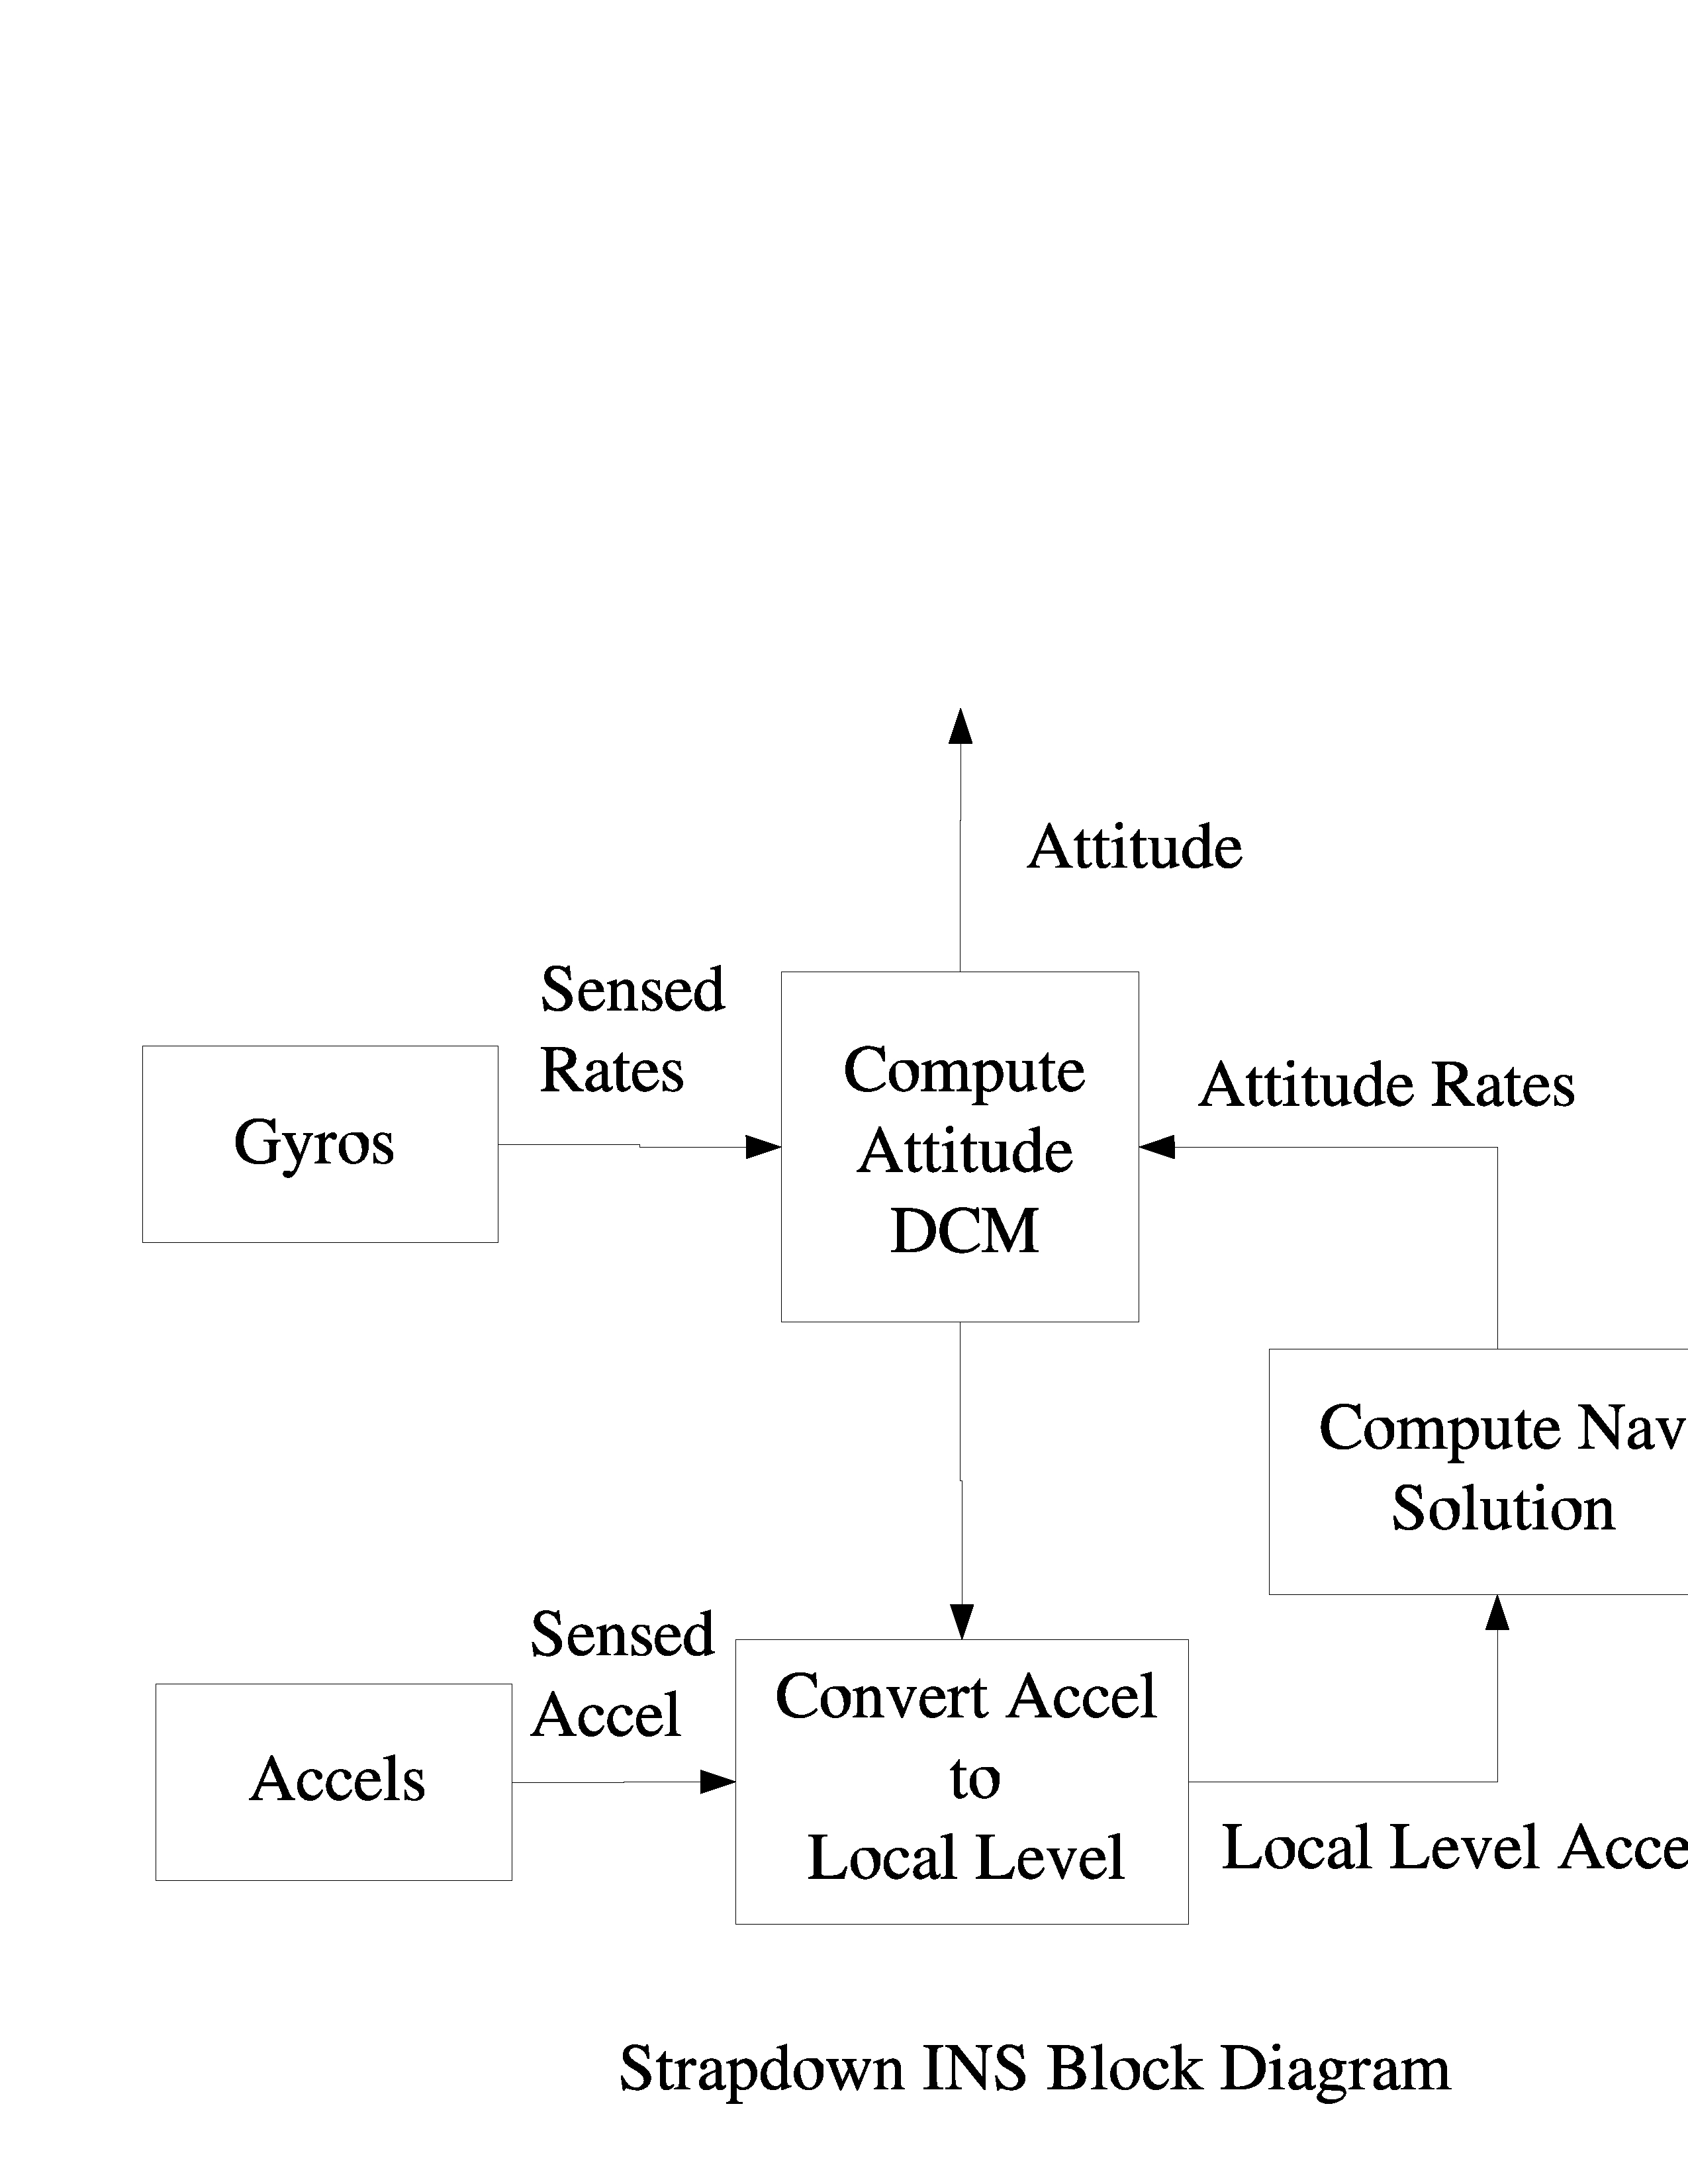
\includegraphics[width=\textwidth]{graphics/strapdown_block.jpg}
\end{frame}

\begin{frame}
Basic Strapdown Navigation Equations
 \begin{itemize}
 \item Need to compute attitude, velocity, and position
 \item I.e., need to compute $\dcm{B}{L}$ and $\dcm{L}{E}$
 \item These DCMs are dynamic quantities
 \item $\dcm{B}{L}$ determines attitude and can be rapidly varying
 \item $\dcm{L}{E}$ determines position and is slowly varying (relative to attitude dynamics)
\end{itemize}
\end{frame}

\begin{frame}
Rotating Coordinate Frames
\begin{itemize}
\item We first need to understand how an arbitrary vector and its time
derivatives in one coordinate frame are expressed in another frame
that is rotating with respect to the first.  
\item Let $A$ and $B$
denote two coordinate frames and assume that $B$ is rotating with
respect to $A$.  
\item We use the notation $\rotvec{A}{B}^A$ to express
the direction and magnitude of the rotation vector as seen in the $A$ frame.
\end{itemize}
\end{frame}
\begin{frame}
Rotating Coordinate Frames
\begin{itemize}
\item Every rotation vector can also be expressed as a skew symmetric
matrix.  
\item If $\omega$ is a rotation vector (without mentioning the
frames involved), then
\[\Omega = \skewsymmat{\omega}{1}{2}{3}.\]
\end{itemize}
\end{frame}
\begin{frame}
Rotating Coordinate Frames
\begin{itemize}
\item Since multiplication of a vector by the skew symmetric matrix
equivalent is the same thing as left multiplying the cross product
of the original vector, we can write:
\[\Omega v = \omega \times v\]
\item Therefore the notation $\xop{\omega}=\Omega$ is
common\footnote{One must be careful in making this identification
since left matrix multiplication is associative while left cross
product multiplication is not.}
\end{itemize}
\end{frame}

\begin{frame}
Rotating Coordinate Frames
\begin{itemize}
\item Let $v$ be an arbitrary vector in 3-space. 
\item Let
$\set{e_A^1,e_A^2,e_A^3}$ be orthonormal basis vectors in the $A$
frame 
\item Let $\set{e_B^1,e_B^2,e_B^3}$ be orthonormal basis
vectors in the $B$ frame\footnote{We reverse the roles of superscripts
and subscripts for basis vectors so that we may employ the
Einstein summation convention on occasion.}.  
\end{itemize}
\end{frame}

\begin{frame}
Rotating Coordinate Frames
\begin{itemize}
\item Thus, we can write
$v$ as $\sum_{i=1}^3 v_i^A e_A^i$ and also $\sum_{i=1}^3 v_i^B
e_B^i$. 
\item This is one and the same vector expressed in two different
coordinate frames\footnote{A vector is a linear combination of
basis vectors and not necessarily an ordered triple of real numbers.}.
\end{itemize}
\end{frame}
\begin{frame}
Rotating Coordinate Frames
\begin{itemize}
\item Note that, with respect to an arbitrary inertial
reference frame, we have for the time derivative:
\begin{align*}
  v &= \sum_{i=1}^3 v_i^A e_A^i = \sum_{i=1}^3 v_i^B e_B^i\\
    &\Rightarrow  \dot{v} = \dfrac{d}{dt}\left[ \sum_{i=1}^3 v_i^A e_A^i \right] = \dfrac{d}{dt}\left[\sum_{i=1}^3 v_i^B e_B^i
    \right]\\
    &\Rightarrow \sum_{i=1}^3 \left( \dot{v}_i^A e_A^i+ v_i^A
    \dot{e}_A^i\right)
    = \sum_{i=1}^3 \left(\dot{v}_i^B e_B^i+ v_i^B \dot{e}_B^i\right)\\
\end{align*}
\end{itemize}
\end{frame}
\begin{frame}
Rotating Coordinate Frames
\begin{itemize}
\item In the special case
that their respective coordinate frames are not rotating relative
to one another, each $\dot{e}_A^i = 0 = \dot{e}_B^i$.   
\item Nevertheless, regardless of rotation, we must always have:
\begin{equation}\label{scalarinveq}
  \scalarinveq.
\end{equation}
(Note that, in general, $\dot{v}_i^A\neq\dot{v}_i^B$.)
\end{itemize}
\end{frame}
\begin{frame}
Rotating Coordinate Frames
\begin{itemize}
\item Let frame $B$ rotate with respect to frame $A$ at a constant
rotational rate $\rotvec{A}{B}^A$ as expressed in $A$ frame coordinates.  
\item Since $B$ is not rotating with respect to itself, let us agree to label the quantity in Eq. \eqref{scalarinveq} as
$\dot{v}^B$. 
\item We'll assume that $A$ is an inertial frame and thus $\dot{v}=\dot{v}^A$.
\end{itemize}
\end{frame}
\begin{frame}
Rotating Coordinate Frames
\begin{itemize}
\item When viewed from the $A$ frame, however, it is not true that each
of the $\dot{e_i}^B$ is zero, since these unit vectors are slaved
to the $B$ frame and $B$ is rotating with respect to $A$ at rate
$\rotvec{A}{B}^A$.  
\item Therefore, we have:
\begin{equation}\label{aderiv}
\begin{split}
\dot{v}^A&=\sum_{i=1}^3 \dot{v}_i^A e_A^i + \sum_{i=1}^3 v_i^B
\dot{e}_B^i\\
         &=\sum_{i=1}^3 \dot{v}_i^B e_B^i + \sum_{i=1}^3 v_i^B
\dot{e}_B^i \text{\;\;\;\;(by Eq. \eqref{scalarinveq})}\\
         &=\dot{v}^B +\sum_{i=1}^3 v_i^B\dot{e}_B^i.
\end{split}
\end{equation}
\end{itemize}
\end{frame}

\begin{frame}
Rotating Coordinate Frames
\begin{itemize}
\item The last sum on the right side of Eq. \eqref{aderiv} can be
rewritten as the cross product $\rotvec{A}{B}^A\times v$, because
$\dot{e}_B^i=\rotvec{A}{B}^A\times e_B^i$, and
\begin{align*}
   \sum_{i=1}^3 v_i^B\dot{e}_B^i &= \sum_{i=1}^3 v_i^B\rotvec{A}{B}^A\times e_B^i \\
  &=\rotvec{A}{B}^A\times \sum_{i=1}^3 v_i^B e_B^i \\
  &=\rotvec{A}{B}^A\times v.
\end{align*}
\end{itemize}
\end{frame}
\begin{frame}
Rotating Coordinate Frames
\begin{itemize}
\item We thus arrive at the all-important Coriolis Equation which is
used often in navigation analysis:
\begin{equation}\label{corioliseq}
  \corioliseq.
\end{equation}
\end{itemize}
\end{frame}
\begin{frame}

Alternatively, we can express Eq. \eqref{corioliseq} in
skew-symmetric matrix form using
$\rotmat{A}{B}=\xop{\rotvec{A}{B}}$:
\begin{equation}\label{coriolismateq}
  \coriolismateq.
\end{equation}

Note that we must use superscripts on both $\rotmat{A}{B}$ and $v$
as soon as we make a commitment to a particular coordinate frame
representation.\footnote{Since matrices are defined in terms of
their action on basis vectors, it is appropriate to specify the
coordinate system.  On the other hand, if $\rotmat{A}{B}$ is taken
to be a linear transformation, then superscripts are not
necessary.}.

\end{frame}


\begin{frame}
Strapdown Navigation Equations
 \begin{itemize}
 \item Three differential equations
 \begin{itemize}
   \item Equation for body to local level transformation $\dcm{B}{L}$
   \item Equation for velocity (uses $\dcm{B}{L}$)
   \item Equation for local level to earth for position DCM $\dcm{L}{E}$
 \end{itemize}
\end{itemize}
\end{frame}
\begin{frame}
Strapdown Navigation Equations
 \begin{itemize}
 \item Two Algebraic Equations
 \begin{itemize}
   \item Equation for converting velocity to transport rate (to be explained)
   \item Equation for converting earth rate to local level
   coordinates
 \end{itemize}
\end{itemize}
\end{frame}
\begin{frame}
Strapdown Navigation Equations\\
The Three Differential Equations\\
\begin{equation}\label{cbleq}
  \cbleq
\end{equation}
\begin{equation}\label{strapveleq}
  \strapveleq
\end{equation}
\begin{equation}\label{cleeq}
  \cleeq
\end{equation}
\end{frame}
\begin{frame}
Strapdown Navigation Equations\\
The Two Algebraic Equations\\
\begin{equation}\label{trateeq}
  \trateeq \text{ (wander azimuth $\rho_z=0$)}
\end{equation}
\begin{equation}\label{erateeq}
  \erateeq
\end{equation}
\end{frame}
\begin{frame}
Strapdown Navigation Equations\\
The $\dcm{B}{L}$ Equation \eqref{cbleq}
\[\cbleq\]
\begin{itemize}
\item All the $\Omega$ matrices represent rotation vector cross products in skew-symmetric matrix format
\begin{itemize}
 \item $\rotmat{I}{B}^B$ is rotational rate of aircraft in body
coordinates
\item $\rotmat{I}{E}^L$ is earth rate in local level coordinates
\item $\rotmat{E}{L}^L$ is transport rate in local level
coordinates
\end{itemize}
\end{itemize}
\end{frame}
\begin{frame}
Strapdown Navigation Equations: Detour into Cross Product Matrices\\
\begin{itemize}
\item The cross product of $\omega=\colvecthree{\omega}{}$ with any other vector $v$ is the same as multiplying $v$ on the left by
$\Omega = \skewsymmat{\omega}{1}{2}{3}$
\item $\omega \times v=\Omega v$
\end{itemize}
\end{frame}
\begin{frame}
Strapdown Navigation Equations\\
The $\dcm{B}{L}$ Equation \eqref{cbleq}
\[\cbleq\]
\begin{itemize}
\item Transport rate is the rotational rate of the aircraft due to
motion over the surface of the earth.  Is a function of velocity.
\item $\rotmat{I}{B}^B$ is total inertial angular rate sensed by gyros and includes effects of
transport and earth rates.
\item Hence transport and earth rate effects have to be subtracted
off.
\end{itemize}
\end{frame}
\begin{frame}
Strapdown Navigation Equations\\
The Strapdown Velocity Equation \eqref{strapveleq}
\[\strapveleq\]
 \begin{itemize}
 \item Sometimes referred to as the velocity rate equation
 \item $\specforce^B$ is specific force sensed by accelerometers in
 body coordinates (because the accels are strapped to the body --
 hence the term strapdown)
\end{itemize}
\end{frame}
\begin{frame}
%\includegraphics[width=10in,height=6.5in]{strapnav_block.jpg}
\end{frame}
\begin{frame}
Strapdown Navigation Equations\\
The Transport Rate Equation \eqref{cleeq}
\[\cleeq\]
\begin{itemize}
  \item Connected to velocity rate equation by the first algebraic equation \eqref{trateeq}:
\[\trateeq\]
  \item Eq. \eqref{cleeq} Sometimes referred to as position rate equation, because $\dcm{L}{E}$ directly implies the vehicle position
\end{itemize} 
\end{frame}

\begin{frame}
Strapdown Navigation Equations\\
Position Rate / Transport Rate Equations (Geographic)
\begin{itemize}
  \item North transport rate:
\begin{equation}\label{trateneq}
\trateneq
\end{equation} 
  \item East transport rate:
\begin{equation}\label{trateeeq}
\trateeeq
\end{equation} 
where $e$ is ellipticity (approx. $\dfrac{1}{298}$) and $R_e$ is mean equatorial earth radius
\end{itemize} 
\end{frame}

\begin{frame}
Strapdown Navigation Equations\\
Position Rate / Transport Rate Equations (Geographic)
\begin{itemize}
  \item Latitude Rate:
\begin{equation}\label{latrate}
\latrateeq
\end{equation}  
  \item Longitude Rate:
\begin{equation}\label{lonrate}
\lonrateeq
\end{equation}  
\end{itemize} 
\end{frame}

\begin{frame}
Strapdown Navigation Equations\\
\begin{itemize}
  \item Geographic (north-slaved) mechanization has singularities at poles
  \item Two other approaches to local level coordinates:
  \begin{itemize}
	\item Free azimuth: vertical component of transport rate $\rho_z$= additive inverse of vertical component of earth rate
	\item Wander Azimuth:  vertical component of transport rate $\rho_z$ = 0
  \end{itemize}
\end{itemize} 
\end{frame}

\begin{frame}
Strapdown Navigation Equations\\
Position Rate / Transport Rate Equations (Wander and Free Azimuth)
\begin{itemize}
  \item X Transport Rate:
\begin{align}\label{xtrateeq}
\xtrateeq
\end{align}  
  \item Y Transport Rate:
\begin{align}\label{ytrateeq}
\ytrateeq
\end{align}  
\end{itemize} 
\end{frame}

\begin{frame}
Strapdown Navigation Equations\\
Position Rate / Transport Rate Equations (Wander and Free Azimuth)
\begin{itemize}
  \item Azimuth Rate:
\[
\rho_z= 
\begin{cases} 
-\erate d_{23}, &\text{if free azimuth;}\\ 
0,  &\text{if wander azimuth} 
\end{cases}
\]
  \item In equations above, the matrix $\left[d_{ij}\right]$ is the direction cosine matrix $\dcm{L}{E}$ from local level (L) frame to earth centered earth fixed (E) frame.
\end{itemize} 
\end{frame}

% day3_seg1_navproblem/exercises.tex
\begin{frame}
Exercises\\

1.  Compute direction cosine matrix $\dcm{U}{V}$, where 
\[U=\set{(1,0,0),(0,1,0),(0,0,1)}\] 
and \[V=\set{(-1,0,0),(0,1,0),(0,0,-1)}\]

2. Suppose you are starting at the equator and travelling due north, and your velocity is 5 m/sec.  Compute the transport rates $\rho_n$ and $\rho_e$ associated with this velocity and heading.  You may use the following constants: $\erateval$ and $\eradiusval$
\end{frame}


% day3_seg2_inertial/inertial_main.tex
\begin{frame}
  \onslide<1->{
	\frametitle{Inertial Error Dynamics} 
	\framesubtitle{Topics}
}
\begin{itemize}
  \onslide<2->{
 \item Imperfect Inertial Instruments
}
  \onslide<3->{
 \item From Strapdown Equations to Error Equations
}
  \onslide<4->{
 \item Initialization: Alignment
}
\end{itemize}
\end{frame}
% day3_seg2_inertial/impinst.tex
\begin{frame}
  \onslide<1->{
	\frametitle{Inertial Error Dynamics} 
	\framesubtitle{Imperfect Inertial Instruments}
}
\begin{itemize}
  \onslide<2->{
 \item Accelerometers and Gyros have inherent imperfections
}
  \onslide<3->{
 \item Bias, scale factor, $g^2$ terms, noise, random walks, etc.
}
  \onslide<4->{
 \item Inertial sensor clusters also have errors: misalignments
}
  \onslide<5->{
 \item Many error sources are calibrated out using rate tables during ATP
}
 \onslide<6->{ 
 \item Residual effects will influence strapdown nav equations
}
\end{itemize}
\end{frame}

\begin{frame}
  \onslide<1->{
	\frametitle{Inertial Error Dynamics} 
	\framesubtitle{Imperfect Inertial Instruments}
}
\begin{itemize}
  \onslide<2->{
  \item Strapdown nav equations very sensitive to gyro errors
}
  \onslide<3->{
  \item Gyro biases yield erroneous $\dcm{B}{L}$ matrix which in turn causes erroneous accelerations to be computed in local level frame
}
  \onslide<4->{
  \item Thus, gyro errors affect not only attitude, but also position and velocity
}
\end{itemize}
\end{frame}

\begin{frame}
  \onslide<1->{
	\frametitle{Inertial Error Dynamics} 
	\framesubtitle{Simple Inertial Error Models}
}
\begin{itemize}
  \onslide<2->{
  \item Gyros
\[
\simprateerreq{x}{y}{z}
\]
\[
\simprateerreq{y}{z}{x}
\]
\[
\simprateerreq{z}{x}{y}
\]

where $\gyrobias{i}$ is the $i^\text{th}$ gyro bias, $\gyrosf{i}$ the $i^\text{th}$ gyro scale factor, and $\gyromisalign{i}{j}$ is the misalignment of the $i^\text{th}$ gyro axis toward the $j^\text{th}$ gyro axis. 
}
\end{itemize}
\end{frame}

\begin{frame}
  \onslide<1->{
	\frametitle{Inertial Error Dynamics} 
	\framesubtitle{Simple Inertial Error Models}
}
\begin{itemize}
  \onslide<2->{
  \item Accelerometers
\[
\simpaccelerreq{x}{y}{z}
\]
\[
\simpaccelerreq{y}{z}{x}
\]
\[
\simpaccelerreq{z}{x}{y}
\]
where $\accelbias{i}$ is the $i^\text{th}$ accelerometer bias, $\accelsf{i}$ the $i^\text{th}$ accelerometer scale factor, and $\accelmisalign{i}{j}$ is the misalignment of the $i^\text{th}$ accelerometer axis toward the $j^\text{th}$ accelerometer axis. 
}
\end{itemize}
\end{frame}


\begin{frame}
  \onslide<1->{
	\frametitle{Inertial Error Dynamics} 
	\framesubtitle{Bias Models}
}
\begin{itemize}
  \onslide<2->{
  \item Bias in both types of instruments can be further broken down into several components:
  \begin{itemize}
	\item fixed bias -- constant from turn-on to turn-on -- should be calibrated out
	\item bias stability -- varies from turn-on to turn-on -- can't be calibrated out, but can be characterized in terms of variance -- can model as random constant
	\item bias drift -- usually modeled as random walk
  \end{itemize} 
}
\end{itemize}
\end{frame}


\begin{frame}
  \onslide<1->{
	\frametitle{Inertial Error Dynamics} 
	\framesubtitle{Scale Factor Models}
}
\begin{itemize}
  \onslide<2->{
  \item Scale factor can also be modeled as a sum of three components
}
  \onslide<3->{
  \item Often in nav filters, scale factor residual is modeled as a random constant
}
  \onslide<4->{
  \item Important to keep in mind that the contribution of scale factor error is a function of input (rate or acceleration) 
}
\end{itemize}
\end{frame}
\begin{frame}
  \onslide<1->{
	\frametitle{Inertial Error Dynamics} 
	\framesubtitle{Higher Order Models}
}
\begin{itemize}
  \onslide<2->{
  \item In expanding the output error as a Taylor series function of input, bias, scale factor, and misalignment show up as zero and first order terms.
}
  \onslide<3->{
  \item Higher order terms are also present, especially second order terms.
}
  \onslide<4->{
  \item In some calibration and alignment filters, such higher order effects are modelled
}
  \onslide<5->{
  \item SNU-84-1 includes error budgets associated with all the combined, higher order effects.  
}
\end{itemize}
\end{frame}

\begin{frame}
  \onslide<1->{
	\frametitle{Inertial Error Dynamics} 
	\framesubtitle{Higher Order Models:  Taylor Series of Two Variables}
}
  \onslide<2->{
\begin{align*}
\gentaylordouble{f}{x}{y}{x_0}{y_0}
\end{align*}
Taylor Series provides basis for all error analysis.
}
\end{frame}

\subsection{Strapdown Error Dynamics}
% day3_seg2_inertial/straperr.tex
\begin{frame}
  \onslide<1->{
	\frametitle{Inertial Error Dynamics} 
	\framesubtitle{From Strapdown Equations to Error Equations}
}
\begin{itemize}
  \onslide<2->{
 \item Nav equations require perfect inertial instruments
}
  \onslide<3->{
 \item Instruments are not perfect
}
  \onslide<4->{
 \item Inertial instrument error sources (bias, scale factor errors, etc.) generate erroneous rate and acceleration inputs to the nav equations  
}
  \onslide<5->{
 \item Need to figure out the effects on the outputs of these equations
}
\end{itemize}
\end{frame}
% cm_kf_talk_straperr.tex


\begin{frame}
  \onslide<1->{
	\frametitle{Inertial Error Dynamics} 
	\framesubtitle{Strapdown Error Equations}
}
\begin{itemize}
  \onslide<2->{
 \item Nature of Errors
}
  \onslide<3->{
 \item Error Operator
}
  \onslide<4->{
 \item Error Equations
}
\end{itemize}
\end{frame}


\begin{frame}
  \onslide<1->{
	\frametitle{Inertial Error Dynamics} 
	\framesubtitle{Strapdown Error Equations: Nature of Errors}
}
\begin{itemize}
  \onslide<2->{
 \item Errors propagate according to derived equations
}
  \onslide<3->{
 \item Errors are generally small, so approximating assumptions
 help simplify the math
 \begin{itemize}
}
  \onslide<4->{
 \item linearize otherwise non-linear dynamics
}
  \onslide<5->{
 \item small angle assumptions:  $\sin\theta \approx \theta$
 \end{itemize}
}
\end{itemize}
\end{frame}


\begin{frame}
  \onslide<1->{
	\frametitle{Inertial Error Dynamics} 
	\framesubtitle{Strapdown Error Equations: Error Operator}
}
\begin{itemize}
  \onslide<2->{
\item   If $A$ is any quantity, we define error operator as follows:
\begin{equation}\label{errop}
  \errop{A},
\end{equation}
where $A$ is the true quantity of interest and $\hat{A}$ is an
apparent quantity.  The latter could be a measured value, and
estimated value, or some computed value.  This means that
\[\hat{A}=A+\delta A\]
i.e., the apparent value is the true value plus some error.

}
\end{itemize}
\end{frame}


\begin{frame}
  \onslide<1->{
	\frametitle{Inertial Error Dynamics} 
	\framesubtitle{Strapdown Error Equations: Error Operator}
}
\begin{itemize}
  \onslide<2->{
\item   Error operator satisfies:
\begin{equation}\label{erropid}
  \delta(AB) = \delta A \cdot B + A \cdot \delta B
\end{equation}
}
  \onslide<3->{
\item   Proof:
\begin{align*}
\delta(AB) &= \widehat{AB} - AB\\
&= \hat{A}\hat{B}-AB\\
&= (A+\delta A)(B+\delta B)-AB\\
&= AB + A\cdot\delta B +\delta A \cdot B + \delta A \cdot \delta B - AB\\
& = \delta A \cdot B + A\cdot\delta B
\end{align*}
since we may assume that $\delta A \cdot\delta B \approx 0$.
}
\end{itemize}
\end{frame}


\begin{frame}
  \onslide<1->{
	\frametitle{Inertial Error Dynamics} 
	\framesubtitle{Strapdown Error Equations}
}
\begin{itemize}
  \onslide<2->{
\item   Applying these to the three differential equations, yields three
error equations:
\begin{equation}\label{cblerreq}
  \cblerreq
\end{equation}
\begin{equation}\label{strapvelerreq}
  \strapvelerreq
\end{equation}
\begin{equation}\label{cleerreq}
  \cleerreq
\end{equation}
}
\end{itemize}
\end{frame}



\begin{frame}
  \onslide<1->{
	\frametitle{Inertial Error Dynamics} 
	\framesubtitle{Strapdown Error Equations}
}
\begin{itemize}
  \onslide<2->{
\item   Introducing \textbf{small angular rotations} for tilt and position
\begin{itemize}
}
  \onslide<3->{
  \item $\compdcm{B}{L}$, the computed (i.e., apparent) version of $\dcm{B}{L}$ is related additively to the true version by the error $\delta \dcm{B}{L}$
\[\compdcm{B}{L}= \dcm{B}{L}+ \delta \dcm{B}{L}\]
}
  \onslide<4->{
  \item It is also related to $\dcm{B}{L}$ by a small direction cosine matrix relating the local level frame to the computer frame $\widehat{L}$:
\[\compdcm{B}{L}= \dcm{L}{\widehat{L}}\dcm{B}{L}\] 
\end{itemize} 
}
\end{itemize}
\end{frame}

\begin{frame}
  \onslide<1->{
	\frametitle{Inertial Error Dynamics} 
	\framesubtitle{Strapdown Error Equations}
}
\begin{itemize}
  \onslide<2->{
\item Substituting the second equation into the first allows us to solve for $\delta \dcm{B}{L}$:
\begin{align*}
\delta \dcm{B}{L} &= \compdcm{B}{L} -\dcm{B}{L}\\
&= \dcm{L}{\widehat{L}}\dcm{B}{L}-\dcm{B}{L}\\
&= (\dcm{L}{\widehat{L}} - I)\dcm{B}{L}
\end{align*}
Now, let's introduce $\Phi=I-\dcm{L}{\widehat{L}}$ to obtain:
\[\delta \dcm{B}{L}=-\Phi\dcm{B}{L}\]
}
\end{itemize}
\end{frame}


\begin{frame}
  \onslide<1->{
	\frametitle{Inertial Error Dynamics} 
	\framesubtitle{Strapdown Error Equations}
}
\begin{itemize}
  \onslide<2->{
  \item Using small angle approximations, $\dcm{L}{\widehat{L}}$ can be written in the form
\[\dcm{L}{\widehat{L}}=
\begin{bmatrix}
1&\phi_z&-\phi_y\\
-\phi_z&1&\phi_x\\
\phi_y&-\phi_x&1
\end{bmatrix}.
\]
Thus, $\Phi=I-\dcm{L}{\widehat{L}}$ is seen to be a skew-symmetric rotation matrix:
\[\Phi=
\begin{bmatrix}
0&-\phi_z&\phi_y\\
\phi_z&0&-\phi_x\\
-\phi_y&\phi_x&0
\end{bmatrix}.
\]
}
\end{itemize}
\end{frame}


\begin{frame}
  \onslide<1->{
	\frametitle{Inertial Error Dynamics} 
	\framesubtitle{Strapdown Error Equations}
}
\begin{itemize}
  \onslide<2->{
  \item $\Phi$ is therefore equal to the cross product operator associated with a vector $\phi^L = \begin{bmatrix}\tiltx^L & \tilty^L & \az^L \end{bmatrix}\trans$.  I.e.,
\[\Phi = \xop{\phi^L}\]
}
  \onslide<3->{
\item The three components of $\phi^L$ will become three states in our inertial error dynamics Kalman filter.
}
  \onslide<4->{
\item $\phi_x$ and $\phi_y$ are called tilts, while $\psi_z$ is called the azimuth error.
}
\end{itemize}
\end{frame}


\begin{frame}
  \onslide<1->{
	\frametitle{Inertial Error Dynamics} 
	\framesubtitle{Strapdown Error Equations}
}
\begin{itemize}
  \onslide<2->{
  \item By a similar derivation, we can introduce a small angular position angle error $e^L=\begin{bmatrix}e_x^L & e_y^L & e_z^L \end{bmatrix}\trans$
}
  \onslide<3->{
  \item $e^L$ is associated with $\delta\dcm{E}{L}$ just as $\phi^L$ is associated with $\delta\dcm{B}{L}$:
\[\delta\dcm{E}{L}=-E^L\dcm{E}{L},\]
where $E^L$ is the skew-symmetric matrix form of $e^L$.
}
  \onslide<4->{
  \item The three components of $e^L$ yield the three position error states in a typical navigation Kalman filter.
}
\end{itemize}
\end{frame}


\begin{frame}
  \onslide<1->{
	\frametitle{Inertial Error Dynamics} 
	\framesubtitle{Strapdown Error Equations}
}
\begin{itemize}
  \onslide<2->{
  \item We are working to simplify Eq. \eqref{cblerreq}:
\[\cblerreq\]
}
  \onslide<3->{
  \item We have an expression for $\delta \dcm{B}{L}$.
}
\end{itemize}
\end{frame}


\begin{frame}
  \onslide<1->{
	\frametitle{Inertial Error Dynamics} 
	\framesubtitle{Strapdown Error Equations}
}
\begin{itemize}
  \onslide<2->{
  \item Consider the earth rate error term $\delta \rotmat{I}{E}^L$.  Since $\rotmat{I}{E}^L=\dcm{E}{L}\rotmat{I}{E}^E$ and $\delta\rotmat{I}{E}^E=0$, we derive:
\[\delta\rotmat{I}{E}^L=\delta\dcm{E}{L}\rotmat{I}{E}^E.\]
}
  \onslide<3->{
  \item But $\delta\dcm{E}{L}=-E^L\dcm{E}{L}$.  Therefore,
\begin{align*}
\delta\rotmat{I}{E}^L&=-E^L\dcm{E}{L}\rotmat{I}{E}^E\\
&=-E^L\rotmat{I}{E}^L.
\end{align*}
}
\end{itemize}
\end{frame}


\begin{frame}
  \onslide<1->{
	\frametitle{Inertial Error Dynamics} 
	\framesubtitle{Strapdown Error Equations}
}
\begin{itemize}
  \onslide<2->{
  \item For the error in transport rate, $\delta\rotmat{E}{L}^L$, using the error operator on Eq. \eqref{trateeq}, a new error terms having to do with altitude error shows up:
\begin{align*}
\delta\rotvec{E}{L}^L&=\delta\left[\dfrac{1}{R}u_r^L\times v^L\right]\\
&=\dfrac{1}{R}u_r^L\times \delta v^L - \dfrac{\delta h}{R^2}\left[u_r^L\times v^L\right]
\end{align*}
}
  \onslide<3->{
\item Here, $R=R_e+h$ for a spherical earth of radius $R_e$.
}
\end{itemize}
\end{frame}


\begin{frame}
  \onslide<1->{
	\frametitle{Inertial Error Dynamics} 
	\framesubtitle{}
}
\begin{itemize}
  \onslide<2->{
  \item Eq. \eqref{cblerreq} can now be rewritten as:
\begin{equation}\label{tilteq}
\tilteq
\end{equation} 
where $\delta \rotmat{E}{L}^L$ is the skew-symmetric matrix form of 
\[\trateerreqsphere\]
}
\end{itemize}
\end{frame}


\begin{frame}
  \onslide<1->{
	\frametitle{Inertial Error Dynamics} 
	\framesubtitle{Strapdown Error Equations}
}
\begin{itemize}
  \onslide<2->{
  \item Similarly, the velocity equation can be rewritten:
\begin{align*}
\velerreq
\end{align*} 
while the equation for the position angle error $e^L$ itself is
\begin{equation}
\paeeq
\end{equation} 
}
\end{itemize}
\end{frame}




\begin{frame}
  \onslide<1->{
	\frametitle{Inertial Error Dynamics} 
	\framesubtitle{Strapdown Error Equations}
}
\begin{itemize}
  \onslide<2->{
\item   Further Simplifications Using Telescope Pointing Angle Error

}
  \onslide<3->{
  \item $\psi^L = \phi^L - e^L$
}
  \onslide<4->{
  \item Leads to:
}
  \onslide<5->{
\begin{equation}\label{deltardoteq}
\deltardoteq
\end{equation}
and
\begin{eqnarray}
\velerreqpsi
\end{eqnarray}  
}
\end{itemize}
\end{frame}



\begin{frame}
  \onslide<1->{
	\frametitle{Inertial Error Dynamics} 
	\framesubtitle{Strapdown Error Equations}
}
\begin{itemize}
  \onslide<2->{
  \item Finally, the equations for the telescope pointing angle errors are: 
}
  \onslide<3->{
\begin{equation}\label{telscopeeq}
\telscopeeq
\end{equation}
}
\end{itemize}
\end{frame}

\begin{frame}
  \onslide<1->{
	\frametitle{Inertial Error Dynamics} 
	\framesubtitle{Strapdown Error Equations}
}
\begin{itemize}
  \onslide<2->{
 \item Three error equations yield three vector quantities of
 interest
 \begin{itemize}
}
  \onslide<3->{
 \item position error vector (3) $\poserr$ derived from $\delta \dcm{L}{E}$
}
  \onslide<4->{
 \item velocity error vector (3) $\velerr^L$ (or $\delta v^L$)
}
  \onslide<5->{
 \item attitude error vector (3) $\tiltx,\tilty,\az$ from $\delta \dcm{B}{L}$
 \end{itemize}
}
\end{itemize}
\end{frame}

\begin{frame}
  \onslide<1->{
	\frametitle{Inertial Error Dynamics} 
	\framesubtitle{Strapdown Error Equations}
}
\begin{itemize}
  \onslide<2->{
  \item See Matlab / Simulink Models
	\begin{itemize}
}
  \onslide<3->{
	  \item Strapdown Navigation Equations: TBD
}
  \onslide<4->{
	  \item Strapdown Navigation Error Equations: TBD
    \end{itemize}
}
\end{itemize}
\end{frame}


\subsection{Inertial Alignment}
% day3_seg2_inertial/align.tex
\begin{frame}
Initialization:  Alignment
 \begin{itemize}
 \item Coarse Leveling
  \begin{itemize}
    \item Gimbal system limited by platform torquing rates
    \item Strapdown systems have no real rate limits
    \item Time average of accel outputs scaled by $1/g$
	\item Yields third row of DCM to begin fine alignment
  \end{itemize}
 \item Fine Alignment
 \item Alignment filter aids in further leveling
\end{itemize}
\end{frame}

%% day3_seg2_inertial/exercises.tex
\begin{frame}
Exercises
 \begin{itemize}
 \item
 \item
 \item
\end{itemize}
\end{frame}

  % Replace with orbital and clock?
% day3_seg3_9-state/9-state_main.tex
\begin{frame}
  \onslide<1->{
	\frametitle{The Basic 9-State Kalman Filter} 
	\framesubtitle{Topics}
}
\begin{itemize}
  \onslide<2->{
 \item Whole State Filters vs. Error State Filters
}
  \onslide<3->{
 \item The Canonical Nine States
}
  \onslide<4->{
 \item INS Error State Dynamics and Transition Matrix
}
\end{itemize}
\end{frame}
% day3_seg3_9-state/whole_error.tex
\begin{frame}
  \onslide<1->{
	\frametitle{9-state Filter} 
	\framesubtitle{Whole State vs. Error State Filters}
}
\begin{itemize}
  \onslide<2->{
 \item Whole state filters ...
}
  \onslide<3->{
 \begin{itemize}
 \item model whole position, velocity, attitude
}
  \onslide<4->{
 \item deal with large and rapidly varying quantities
}
  \onslide<5->{
 \item are highly non-linear
 \end{itemize}
}
\end{itemize}
\end{frame}


\begin{frame}
  \onslide<1->{
	\frametitle{9-state Filter} 
	\framesubtitle{Whole State vs. Error State Filters}
}
\begin{itemize}
  \onslide<2->{
  \item Error state filters ...
}
  \onslide<3->{
	\begin{itemize}
	  \item remove some of the nonlinearities by differencing outputs from aiding sensors with corresponding quantities from INS
}
  \onslide<4->{
	  \item exhibit slowly varying dynamics:  easier to linearize
}
  \onslide<5->{
	  \item have smaller quantities that allow us to take advantage of small angle assmptions
	\end{itemize}
}
\end{itemize}
\end{frame}

% day3_seg3_9-state/9states.tex
\begin{frame}
  \onslide<1->{
	\frametitle{The Canonical Nine States} 
	\framesubtitle{}
}
\begin{itemize}
  \onslide<2->{
 \item 3 position errors: $\poserr_x,\poserr_y,\poserr_z$ in local level coordinates
}
  \onslide<3->{
 \item 3 velocity errors: $\velerr_x,\velerr_y,\velerr_z$ in local level coordinates
}
  \onslide<4->{
 \item 3 attitude errors: $\tiltx,\tilty,\az$
}
  \onslide<5->{
	\begin{itemize}
	  \item $\tiltx,\tilty$ known as tilt errors
	  \item $\az$ known as azimuth error
	\end{itemize}
}
\end{itemize}
\end{frame}

%\input{day3_seg3_9-state/inserrdyn.tex}
% day3_seg3_9-state/exercises.tex
\begin{frame}
  \onslide<1->{
	\frametitle{Exercises} 
	\framesubtitle{}
}
\begin{itemize}
  \onslide<2->{
\item   1. Rewrite equation \eqref{cblerreq}
\[\cblerreq\]
to show the terms in the canonical order with position error, velocity error, and then attitude error.

}
  \onslide<3->{
\item   2. Determine the $7^\text{th}$ row of the system matrix $F$ for the canonical 9-state error model.  Use the cross-product operator 
matrix as required, e.g.,
$\rotmat{I}{E}^L=\xop{\omega_{IE}^L}=\xopdef{\left[\omega_{IE}^L\right]}$.  Introduce simplifying notation!  
E.g., set $\alpha=\omega_{IE}^L$  Hint:  Use telescope pointint angle error equation \eqref{telscopeeq}

}
\end{itemize}
\end{frame}

%% 15states.tex
\begin{frame}
A 15-State Inertial Error Model: State Vector
\[x=\fsvec\]
\end{frame}

\begin{frame}
\footnotesize 
\setlength{\arraycolsep}{2.5pt} 
\medmuskip = 1mu % default: 4mu plus 2mu minus 4mu
A 15-State Inertial Error Model: State Dynamics Matrix
\[\fssdm\]
where $T$ is the delta time interval, $\tau_g$,$\tau_a$,$\tau_N$,$\tau_E$ are Markov time corelation constants 
for gyro bias, accelerometer bias and GPS north and east biases, respectively. 
\end{frame}




% day3_seg4_ins_challenges/ins_chal_main.tex
\begin{frame}
  \onslide<1->{
	\frametitle{Challenges of INS Filters} 
	\framesubtitle{}
}
\begin{itemize}
  \onslide<2->{
 \item Nine States Are Not Enough
}
  \onslide<3->{
 \item Not Constant Coefficient
}
  \onslide<4->{
 \item Non-Linearities: Extended Kalman Filter
}
  \onslide<5->{
 \item Observability
}
\end{itemize}
\end{frame}
%day3_seg4_ins_challenges/9notenough.tex
\begin{frame}
  \onslide<1->{
	\frametitle{Nine States Are Not Enough} 
	\framesubtitle{}
}
\begin{itemize}
  \onslide<2->{
 \item The canoncial 9 states only characterize the inertial error dynamics
}
  \onslide<3->{
 \item They treat of the inner coupling between inertial error sources
}
  \onslide<4->{
 \item However, they don't help characterize dynamics of aiding sensor errors
}
  \onslide<5->{
  \item They don't help estimate aiding states such as Doppler bias and boresight errors
}
  \onslide<6->{
  \item Or GPS receiver clock errors
  }
  \onslide<7->{  
  \item They also don't help us to estimate inertial instrument drifts such as bias drift or scale factor errors
}
\end{itemize}
\end{frame}

%day3_seg4_ins_challenges/notconstcoeff.tex
\begin{frame}
  \onslide<1->{
	\frametitle{Not Constant Coefficient} 
	\framesubtitle{}
}
\begin{itemize}
  \onslide<2->{
 \item Notice that the $F$ matrix that has emerged (implicitly) from the 9-state inertial error dynamics is not time invariant
}
  \onslide<3->{
 \item It is highly dependent on trajectory data such as acceleration and angular rate profiles
}
  \onslide<4->{
 \item These are functions of time
}
  \onslide<5->{
 \item Position dependent items such as latitude are also involved
}
\end{itemize}
\end{frame}

% day3_seg4_ins_challenges/nonlinear.tex
\begin{frame}
  \onslide<1->{
	\frametitle{Non-Linearities: Extended Kalman Filter} 
	\framesubtitle{}
}
\begin{itemize}
  \onslide<2->{
 \item When non-linearities are present, the $F$ matrix emerges as Jacobian of non-linear system function $f$:  $F(t)=\dfrac{\partial f}{\partial x}$
}
  \onslide<3->{
  \item If Jacobian is evaluated at a nominal value of the trajectory,  we call this a linearized filter
}
  \onslide<4->{
  \item If Jacobian is evaluated at the previous optimal estimate, we call it an Extended Kalman filter
}
\end{itemize}
\end{frame}

% day3_seg4_ins_challenges/observability.tex

\begin{frame}
  \onslide<1->{
	\frametitle{INS Observability} 
	\framesubtitle{}
}
\begin{itemize}
  \onslide<2->{
  \item Observability challenge for INS filters is usually a matter of choosing right navaids
}
  \onslide<3->{
  \item And also choosing the right measurement scheduling
}
  \onslide<4->{
  \item Also, certain kinds of divergence can be the result of poor observability (more on this later)
}
\end{itemize}
\end{frame}

% day3_seg4_ins_challenges/exercises.tex
\begin{frame}
  \onslide<1->{
	\frametitle{Exercises} 
	\framesubtitle{}
}
\begin{itemize}
  \onslide<2->{
\item Use Eq. \eqref{deltardoteq}
\[\deltardoteq,\]
write the first three rows of the system dynamics matrix $F$ in the continuous Kalman formulation:
\[\dot{x}=Fx+w\]

}
\end{itemize}
\end{frame}


% day4_seg1_sim/sim_main.tex
\begin{frame}
\textbf{Day 4: General Code Implementation Issues\\
Topics}
 \begin{itemize}
 \item Simulation vs. Real-Time Implementation
 \item Survey of Navaids
 \item Filter Maintenance
 \item Filter Redundancy and Fault Tolerance
\end{itemize}
\end{frame}
\begin{frame}
\textbf{Day 4, Segment 1\\
Simulation vs. Real-Time Implementation\\
Topics }
\begin{itemize}
 \item Simulation
 \item Real-Time Implementation
\end{itemize}
\end{frame}
% day4_seg1_sim/simulation.tex
\begin{frame}
Simulation
 \begin{itemize}
 \item Introduction to Matlab / Simulink
 \item Covariance Analysis
 \item Trajectory Simulation
\end{itemize}
\end{frame}
\begin{frame}
Introduction to Simulink
\begin{itemize}
  \item Matlab
  \item Simulink
\end{itemize} 
\end{frame}

\begin{frame}
Matlab
\begin{itemize}
  \item Matrix-oriented scientfic computing tool from Mathworks
	\begin{itemize}
	  \item Everything is a matrix: scalars are 1-by-1 matrices
	\end{itemize}
  \item Lots of built-in numerical tools for matrix manipulation
  \item Industry standard
\end{itemize} 
\end{frame}

\begin{frame}[fragile]
Matlab
\begin{verbatim}
%   Row vector:
v = [1 2 3]; % Or separate columns with comma: v = [1, 2, 3];
%   Column vector:
u = [1;2;3]; % Note: Rows separated with semicolon
% Natural multiplication:
x=v*u;
\end{verbatim}

\end{frame}

\begin{frame}[fragile]
Matlab
\begin{verbatim}
%Displaying values:
v
u
x
\end{verbatim}
\end{frame}

\begin{frame}[fragile]
Matlab
\begin{verbatim}
% Matrices: Combinations of rows and columns:
A = [1 2 3; 4 5 6; 7 8 9];
w = A*u;
% Matrix operators like inverse and transpose:
B = inv(A);
C = A';
D = u*u'; % Symmetric matrix
\end{verbatim}
\end{frame}

\begin{frame}
Matlab
\begin{itemize}
  \item Full-fledged programming language with control constructs and looping
  \item Data structures
  \item Many c-like functions
  \item Extensive plotting 
\end{itemize} 
\end{frame}

\begin{frame}
Matlab
\begin{itemize}
  \item Expensive: $>$\$2K / license
  \item Toolboxes and add-ons are extra
  \item Freeware alternative:  Octave (go to www.gnu.org)
\end{itemize} 
\end{frame}

\begin{frame}
Simulink
\begin{itemize}
  \item Simulation of Continuous and Discrete Systems
  \item Linear and Non-Linear
  \item Easy to Use, Drag and Drop, Block Diagram Interface
	\begin{itemize}
		\item Large collection of block libraries
	\end{itemize}
  \item Easy integration with external routines, Matlab functions / scripts, S-functions
\end{itemize} 
\end{frame}

\begin{frame}
Simulink
\begin{itemize}
  \item Hierarchical Nesting of Subsystems
  \item Can build hybrid discrete / continuous systems
  \item Integrate inputs and outputs with Matlab Workspace
  \item Models can be executed in batch (from script or command line) or interactively in GUI
\end{itemize} 
\end{frame}

\begin{frame}
Simulink
\begin{itemize}
  \item See demo of Model Construction
\end{itemize} 
\end{frame}

% day4_seg1_sim/covanal.tex
\begin{frame}
Covariance Analysis
 \begin{itemize}
 \item Overview
 \item Various Approaches to Covariance Simulation
 \item SIMLTIC: \textbf{SIM}ulation of \textbf{L}inear \textbf{T}ime-\textbf{I}nvariant \textbf{C}ovariance
\end{itemize}
\end{frame}
\input{day4_seg1_sim/cov_oview.tex}
\input{day4_seg1_sim/cov_approaches.tex}
\input{day4_seg1_sim/cov_simltic.tex}

% day4_seg1_sim/trajectory.tex
\begin{frame}
Trajectories
 \begin{itemize}
 \item In navigation applications, the system dynamics vary according to where you are on the earth
 \item Some quantities are dependent on your latitude and longintude.
 \item E.g., the vertical component of earth rate depends on your latitude
\end{itemize}
\end{frame}

\begin{frame}
Trajectories
\begin{itemize}
 \item Therefore, in order to perform a covariance analysis of a navigation system, a trajectory generator that computes truth value dynamic quantities such as body rates and accelerations is necessary
 \item This is the "truth model" that can then be corrupted by sensor error sources
\end{itemize} 
\end{frame}


% day4_seg1_sim/simvsreal.tex
\begin{frame}
Simulation vs. Real-Time
 \begin{itemize}
 \item Real-time time constraints
 \item Different processing rates
 \item Data Buffering
 \item Measurement Scheduling
 \item Keeping the Filter Awake
 \item Covariance Bumping
\end{itemize}
\end{frame}
% day4_seg1_sim/timecont.tex
\begin{frame}
Time Constraints
 \begin{itemize}
 \item Simulation
 \begin{itemize}
 \item offline, non-realtime
 \item each calculation (transition matrix, Kalman gain, etc.) can run to completion
 \item do not have to worry about rate group partitioning
 \end{itemize}
  \item Real-Time
  \begin{itemize}
  	\item time is of the essence
  \end{itemize}

\end{itemize}
\end{frame}

% day4_seg1_sim/diffrates.tex
\begin{frame}
Real-Time: Different Processing Rates
 \begin{itemize}
 \item In real-time apps, you cannot waste processing cycles
	\begin{itemize}
		\item there are numerous other mission processing tasks to accomplish besides filtering
	\end{itemize}
 \item Some, fast varying quanitites need to be updated often; others, less often
\end{itemize}
\end{frame}

\begin{frame}
Real-Time: Different Processing Rates
\begin{itemize}
  \item For example: body rates and quantities highly-dependent on them need to be updated as rapidly as possible
 \item Depends, of course, on platform dynamics
 \item Transport rates don't need to be updated as often
\end{itemize}
\end{frame}

\begin{frame}
Rate Allocation Example: A Transport Aircraft Navigation Filter
\begin{itemize}
  \item Kalman Gain Calcuation, State and Covariance Update: 0.1 Hz (was originally 0.05 Hz)
  \item State and Covariance Extrapolation: 4 Hz
  \begin{itemize}
	\item dependent on some 16 Hz Fast Nav calcs: body rates and attitudes 
    \item dependent of some 8 Hz Slow Nav calcs: transport rates
  \end{itemize}  
\end{itemize} 
\end{frame}

% day4_seg1_sim/buffering.tex
\begin{frame}
Buffering
 \begin{itemize}
 \item Keep low rate data from being clobbered by higher rate data
 \item Keep high rate data from being clobbered by low rate data
 \item Buffering: Orderly passage and distribution of data up and down the rate group hierarchy
\end{itemize}
\end{frame}

\begin{frame}
Buffering Example from an Aircraft Navigation Filter:
\begin{itemize}
  \item Slow rate group exec buffers data to and from faster rate groups
  \item Faster rate groups do not push or pull data with respect to slower groups
	\begin{itemize}
		\item REP8HZ buffers data to and from the 16 Hz 
rate group, but does not control buffering to and from 4 Hz
		\item Hence REP16HZ does not call any BU' routines
	\end{itemize}
\end{itemize} 
\end{frame}

\begin{frame}
Buffering Example:\\
Approach
\begin{itemize}
  \item Buffer from faster at beginning of start of slow rate group
  \item Buffer to faster at end of slow rate group
  \item Within BU'* routine:
	\begin{enumerate}
		\item Disable interrupts
		\item Perform buffering assignments
		\item Re-enable interrupts
	\end{enumerate}
\end{itemize} 
\end{frame}
\begin{frame}[fragile]
\begin{verbatim}
  117 DEF PROC BU'BUFFER'TO'05HZ'FROM'FASTER;
  118 BEGIN
  119 
  120   DISABLE THE INTERRUPTS
  121 %
  122       DISABLE'INTRUPT;
  123 
  124   BUFFER SYSTEM LATITUDE AND LONGITUDE FOR G/S
  125 %
  126       SYSTEM'LATITUDE'05  = SYSTEM'LATITUDE'16;
  127       SYSTEM'LONGITUDE'05 = SYSTEM'LONGITUDE'16;
  128 
  129   ENABLE THE INTERRUPTS
  130 %
  131       ENABLE'INTRUPT;
\end{verbatim}
\end{frame}

% day4_seg1_sim/meassched.tex
\begin{frame}
Measurement Scheduling
 \begin{itemize}
 \item Art / Science unto itself
 \item Determining which measurements to process when
 \item Usually fixed schedule with potential operator override
	\begin{itemize}
		\item E.g., Position Fix and Altitude Cal
	\end{itemize}
\end{itemize}
\end{frame}

\begin{frame}
Measurement Scheduling
\begin{itemize}
  \item Sequential Processing of Measurements
	\begin{itemize}
  		\item Scalarize to avoid matrix inversion of $HPH\trans + R$
		\item Or at least reduce dimension
		\item feasible if $R$ matrix can be block partitioned into uncorrelated blocks
	\end{itemize} 
\end{itemize} 
\end{frame}

\begin{frame}
Measurement Scheduling
\begin{itemize}
  \item Examining eigenevalues of $P$
  \item The larger the eigenvalue, the less observable the associated state eigenvector
  \item State eigenvector is linear combination of states
  \item Measurements can be scheduled to improve observability
\end{itemize} 
\end{frame}

% day4_seg1_sim/filtersawake.tex
\begin{frame}
Keeping Filters Awake
 \begin{itemize}
 \item Filter goes to sleep means error covariance for certain states becomes so small that measurements no longer have an effect
 \item Can be the result of round-off problems
 \item Presence of non-random, determinisitc quantities can be contributors
	\begin{itemize}
		\item Random constants are nearly deterministic
		\item Watch out for states not driven by process noise!
	\end{itemize}
\end{itemize}
\end{frame}

\begin{frame}
Keeping Filters Awake
\begin{itemize}
  \item Recall running average example
  \item That was a random constant
  \item Gain $1/N\rightarrow 0$ as $N\rightarrow\infty$
  \item One aircraft nav filter has 12 states modeled as random constants, i.e., the non-varying states
\end{itemize} 
\end{frame}


% day4_seg1_sim/covbump.tex
\begin{frame}
Covariance Bumping
 \begin{itemize}
 \item Covariance bumping refers to the addition of process noise to keep the filter from going to sleep
 \item Usually based on ad hoc rules
\end{itemize}
\end{frame}

\begin{frame}[fragile]
JOVIAL Samples of three different kinds of bumping:
\begin{verbatim}
  DEF  ITEM  POSITION'BUMP   STATIC REAL = 10.0;
  DEF  ITEM  V'BUMP          STATIC REAL = 10.0;
  DEF  ITEM  COVARIANCE'BUMP STATIC REAL = 50.0;
...
  OBS'COV'SCALER = POSITION'BUMP * OBS'COUNT'SCALER;
...
  NOISE'VECTOR(3) = (Y'KAL'OBS(INU,11) * OBS'COUNT'SCALER 
                         * OBS'COV'SCALER * V'BUMP) **2;
...
   OBS'COV'SCALER = COVARIANCE'BUMP * OBS'COUNT'SCALER;
\end{verbatim}
\end{frame}


% day4_seg1_sim/exercises.tex
\begin{frame}
Exercises
 \begin{enumerate}
 \item  For fixed $R=3.0$, what will the the effect of increasing $Q$ be in the model harmosc\_riccati.mat? 
 \item Run the simulation with various values of $Q$ and check to see if the predicted behavior is achieved.
\end{enumerate}
\end{frame}

  % SIMLTIC
% day4_seg2_navaids/navaids_main.tex
\begin{frame}
\textbf{Day 4, Segment 2\\
Survey of Navaids\\
Topics}
 \begin{itemize}
 \item GPS
 \item Position Fixes
 \item Radar
 \item Doppler Velocity Sensor (DVS)
 \item External Tracking Aids
% \item Attitude References
 \item Digital Terrain Elevation Data (DTED)
\end{itemize}
\end{frame}
\begin{frame}
%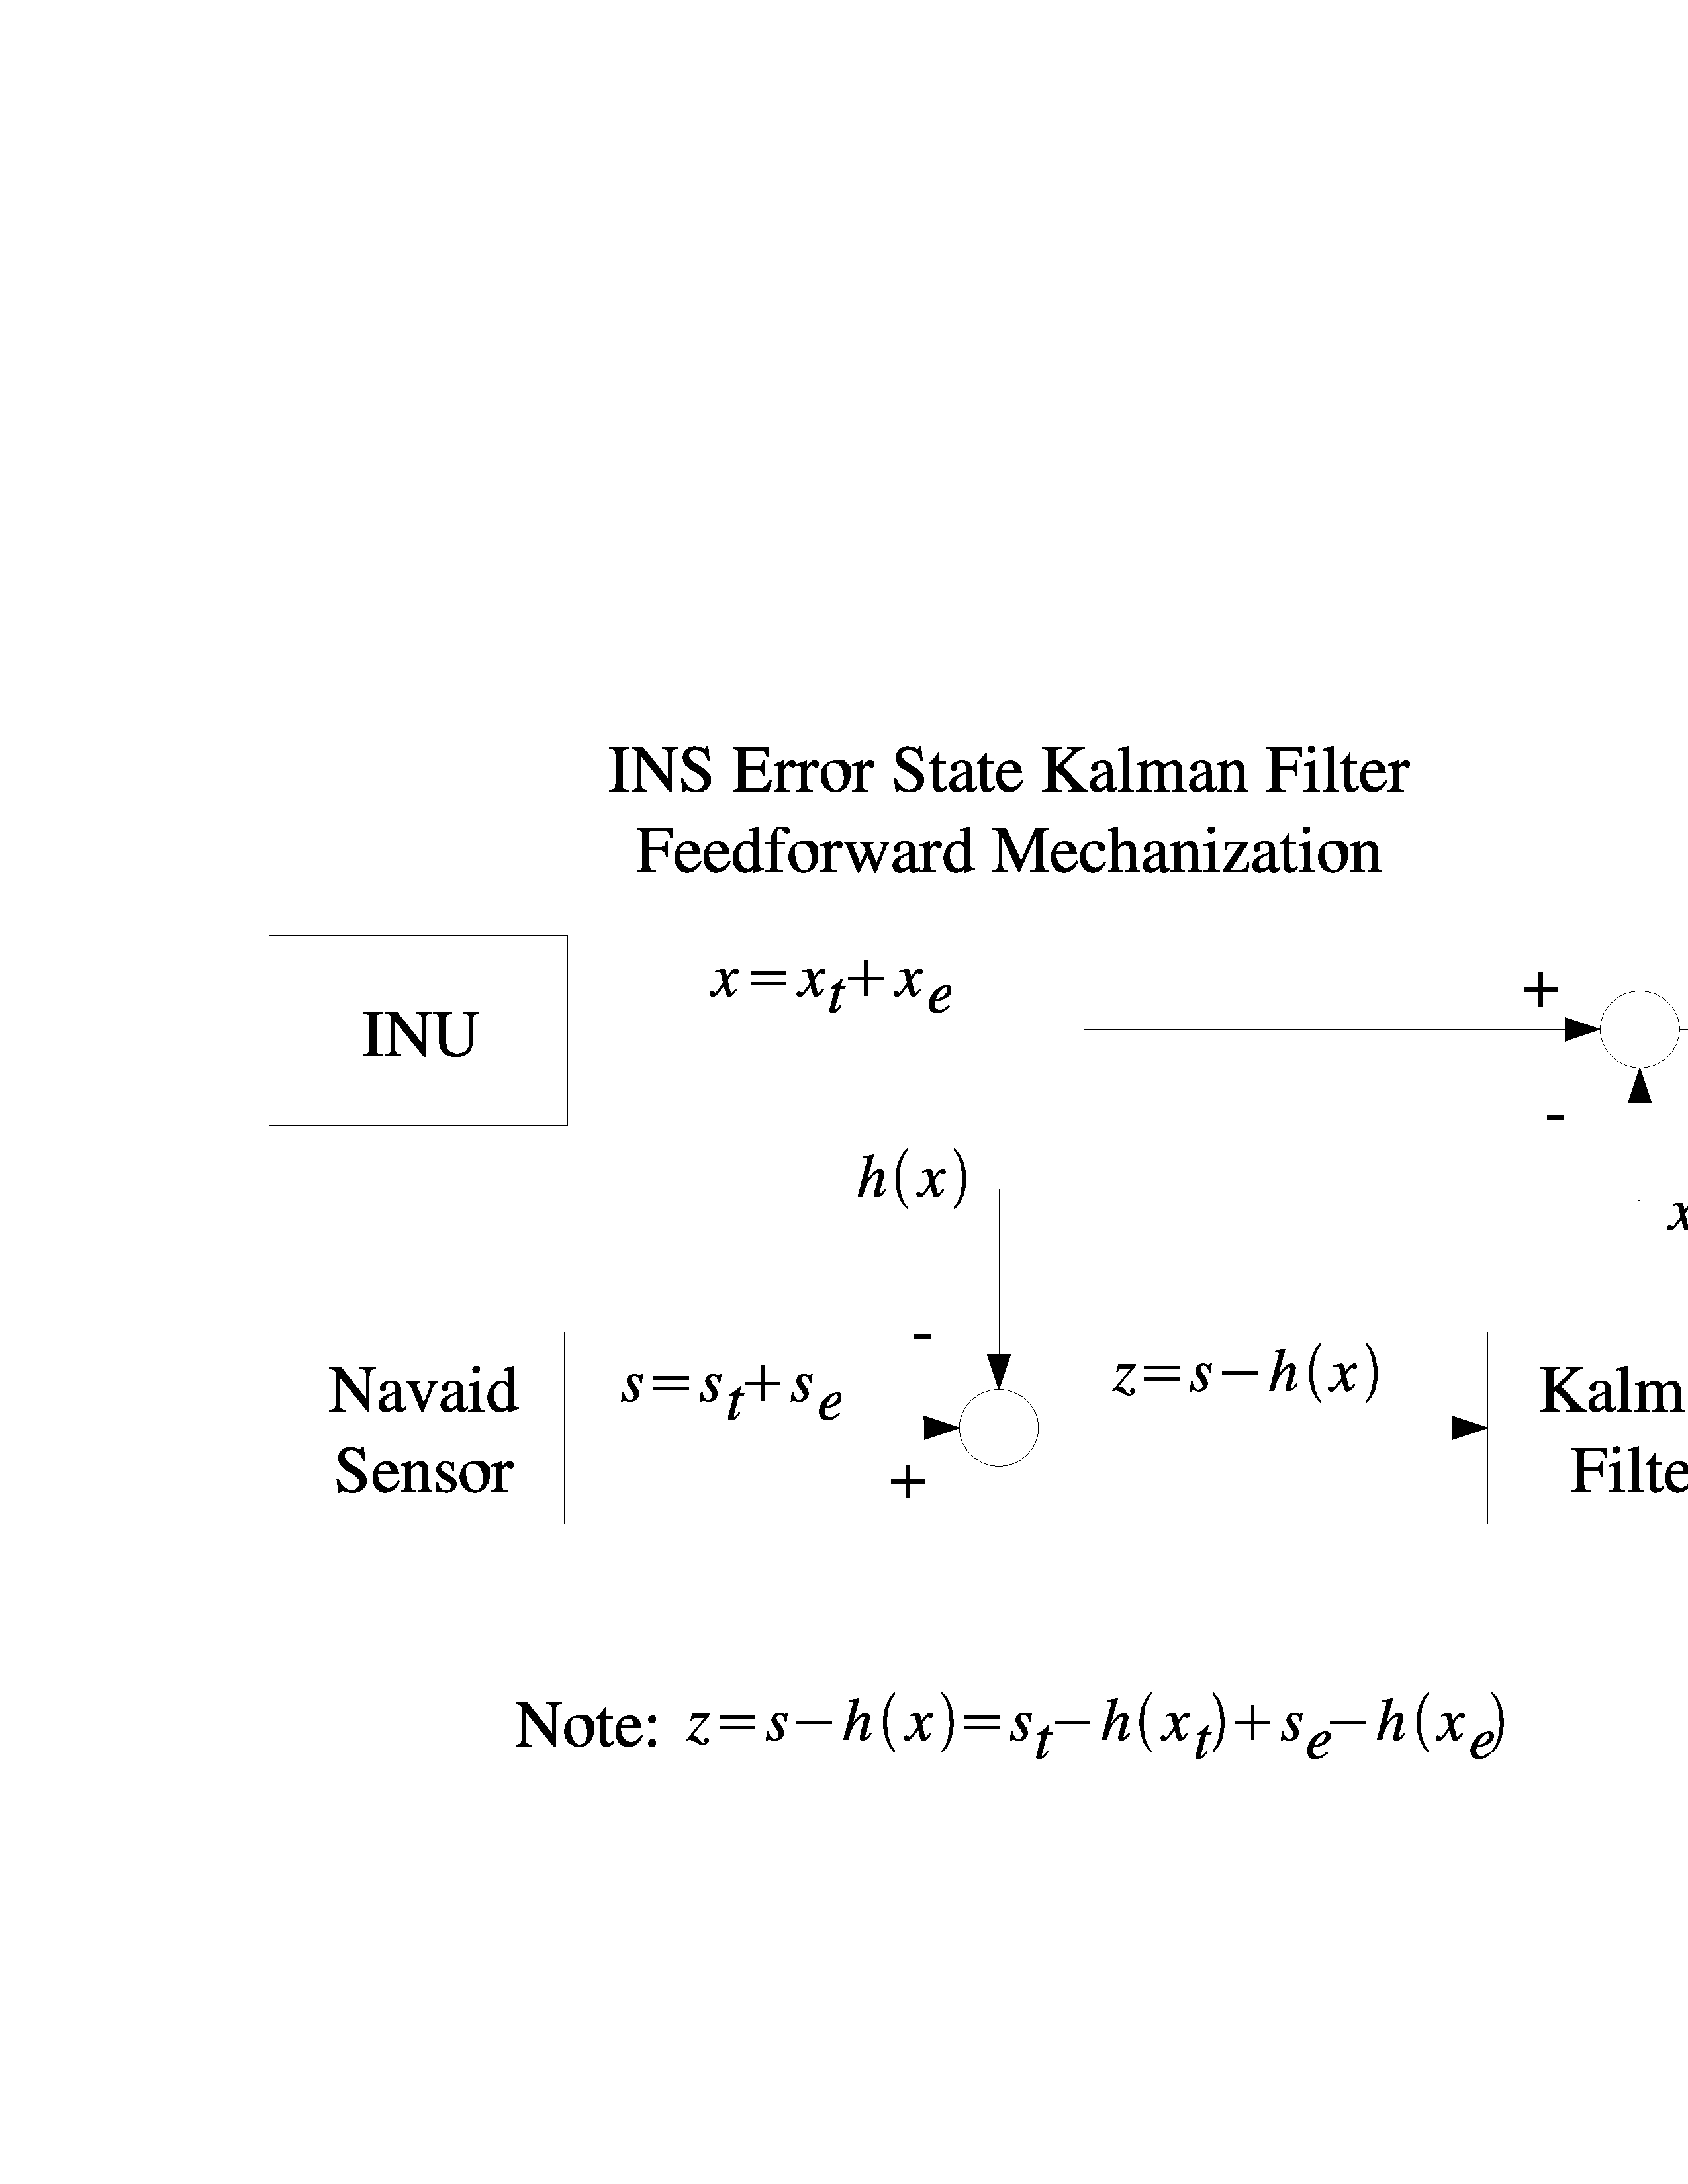
\includegraphics{day1_seg1_heuristic/feedforward.jpg}
\end{frame}

\begin{frame}
Navigation Aids (Navaids)
\begin{itemize}
  \item Measurement / Observation sources that aid in estimating INS error sources and dynamics
  \item Because we are interested in estimating INS errors, we use differencing to cancel out the whole state information
  \item INS outputs $x=x_t + x_e$, where $x_t$ is the true whole state information generated by INS, i.e., position, velocity, attitude, etc.
  \item Navaid sensor outputs $s=x_t+x_e$, where $x_t$ is once again the true quantities corrupted by sensor errors $x_e$.
\end{itemize} 
\end{frame}

\begin{frame}
Navigation Aids (Navaids)
\begin{itemize}
  \item Note that the navaid sensor usually only outputs part of the whole state vector, e.g., position and velocity, but not attitude (in the case of GPS)
  \item That's one reason why we have the $h$ function
  \item The INS signal is mapped by a linearized measurement function (or matrix) $h$ such that $h(x)=h(x_t) + h(x_e)$ and $h(x_t)=s_t$
\end{itemize} 
\end{frame}

\begin{frame}
Navigation Aids (Navaids)
\begin{itemize}
  \item Thus, we have
\begin{align*}
z&=s-h(x)\\
&=s_t + s_e - h(x_t) - h(x_e)\\
&=s_t - h(x_t) + s_e - h(x_e)\\
&=h(x_t) - h(x_t)+ s_e - h(x_e)\\
&=s_e - h(x_e)
\end{align*}
  \item Our measurement, therefore, is the difference between the navaid sensor errors and the INS errors
\end{itemize} 
\end{frame}

\begin{frame}
Navigation Aids (Navaids)
\begin{itemize}
  \item If $s_e$ is more than just white measurement noise, then we would need to model this vector in the filter according to known or assumed dynamics 
  \item Hence, sometimes adding a new navaid means adding new states to your filter

\end{itemize} 
\end{frame}

\begin{frame}
Navigation Aids (Navaids)
\begin{itemize}
  \item It is crucial to examine the innovations sequence for any non-white time correlations!
\[z_k-h\left[\stateest{k}{-}\right]=s_e(k)-h\left[(x_e(k)\right]-h\left[\stateest{k}{-}\right]\]
where we have added the index $k$ for clarity
 \item We should have $\expect{(z_k-h\left[\stateest{k}{-}\right])(z_j-h\left[\stateest{j}{-}\right])\trans}=0$ when $k\neq j$, which will in general be true provided $\expect{s_e(k)}=0$
 \item If this is not the case, then it is probably $s_e$ that is the culprit and you'd better start modeling!
\end{itemize} 
\end{frame}

\begin{frame}

\begin{itemize}
  \item The condition
\[\expect{(z_k-h\left[\stateest{k}{-}\right])(z_j-h\left[\stateest{j}{-}\right])\trans}=0
\]
says that the innovations sequence is uncorrelated in time.
  \item Recall that the innovations sequence is $\nu_k=z_k-h\left[\stateest{k}{-}\right]$
  \item Thus, we should have $\expect{\nu_k \nu_j\trans}=0$
  \item This means that the optimal estimator $\stateest{k}{+}$ always makes optimal use of the new information provided by $\nu_k$
\end{itemize} 
\end{frame}


% day4_seg2_navaids/gps.tex
\begin{frame}
GPS: The Global Positioning System
 \begin{itemize}
 \item 24+ satellites orbiting at 10,900 miles above surface
 \item Three Segments: Control, Space, User
 \item Time-tagged signals and known satellite position enable calculation of signal time of flight and hence range traversed from satellite to receiver
 \item Range to four satellites required to determine time plus three position coordinates
\end{itemize}
\end{frame}

\begin{frame}
GPS: The Global Positioning System
\begin{itemize}
  \item Satellites have precise atomic clocks
  \item User set receiver has less precise clock
  \item Time is of the essence:  comparing satellite-generated time-tag with user clock time of arrival determines transit time
  \item Note that user clock can be a source of systematic error
\end{itemize} 
\end{frame}

\begin{frame}
GPS: The Global Positioning System
\begin{itemize}
  \item Three types of navaid coupling:
  \begin{itemize}
	\item Loose coupling
    \item Tight coupling
    \item Deep coupling
  \end{itemize} 
\end{itemize} 
\end{frame}

\begin{frame}
Loosely-Coupled GPS
\begin{itemize}
  \item GPS receiver-generated position and velocity are differenced with INS position and velocity
  \item GPS position and velocity are generally pre-filtered (with a Kalman filter) before being used in inertial filter
  \item GPS position and velocity are also composite quantities from all satellites
  \item Least accurate approach to using GPS as a navaid
\end{itemize} 
\end{frame}

\begin{frame}
Loosely-Coupled GPS
\begin{itemize}
  \item The GPS receiver does not have the advantage of using inertial information to completely separate process noise from measurement noise
  \item Simplifies Kalman integration: Don't necessarily have to model GPS receiver clock errors (assume receiver has already done so)
\end{itemize} 
\end{frame}

\begin{frame}
Tightly-Coupled GPS
\begin{itemize}
  \item Pseudorange and delta pseudorange for each individual satellite are direct measurements presented to the filter
  \item Contains only measurement noise, not receiver filter's model of process noise 
  \item Gives INS filter more fine-grained control over GPS measurements
  \item Higher accuracy
\end{itemize} 
\end{frame}

\begin{frame}
Deeply-Coupled
\begin{itemize}
  \item Uses high-rate inertial data to aid in code and carrier phase tracking loops
  \item Most accurate solution when combined with tightly-coupled INS filter as well
\end{itemize} 
\end{frame}

\begin{frame}
GPS Errors
\begin{itemize}
  \item Ephemeris data: Satellite's reported position can be in error
  \item Satellite clock:  Negligible since SA (selective availability) has been turned off
  \item Ionosphere:  Pseudorange errors caused by free electrons in the ionosphere
\end{itemize} 
\end{frame}

\begin{frame}
GPS Errors (cont)
\begin{itemize}
  \item Troposphere: Pseudorange errors casued by temperature, pressure, humidity influences on the speed of light
  \item Multipath:  Errors casued by locking on to reflected signals
  \item Receiver Noise: Errors caused by receiver's thermal noise and software inaccuracies
\end{itemize} 
\end{frame}

\begin{frame}
\begin{center}
%\begin{tabular}{|c|p{2.5in}|p{2.5in} |} \hline
 \begin{tabular}{|p{3in}|p{1.5in}|p{1.5in}|} \hline
 % after \\ : \hline or \cline{col1-col2} \cline{col3-col4} ...
  \textbf{Error Source} & \textbf{C/A-Code Error Budget (meters)} & \textbf{P-Code Error Budget (meters)} \\ \hline
Multipath & 12.0 & 1.2 \\ \hline
Receiver Noise / Software & 11.1 & 1.1 \\ \hline
Ionosphereic Delays & 9.0 & 3.1 \\ \hline
Satellite Clock and  Ephemeris Errors & 3.9 & 3.9 \\ \hline
Tropspheric Delays & 2.0 & 2.0 \\ \hline
\end{tabular}
\end{center}
\end{frame}

\begin{frame}
Using Loosely-Coupled GPS Measurements
\begin{itemize}
  \item Position
	\begin{itemize}
		\item Form primary GPS position observation by subtracting Kalman-corrected INS reference position from raw GPS position
		\item Next, the innovation (or measurement residual) is formed by subtracting off the extrapolated state estimate of position error
		\item Extrapolated position error estimate needs to compensate for accumulated velocity error during Kalman cycle (or some fraction thereof) 
	\end{itemize}
\end{itemize} 
\end{frame}

\begin{frame}
An example (JOVIAL) from a transport aircraft navigation filter:
\end{frame}
\begin{verbatim}
  165  COMPUTE RESIDUALS 
  166      RESIDUALS(1) = Y'KAL'OBS(INU,1) * OBS'COUNT'SCALER - SVVAR(1)
  167 	- 5.0 * SVVAR(4);
  168      RESIDUALS(2) = Y'KAL'OBS(INU,2) * OBS'COUNT'SCALER - SVVAR(2)
  169 	- 5.0 * SVVAR(5);
  170      RESIDUALS(3) = Y'KAL'OBS(INU,7) * OBS'COUNT'SCALER - SVVAR(3)     
  171         - 5.0 * SVVAR(6);

\end{verbatim}

\begin{frame}
GPS Velocity Measurements
\begin{itemize}
  \item Based on carrier phase measurements in receiver
  \item Generally independent of position measurements
  \item Observation is once again difference between Kalman-compensated INS reference velocity and GPS-indicated velocity
\end{itemize} 
\end{frame}

\begin{frame}
GPS Measurment Noise Covariance
\begin{itemize}
  \item Based on EHE (estimated horizontal error) and EVE (estimated vertical error)
  \item These numbers highgly dependent on GDOPs
\end{itemize} 
\end{frame}

\begin{frame}
Geometric Dillution of Precision (GDOP)
\begin{itemize}
  \item Satellites are not geostationary
  \item H matrix is time-varying
  \item Observability varies with time
  \item $GDOP=\sqrt{\text{tr}\left(H\trans H\right)^{-1}}$
\end{itemize} 
\end{frame}


\begin{frame}
GDOP Chimney
\begin{itemize}
  \item Large DGOP is bad; normal values 3-5
  \item Singularity periods of time (about 1 hr) when GDOP values spike upward with a peak as much as 1000
  \item GDOP 50 $\approx$ 500 m position error
  \item Chimney's effects should be less acute if receiver has enough channels to track many satellites and to handle constellation changes
\end{itemize} 
\end{frame}


% day4_seg2_navaids/posfix.tex
\begin{frame}
Position Fix
 \begin{itemize}
 \item Overfly Fix
 \item Known location
 \item Delta formed between overfly location and indicated, Kalman-compensated INS position
 \item Usually a one-shot opportunity, i.e., not periodic like GPS
\end{itemize}
\end{frame}

% day4_seg2_navaids/radar.tex
\begin{frame}
Radar Fixes
 \begin{itemize}
 \item Instantaneous azimuth and elevation angles to a target of known latitude and longitude
 \item Or converted to local Cartesian coordinates (north, east, and altitude)
 \item Amount of cursor movement required to align curson with target yields position fix delta
 \item Otherwise, processed in filter like GPS or visual position fix
\end{itemize}
\end{frame}

% day4_seg2_navaids/dvs.tex
\begin{frame}
Doppler Velocity Sensor (DVS)
 \begin{itemize}
 \item DVS provides genuine velocity measurement with respect to ground
 \item DVS provides heading and drift velocities $V_H$ and $V_D$
 \item Nonlinear measurement relationship to INS-indicated velocities $V_x$ and $V_y$ and platform azimuth $\beta$:
\end{itemize}
\begin{align*}
V_H &= -V_x\sin\beta + V_y\cos\beta\\
V_D &=  V_x\cos\beta + V_y\sin\beta
\end{align*}
\end{frame}

\begin{frame}
DVS
\begin{itemize}
  \item Relationship between $(V_x,V_y)$ and $(V_H,V_D)$ is non-linear $h$
  \item To generate a linearized $H$ matrix we compute partial derivatives (Jacobians) to yield:
\[H=
\begin{bmatrix}
0&-\sin\beta&0&0&\cos\beta&0&0&0&-V_x\cos\beta - V_y\sin\beta\\
0&\cos\beta&0&0&\sin\beta&0&0&0&-V_x\sin\beta + V_y\cos\beta
\end{bmatrix}
\]
for a canonical 9-state filter.
\end{itemize} 
\end{frame}

% day4_seg2_navaids/tracking.tex
\begin{frame}
External Tracking Aids
 \begin{itemize}
 \item External platform tracks your vehicle and sends position / velocity info (JTIDS) 
 \item Bearing and distance measurments
	\begin{itemize}
		\item VOR, DME, TACAN
	\end{itemize}
\end{itemize}
\end{frame}

%% day4_seg2_navaids/att.tex
\begin{frame}
Attitude References
 \begin{itemize}
 \item 
 \item
 \item
\end{itemize}
\end{frame}

% day4_seg2_navaids/dted.tex
\begin{frame}
Digital Terrain Elevation Data (DTED)
 \begin{itemize}
 \item Published by National Geospatial Intelligence Agency (NGA)
	\begin{itemize}
		\item formerly NIMA, formerly DMA
	\end{itemize}
 \item 1 deg geocells of terrain height for each lat/long pair
 \item DTED Levels 0,1,2
\end{itemize}
\end{frame}

\begin{frame}
DTED
\begin{itemize}
  \item As navaid, a trail of radar altimeter measurements are stored
  \item Trail is correlated with DTED to determine offset
  \item SITAN, TERPROM
\end{itemize} 
\end{frame}

%% day4_seg2_navaids/exercises.tex
\begin{frame}
Exercises
 \begin{itemize}
 \item
 \item
 \item
\end{itemize}
\end{frame}


% day4_seg3_maint/maint_main.tex
\begin{frame}
\textbf{Day 4, Segment 3\\
Filter Maintenance\\
Topics}
 \begin{itemize}
 \item Filter Performance and Integrity Monitoring
 \item Replacing Navaids
 \item Adding New Navaids
 \item Augmenting the State Vector
\end{itemize}
\end{frame}
% day4_seg3_maint/perf_integ.tex
\begin{frame}
Filter Performance and Integrity Monitoring
 \begin{itemize}
 \item Covariance Monitoring
 \item Innovations Monitoring
 \item Corrective Action
\end{itemize}
\end{frame}
\begin{frame}
Covariance Monitoring
\begin{itemize}
  \item Ensuring Symmetry
  \item Managing Observability
  \item Ensuring Positive Definiteness
\end{itemize} 
\end{frame}
\begin{frame}
Covariance Monitoring:  Ensuring Symmetry
\begin{itemize}
  \item $P$ is supposed to be positive definite and symmetric
  \item Symmetry means that $P\trans = P$, i.e., for each element $p_{ij}$ of $P$ we must have $p_{ij}=p_{ji}$
  \item Roundoff error can cause loss of symmetry
  \item The best way to ensure symmetry is to work only with items on or (say) above the diagonal and simply define elements below he diagonal by fiat.
\end{itemize} 
\end{frame}
\begin{frame}
Covariance Monitoring:  Ensuring Symmetry
\begin{itemize}
  \item Both $P(+)$ and $P(-)$ need to be symmetrized
\begin{itemize}
  \item After extrapolation: symmetrize
  \item After update: symmetrize
\end{itemize}
\end{itemize} 
\end{frame}
\begin{frame}
Covariance Monitoring:  Managing Observability
\begin{itemize}
  \item Observability means there is a linear path from the measurements to states
  \item Structural observability determined by $\Phi$ and $H$:
\end{itemize}
 If $H$ is $1\times n$, where $n$ is the size of the state vector, then the state $x_0$ is said to be \textbf{observable }from $n$ scalar measurements $\set{z_0,\ldots,z_{n-1}}$ if the block matrix
\[
\begin{bmatrix}
H\trans&\Phi\trans H\trans & \cdots & (\Phi\trans)^{n-1}H\trans
\end{bmatrix}
\]
is of rank $n$
\end{frame}
\begin{frame}
Covariance Monitoring:  Managing Observability
\begin{itemize}
  \item If unobservable states are also unstable, estimation errors will be unstable and $P$ will show symptoms 
\begin{itemize}
  \item $\text{diag}(P)\rightarrow \infty$
  \item I.e., one or more diagonal elements of $P$ will grow without bound
\end{itemize}
  \item Not the same as divergence: "feature" of the design
\end{itemize}
\end{frame}
\begin{frame}
Covariance Monitoring:  Managing Observability
\begin{itemize}
  \item Note also that the state estimation error variances (i.e., the diagonals of $P$) will naturally grow in the absence of measurements
  \item Going for a long time without incorporating a measurement is equivalent to lack of observability in the associated states
  \item Use covariance analysis simulation to detect non-observability
  \item The only real solution is to add new measurements
\end{itemize}
\end{frame}
\begin{frame}
Covariance Monitoring:  Ensuring Positive Definiteness
\begin{itemize}
  \item $P$ is supposed to be positive definite
  \item This means that $x'Px>0$ whenever $x\neq0$
  \item States modeled as random constants or other deterministic states can cause loss of positivity
  \item Add covariance bumping:  Add small amounts of process noise to diagonal elements of $Q$ for these states
\end{itemize}
\end{frame}

% day4_seg3_maint/replace_navaids.tex
\begin{frame}
Replacing Navaids
 \begin{itemize}
 \item Replacing a given sensor with another of the same type usually requires no changes to the state model
	\begin{itemize}
		\item unless replacement sensor has significant errory dynamics that need to be modeled (see adding new sensors and state augmentation)
	\end{itemize}
 \item Measurement noise covariance generally has to change however
\end{itemize}
\end{frame}

% day4_seg3_maint/new_navaids.tex
\begin{frame}
Adding New Navaids
 \begin{itemize}
 \item What kinds of navaids are desirable?
 \item What are the steps involved in adding a new navaid?
\end{itemize}
\end{frame}
\begin{frame}
Adding New Navaids\\
Desirable Characteristics:
\begin{itemize}
  \item Navaids which render observable otherwise unobservable states
  \item Those having a simple relationship (preferably linear) to the state vector
  \item Having only white noise error dynamics
\end{itemize} 
\end{frame}

% day4_seg3_maint/aug_state_vec.tex
\begin{frame}
Augmenting the State Vector
 \begin{itemize}
 \item State Vector Augmentation: Expanding the size of the state vector
\begin{itemize}
	\item i.e., adding new states
\end{itemize}
 \item Why?
\begin{itemize}
	\item new navaids with their own error dynamics (e.g., GPS)
	\item correlated (non-white) process noise
	\item correlated (non-white) measurement noise
\end{itemize}
\end{itemize}
\end{frame}
\begin{frame}
Augmenting the State Vector
\begin{itemize}
  \item Why? (continued)
\begin{itemize}
  \item Correlation $\Rightarrow$ dynamics
\begin{itemize}
	\item No dynamics in white noise
\end{itemize}
  \item If dynamics are present they must be modeled
  \item Otherwise, dynamic effects will be allocated to other states
\end{itemize} 
\end{itemize} 
\end{frame}
\begin{frame}
Augmenting the State Vector
\begin{itemize}
 \item How?
\begin{itemize}
	\item model non-white noise as result of feeding white noise through a linear system
	\item new states are outputs of new integrators
\end{itemize}
  \item State transition matrix $\Phi$ and error covariance matrix $P$ grow as $j^2$, where $j$ is number of new states
  \item Geometry matrix $H$ grows as $m\cdot j$, where $m$ is number of measurements and $j$ is number of new states
\end{itemize} 
\end{frame}
\begin{frame}
Augmenting the State Vector\\
Example: Ship Inertial Navigation Systems (SINS)
\begin{itemize}
  \item Long mission times
\begin{itemize}
	\item Especially submarines
\end{itemize}
  \item Position fixes insufficient to calibrate gyro bias drift w/o further modeling
\end{itemize} 
\end{frame}
\begin{frame}
Augmenting the State Vector\\
Example: Ship Inertial Navigation Systems (SINS)
\begin{itemize}
  \item Gyro bias drift due to slowly changing bias
  \item Can be modeled as random walk
  \item Random walk modeled as integrated white noise
  \item Kalman filter needed to estimate drift 
\end{itemize} 
\end{frame}
\begin{frame}
Augmenting the State Vector\\
Example: Ship Inertial Navigation Systems (SINS)
\begin{itemize}
  \item Assume platform tilts are kept close to zero through velocity measurements damping the Schuler oscillations
  \item North-West-Up (NWU) coordinate frame (or West-South-Up)
\end{itemize} 
\end{frame}
\begin{frame}
Augmenting the State Vector\\
Example: Ship Inertial Navigation Systems (SINS)
\begin{itemize}
  \item Two angular position errors in radians:  $\psi_N$ and $\psi_W$
\begin{itemize}
	\item Note $\psi_N$ is a small angular rotation about the north axis and  thus induces a west position error.
    \item Similarly, $\psi_W$ is a small rotation about the west axis and thus induces a south position error.
\end{itemize}
  \item $\theta_U =\psi_Z - \psi_N \tan(\lambda)$, where $\psi_Z$ is platform azimuth error and $\lambda$ is the latitude.
\end{itemize} 
\end{frame}
\begin{frame}
Augmenting the State Vector\\
Example: Ship Inertial Navigation Systems (SINS)
\begin{itemize}
  \item Error Dynamics:
\begin{align*}
\dot{\psi}_N - \Omega_U\psi_W &= \delta g_N\\
\dot{\psi}_W + \Omega_U \psi_N - \Omega_N\theta_U &= \delta g_W\\
\dot{\theta}_U + \Omega_N \psi_W &= \delta g_U
\end{align*}
where $\delta g_N,\delta g_W,\delta g_U$ are non-white gyro bias drift errors and $\Omega_N=\Omega\cos(\lambda)$ and $\Omega_U=\Omega\sin(\lambda)$ are components of earth rate
\end{itemize} 
\end{frame}
\begin{frame}
Augmenting the State Vector\\
Example: Ship Inertial Navigation Systems (SINS)
\begin{itemize}
  \item Since $\delta g_N,\delta g_W,\delta g_U$ are non-white, the question arises as to what kind of model is appropriate
  \item Empirical data indicates that gyro biases exhibit random walk behavior over time
  \item Since random walk is the integral of white noise, white noise can be viewed (in some sense) as the derivative of random walk
\end{itemize} 
\end{frame}
\begin{frame}
Augmenting the State Vector\\
Example: Ship Inertial Navigation Systems (SINS)
\begin{itemize}
  \item Hence, the following dynamics of random walk apply:
\begin{align*}
\dot{\delta} g_N &= w_N\\
\dot{\delta} g_W &= w_W\\
\dot{\delta} g_U &= w_U
\end{align*}
where $w_N,w_W,w_U$ are white noise processes.
\end{itemize} 
\end{frame}
\begin{frame}
Augmenting the State Vector\\
Example: Ship Inertial Navigation Systems (SINS)
\begin{itemize}
  \item We use the random walk equations to augment the state dynamics equations
  \item Thus we now have a six-state model:
\end{itemize} 
\[
\begin{bmatrix}
\dot{\psi}_N\\
\dot{\psi}_W\\
\dot{\theta}_U\\
\dot{\delta} g_N\\
\dot{\delta} g_W\\
\dot{\delta} g_U
\end{bmatrix}
=
\begin{bmatrix}
0&\Omega_U&0&1&0&0\\
-\Omega_U&0&\Omega_N&0&1&0\\
0&-\Omega_N&0&0&0&1\\
0&0&0&0&0&0\\
0&0&0&0&0&0\\
0&0&0&0&0&0
\end{bmatrix}
\begin{bmatrix}
\psi_N\\
\psi_W\\
\theta_U\\
\delta g_N\\
\delta g_W\\
\delta g_U
\end{bmatrix}
+\begin{bmatrix}
0&0&0&0&0&0\\
0&0&0&0&0&0\\
0&0&0&0&0&0\\
0&0&0&1&0&0\\
0&0&0&0&1&0\\
0&0&0&0&0&1
\end{bmatrix}
\begin{bmatrix}
0\\
0\\
0\\
w_N\\
w_W\\
w_U
\end{bmatrix}
\]
\end{frame}
\begin{frame}
Augmenting the State Vector:  Summary
\begin{itemize}
  \item Straightforward: When new, relevant dynamic relations found, simply add the states to the state vector and add the new dynamics to the $F$ and/or $\Phi$ matrix
  \item Use basic models such as low-order systems driven by white noise to model new states
\end{itemize}
\end{frame}
\begin{frame}
Augmenting the State Vector:  Summary
\begin{itemize}
  \item Some Popular Models
\begin{itemize}
	\item random walk
	\item random constant
	\item random ramp
	\item Gauss-Markov (i.e., exponentially correlated)
	\item combinations of the above!
\end{itemize}
\end{itemize} 
\end{frame}


% day4_seg3_maint/exercises.tex
\begin{frame}
Exercises
 \begin{enumerate}
 \item Write a simple 1-state model for a gyro bias modeled as a random constant
 \item Now augment this model to a 2-state model by adding a random walk
\end{enumerate}
\end{frame}


% day4_seg4_redund/redund_main.tex
\begin{frame}
\textbf{Day 4, Segment 4\\
Filter Redundancy and Fault Tolerance\\
Topics}
 \begin{itemize}
 \item Typical Weighting Scheme
 \item Detecting Faults
 \item Graceful Degradation
\end{itemize}
\end{frame}
% day4_seg4_redund/ct_weighting.tex
\begin{frame}
Typical Weighting Scheme
 \begin{itemize}
 \item Two separate INS error dynamics filters
 \item Use error covariance outputs from each filter to weight state estimates
\end{itemize}
\end{frame}

\begin{frame}
Typical Weighting Scheme
 \begin{itemize}
 \item Weighting scheme:
\[w_i(x)=\dfrac{\sigma_j(x)}{\sigma_1(x)+\sigma_2(x)}\]
where $i\neq j\in\set{1,2}$ and $x$ is the parameter in question
\end{itemize}
\end{frame}

\begin{frame}
Alternatives to Weighting: Decentralized Filtering
\begin{itemize}
  \item Decentralized filtering without feedback
  \item Decentralized filtering with feedback
\end{itemize} 
\end{frame}

\begin{frame}
Decentralized Filtering without Feedback
\begin{itemize}
  \item Assume two local filters
  \item Then for the global error covariance we have:
\[P^{-1}=P_1^{-1}+M_1^{-1}+P_2^{-1}+M_2^{-1}+M^{-1}\]
where $P_1,P_2$ are updated local error covariances for each filter, $M_1,M_2$ are extrapolated local error covariances prior to update, and $M$ is the global filter's prior error covariance.
\end{itemize} 
\end{frame}

\begin{frame}
Decentralized Filtering without Feedback
\begin{itemize}
  \item The global filter's estimate is
\[\hat{x}=P\left[P_1^{-1}\hat{x}_1-M_1m_1^{-1}+P_2^{-1}\hat{x}_2-M_2m_2^{-1}+M^{-1}m\right]\]
where $m_1,m_2,m$ are the local a priori estimates for local filters 1 and 2 and the global filter, respectively.
\end{itemize} 
\end{frame}

%% day4_seg4_redund/fault_detection.tex
\begin{frame}
Detecting Faults
 \begin{itemize}
 \item
 \item
 \item
\end{itemize}
\end{frame}

%% day4_seg4_redund/graceful_deg.tex
\begin{frame}
Graceful Degradation
 \begin{itemize}
 \item
 \item
 \item
\end{itemize}
\end{frame}

% day4_seg4_redund/exercises.tex
\begin{frame}
Exercises
 \begin{enumerate}
 \item Let the x position error variance for filter 1 be 4 meters, that of filter 2 16 meters.  Calculate the weighted average latitude given lat1=33.3 deg, lat2=33.21.   
 \item How would the decentralized filter's estimate differ from the weighted average?
\end{enumerate}
\end{frame}


% ----------------------------------------------------------------
\end{document}
